% =====================================================================
%  ARCHIVO MAESTRO DEL INFORME -- Proyecto Final de Química Orgánica
%  Plantilla base: Journal of Computational Science and Applications (JCSA)
%  (plantilla oficial suministrada por el docente)
%
%  Estructura modular:
%     main.tex                 -> preámbulo, título, resumen, unión de partes
%     Sara/sara.tex            -> Introducción, Marco Teórico, Tabla de datos
%     Valentina/valentina.tex  -> Metodología, Análisis Gráfico, Conclusiones
%     references.bib           -> bibliografía compartida (BibLaTeX + Biber)
%     imagenes/                -> figuras exportadas desde Google Colab
%
%  Compilación: pdflatex -> biber -> pdflatex -> pdflatex
% =====================================================================
\documentclass[twoside,twocolumn,10pt]{article}
\usepackage[utf8]{inputenc}
\usepackage[T1]{fontenc}
\usepackage{fancyhdr}
\usepackage{geometry}
\usepackage{multicol}
\usepackage{abstract}
\usepackage{graphicx}
\graphicspath{{imagenes/}}
\usepackage{threeparttable}
\usepackage{titlesec}
\usepackage{ragged2e}  % Provides the justifying command
\usepackage{amssymb}   % For additional symbols
\usepackage{parskip}   % Automatically handles paragraph spacing
\usepackage{amsmath}   % For advanced math environments
\usepackage{newtxtext} % Times New Roman font
\usepackage{booktabs}  % For improved table appearance
\usepackage{array}     % For customizing table columns
\usepackage{siunitx}   % Unidades químicas (g/mol, °C, g/cm^3)
\sisetup{output-decimal-marker={,}}
\usepackage[spanish,es-tabla]{babel} % es-tabla: "Tabla" en vez de "Cuadro"
\usepackage[
	backend=biber,
	style=chem-acs, 	% Aplica el estilo compacto de revistas científicas
	articletitle=false,
	maxnames=4,
	minnames=1
]{biblatex}
\usepackage[version=4]{mhchem} % Notación química: \ce{CH3NH2}
\addbibresource{references.bib}
\setcounter{page}{1}

% Define custom column types for better alignment and spacing
\newcolumntype{L}[1]{>{\raggedright\arraybackslash}p{#1}} % Left aligned column
\newcolumntype{C}[1]{>{\centering\arraybackslash}p{#1}}   % Center aligned column
\newcolumntype{R}[1]{>{\raggedleft\arraybackslash}p{#1}}  % Right aligned column

\usepackage[font=footnotesize, labelfont=bf, justification=raggedright, format=plain]{caption}

\captionsetup[table]{
    labelsep=period,
    justification=raggedright
}

\captionsetup[figure]{
    labelsep=period,
    justification=raggedright
}

% Set page margins
\geometry{
    letterpaper,
    left=0.8in,
    right=0.8in,
    top=1in,
    bottom=1in
}

% Increase space between columns
\setlength{\columnsep}{20pt}

% Define the centred abstract heading
\renewcommand{\abstractname}{\hspace{1.3em}\textbf{Resumen}}

\titleformat{\section}{\large\bfseries\uppercase}{\thesection.}{1em}{}
\titleformat{\subsection}{\normalfont\bfseries\flushleft}{\thesubsection.}{1em}{}
\titleformat{\subsubsection}{\normalfont\bfseries\itshape\flushleft}{\thesubsubsection}{1em}{}

% Set font sizes for abstract
\renewcommand{\abstractnamefont}{\normalfont\fontsize{14}{20}\bfseries}
\renewcommand{\absnamepos}{flushleft}
\renewcommand{\abstracttextfont}{\normalfont\fontsize{11}{13}\selectfont}

\hyphenpenalty=10000
\exhyphenpenalty=10000
\sloppy

% Set up header and footer styles
\pagestyle{fancy}
\fancyhf{}
\fancyhead[CO]{\small Propiedades fisicoquímicas de aminas y amidas}
\fancyhead[CE]{\small Proyecto de Química Orgánica (2026)}
\fancyfoot[C]{\thepage}

% First page custom header/footer
\fancypagestyle{firstpage}{
  \fancyhf{}
  \fancyhead[LO]{\small Ingeniería Ambiental, FAMARENA-UD}
  \fancyhead[RO]{\small QUIMORG 2026-III}
  \fancyfoot[L]{\footnotesize Impreso: \today \\\textsuperscript{*}Autor de correspondencia: Nombre Completo \textless correo@udistrital.edu.co\textgreater}
  \fancyfoot[R]{\footnotesize \copyright\ 2026 por los Autores. Publicado para proyecto final,\\\textsuperscript{*} bajo protección de difusión }
  \renewcommand{\headrulewidth}{0.4pt}
  \renewcommand{\footrulewidth}{0.4pt}
}

% ---------------------------------------------------------------------
%  TÍTULO Y AUTORES  (editar nombres completos)
% ---------------------------------------------------------------------
\title{\fontsize{16}{20}\selectfont\textbf{Relación estructura--propiedad en aminas y amidas: análisis estadístico de propiedades fisicoquímicas obtenidas de CAS-SciFinder}}
\author{
    \fontsize{12}{14}\selectfont
    Sara [Apellido]\textsuperscript{1*}, Valentina [Apellido]\textsuperscript{1}, [Tercer integrante]\textsuperscript{1}\\[1ex]
    \fontsize{12}{14}\selectfont
    \textsuperscript{1}Ingeniería Ambiental, Facultad del Medio Ambiente y Recursos Naturales,\\
    Universidad Distrital Francisco José de Caldas, Bogotá, Colombia
}
\date{}

\begin{document}

\twocolumn[
\begin{@twocolumnfalse}
\vspace{-0.5cm}
\raggedright

{\fontsize{11}{13}\selectfont{Artículo de Investigación}}
\vspace{-0.8cm}

\maketitle

\thispagestyle{firstpage}
\begin{abstract}
\fontsize{11}{13}\selectfont
\vspace{1em}
\justifying
% TODO (grupo): redactar el resumen al final, en un solo párrafo de 150--250 palabras:
% objetivo, fuente de datos (CAS-SciFinder), herramientas (Python, Power BI),
% resultados principales (correlaciones) y conclusión principal.
\textit{[Resumen pendiente: un párrafo de 150--250 palabras con objetivo, metodología, resultados principales y conclusión.]}

\vspace{-0.1cm}
\noindent\textbf{Palabras clave:}
 aminas, amidas, puentes de hidrógeno, punto de ebullición, correlación de Spearman.

\end{abstract}

\vspace{1cm}
\end{@twocolumnfalse}
]

% ---------------------------------------------------------------------
%  PARTE DE SARA: Introducción, Marco Teórico y Tabla de datos
% ---------------------------------------------------------------------
% =====================================================================
%  PARTE DE SARA  --  se incluye desde main.tex con % =====================================================================
%  PARTE DE SARA  --  se incluye desde main.tex con % =====================================================================
%  PARTE DE SARA  --  se incluye desde main.tex con \input{Sara/sara}
%  Contenido: Introducción, Marco Teórico y Tabla de datos
%
%  Reglas para editar sin romper la compilación:
%   * NO escribir \documentclass, \begin{document} ni \end{document} aquí.
%   * Citas: agregar la referencia en ../references.bib y citar con \cite{clave}.
%   * Fórmulas químicas: \ce{CH3NH2}, \ce{(CH3)2NH}, \ce{CH3CONH2}.
%   * Unidades: \si{\gram\per\mole}, \si{\degreeCelsius}, \si{\gram\per\centi\metre\cubed}.
% =====================================================================

\section{Introducción}
\fontsize{12}{14}\selectfont
% TODO (Sara): pegar aquí la redacción de la introducción.
% Sugerencia de hilo argumentativo:
%  1. Importancia de los compuestos nitrogenados (aminas y amidas) en química
%     orgánica, biología y en el ambiente.
%  2. Problema: cómo la estructura (grado de sustitución del N, grupo carbonilo,
%     capacidad de formar puentes de hidrógeno) determina las propiedades físicas.
%  3. Objetivo del trabajo: relacionar estadísticamente propiedades obtenidas en
%     CAS-SciFinder (PM, pf, P.eb, densidad, pKa, momento dipolar, solubilidad).
\textit{[Redacción de la introducción pendiente.]}

Los datos de partida se obtuvieron de CAS-SciFinder \cite{1_Su2022}.
% (Reemplazar esta cita de ejemplo por la referencia real de CAS-SciFinder.)

\section{Marco Teórico}
\fontsize{12}{14}\selectfont
% TODO (Sara): pegar aquí la redacción del marco teórico.
% Temas sugeridos:
%  * Aminas primarias, secundarias y terciarias: \ce{CH3NH2}, \ce{(CH3)2NH}, \ce{(CH3)3N}.
%  * Amidas: acetamida, N-metilacetamida, N,N-dimetilacetamida, urea.
%  * Fuerzas intermoleculares: puentes de hidrógeno N--H$\cdots$N y N--H$\cdots$O,
%    dipolo--dipolo y dispersión de London.
%  * Basicidad (pKa del ácido conjugado) y efecto de la resonancia en amidas.

\subsection{Fuerzas intermoleculares}
\textit{[Redacción pendiente.]}

\subsection{Basicidad y resonancia}
\textit{[Redacción pendiente.]}

\subsection{Tabla de datos de propiedades químicas}
\label{sec:tabla}
% TODO (Sara): completar la tabla con los valores definitivos del Excel
% (Datos/datos_power_bi.xlsx). Una fila por compuesto; usar "--" si falta el dato.
La Tabla~\ref{tab:propiedades} resume las propiedades fisicoquímicas de los
compuestos estudiados, consolidadas desde CAS-SciFinder.

\begin{table}[htbp]
	\centering
	\captionsetup{width=\columnwidth, justification=justified}
	\caption{Propiedades fisicoquímicas de los compuestos estudiados.}
	\label{tab:propiedades}
	\resizebox{\columnwidth}{!}{%
		\begin{tabular}{lccccc}
			\toprule
			\textbf{Compuesto} & \textbf{PM} & \textbf{pf} & \textbf{P.eb} & \textbf{$\rho$} & \textbf{pKa} \\
			 & (\si{\gram\per\mole}) & (\si{\degreeCelsius}) & (\si{\degreeCelsius}) & (\si{\gram\per\centi\metre\cubed}) & \\
			\midrule
			Metilamina            & -- & -- & -- & -- & -- \\
			Dimetilamina          & -- & -- & -- & -- & -- \\
			Trimetilamina         & -- & -- & -- & -- & -- \\
			N-metiletanamina      & -- & -- & -- & -- & -- \\
			Bencidina             & -- & -- & -- & -- & -- \\
			Acetamida             & -- & -- & -- & -- & -- \\
			N-metilacetamida      & -- & -- & -- & -- & -- \\
			N,N-dimetilacetamida  & -- & -- & -- & -- & -- \\
			Urea                  & -- & -- & -- & -- & -- \\
			\bottomrule
		\end{tabular}%
	}
\end{table}

%  Contenido: Introducción, Marco Teórico y Tabla de datos
%
%  Reglas para editar sin romper la compilación:
%   * NO escribir \documentclass, \begin{document} ni \end{document} aquí.
%   * Citas: agregar la referencia en ../references.bib y citar con \cite{clave}.
%   * Fórmulas químicas: \ce{CH3NH2}, \ce{(CH3)2NH}, \ce{CH3CONH2}.
%   * Unidades: \si{\gram\per\mole}, \si{\degreeCelsius}, \si{\gram\per\centi\metre\cubed}.
% =====================================================================

\section{Introducción}
\fontsize{12}{14}\selectfont
% TODO (Sara): pegar aquí la redacción de la introducción.
% Sugerencia de hilo argumentativo:
%  1. Importancia de los compuestos nitrogenados (aminas y amidas) en química
%     orgánica, biología y en el ambiente.
%  2. Problema: cómo la estructura (grado de sustitución del N, grupo carbonilo,
%     capacidad de formar puentes de hidrógeno) determina las propiedades físicas.
%  3. Objetivo del trabajo: relacionar estadísticamente propiedades obtenidas en
%     CAS-SciFinder (PM, pf, P.eb, densidad, pKa, momento dipolar, solubilidad).
\textit{[Redacción de la introducción pendiente.]}

Los datos de partida se obtuvieron de CAS-SciFinder \cite{1_Su2022}.
% (Reemplazar esta cita de ejemplo por la referencia real de CAS-SciFinder.)

\section{Marco Teórico}
\fontsize{12}{14}\selectfont
% TODO (Sara): pegar aquí la redacción del marco teórico.
% Temas sugeridos:
%  * Aminas primarias, secundarias y terciarias: \ce{CH3NH2}, \ce{(CH3)2NH}, \ce{(CH3)3N}.
%  * Amidas: acetamida, N-metilacetamida, N,N-dimetilacetamida, urea.
%  * Fuerzas intermoleculares: puentes de hidrógeno N--H$\cdots$N y N--H$\cdots$O,
%    dipolo--dipolo y dispersión de London.
%  * Basicidad (pKa del ácido conjugado) y efecto de la resonancia en amidas.

\subsection{Fuerzas intermoleculares}
\textit{[Redacción pendiente.]}

\subsection{Basicidad y resonancia}
\textit{[Redacción pendiente.]}

\subsection{Tabla de datos de propiedades químicas}
\label{sec:tabla}
% TODO (Sara): completar la tabla con los valores definitivos del Excel
% (Datos/datos_power_bi.xlsx). Una fila por compuesto; usar "--" si falta el dato.
La Tabla~\ref{tab:propiedades} resume las propiedades fisicoquímicas de los
compuestos estudiados, consolidadas desde CAS-SciFinder.

\begin{table}[htbp]
	\centering
	\captionsetup{width=\columnwidth, justification=justified}
	\caption{Propiedades fisicoquímicas de los compuestos estudiados.}
	\label{tab:propiedades}
	\resizebox{\columnwidth}{!}{%
		\begin{tabular}{lccccc}
			\toprule
			\textbf{Compuesto} & \textbf{PM} & \textbf{pf} & \textbf{P.eb} & \textbf{$\rho$} & \textbf{pKa} \\
			 & (\si{\gram\per\mole}) & (\si{\degreeCelsius}) & (\si{\degreeCelsius}) & (\si{\gram\per\centi\metre\cubed}) & \\
			\midrule
			Metilamina            & -- & -- & -- & -- & -- \\
			Dimetilamina          & -- & -- & -- & -- & -- \\
			Trimetilamina         & -- & -- & -- & -- & -- \\
			N-metiletanamina      & -- & -- & -- & -- & -- \\
			Bencidina             & -- & -- & -- & -- & -- \\
			Acetamida             & -- & -- & -- & -- & -- \\
			N-metilacetamida      & -- & -- & -- & -- & -- \\
			N,N-dimetilacetamida  & -- & -- & -- & -- & -- \\
			Urea                  & -- & -- & -- & -- & -- \\
			\bottomrule
		\end{tabular}%
	}
\end{table}

%  Contenido: Introducción, Marco Teórico y Tabla de datos
%
%  Reglas para editar sin romper la compilación:
%   * NO escribir \documentclass, \begin{document} ni \end{document} aquí.
%   * Citas: agregar la referencia en ../references.bib y citar con \cite{clave}.
%   * Fórmulas químicas: \ce{CH3NH2}, \ce{(CH3)2NH}, \ce{CH3CONH2}.
%   * Unidades: \si{\gram\per\mole}, \si{\degreeCelsius}, \si{\gram\per\centi\metre\cubed}.
% =====================================================================

\section{Introducción}
\fontsize{12}{14}\selectfont
% TODO (Sara): pegar aquí la redacción de la introducción.
% Sugerencia de hilo argumentativo:
%  1. Importancia de los compuestos nitrogenados (aminas y amidas) en química
%     orgánica, biología y en el ambiente.
%  2. Problema: cómo la estructura (grado de sustitución del N, grupo carbonilo,
%     capacidad de formar puentes de hidrógeno) determina las propiedades físicas.
%  3. Objetivo del trabajo: relacionar estadísticamente propiedades obtenidas en
%     CAS-SciFinder (PM, pf, P.eb, densidad, pKa, momento dipolar, solubilidad).
\textit{[Redacción de la introducción pendiente.]}

Los datos de partida se obtuvieron de CAS-SciFinder \cite{1_Su2022}.
% (Reemplazar esta cita de ejemplo por la referencia real de CAS-SciFinder.)

\section{Marco Teórico}
\fontsize{12}{14}\selectfont
% TODO (Sara): pegar aquí la redacción del marco teórico.
% Temas sugeridos:
%  * Aminas primarias, secundarias y terciarias: \ce{CH3NH2}, \ce{(CH3)2NH}, \ce{(CH3)3N}.
%  * Amidas: acetamida, N-metilacetamida, N,N-dimetilacetamida, urea.
%  * Fuerzas intermoleculares: puentes de hidrógeno N--H$\cdots$N y N--H$\cdots$O,
%    dipolo--dipolo y dispersión de London.
%  * Basicidad (pKa del ácido conjugado) y efecto de la resonancia en amidas.

\subsection{Fuerzas intermoleculares}
\textit{[Redacción pendiente.]}

\subsection{Basicidad y resonancia}
\textit{[Redacción pendiente.]}

\subsection{Tabla de datos de propiedades químicas}
\label{sec:tabla}
% TODO (Sara): completar la tabla con los valores definitivos del Excel
% (Datos/datos_power_bi.xlsx). Una fila por compuesto; usar "--" si falta el dato.
La Tabla~\ref{tab:propiedades} resume las propiedades fisicoquímicas de los
compuestos estudiados, consolidadas desde CAS-SciFinder.

\begin{table}[htbp]
	\centering
	\captionsetup{width=\columnwidth, justification=justified}
	\caption{Propiedades fisicoquímicas de los compuestos estudiados.}
	\label{tab:propiedades}
	\resizebox{\columnwidth}{!}{%
		\begin{tabular}{lccccc}
			\toprule
			\textbf{Compuesto} & \textbf{PM} & \textbf{pf} & \textbf{P.eb} & \textbf{$\rho$} & \textbf{pKa} \\
			 & (\si{\gram\per\mole}) & (\si{\degreeCelsius}) & (\si{\degreeCelsius}) & (\si{\gram\per\centi\metre\cubed}) & \\
			\midrule
			Metilamina            & -- & -- & -- & -- & -- \\
			Dimetilamina          & -- & -- & -- & -- & -- \\
			Trimetilamina         & -- & -- & -- & -- & -- \\
			N-metiletanamina      & -- & -- & -- & -- & -- \\
			Bencidina             & -- & -- & -- & -- & -- \\
			Acetamida             & -- & -- & -- & -- & -- \\
			N-metilacetamida      & -- & -- & -- & -- & -- \\
			N,N-dimetilacetamida  & -- & -- & -- & -- & -- \\
			Urea                  & -- & -- & -- & -- & -- \\
			\bottomrule
		\end{tabular}%
	}
\end{table}


% ---------------------------------------------------------------------
%  PARTE DE VALENTINA: Metodología, Análisis Gráfico y Conclusiones
% ---------------------------------------------------------------------
% =====================================================================
%  PARTE DE VALENTINA  --  se incluye desde main.tex con % =====================================================================
%  PARTE DE VALENTINA  --  se incluye desde main.tex con % =====================================================================
%  PARTE DE VALENTINA  --  se incluye desde main.tex con \input{Valentina/valentina}
%  Contenido: Metodología, Análisis Gráfico (Colab/Conda) y Conclusiones
%
%  Reglas para editar sin romper la compilación:
%   * NO escribir \documentclass, \begin{document} ni \end{document} aquí.
%   * Las figuras están en ../imagenes/ y se llaman sólo por su nombre
%     (main.tex ya define \graphicspath{{imagenes/}}).
%   * Referenciar figuras con Figura~\ref{fig:...}, nunca "la figura de abajo".
% =====================================================================

\section{Metodología}
\fontsize{12}{14}\selectfont
% TODO (Valentina): pegar aquí la redacción de la metodología.

\subsection{Recolección de datos}
\textit{[Redacción pendiente: búsqueda en CAS-SciFinder, compuestos e indicadores asignados, consolidación en Excel con formato Tabla.]}

\subsection{Limpieza y procesamiento en Python}
\textit{[Redacción pendiente: Google Colab con Pandas, NumPy, Matplotlib, Seaborn y Plotly; filtrado de los compuestos de interés, conversión de comas decimales, tratamiento de valores nulos y atípicos.]}

\subsection{Análisis estadístico}
\textit{[Redacción pendiente: correlación de Spearman (no paramétrica, robusta a valores atípicos y relaciones monótonas no lineales), regresiones lineales con intervalo de confianza del 95\,\% y distribuciones por tipo de reacción y medio.]}

\section{Resultados y Discusión}
\fontsize{12}{14}\selectfont

\subsection{Correlación entre propiedades}
% TODO (Valentina): interpretar los coeficientes más fuertes (positivos y negativos).
La Figura~\ref{fig:heatmap} presenta la matriz de correlación de Spearman entre
las propiedades fisicoquímicas, y la Figura~\ref{fig:clustermap} agrupa
jerárquicamente las variables con comportamiento similar.
\textit{[Interpretación pendiente.]}

\begin{figure}[htbp]
	\centering
	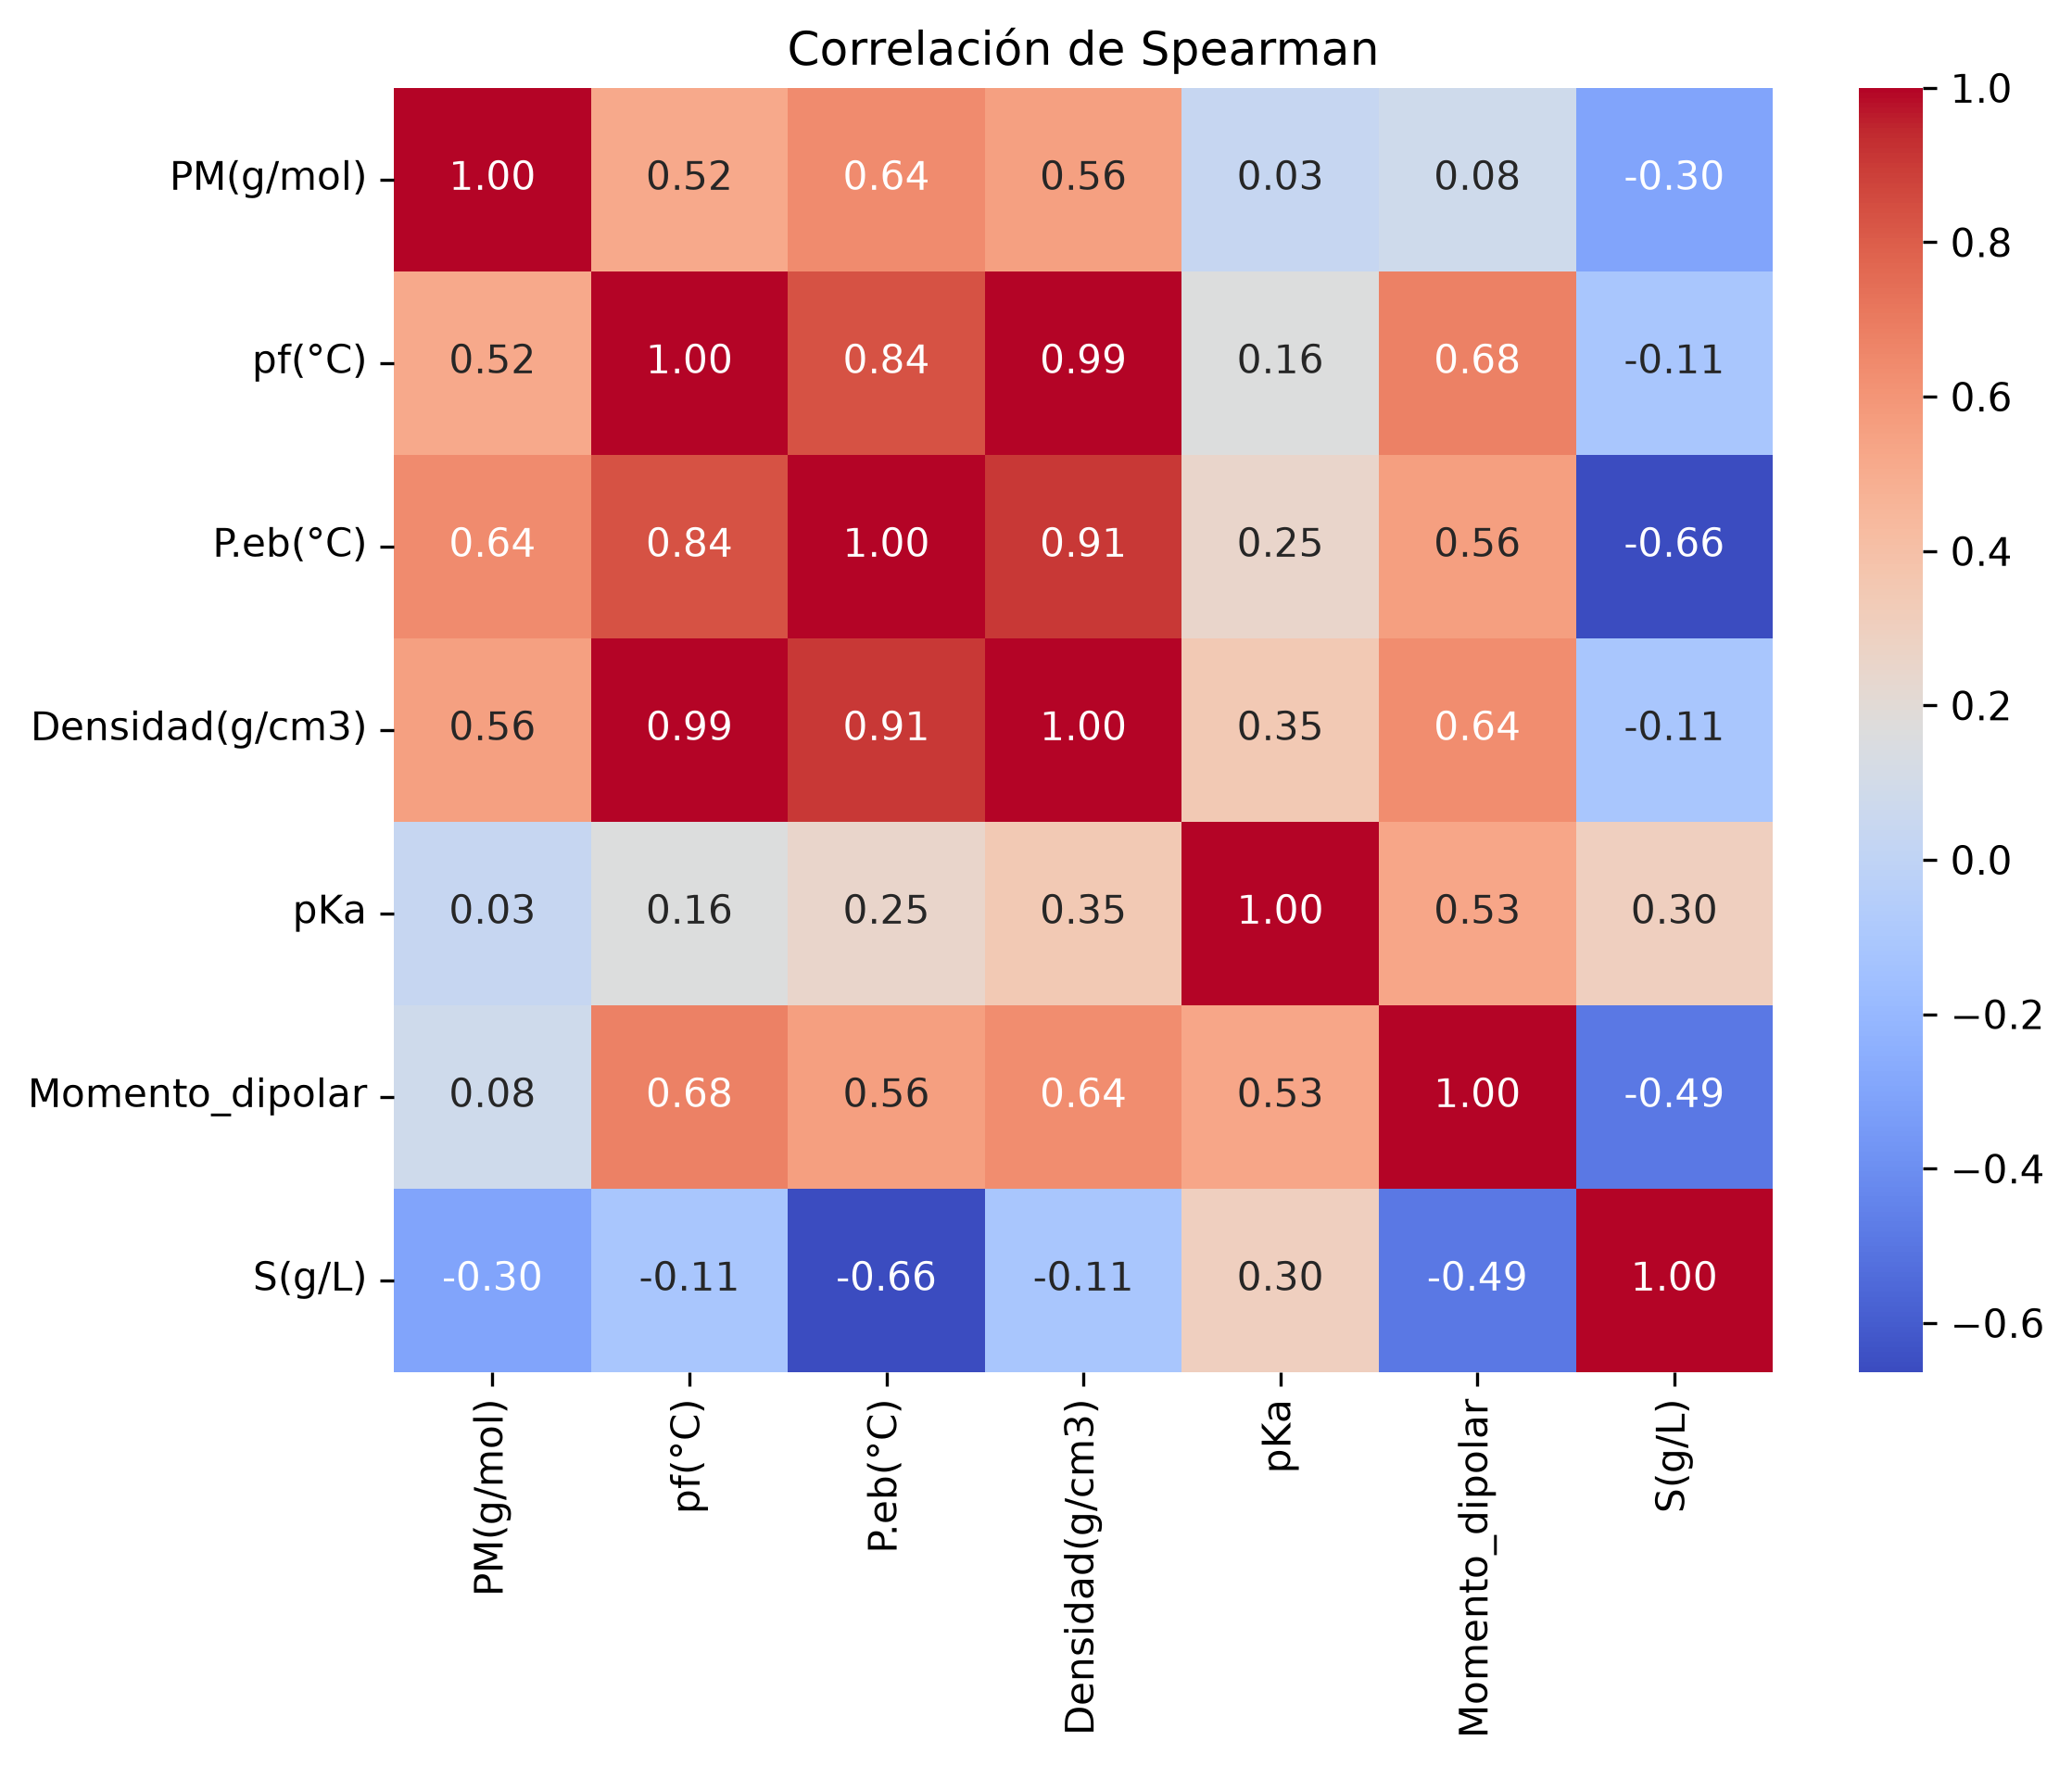
\includegraphics[width=\columnwidth]{01_heatmap_spearman.png}
	\caption{Matriz de correlación de Spearman entre las propiedades fisicoquímicas.}
	\label{fig:heatmap}
\end{figure}

\begin{figure}[htbp]
	\centering
	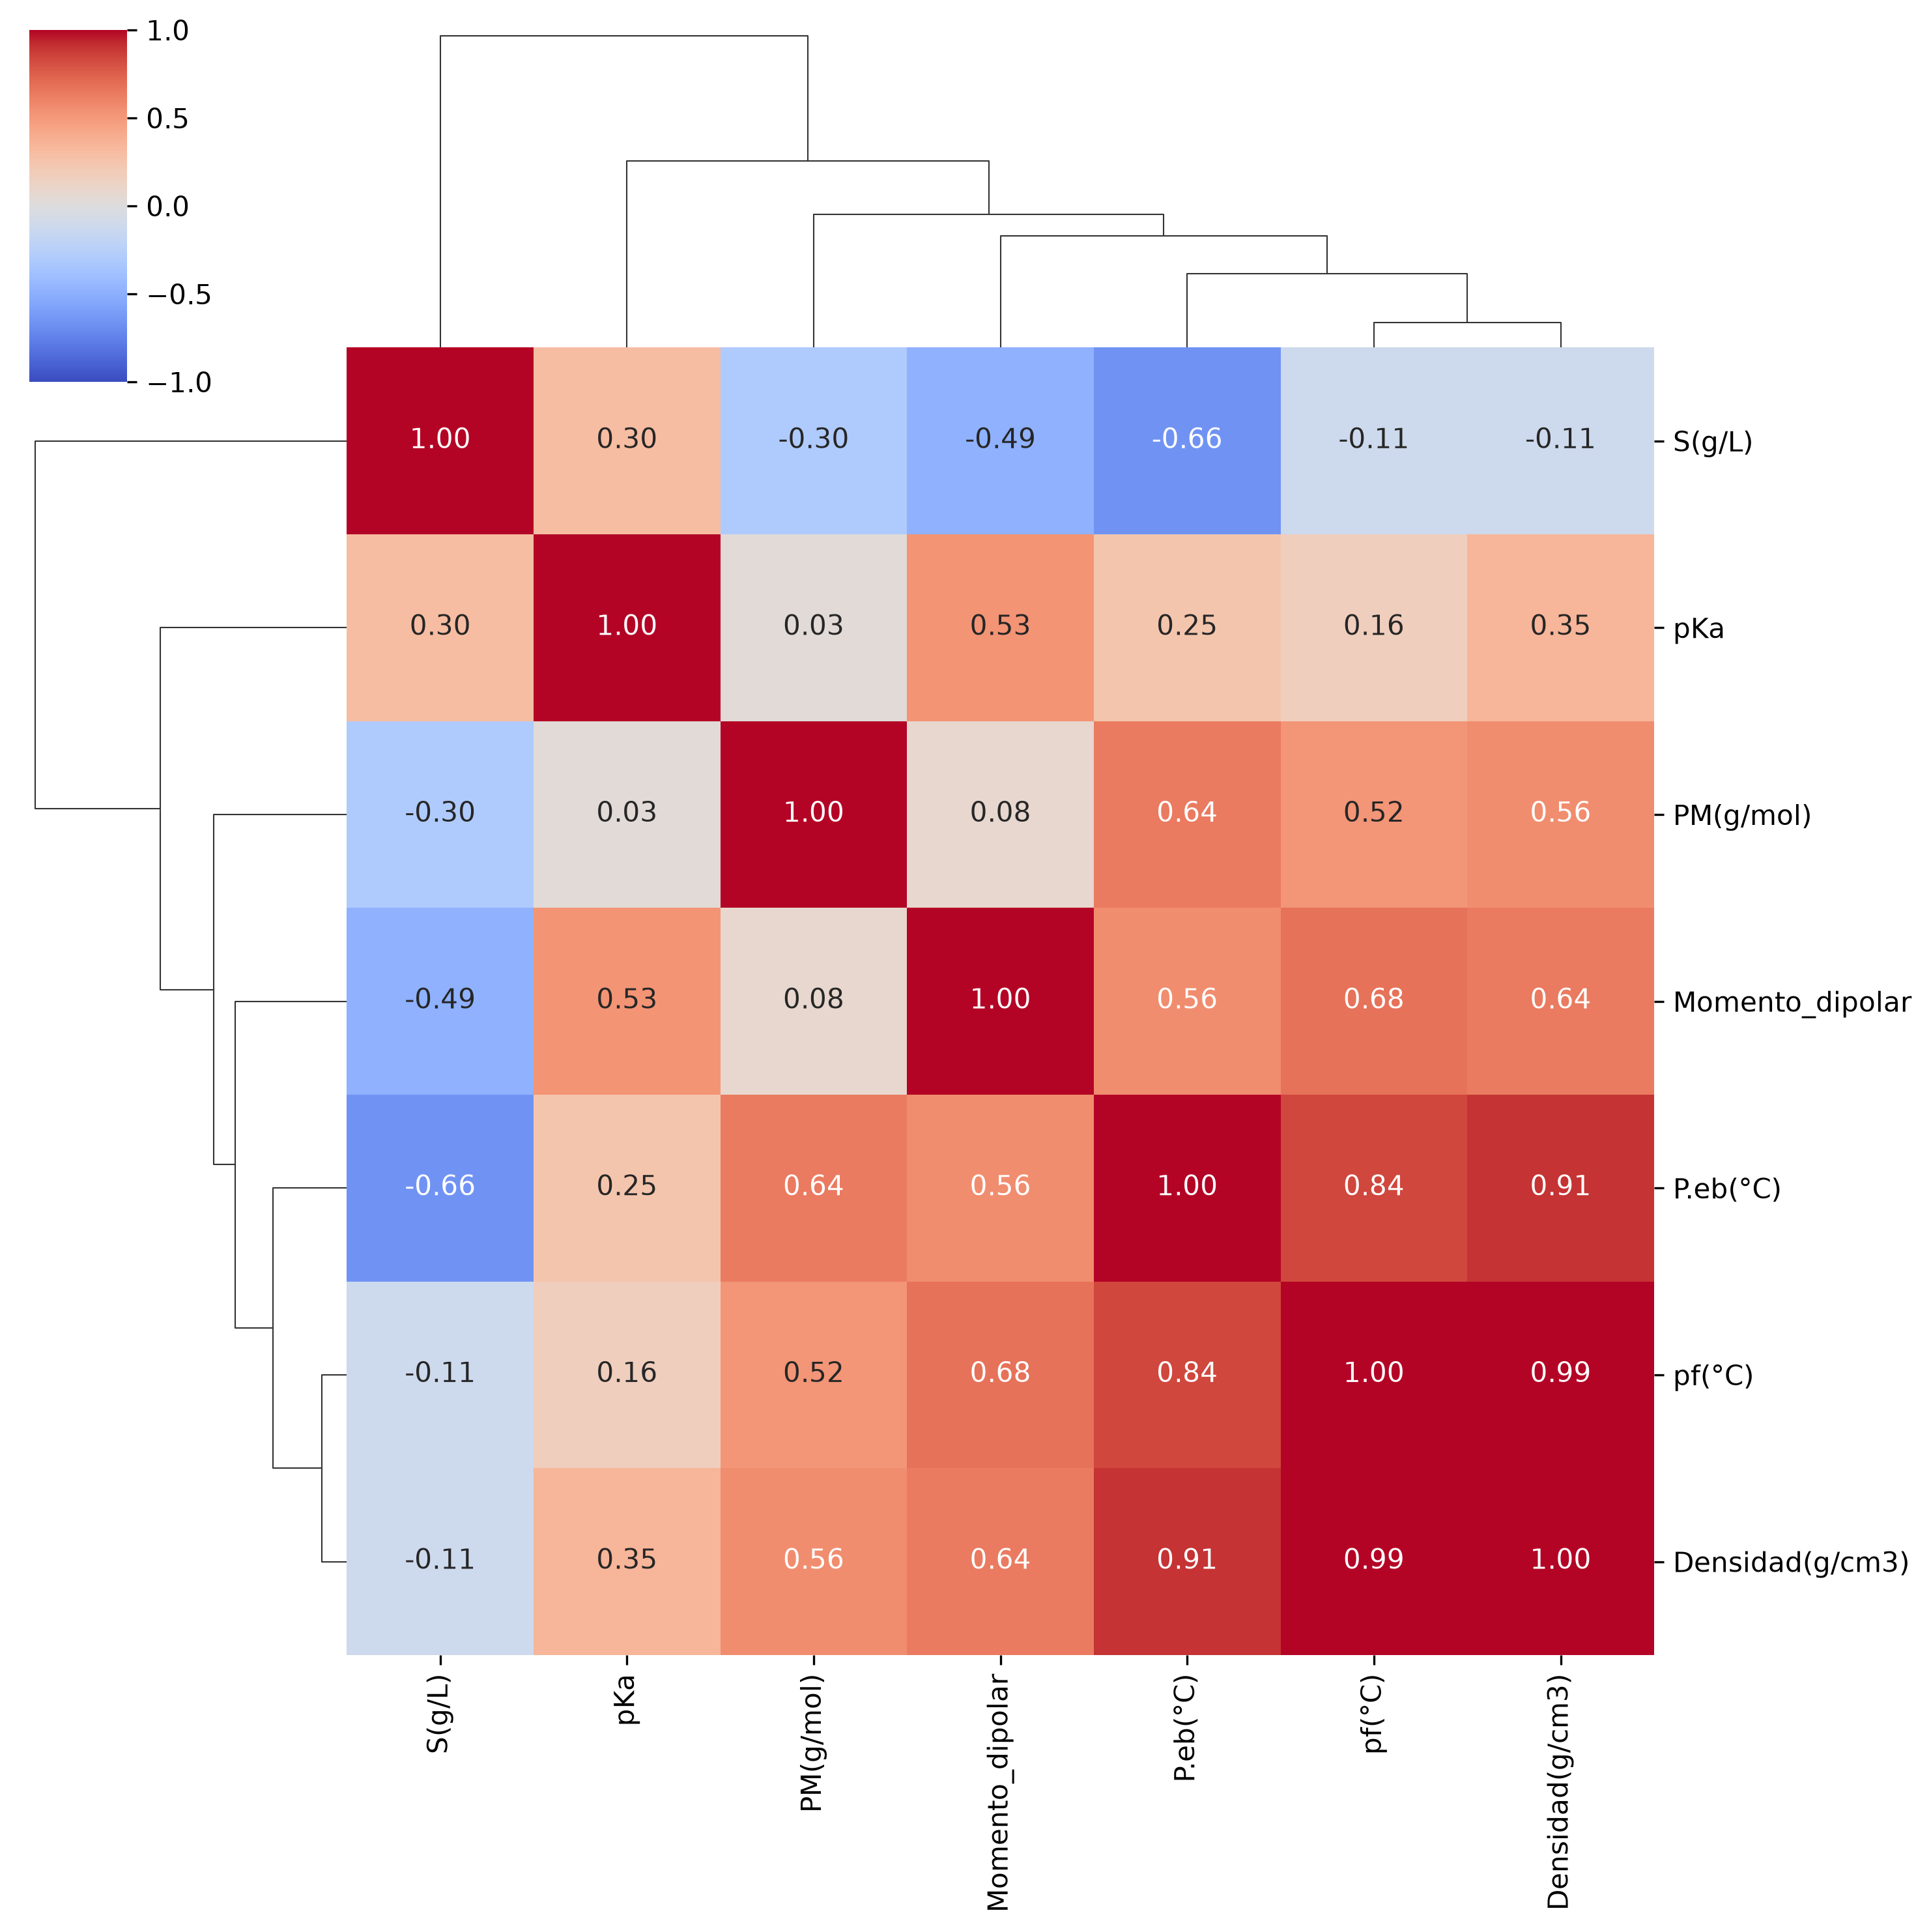
\includegraphics[width=\columnwidth]{02_clustermap_spearman.png}
	\caption{Mapa de agrupamiento jerárquico de la correlación de Spearman.}
	\label{fig:clustermap}
\end{figure}

\subsection{Tendencias entre propiedades}
% TODO (Valentina): discutir cada regresión en términos de fuerzas intermoleculares.
Las Figuras~\ref{fig:pf-dens}--\ref{fig:dip-peb} muestran las regresiones
lineales entre pares de propiedades, con su intervalo de confianza.
\textit{[Interpretación pendiente.]}

\begin{figure}[htbp]
	\centering
	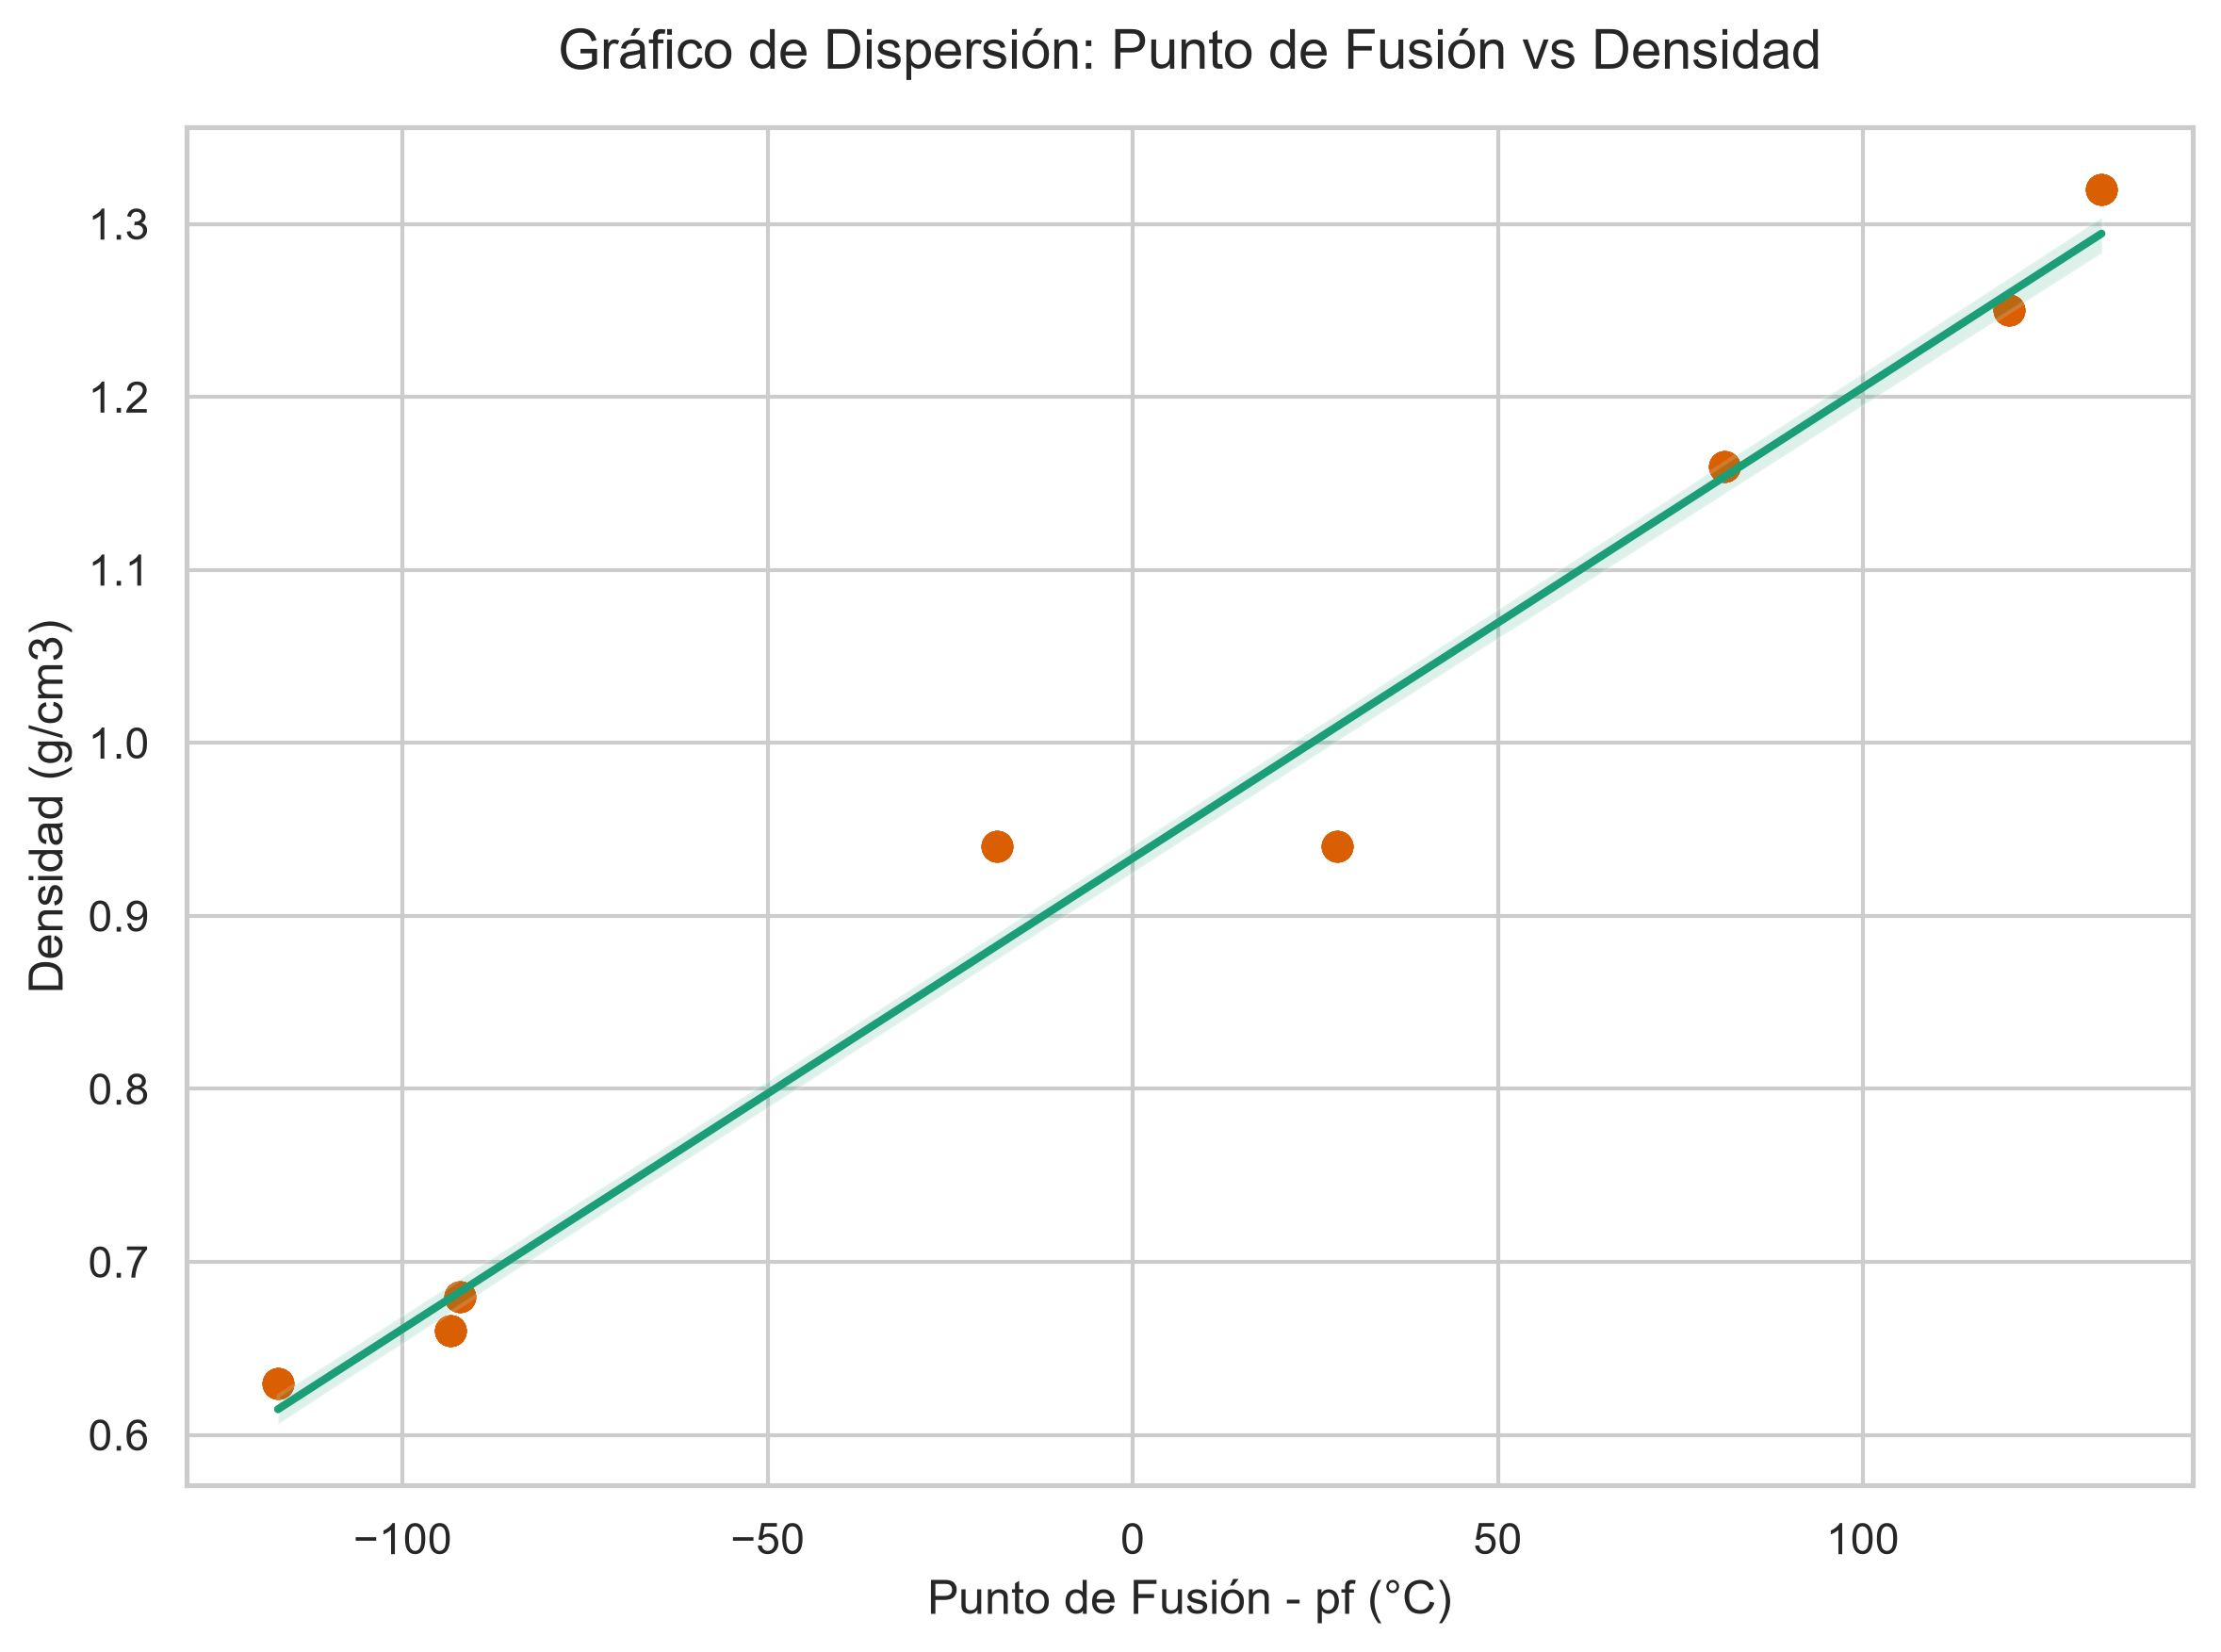
\includegraphics[width=\columnwidth]{03_reg_pf_vs_densidad.png}
	\caption{Punto de fusión frente a densidad.}
	\label{fig:pf-dens}
\end{figure}

\begin{figure}[htbp]
	\centering
	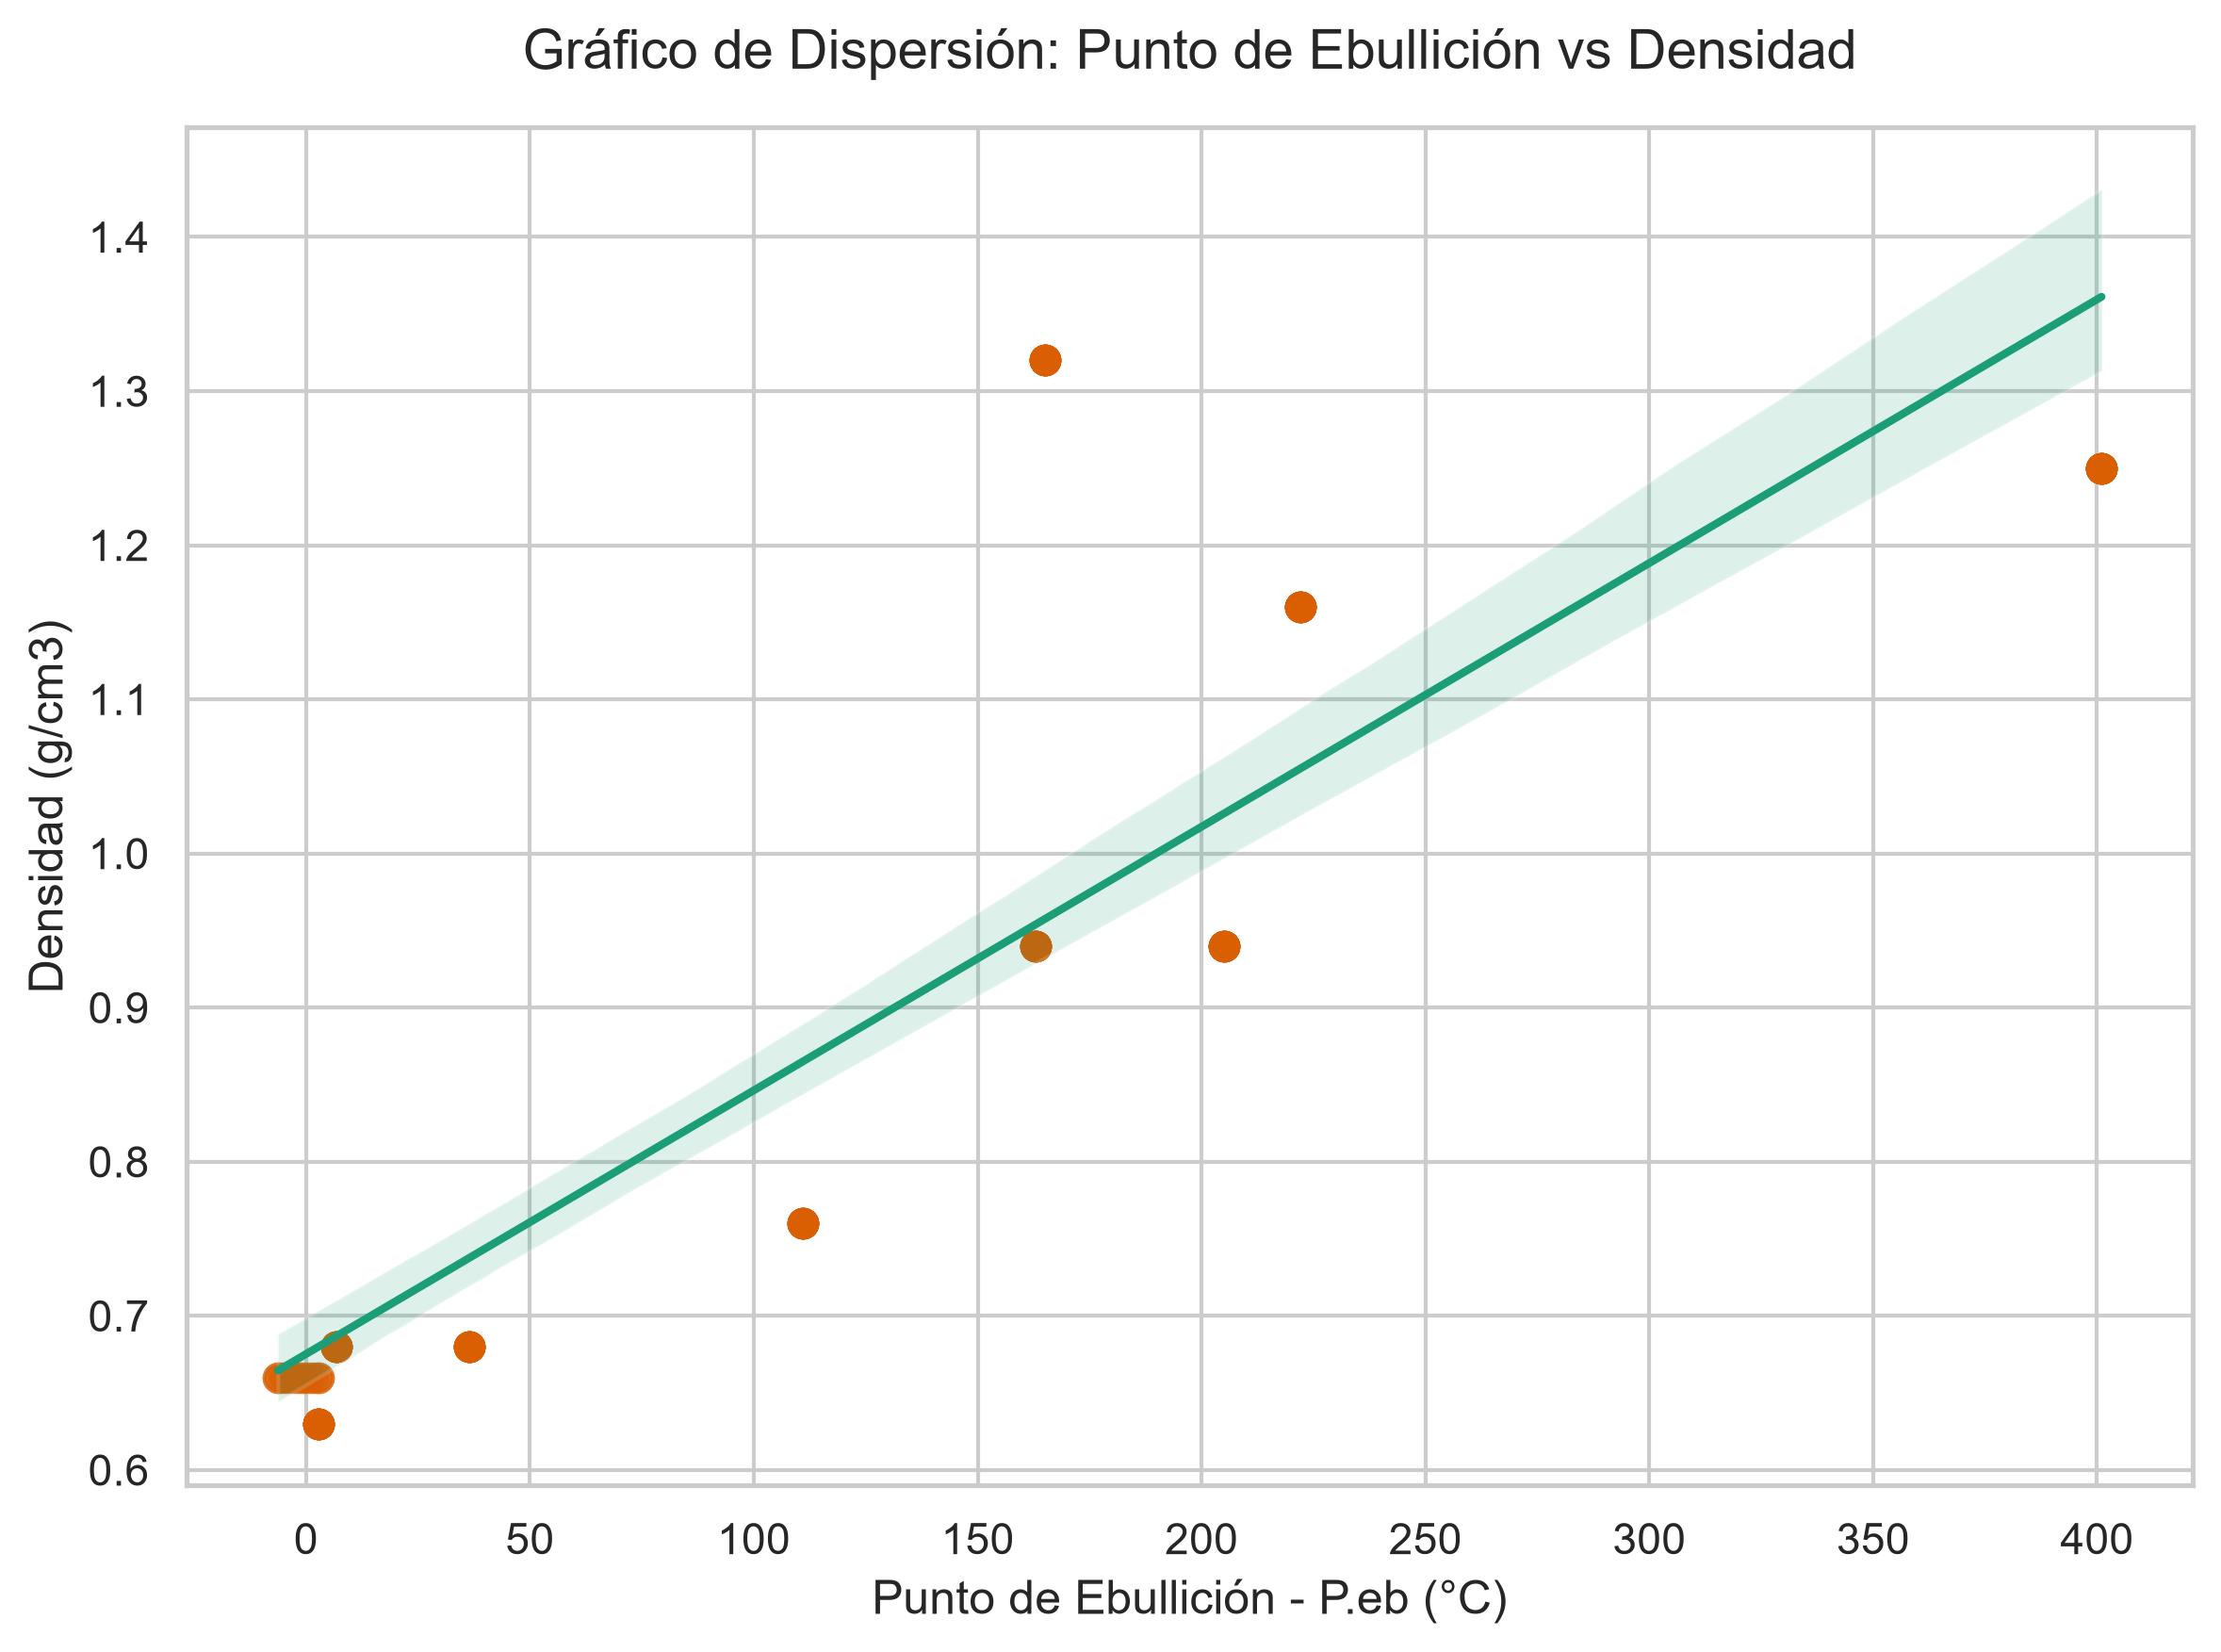
\includegraphics[width=\columnwidth]{04_reg_peb_vs_densidad.png}
	\caption{Punto de ebullición frente a densidad.}
	\label{fig:peb-dens}
\end{figure}

\begin{figure}[htbp]
	\centering
	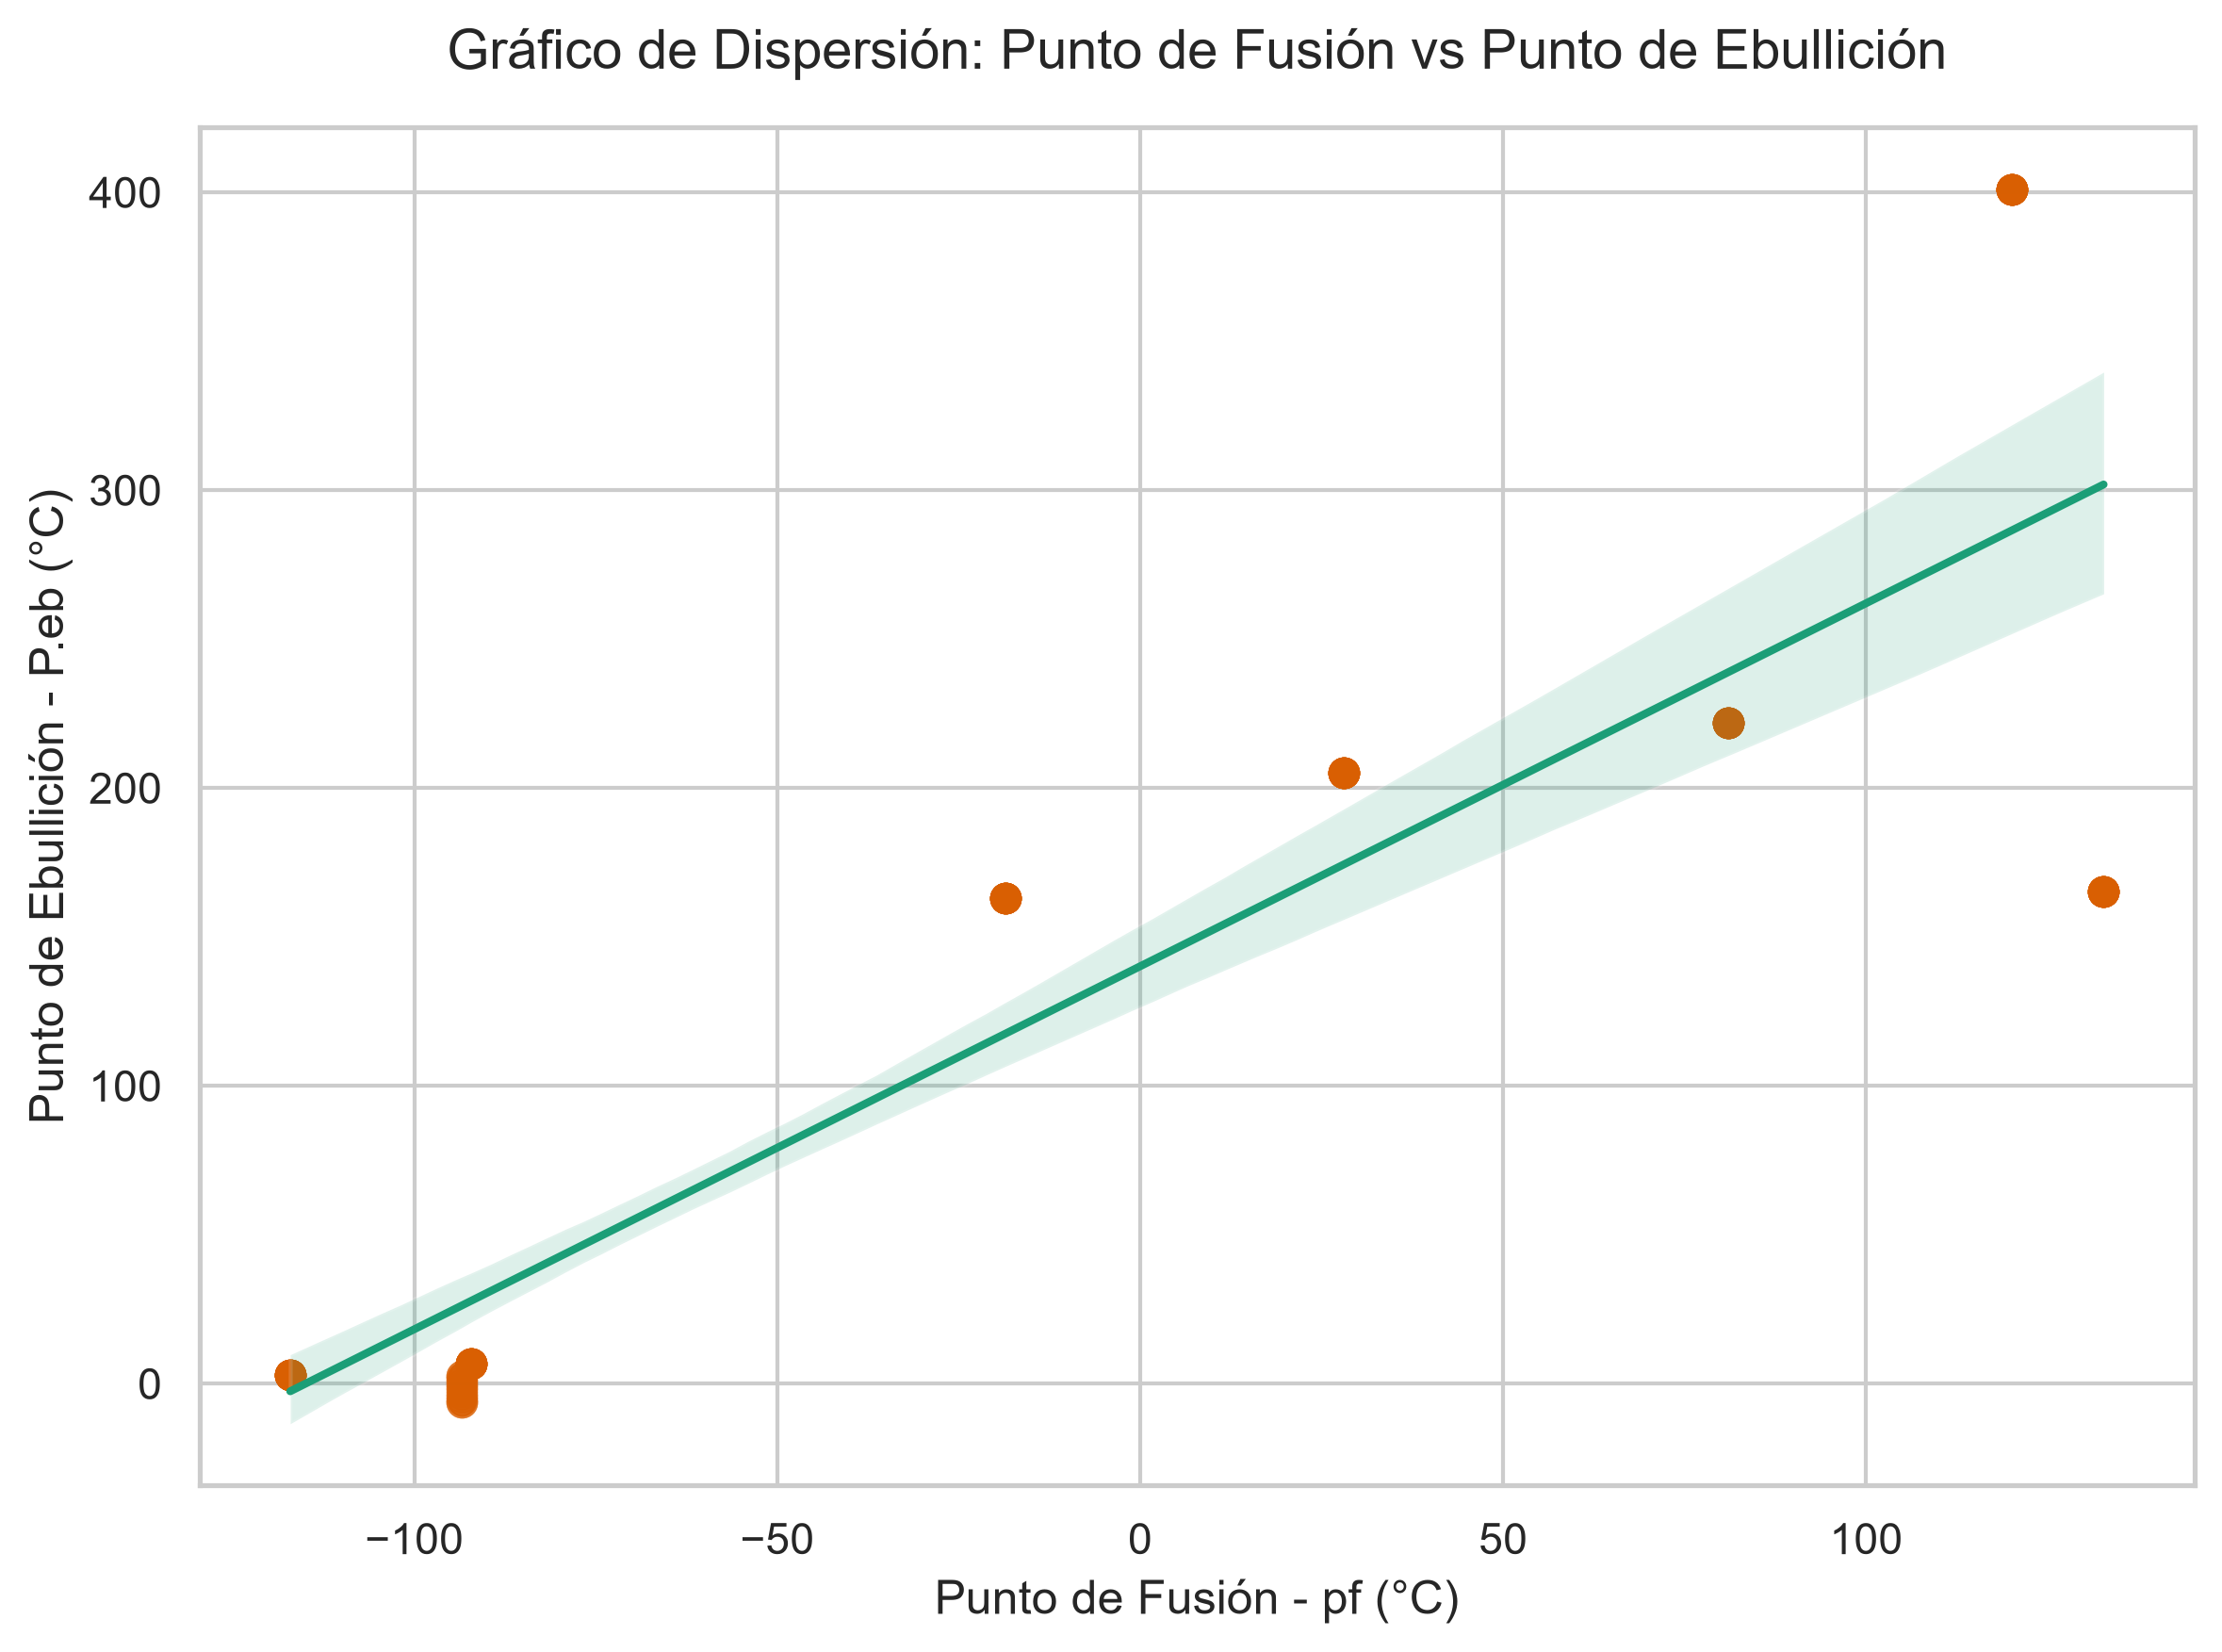
\includegraphics[width=\columnwidth]{05_reg_pf_vs_peb.png}
	\caption{Punto de fusión frente a punto de ebullición.}
	\label{fig:pf-peb}
\end{figure}

\begin{figure}[htbp]
	\centering
	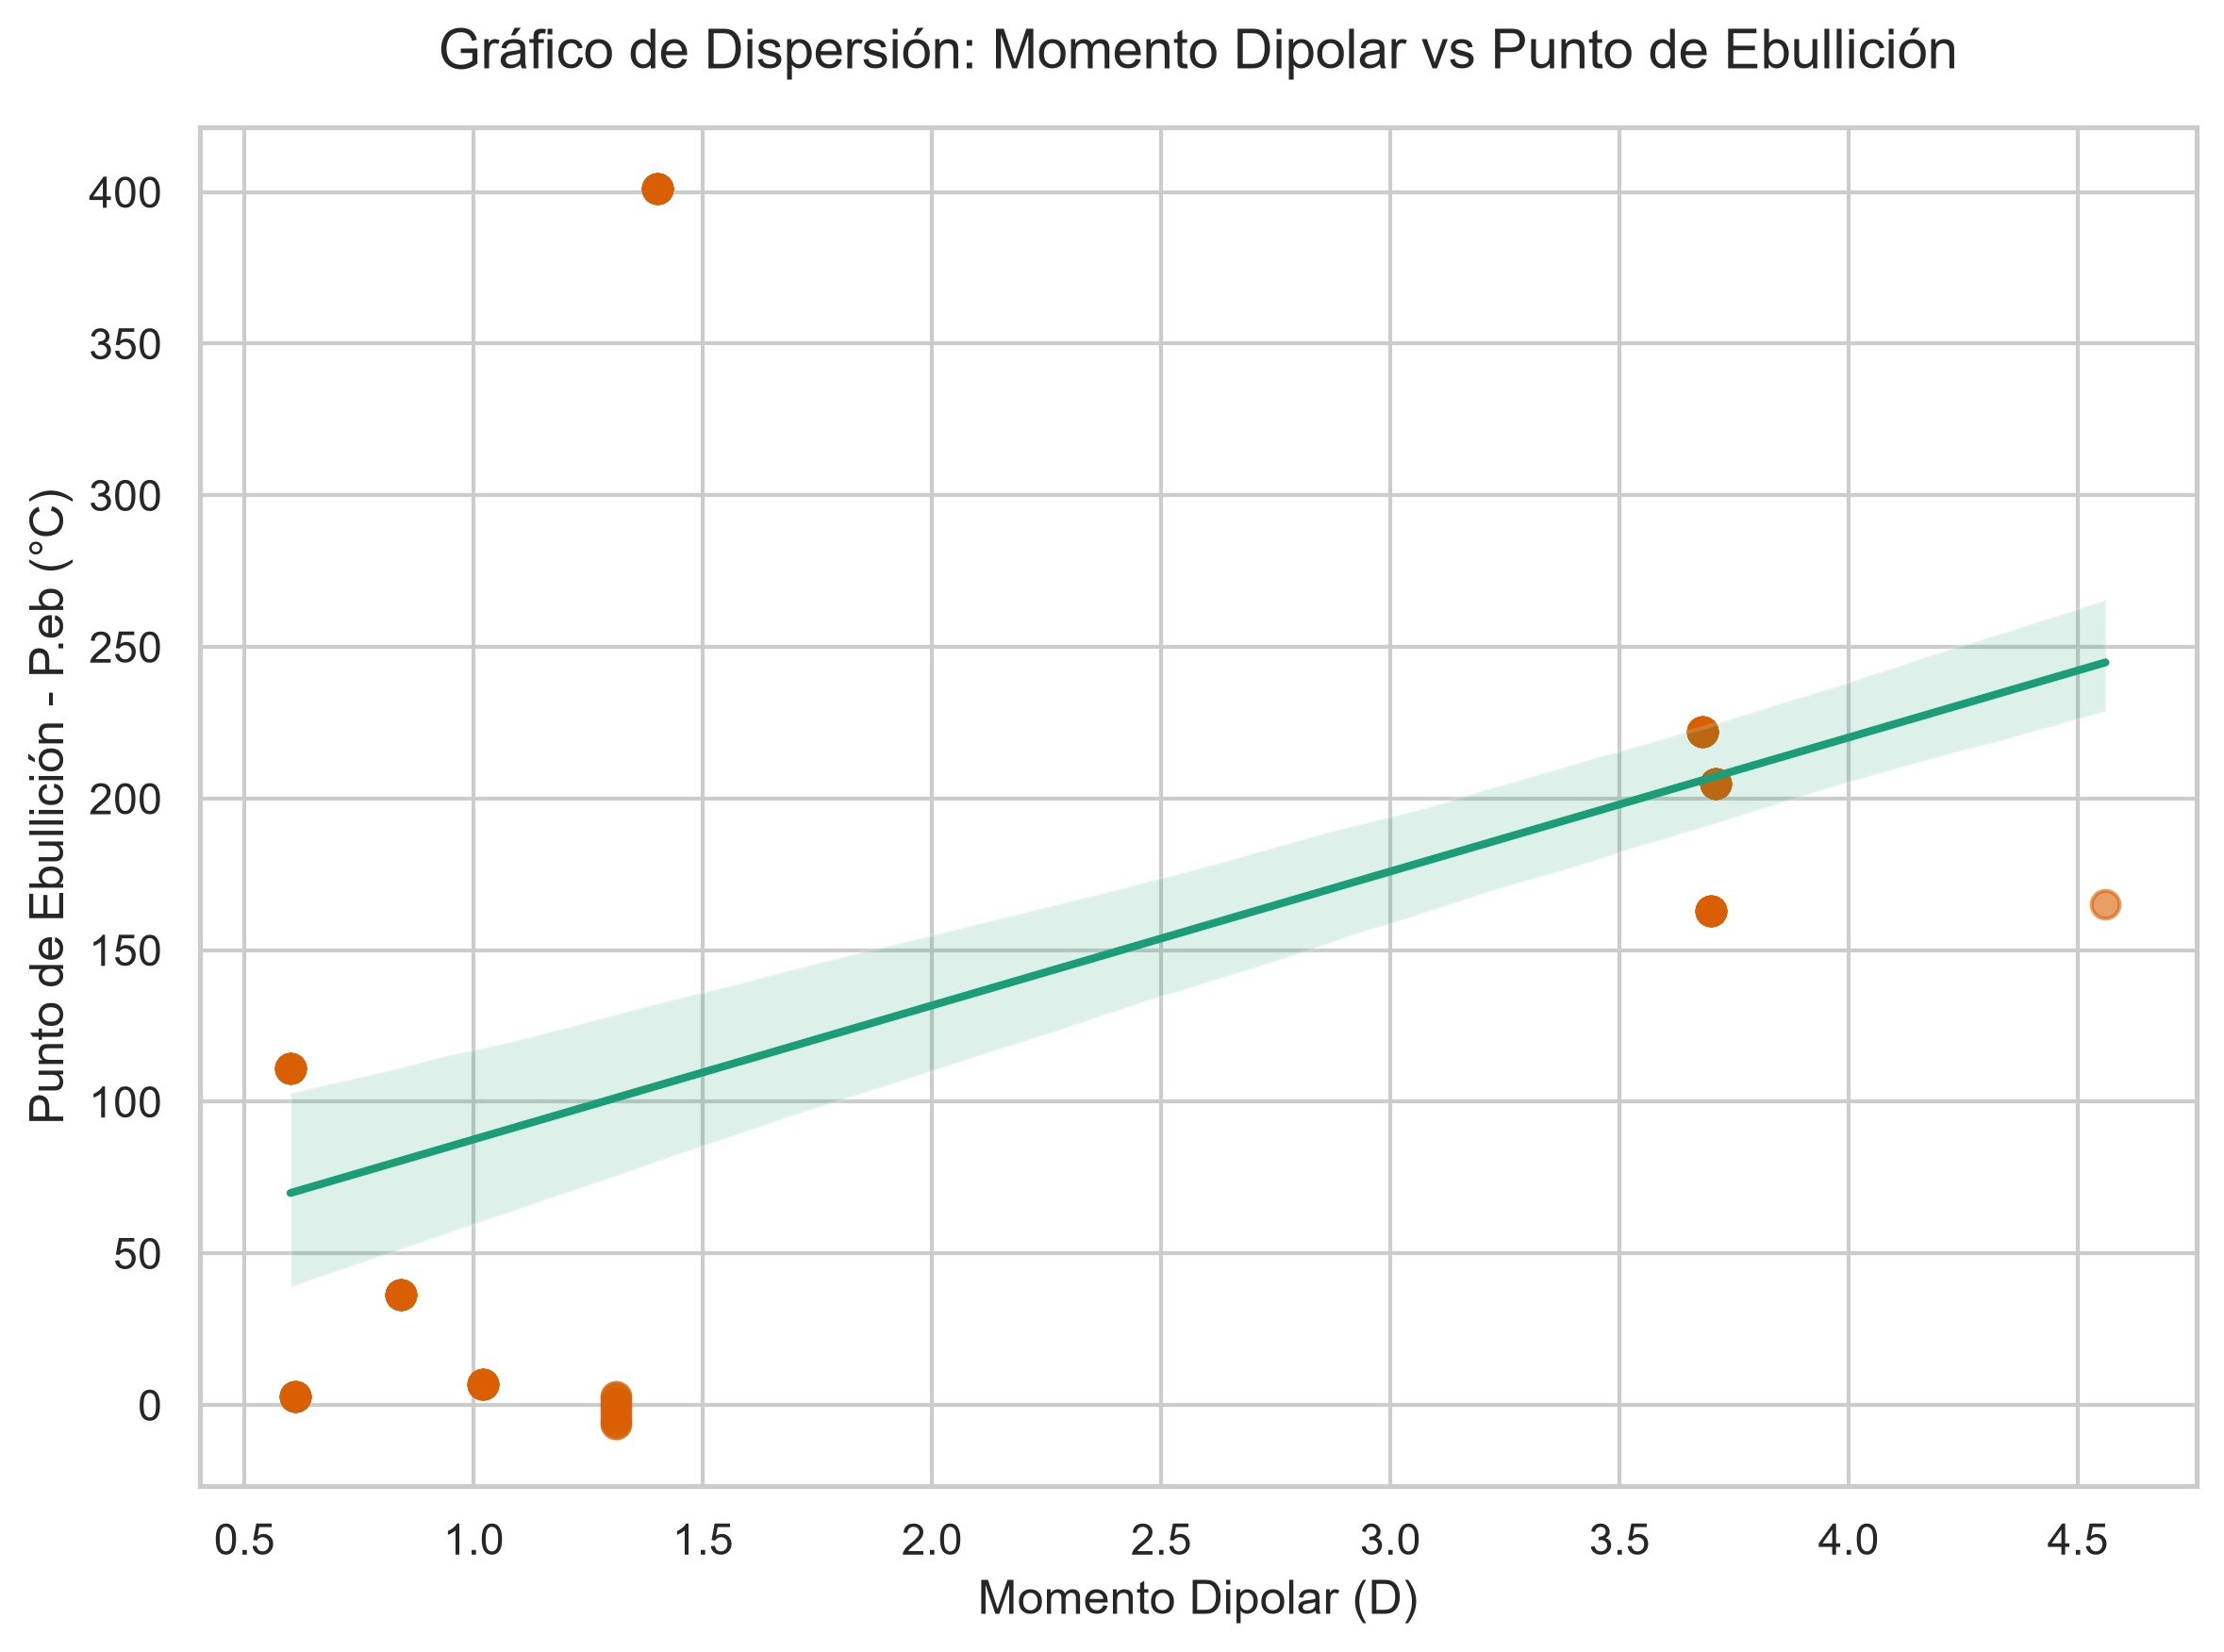
\includegraphics[width=\columnwidth]{06_reg_dipolo_vs_peb.png}
	\caption{Momento dipolar frente a punto de ebullición.}
	\label{fig:dip-peb}
\end{figure}

\subsection{Exploración interactiva con Plotly}
% TODO (Valentina): interpretar; idea central: a igual PM, los compuestos con
% enlace N--H (donadores de puente de H) hierven mucho más alto.
Las Figuras~\ref{fig:burbujas}--\ref{fig:dens-sol} se generaron con Plotly,
una fila por compuesto; sus versiones HTML permiten inspeccionar cada molécula
con el cursor. En la Figura~\ref{fig:burbujas}, trimetilamina
(\SI{2.8}{\degreeCelsius}) y N-metiletanamina (\SI{36.5}{\degreeCelsius}) tienen
el mismo peso molecular (\SI{59.11}{\gram\per\mole}): la diferencia se debe a que
sólo la segunda posee enlace N--H y forma puentes de hidrógeno.
\textit{[Interpretación pendiente.]}

\begin{figure}[htbp]
	\centering
	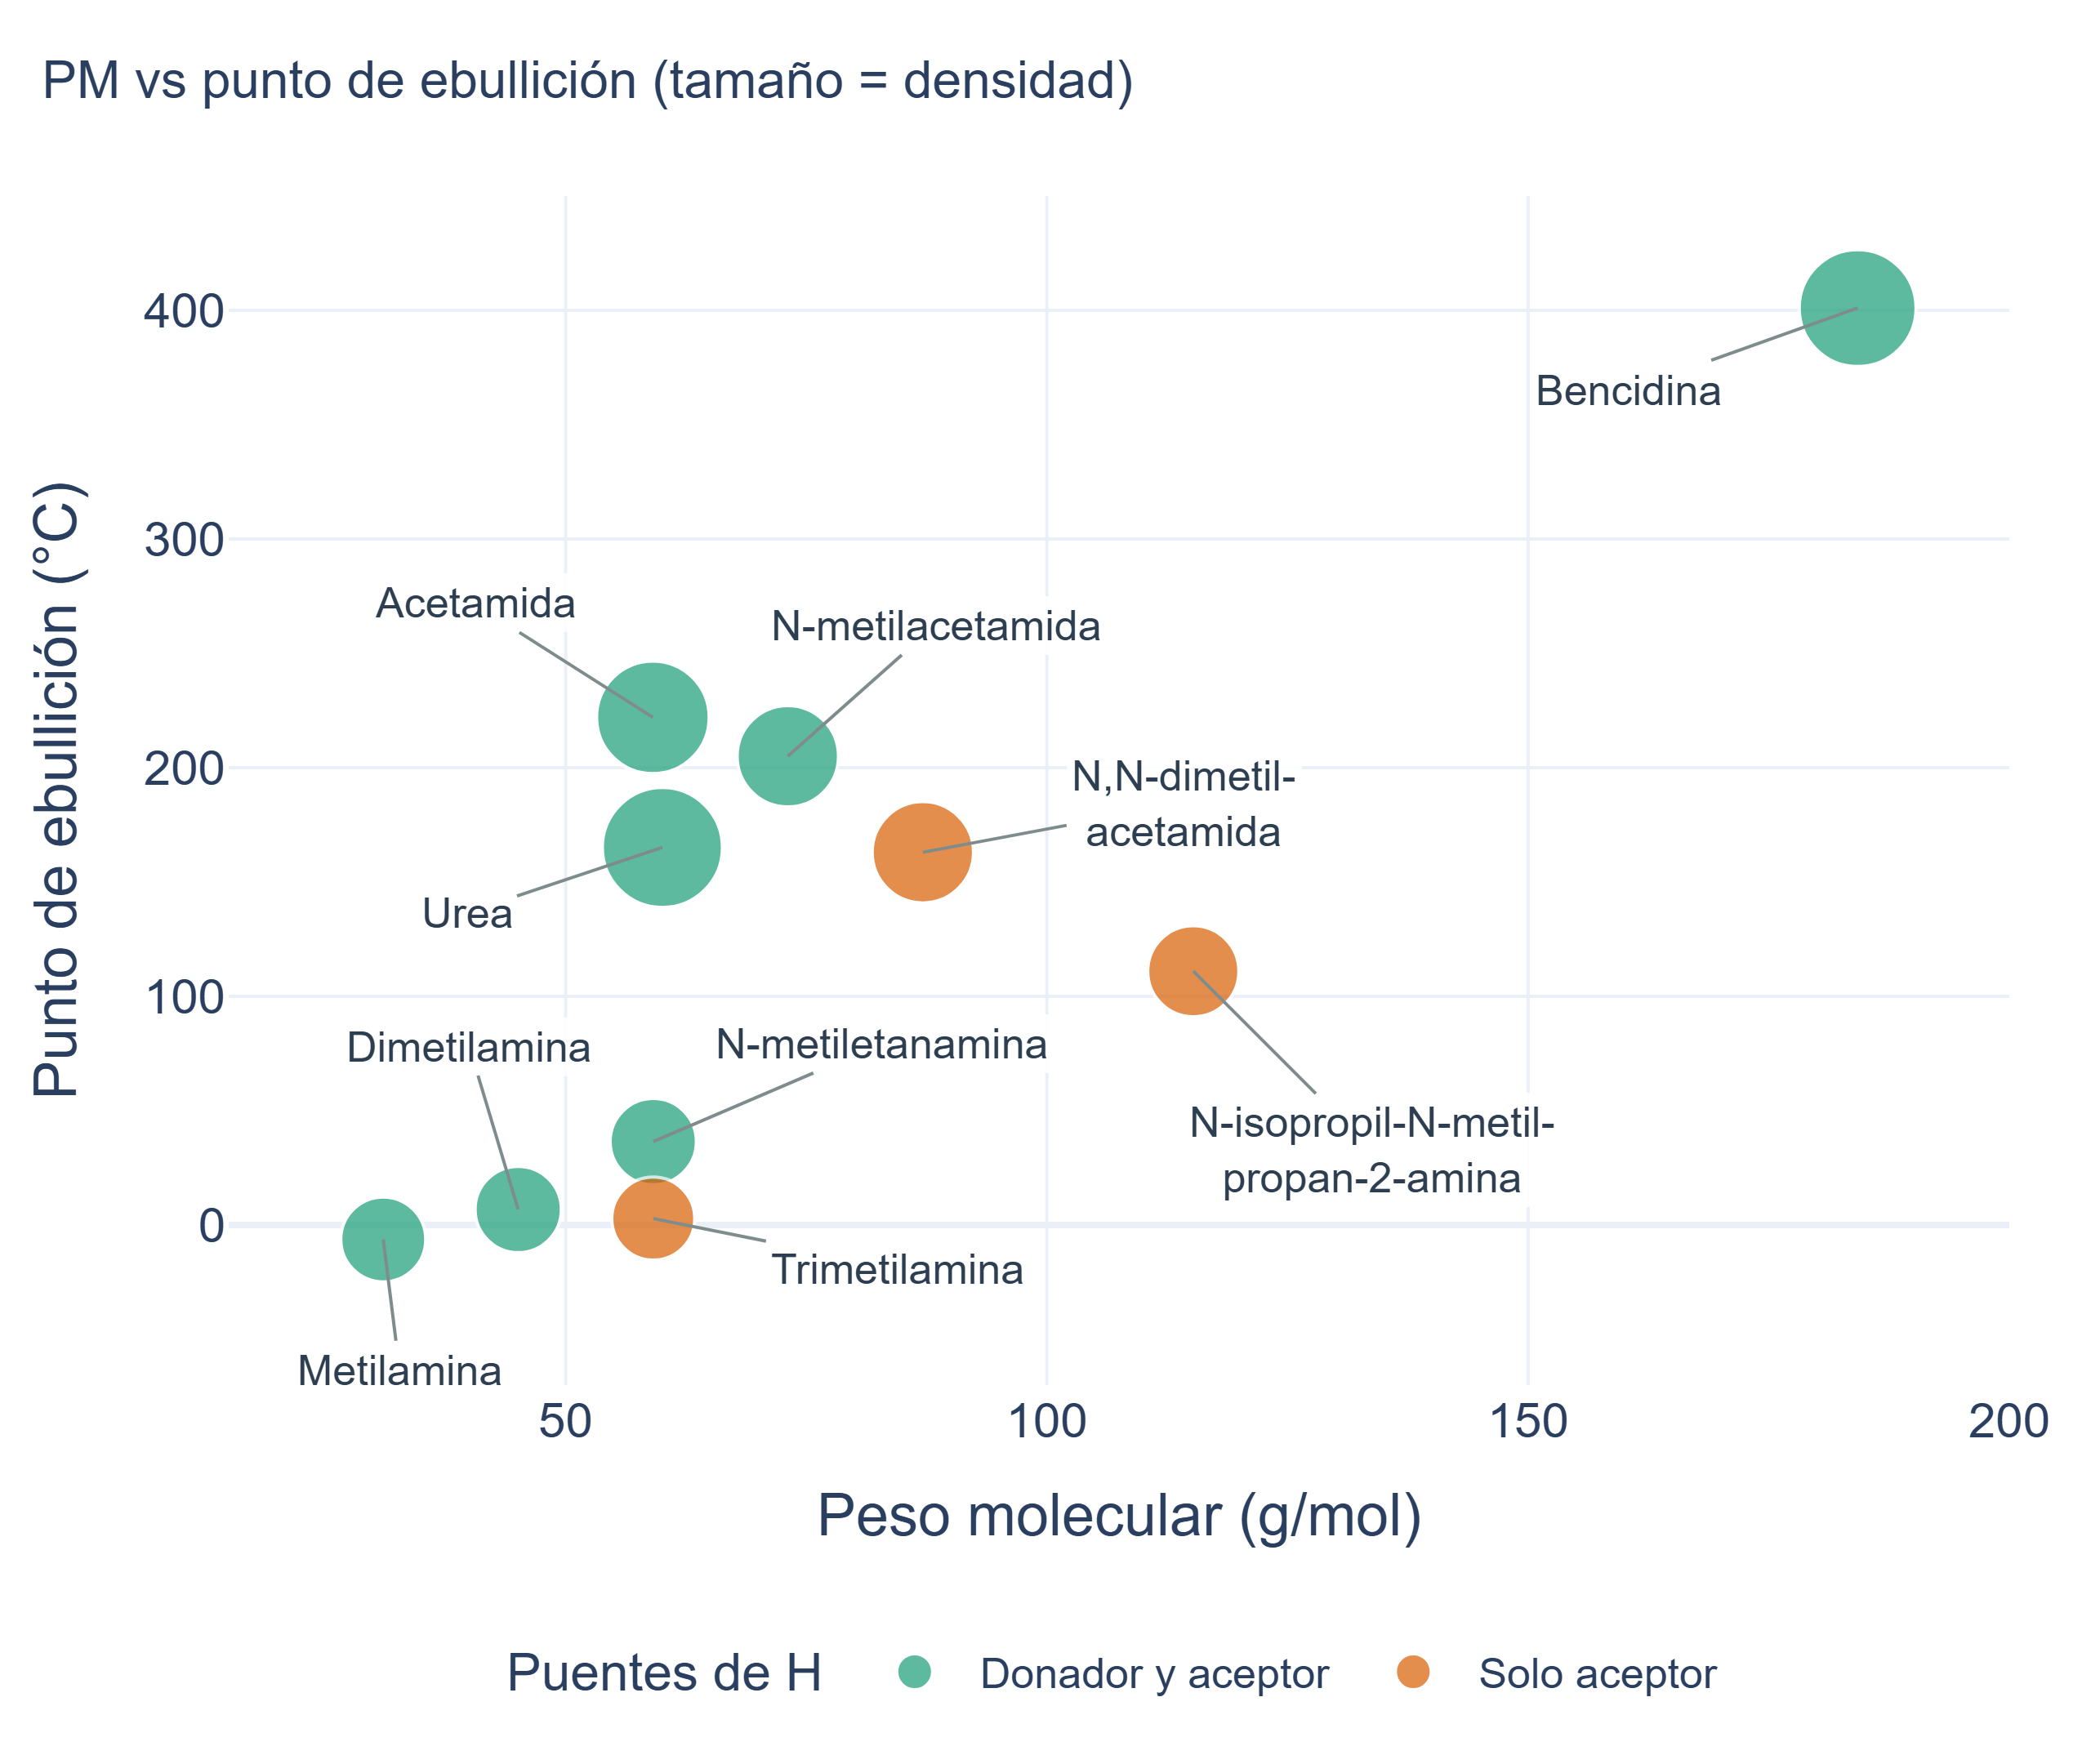
\includegraphics[width=\columnwidth]{11_plotly_burbujas_pm_peb.png}
	\caption{Peso molecular frente a punto de ebullición; el tamaño representa la densidad y el color la capacidad de formar puentes de hidrógeno.}
	\label{fig:burbujas}
\end{figure}

\begin{figure}[htbp]
	\centering
	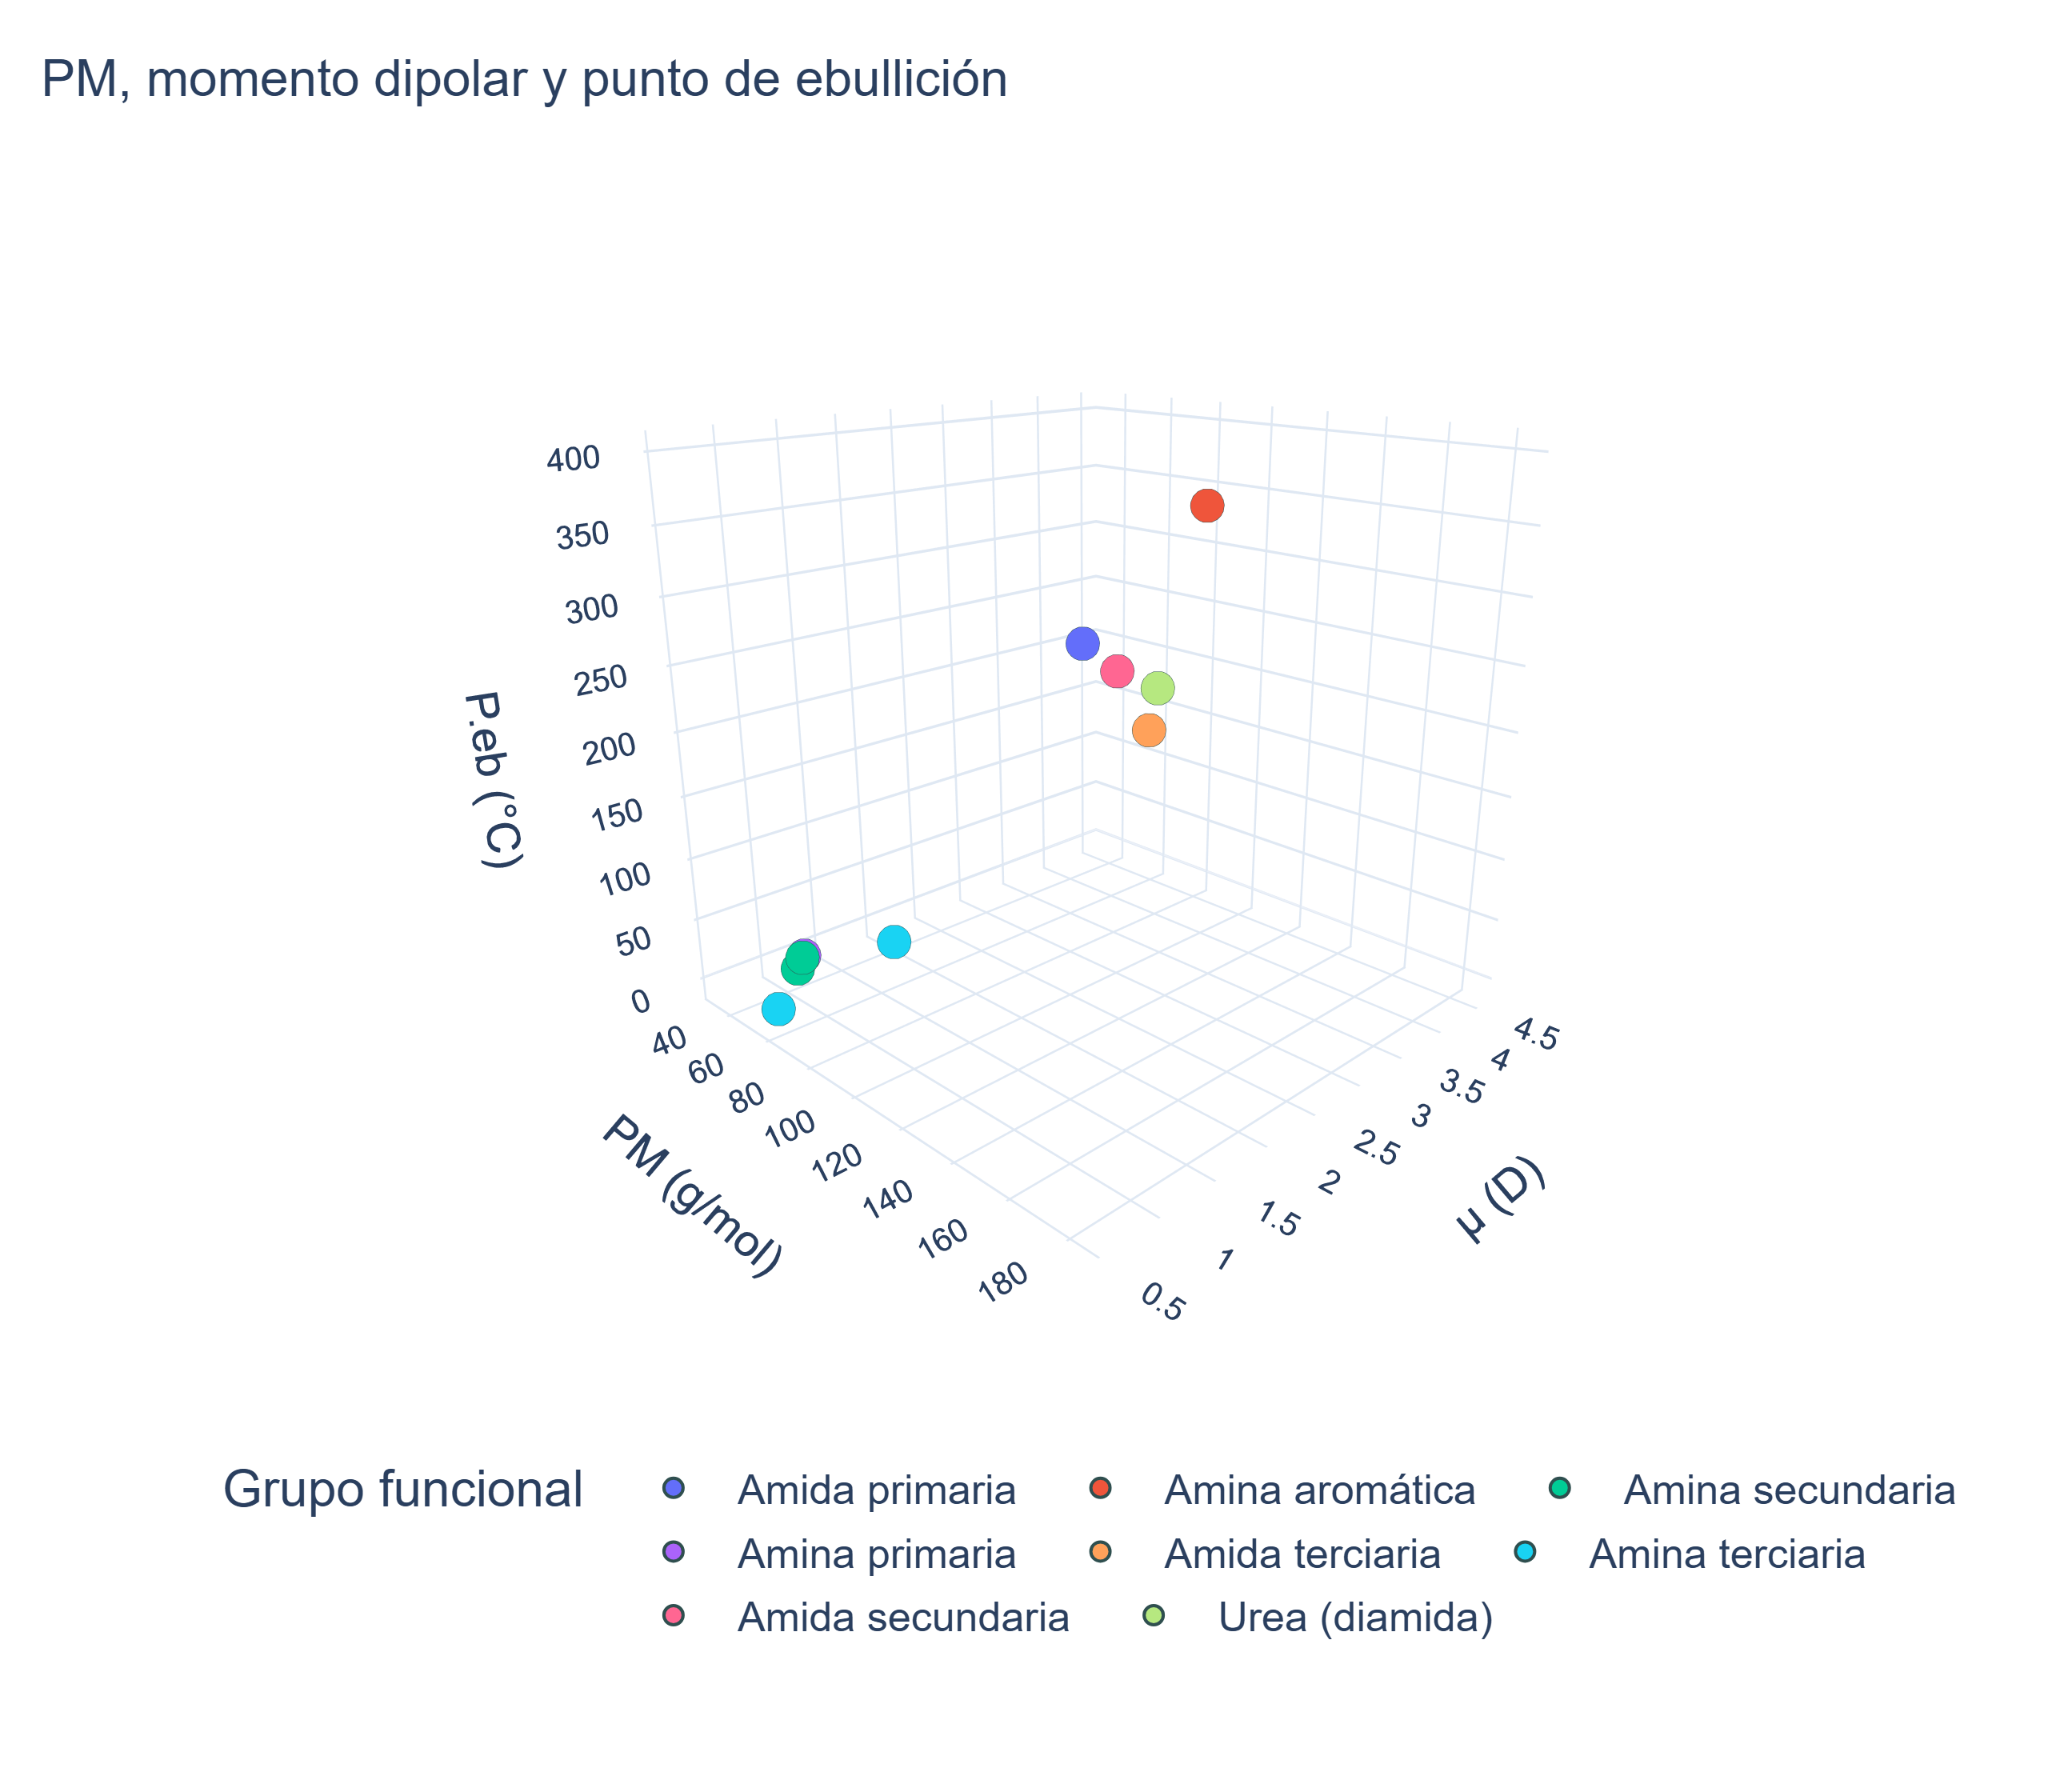
\includegraphics[width=\columnwidth]{12_plotly_3d_pm_dipolo_peb.png}
	\caption{Espacio tridimensional de peso molecular, momento dipolar y punto de ebullición por grupo funcional.}
	\label{fig:3d}
\end{figure}

\begin{figure}[htbp]
	\centering
	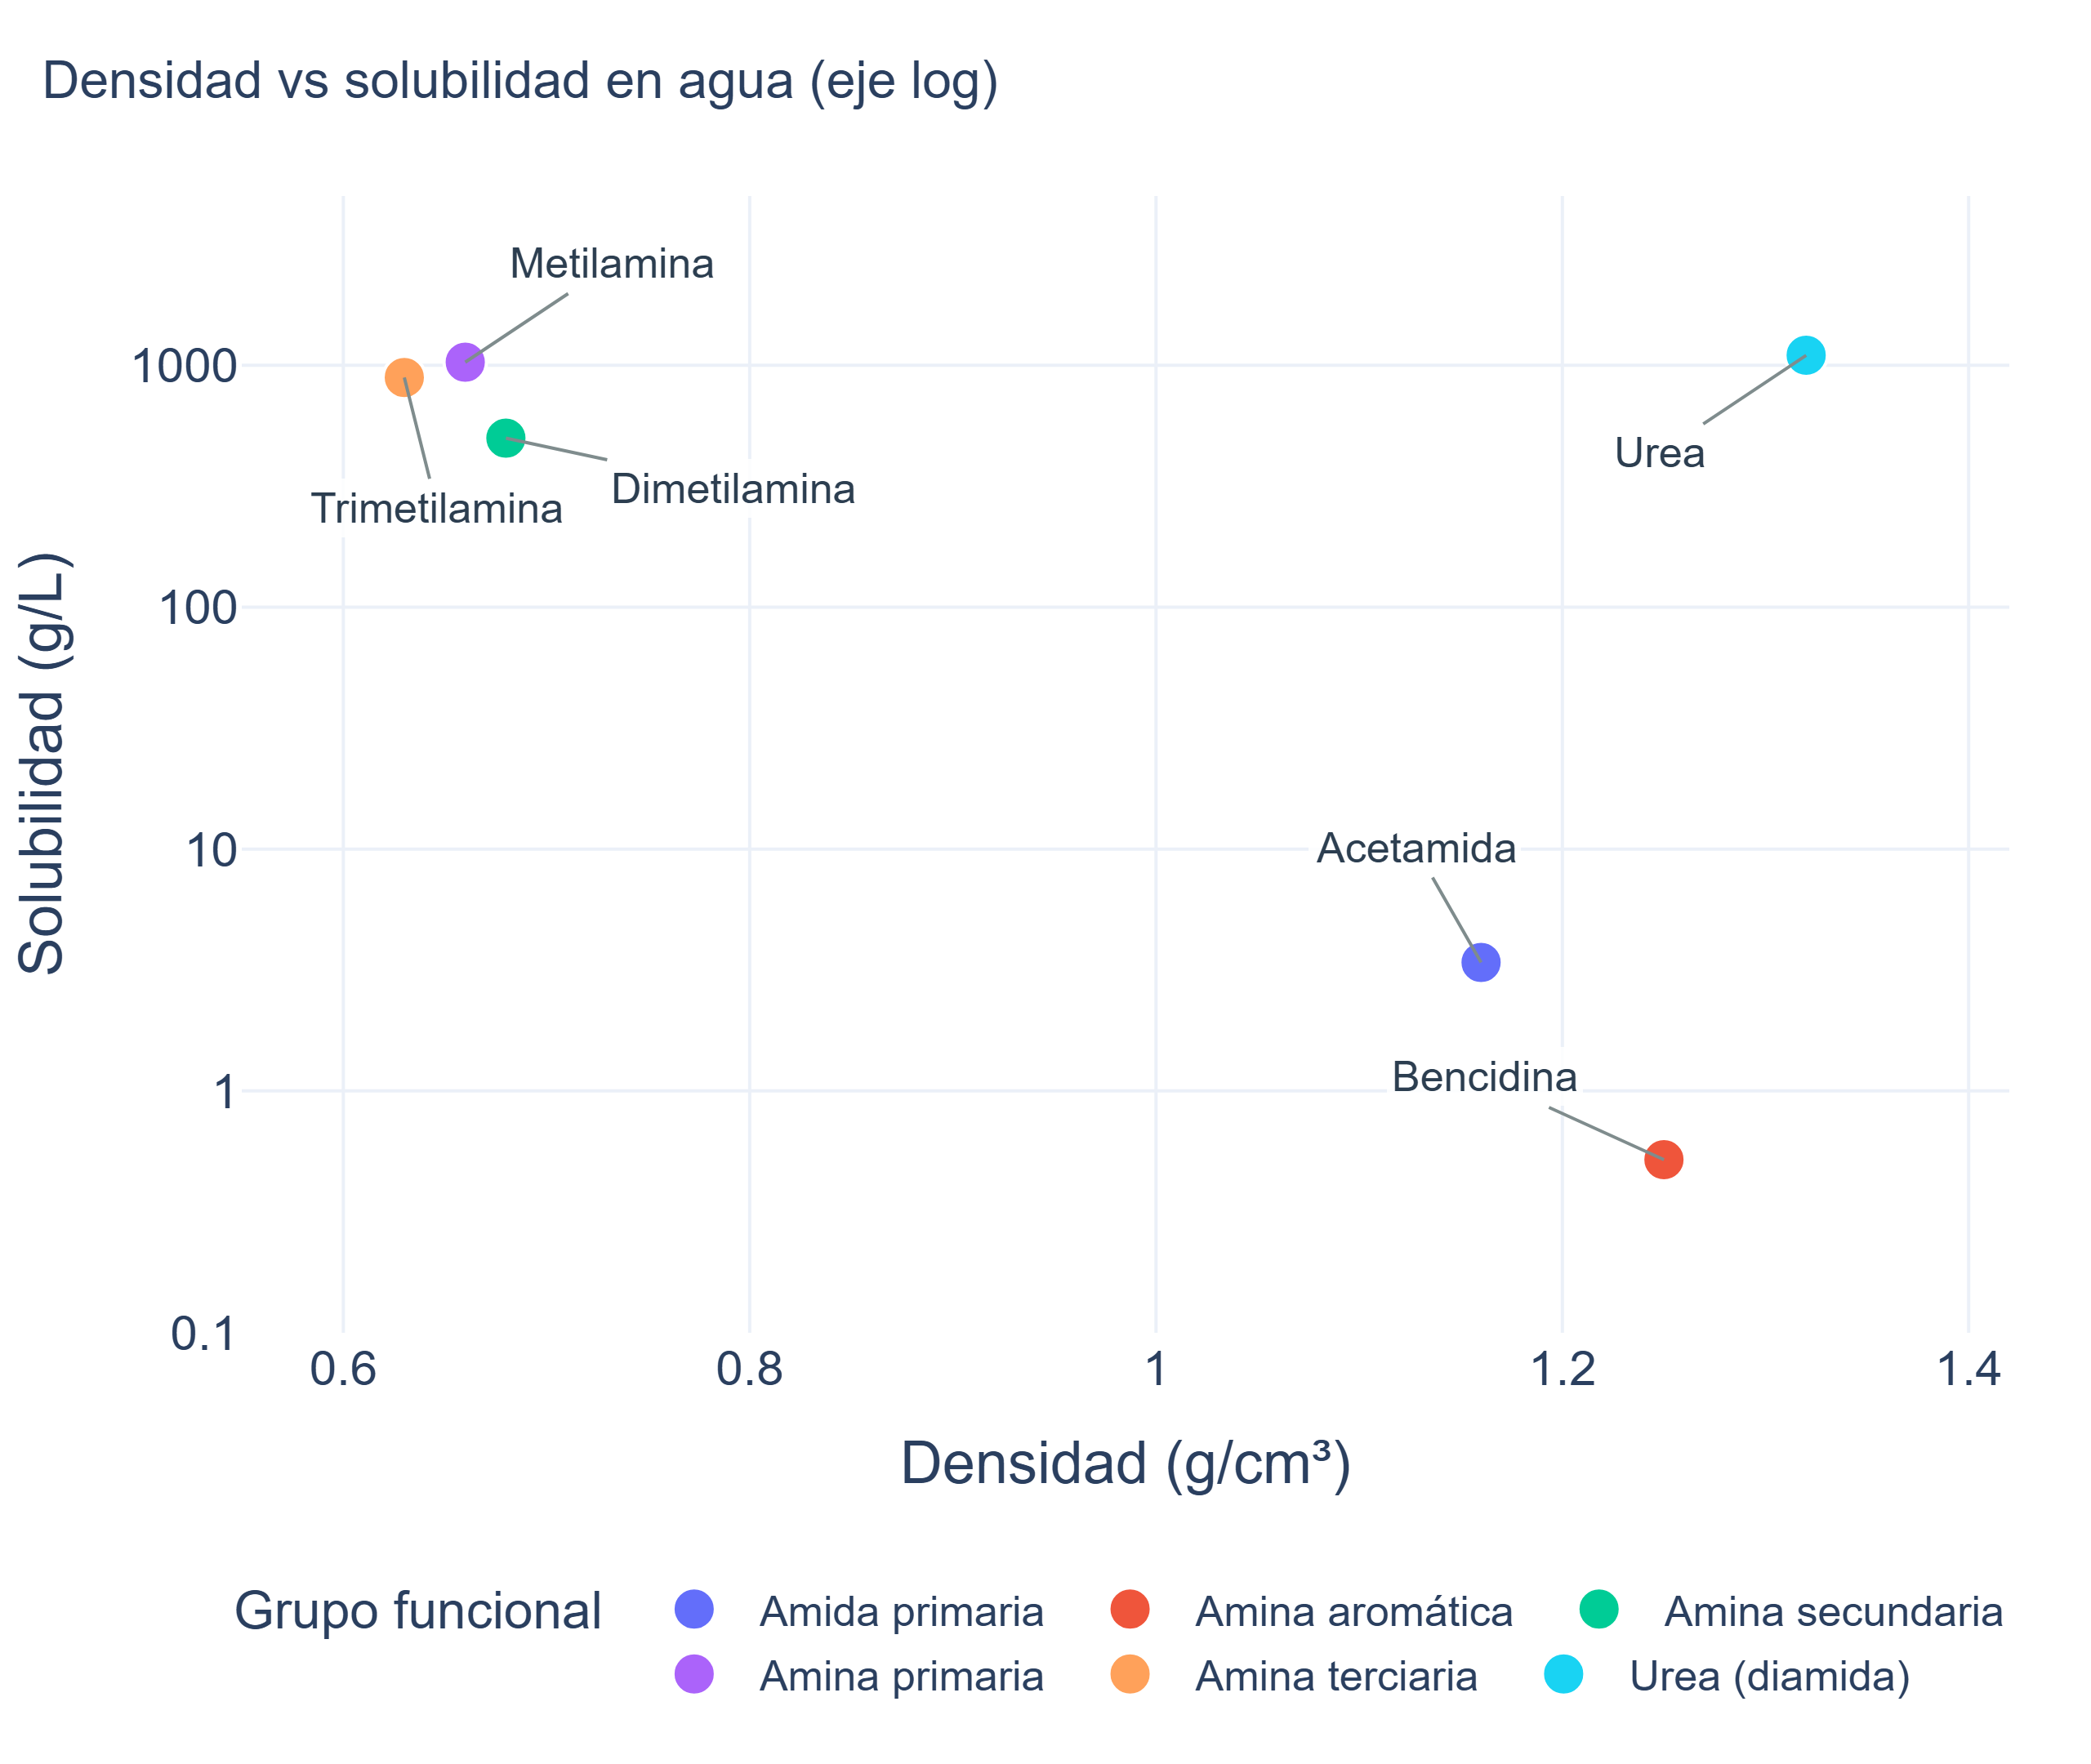
\includegraphics[width=\columnwidth]{13_plotly_densidad_solubilidad.png}
	\caption{Densidad frente a solubilidad en agua (eje logarítmico).}
	\label{fig:dens-sol}
\end{figure}

\subsection{Distribución por tipo de reacción y medio}
% TODO (Valentina): explicar qué representa TR y comparar medianas/dispersiones.
La Figura~\ref{fig:frecuencias} compara la frecuencia de cada mecanismo de
reacción y de cada medio; la sustitución nucleofílica (SN) domina, coherente con
el carácter nucleófilo del par libre del nitrógeno. Las
Figuras~\ref{fig:violin}--\ref{fig:dona} describen la distribución de
probabilidad de TR según el tipo de reacción y el medio.
\textit{[Interpretación pendiente.]}

\begin{figure}[htbp]
	\centering
	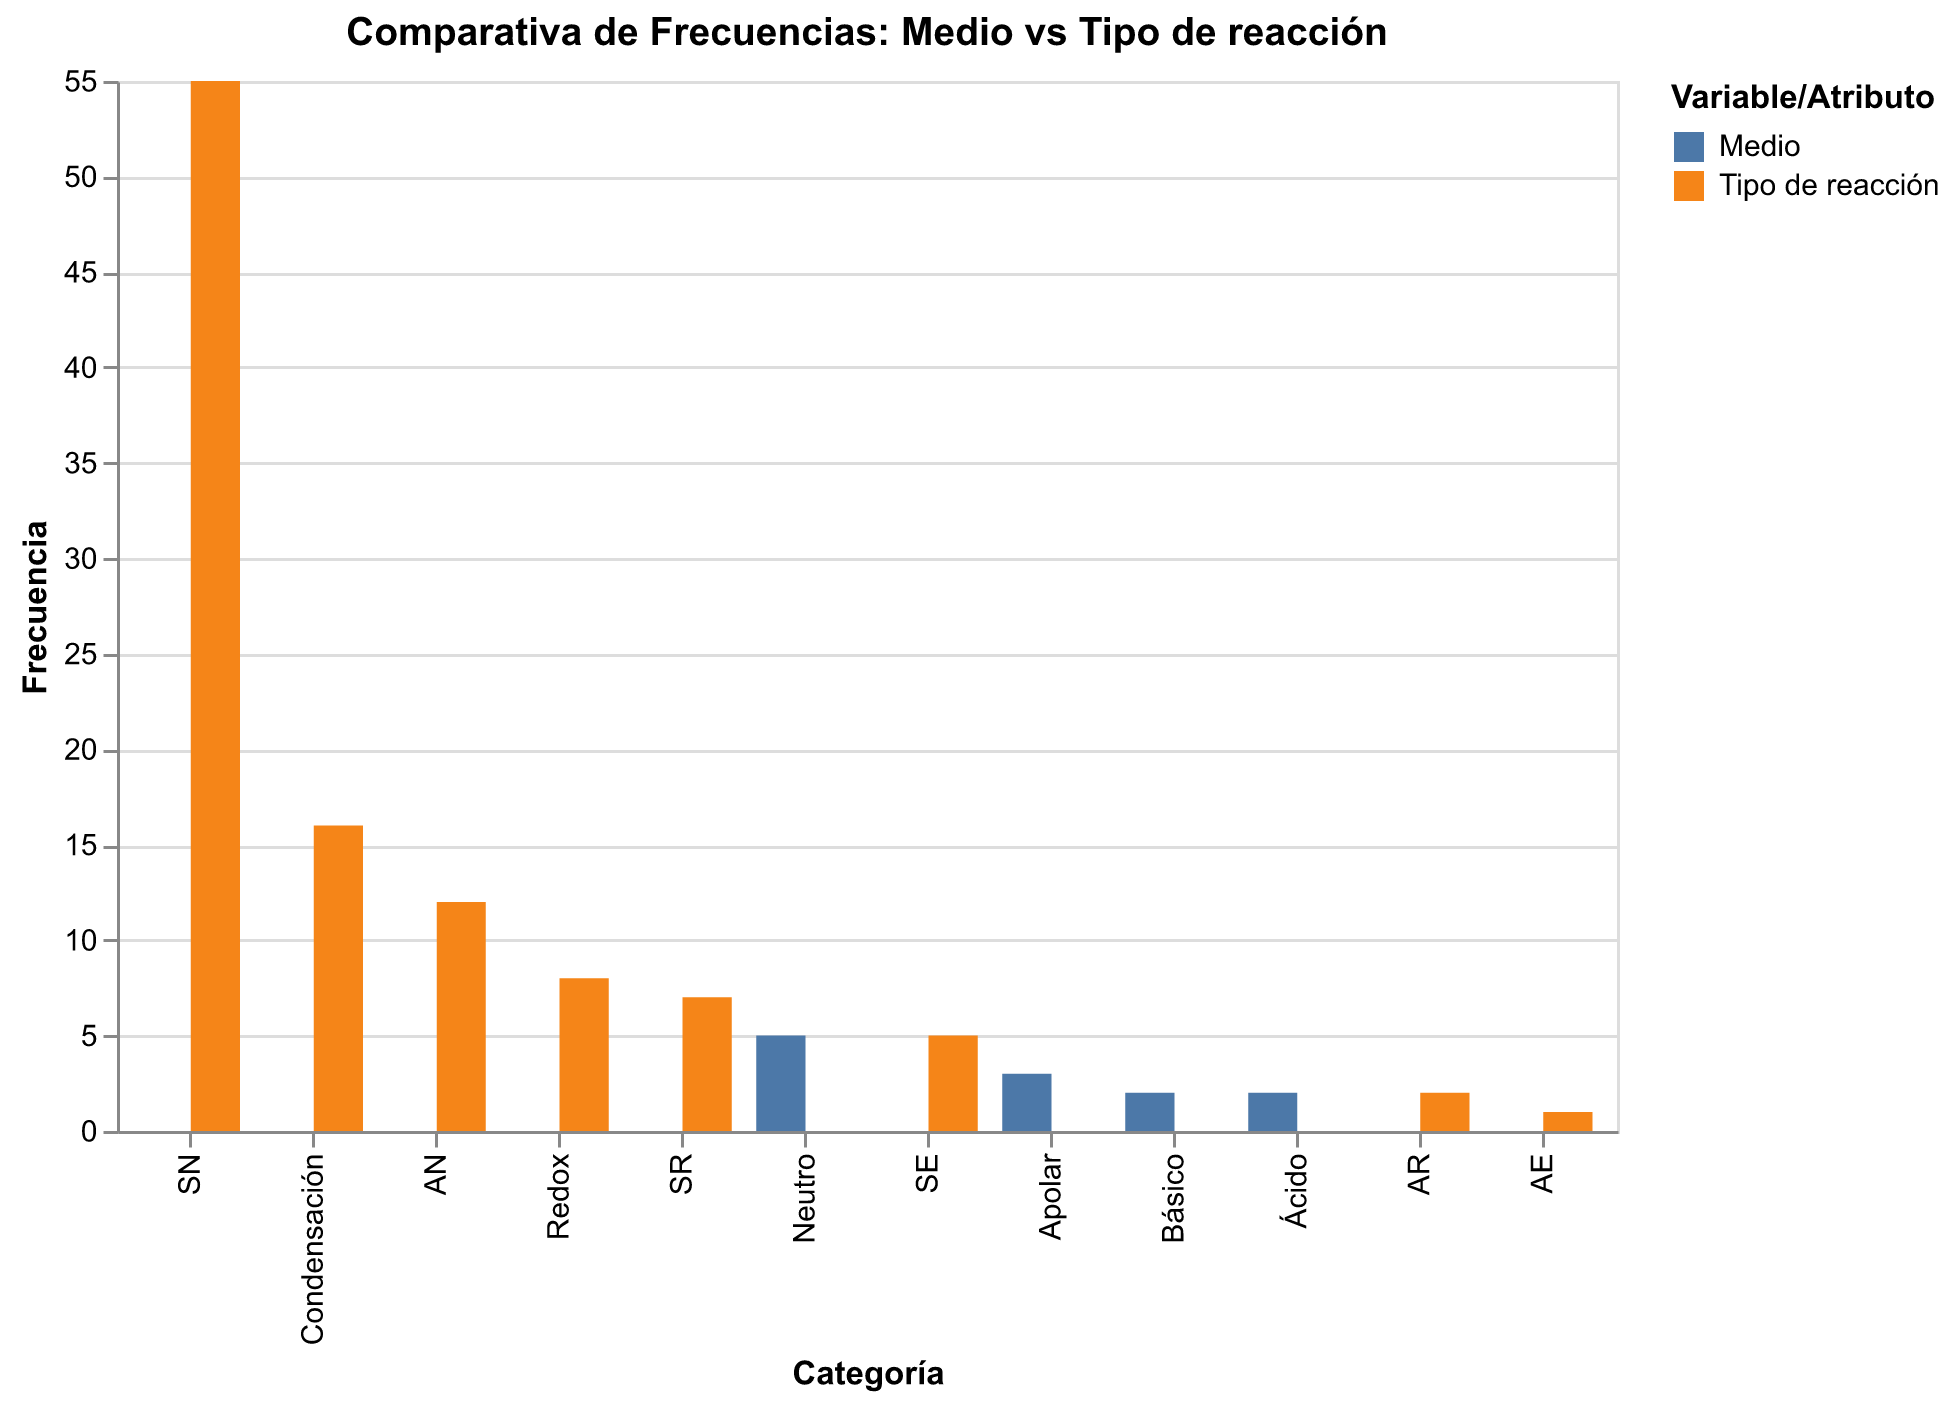
\includegraphics[width=\columnwidth]{09_frecuencias_medio_tipo.png}
	\caption{Frecuencia de los tipos de reacción y de los medios reportados.}
	\label{fig:frecuencias}
\end{figure}

\begin{figure}[htbp]
	\centering
	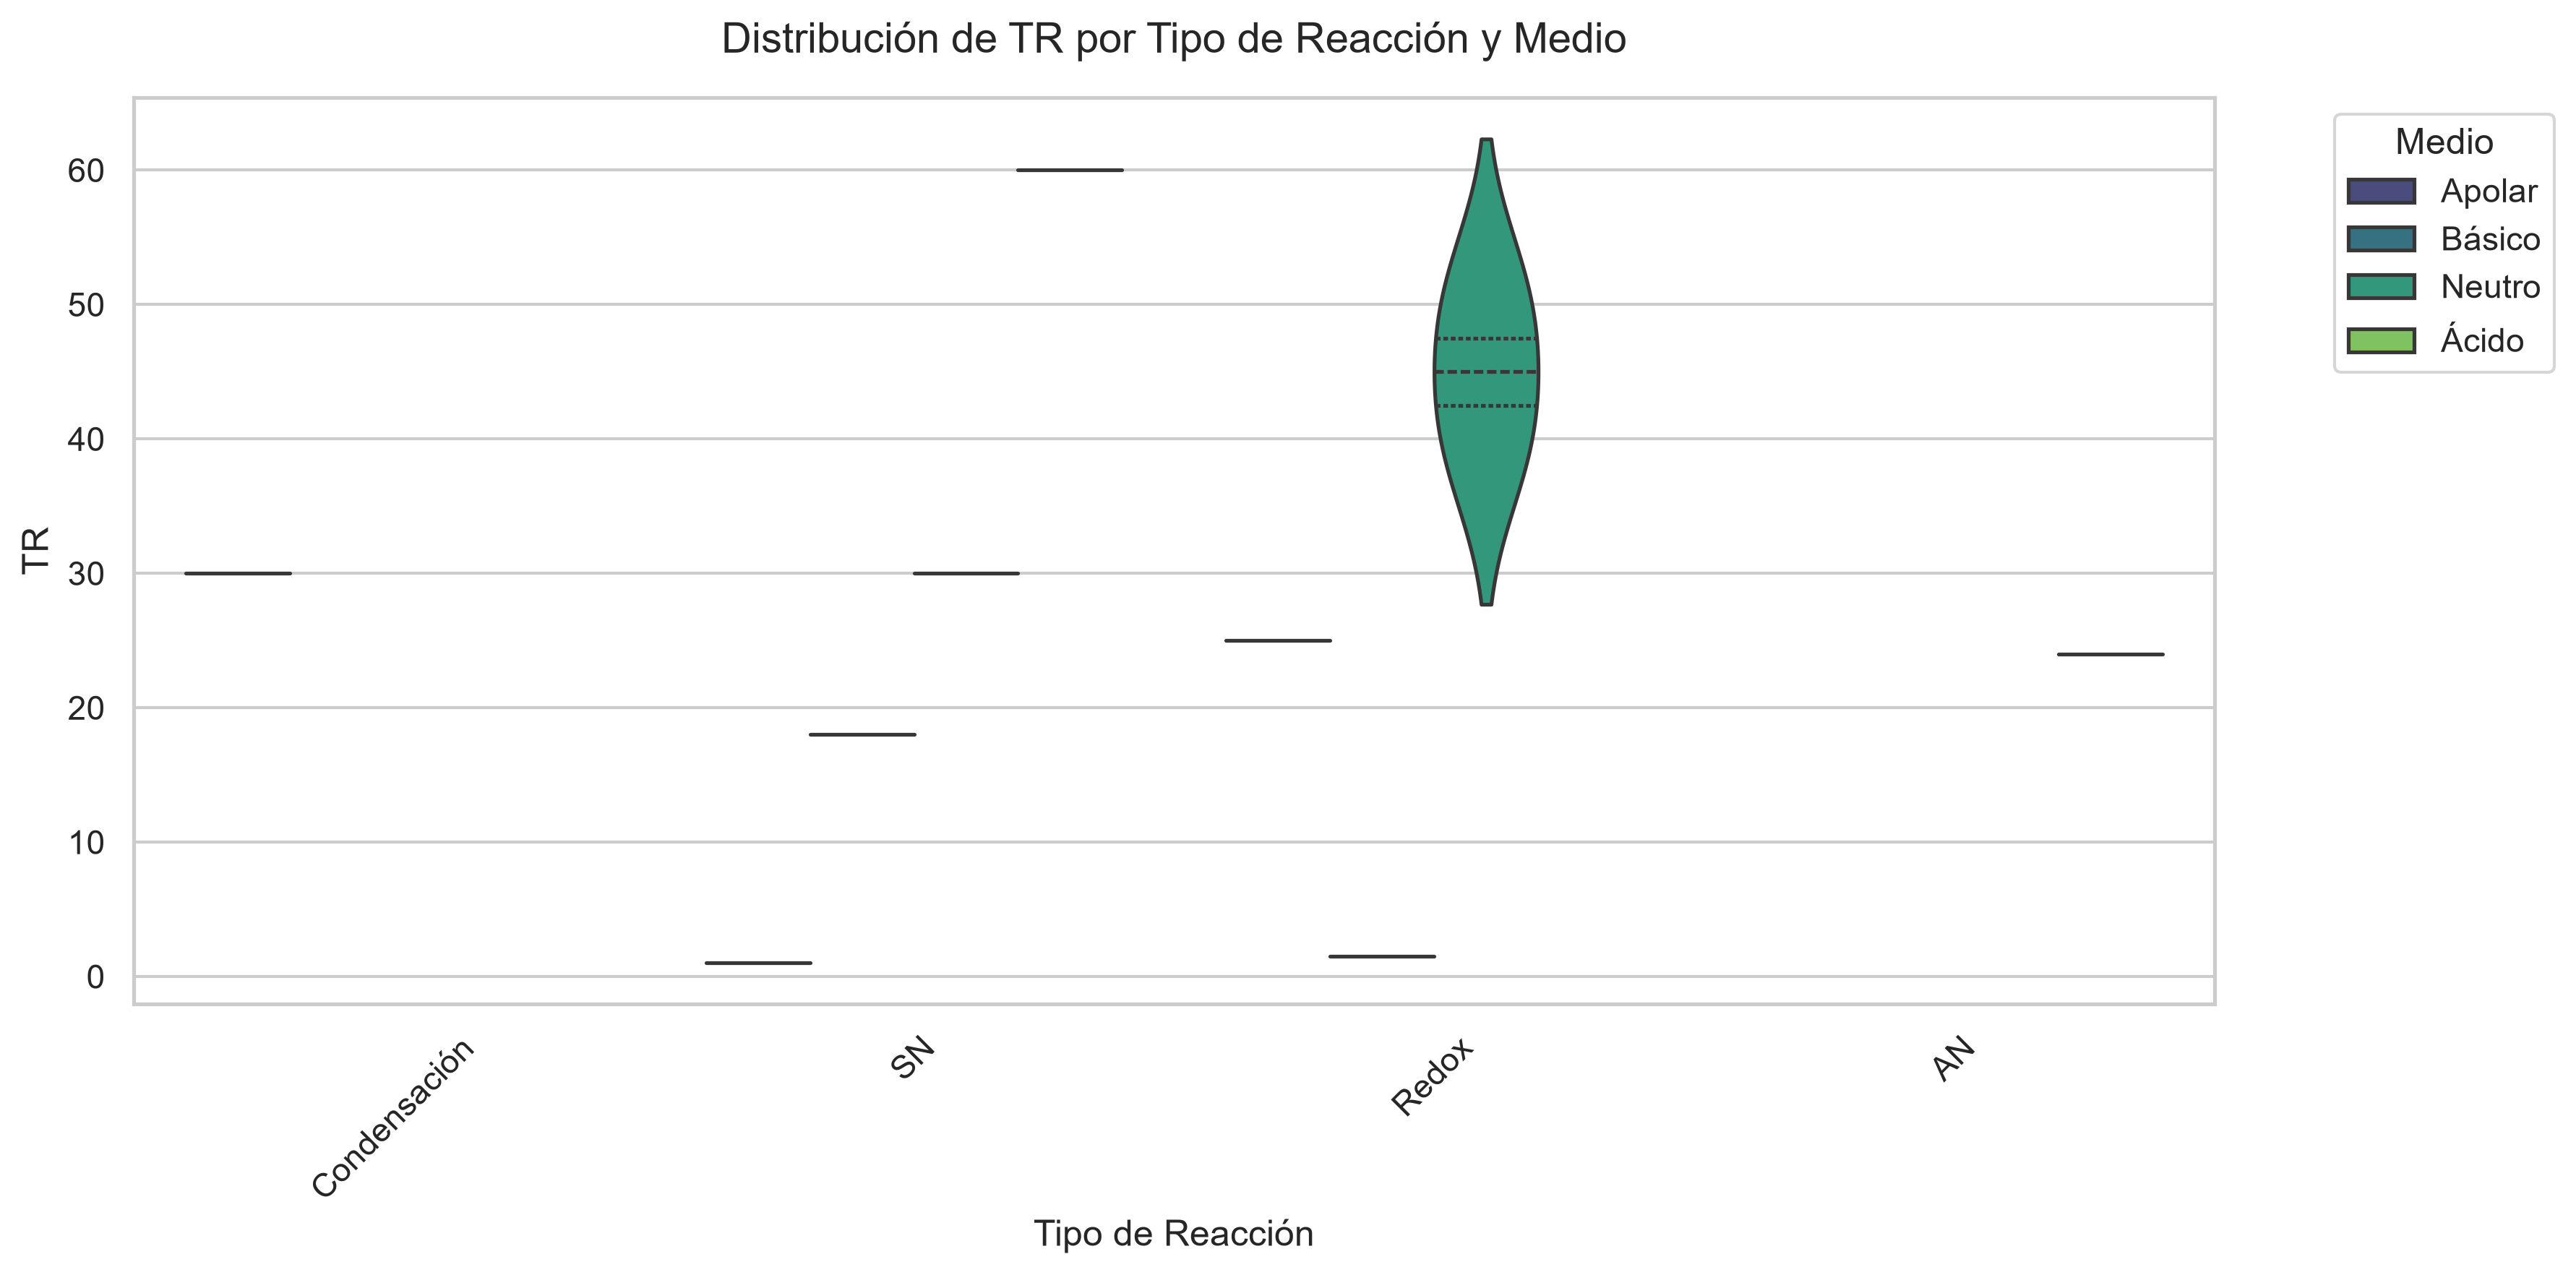
\includegraphics[width=\columnwidth]{07_violin_TR_tipo_medio.png}
	\caption{Distribución (violín) de TR por tipo de reacción y medio.}
	\label{fig:violin}
\end{figure}

\begin{figure}[htbp]
	\centering
	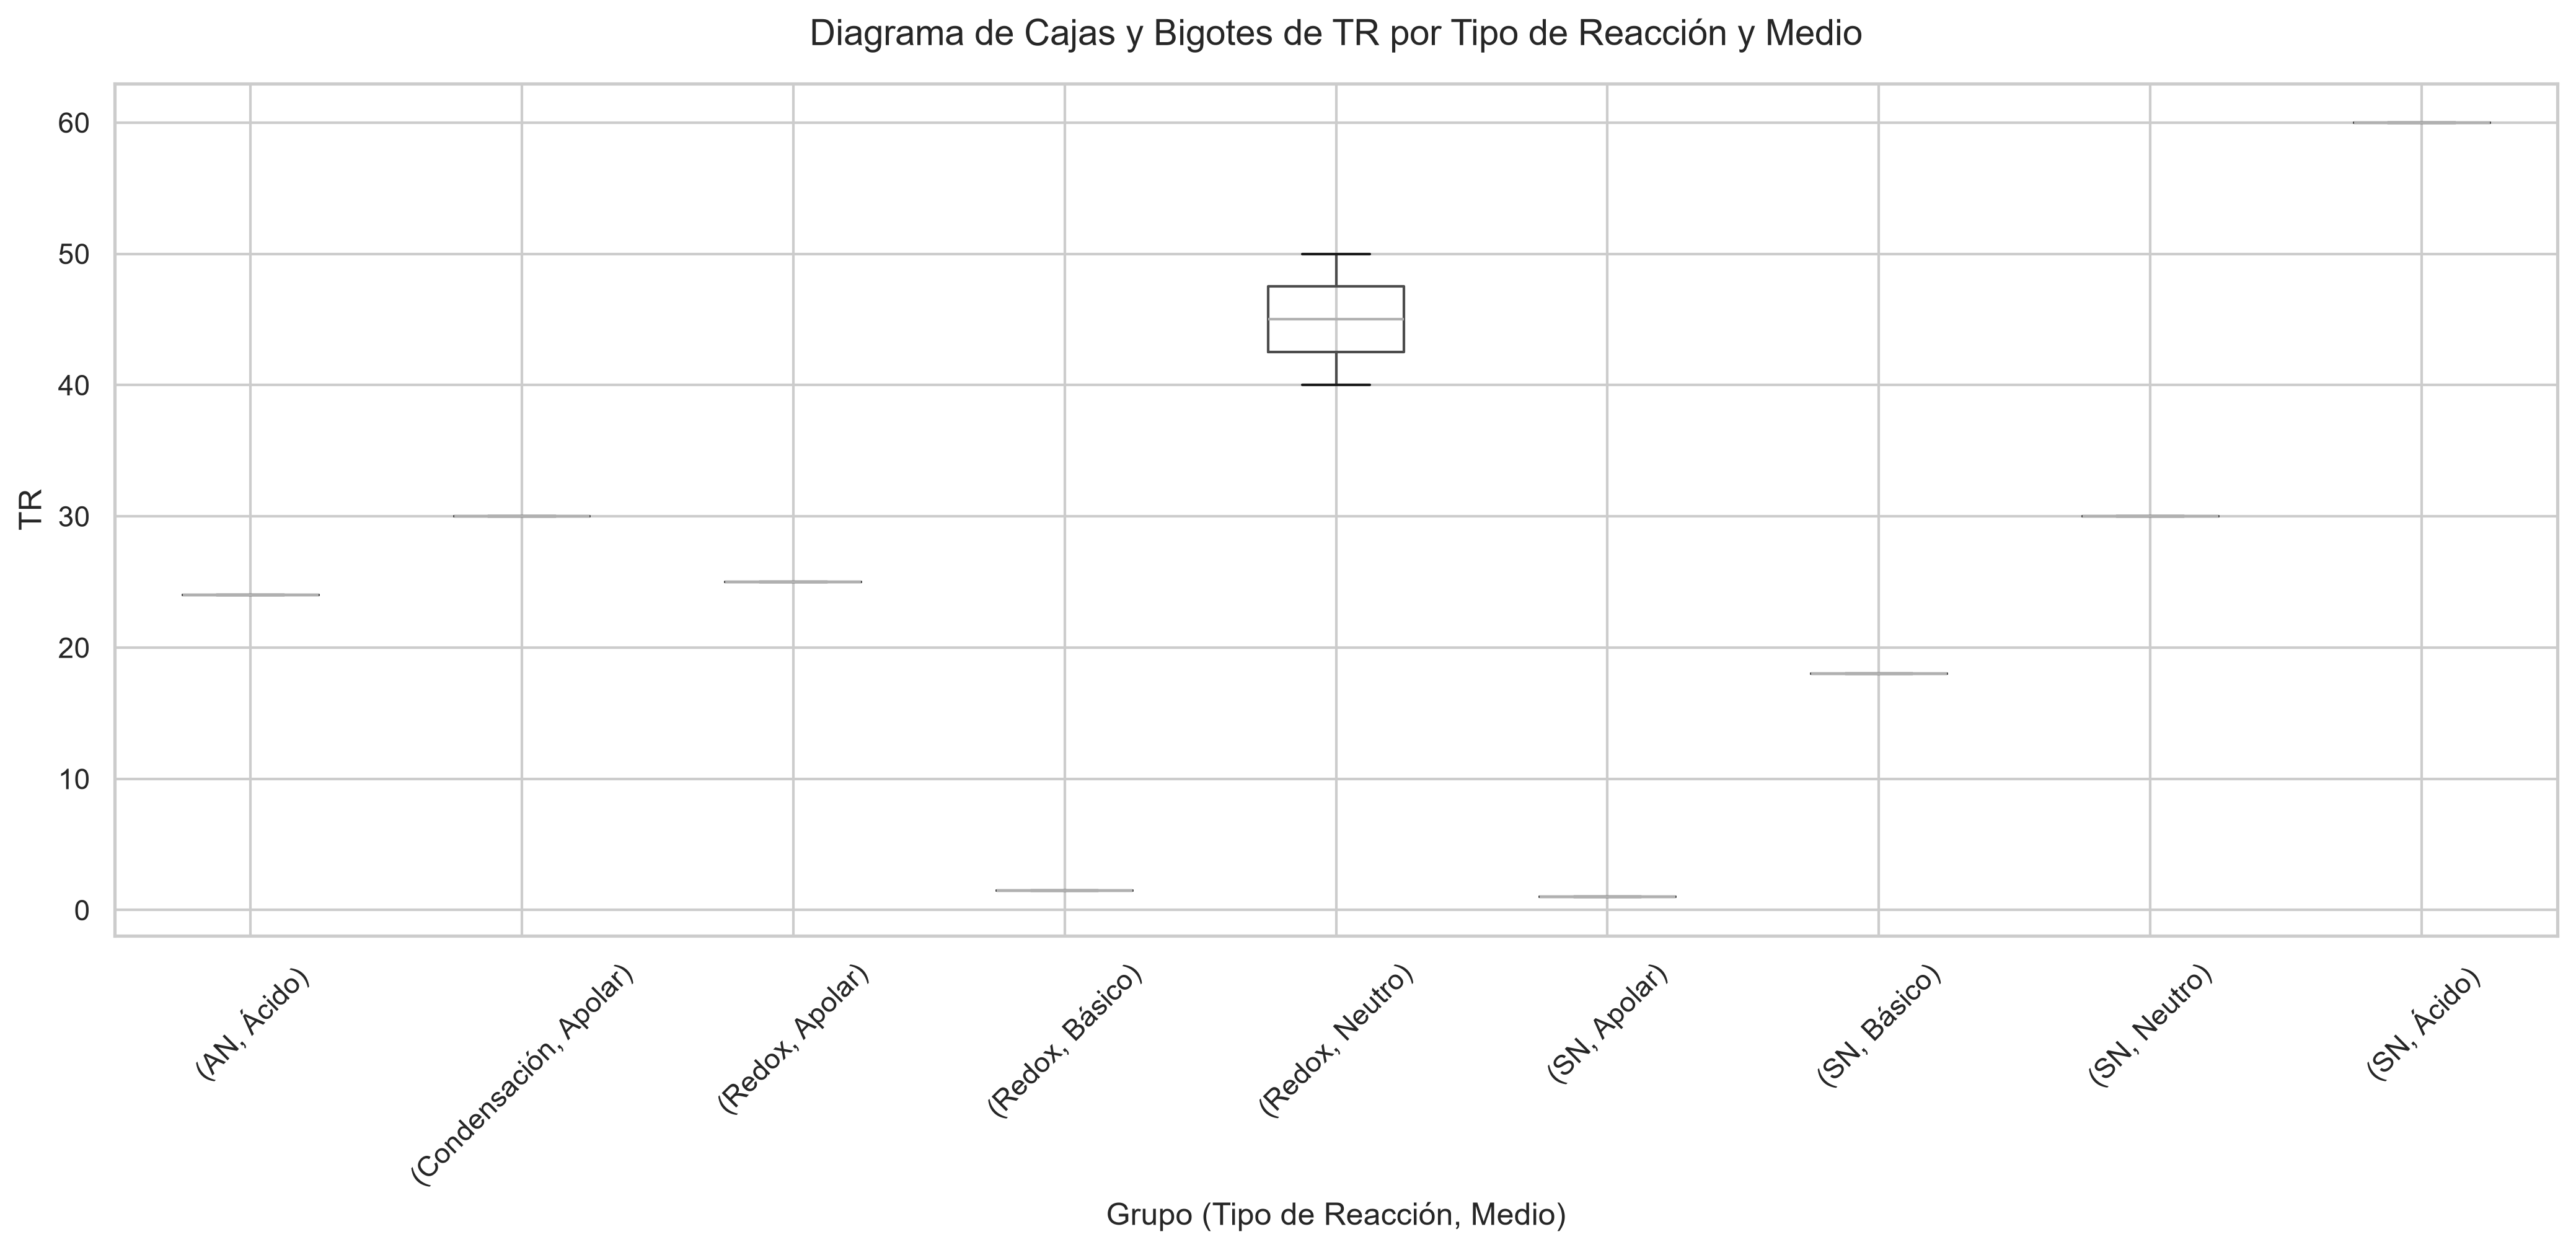
\includegraphics[width=\columnwidth]{08_boxplot_TR_tipo_medio.png}
	\caption{Diagrama de cajas y bigotes de TR por tipo de reacción y medio.}
	\label{fig:boxplot}
\end{figure}

\begin{figure}[htbp]
	\centering
	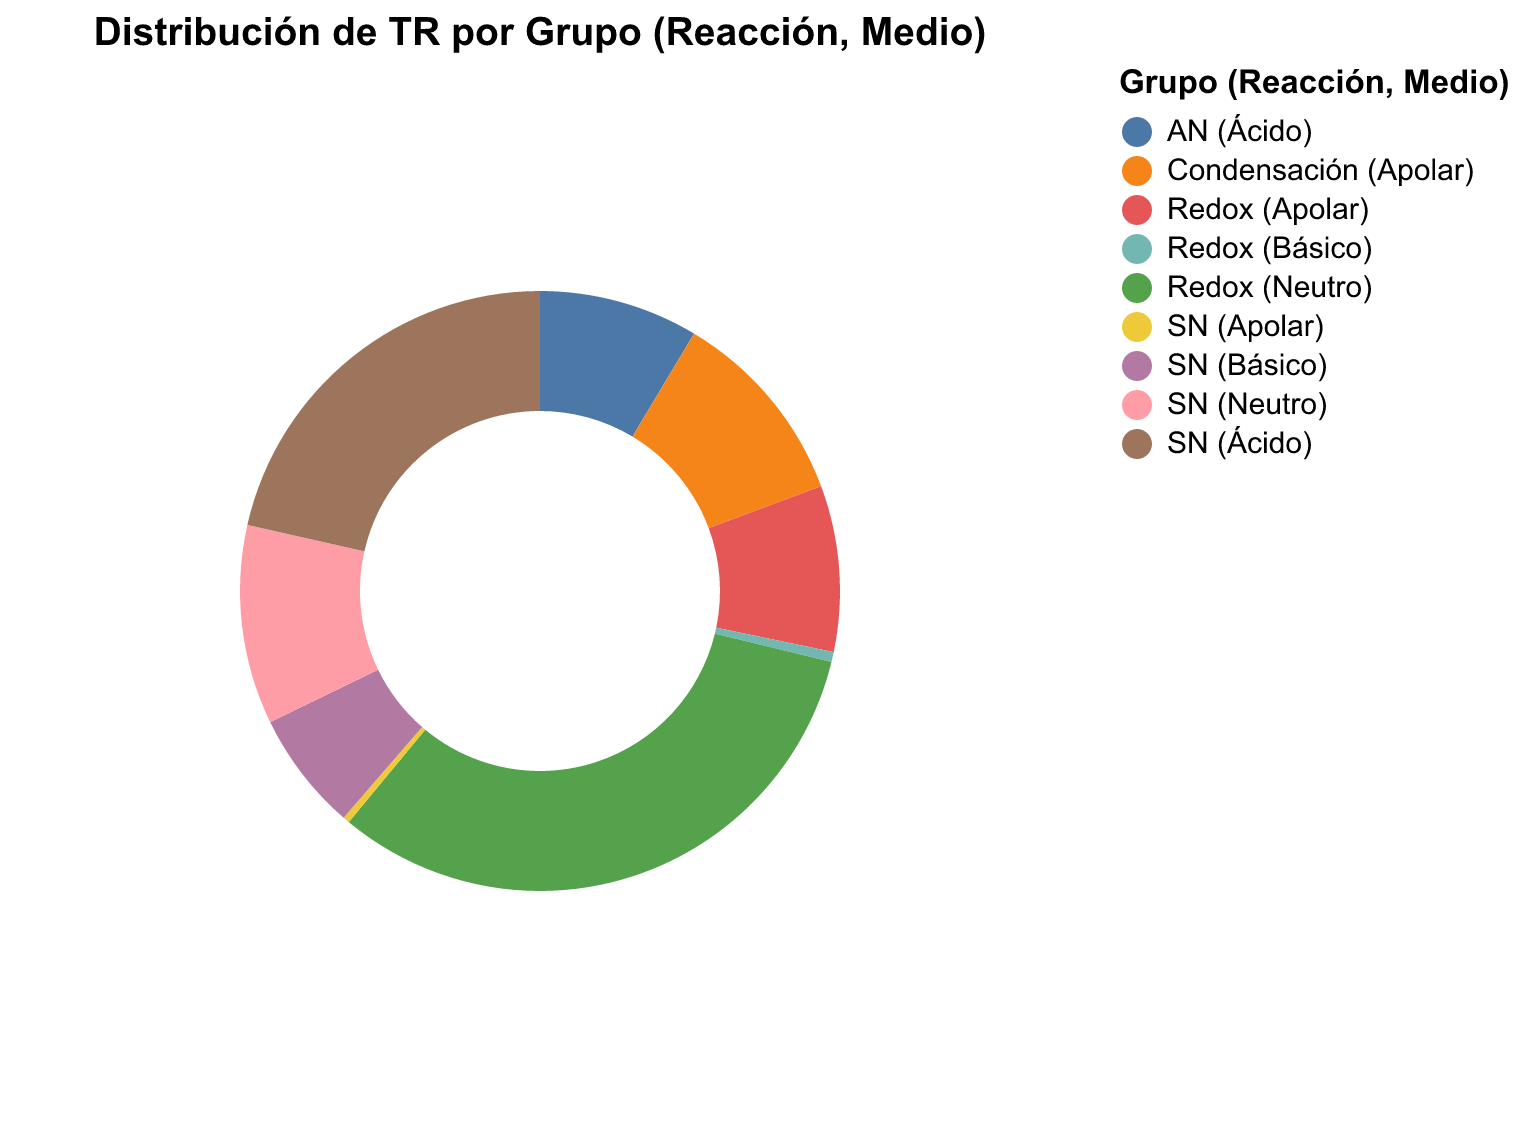
\includegraphics[width=0.9\columnwidth]{10_dona_TR_grupo.png}
	\caption{Participación de TR por grupo (tipo de reacción, medio).}
	\label{fig:dona}
\end{figure}

\section{Conclusiones y Perspectiva}
\fontsize{12}{14}\selectfont
% TODO (Valentina): 3--5 conclusiones que respondan al objetivo de la introducción,
% cada una sustentada en una figura o en la Tabla~\ref{tab:propiedades}.
\textit{[Redacción pendiente.]}

%  Contenido: Metodología, Análisis Gráfico (Colab/Conda) y Conclusiones
%
%  Reglas para editar sin romper la compilación:
%   * NO escribir \documentclass, \begin{document} ni \end{document} aquí.
%   * Las figuras están en ../imagenes/ y se llaman sólo por su nombre
%     (main.tex ya define \graphicspath{{imagenes/}}).
%   * Referenciar figuras con Figura~\ref{fig:...}, nunca "la figura de abajo".
% =====================================================================

\section{Metodología}
\fontsize{12}{14}\selectfont
% TODO (Valentina): pegar aquí la redacción de la metodología.

\subsection{Recolección de datos}
\textit{[Redacción pendiente: búsqueda en CAS-SciFinder, compuestos e indicadores asignados, consolidación en Excel con formato Tabla.]}

\subsection{Limpieza y procesamiento en Python}
\textit{[Redacción pendiente: Google Colab con Pandas, NumPy, Matplotlib, Seaborn y Plotly; filtrado de los compuestos de interés, conversión de comas decimales, tratamiento de valores nulos y atípicos.]}

\subsection{Análisis estadístico}
\textit{[Redacción pendiente: correlación de Spearman (no paramétrica, robusta a valores atípicos y relaciones monótonas no lineales), regresiones lineales con intervalo de confianza del 95\,\% y distribuciones por tipo de reacción y medio.]}

\section{Resultados y Discusión}
\fontsize{12}{14}\selectfont

\subsection{Correlación entre propiedades}
% TODO (Valentina): interpretar los coeficientes más fuertes (positivos y negativos).
La Figura~\ref{fig:heatmap} presenta la matriz de correlación de Spearman entre
las propiedades fisicoquímicas, y la Figura~\ref{fig:clustermap} agrupa
jerárquicamente las variables con comportamiento similar.
\textit{[Interpretación pendiente.]}

\begin{figure}[htbp]
	\centering
	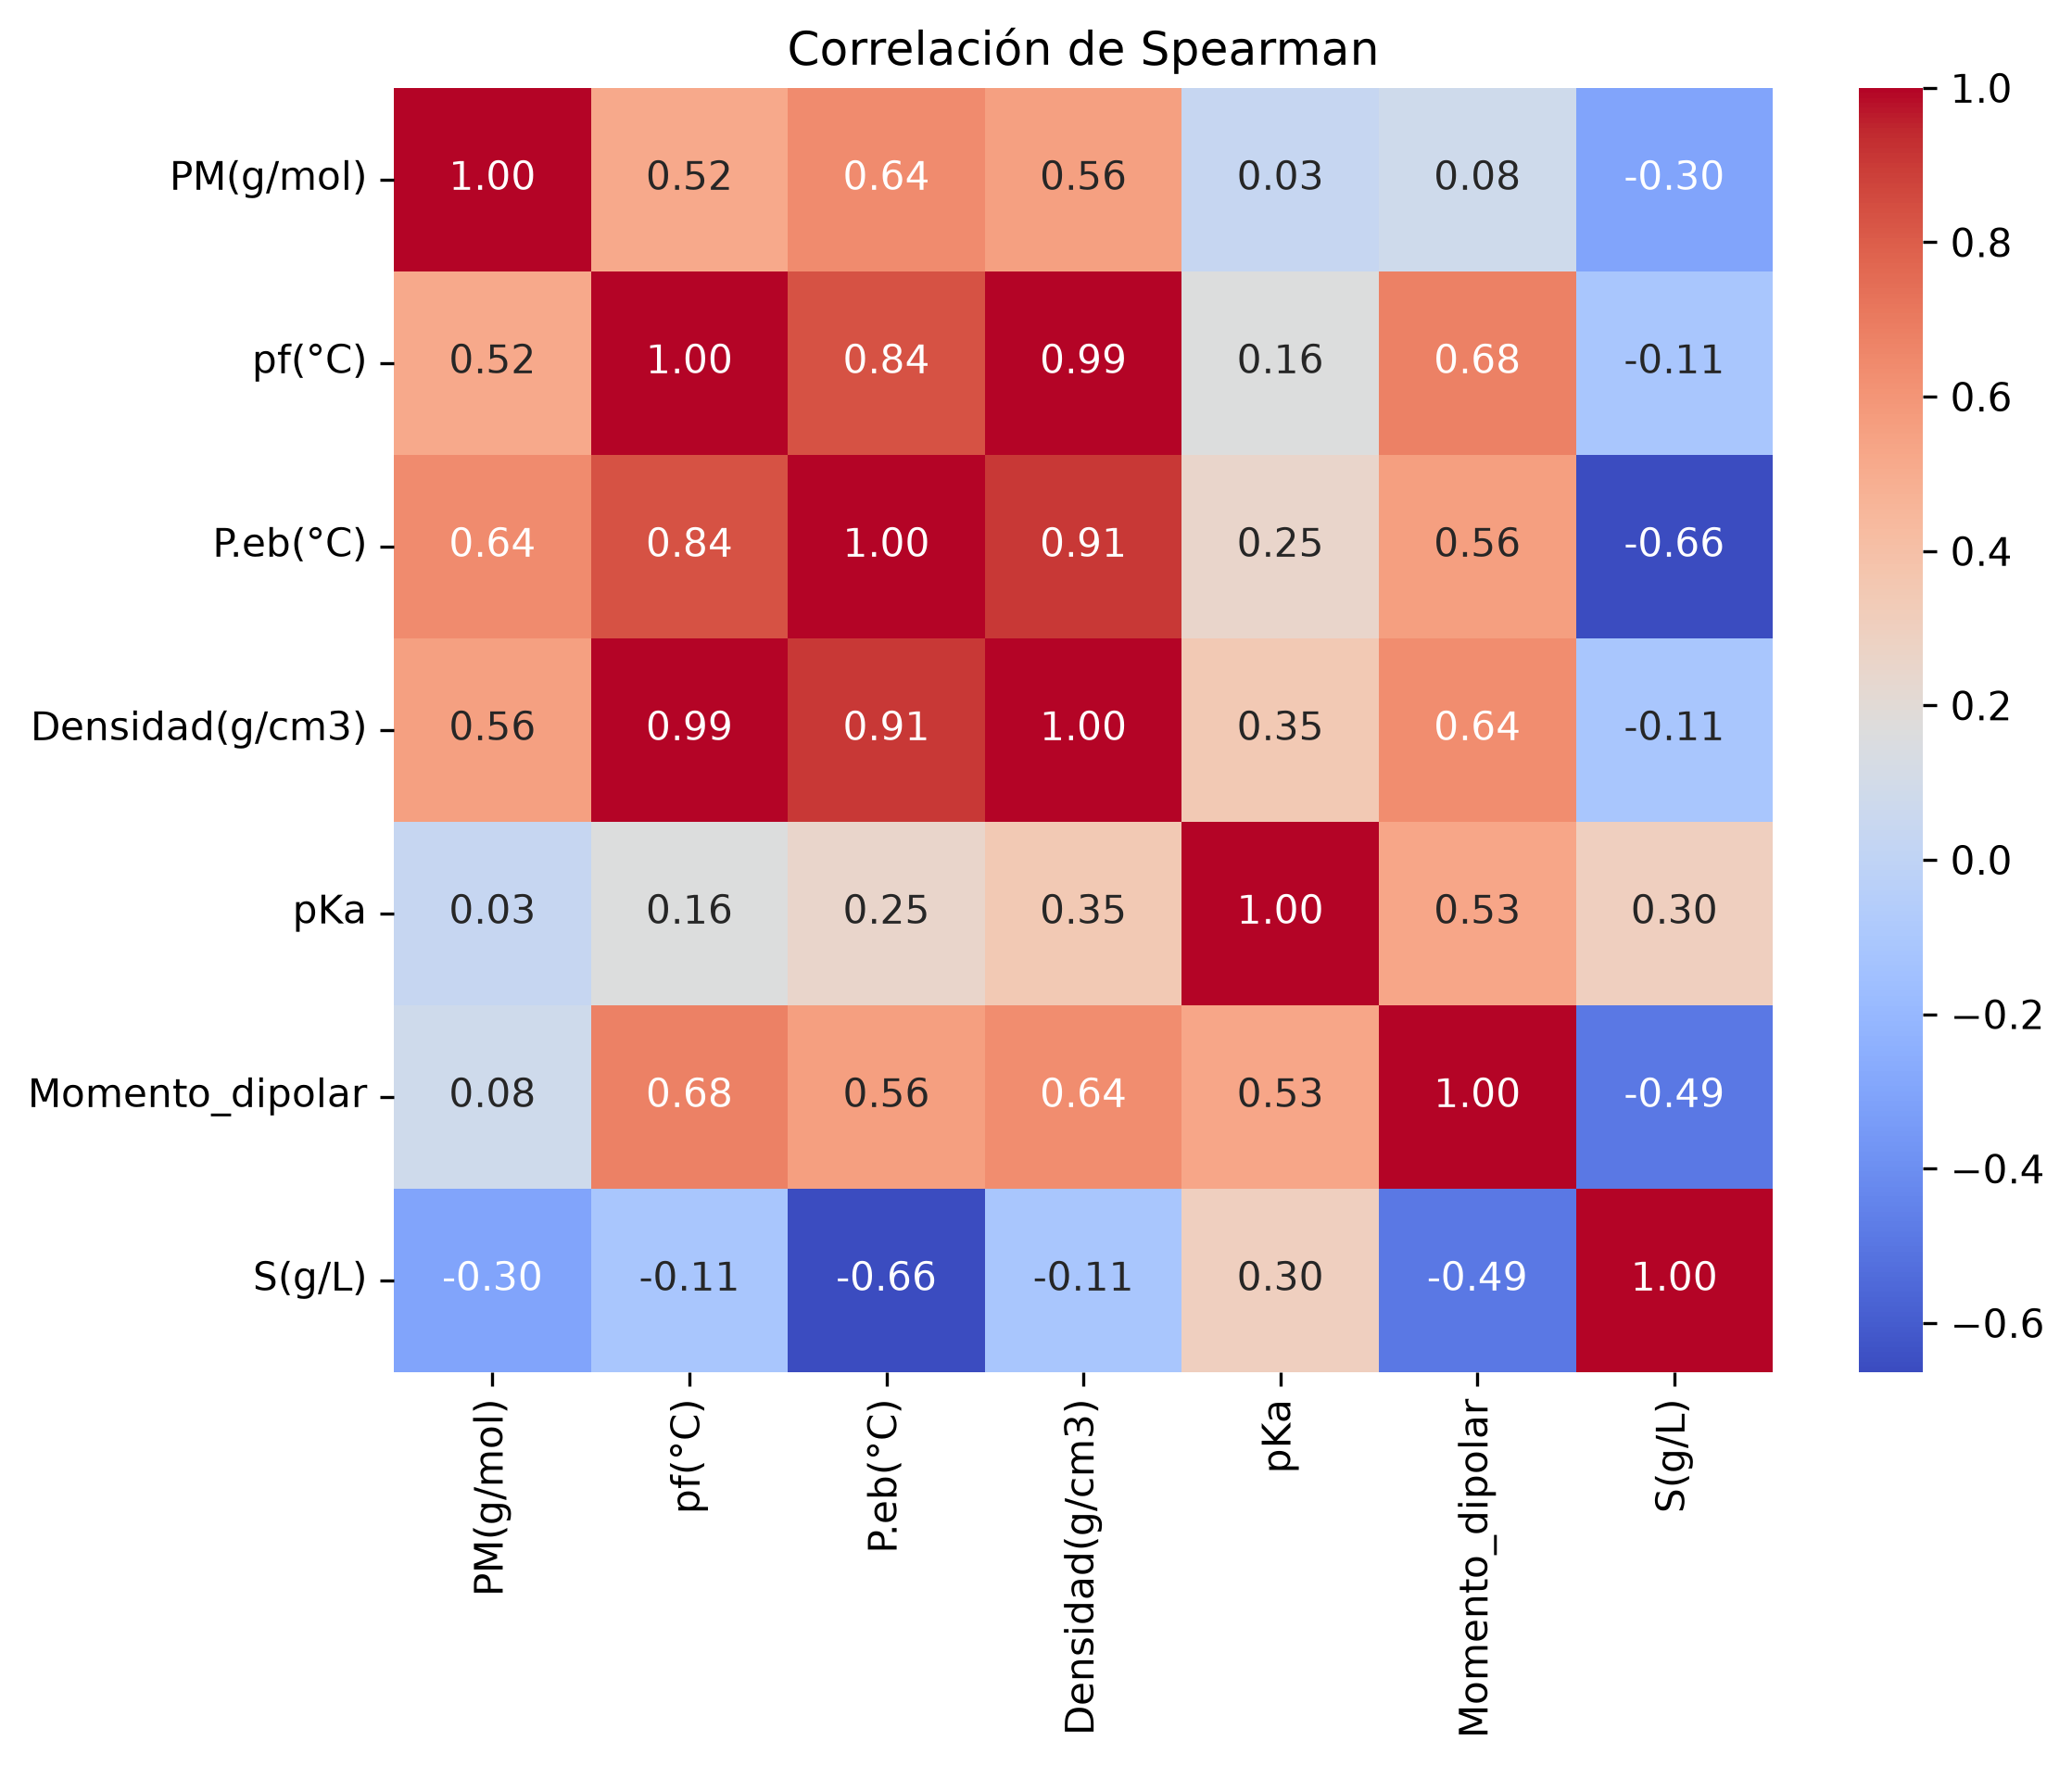
\includegraphics[width=\columnwidth]{01_heatmap_spearman.png}
	\caption{Matriz de correlación de Spearman entre las propiedades fisicoquímicas.}
	\label{fig:heatmap}
\end{figure}

\begin{figure}[htbp]
	\centering
	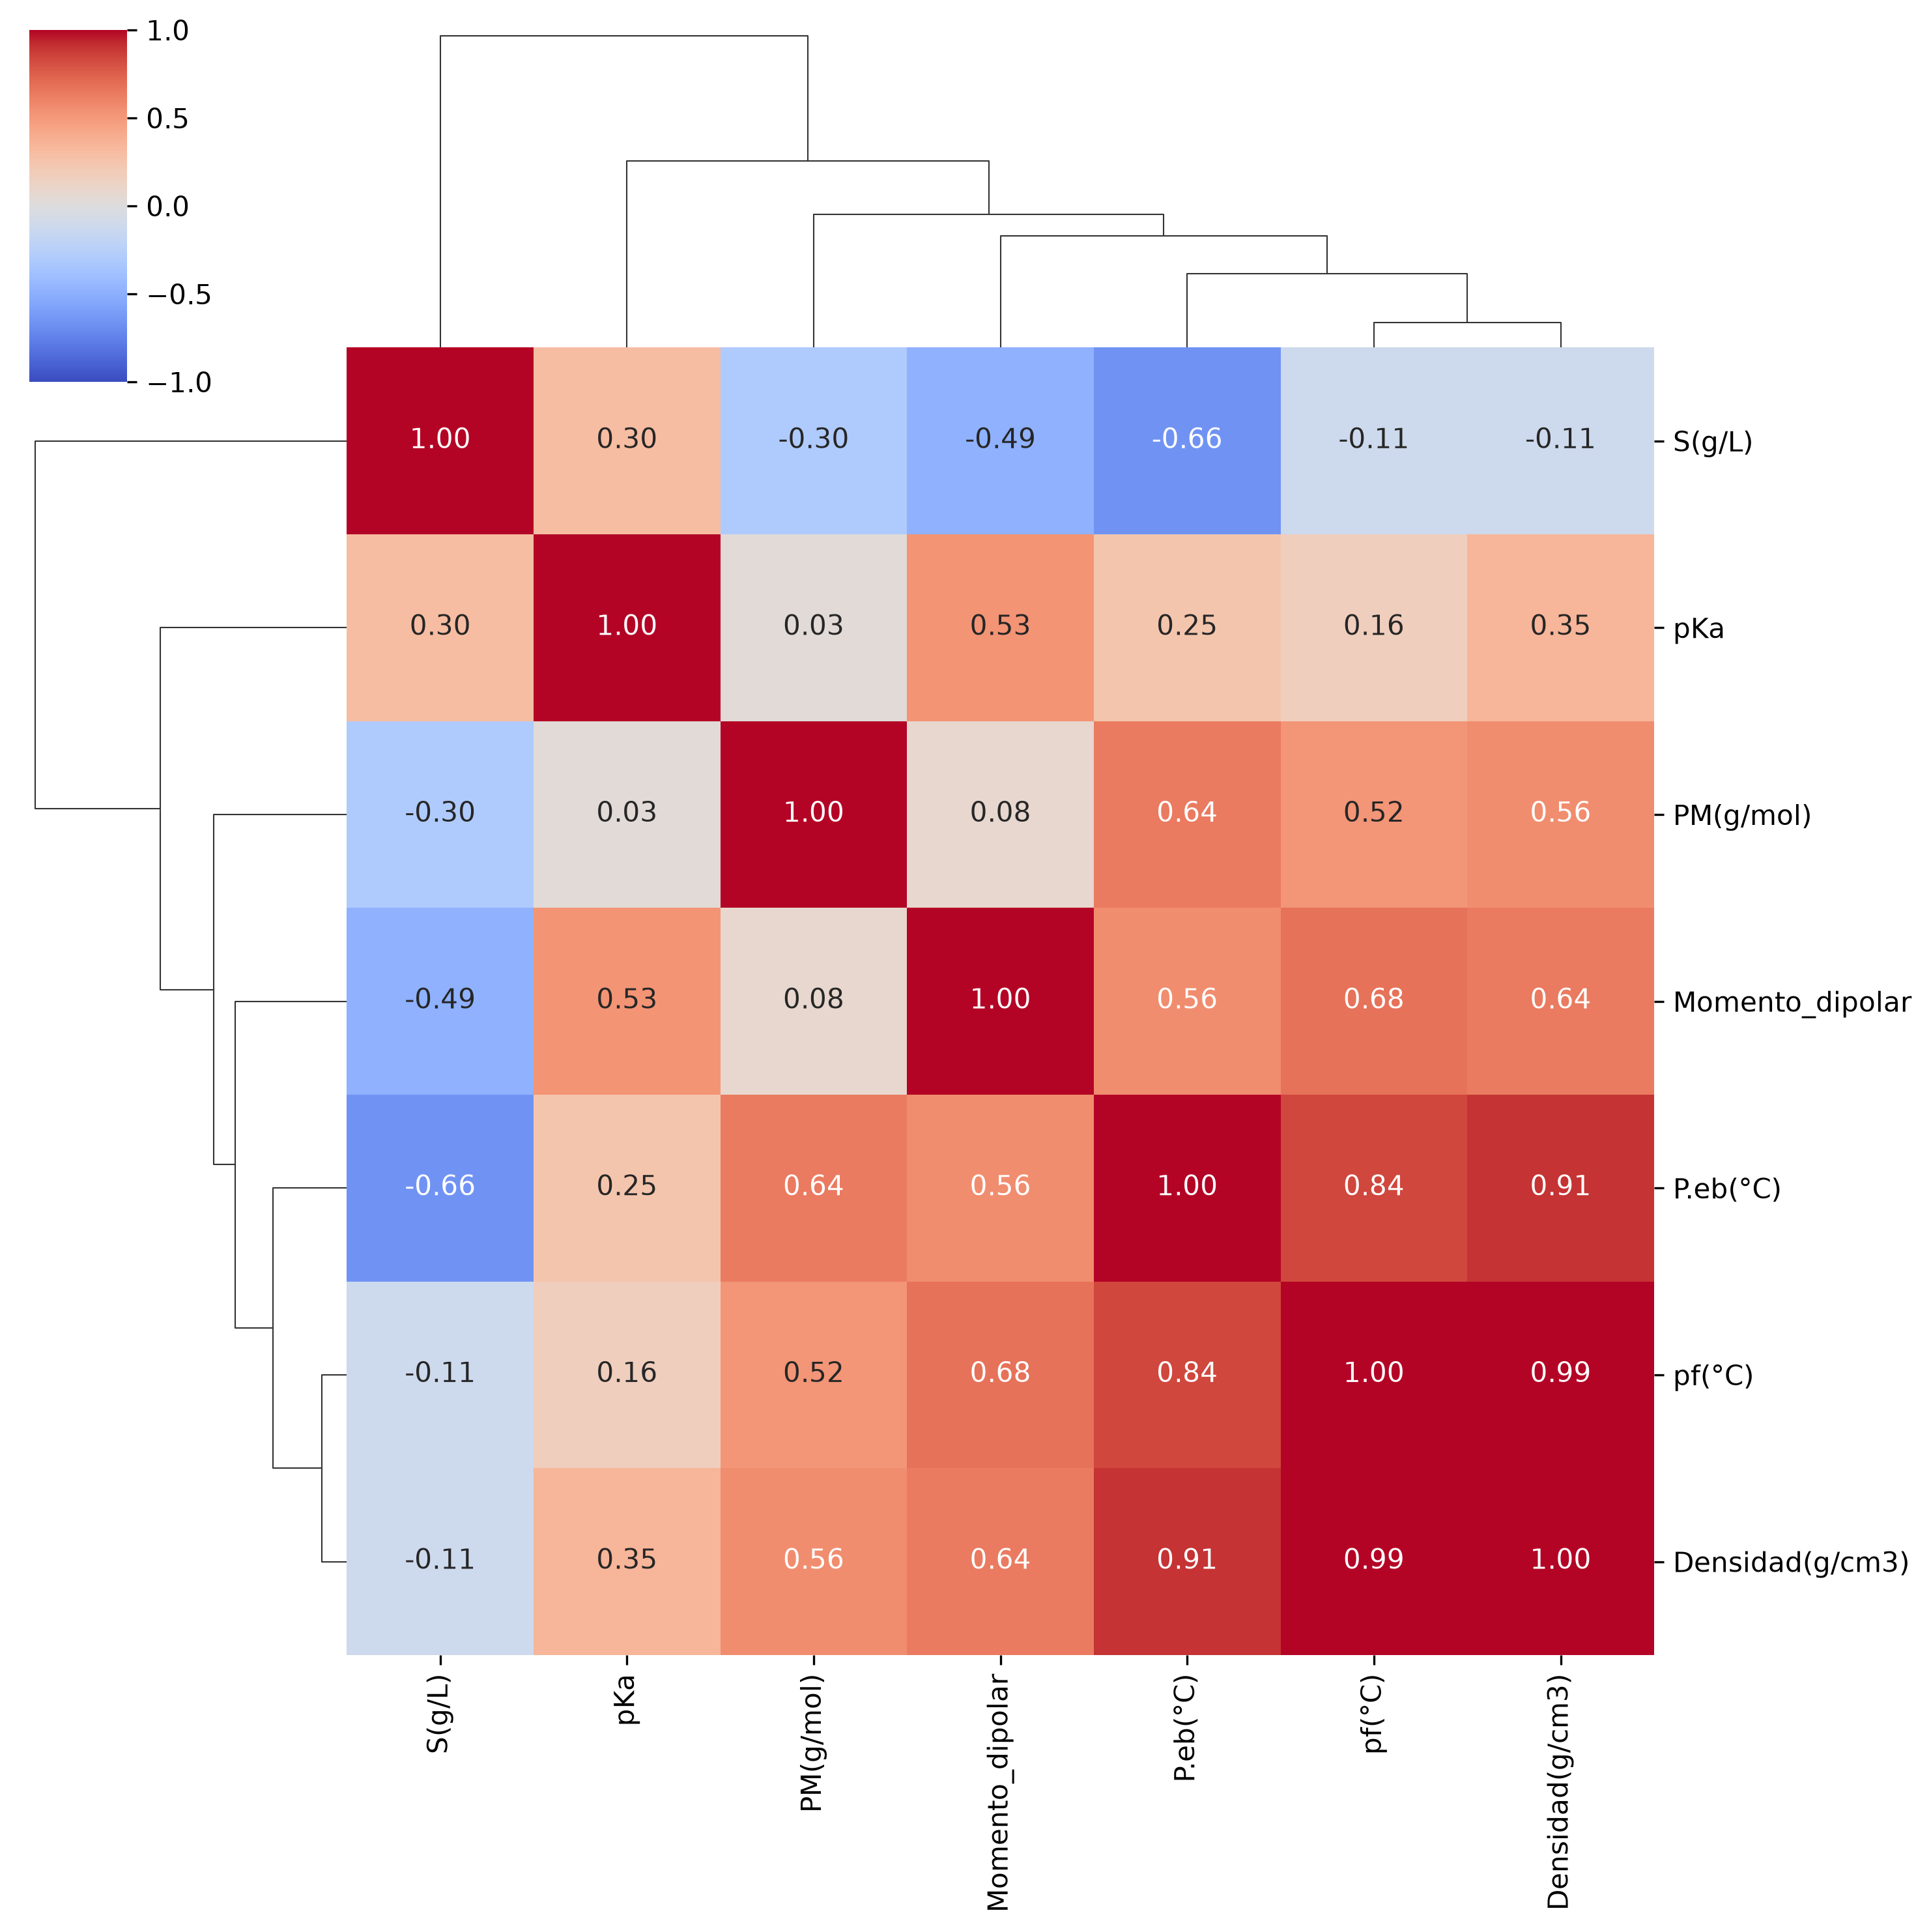
\includegraphics[width=\columnwidth]{02_clustermap_spearman.png}
	\caption{Mapa de agrupamiento jerárquico de la correlación de Spearman.}
	\label{fig:clustermap}
\end{figure}

\subsection{Tendencias entre propiedades}
% TODO (Valentina): discutir cada regresión en términos de fuerzas intermoleculares.
Las Figuras~\ref{fig:pf-dens}--\ref{fig:dip-peb} muestran las regresiones
lineales entre pares de propiedades, con su intervalo de confianza.
\textit{[Interpretación pendiente.]}

\begin{figure}[htbp]
	\centering
	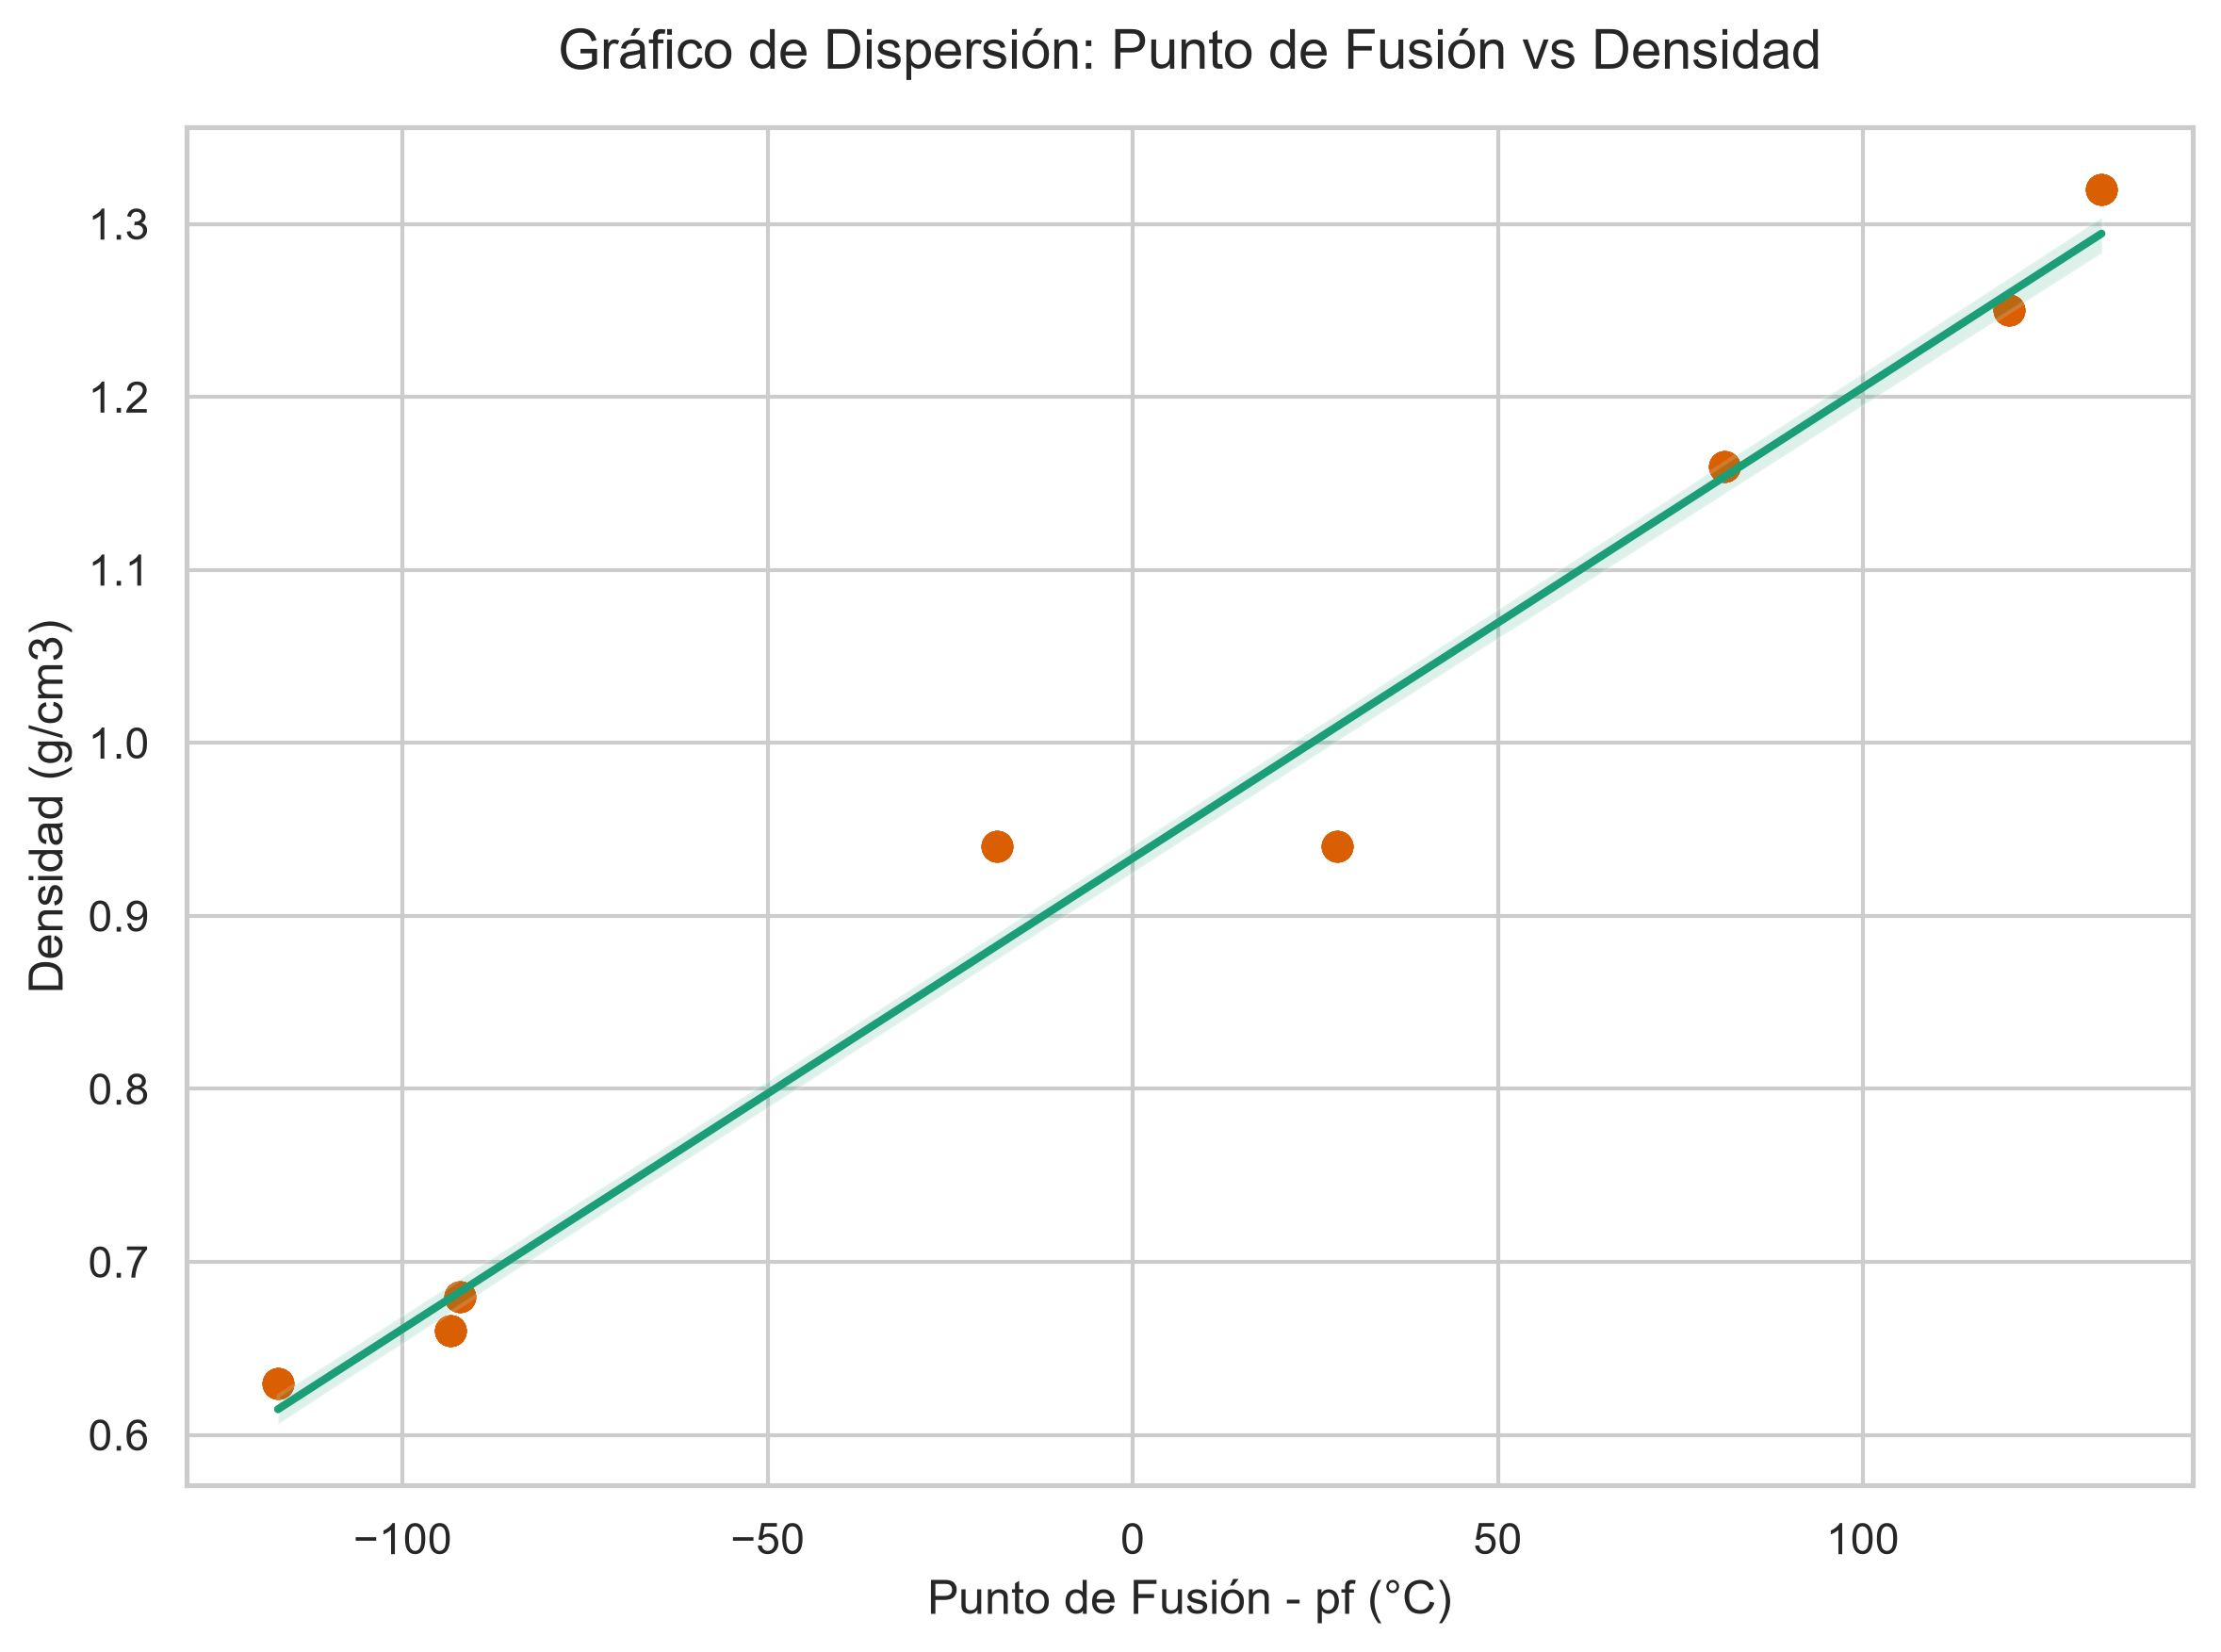
\includegraphics[width=\columnwidth]{03_reg_pf_vs_densidad.png}
	\caption{Punto de fusión frente a densidad.}
	\label{fig:pf-dens}
\end{figure}

\begin{figure}[htbp]
	\centering
	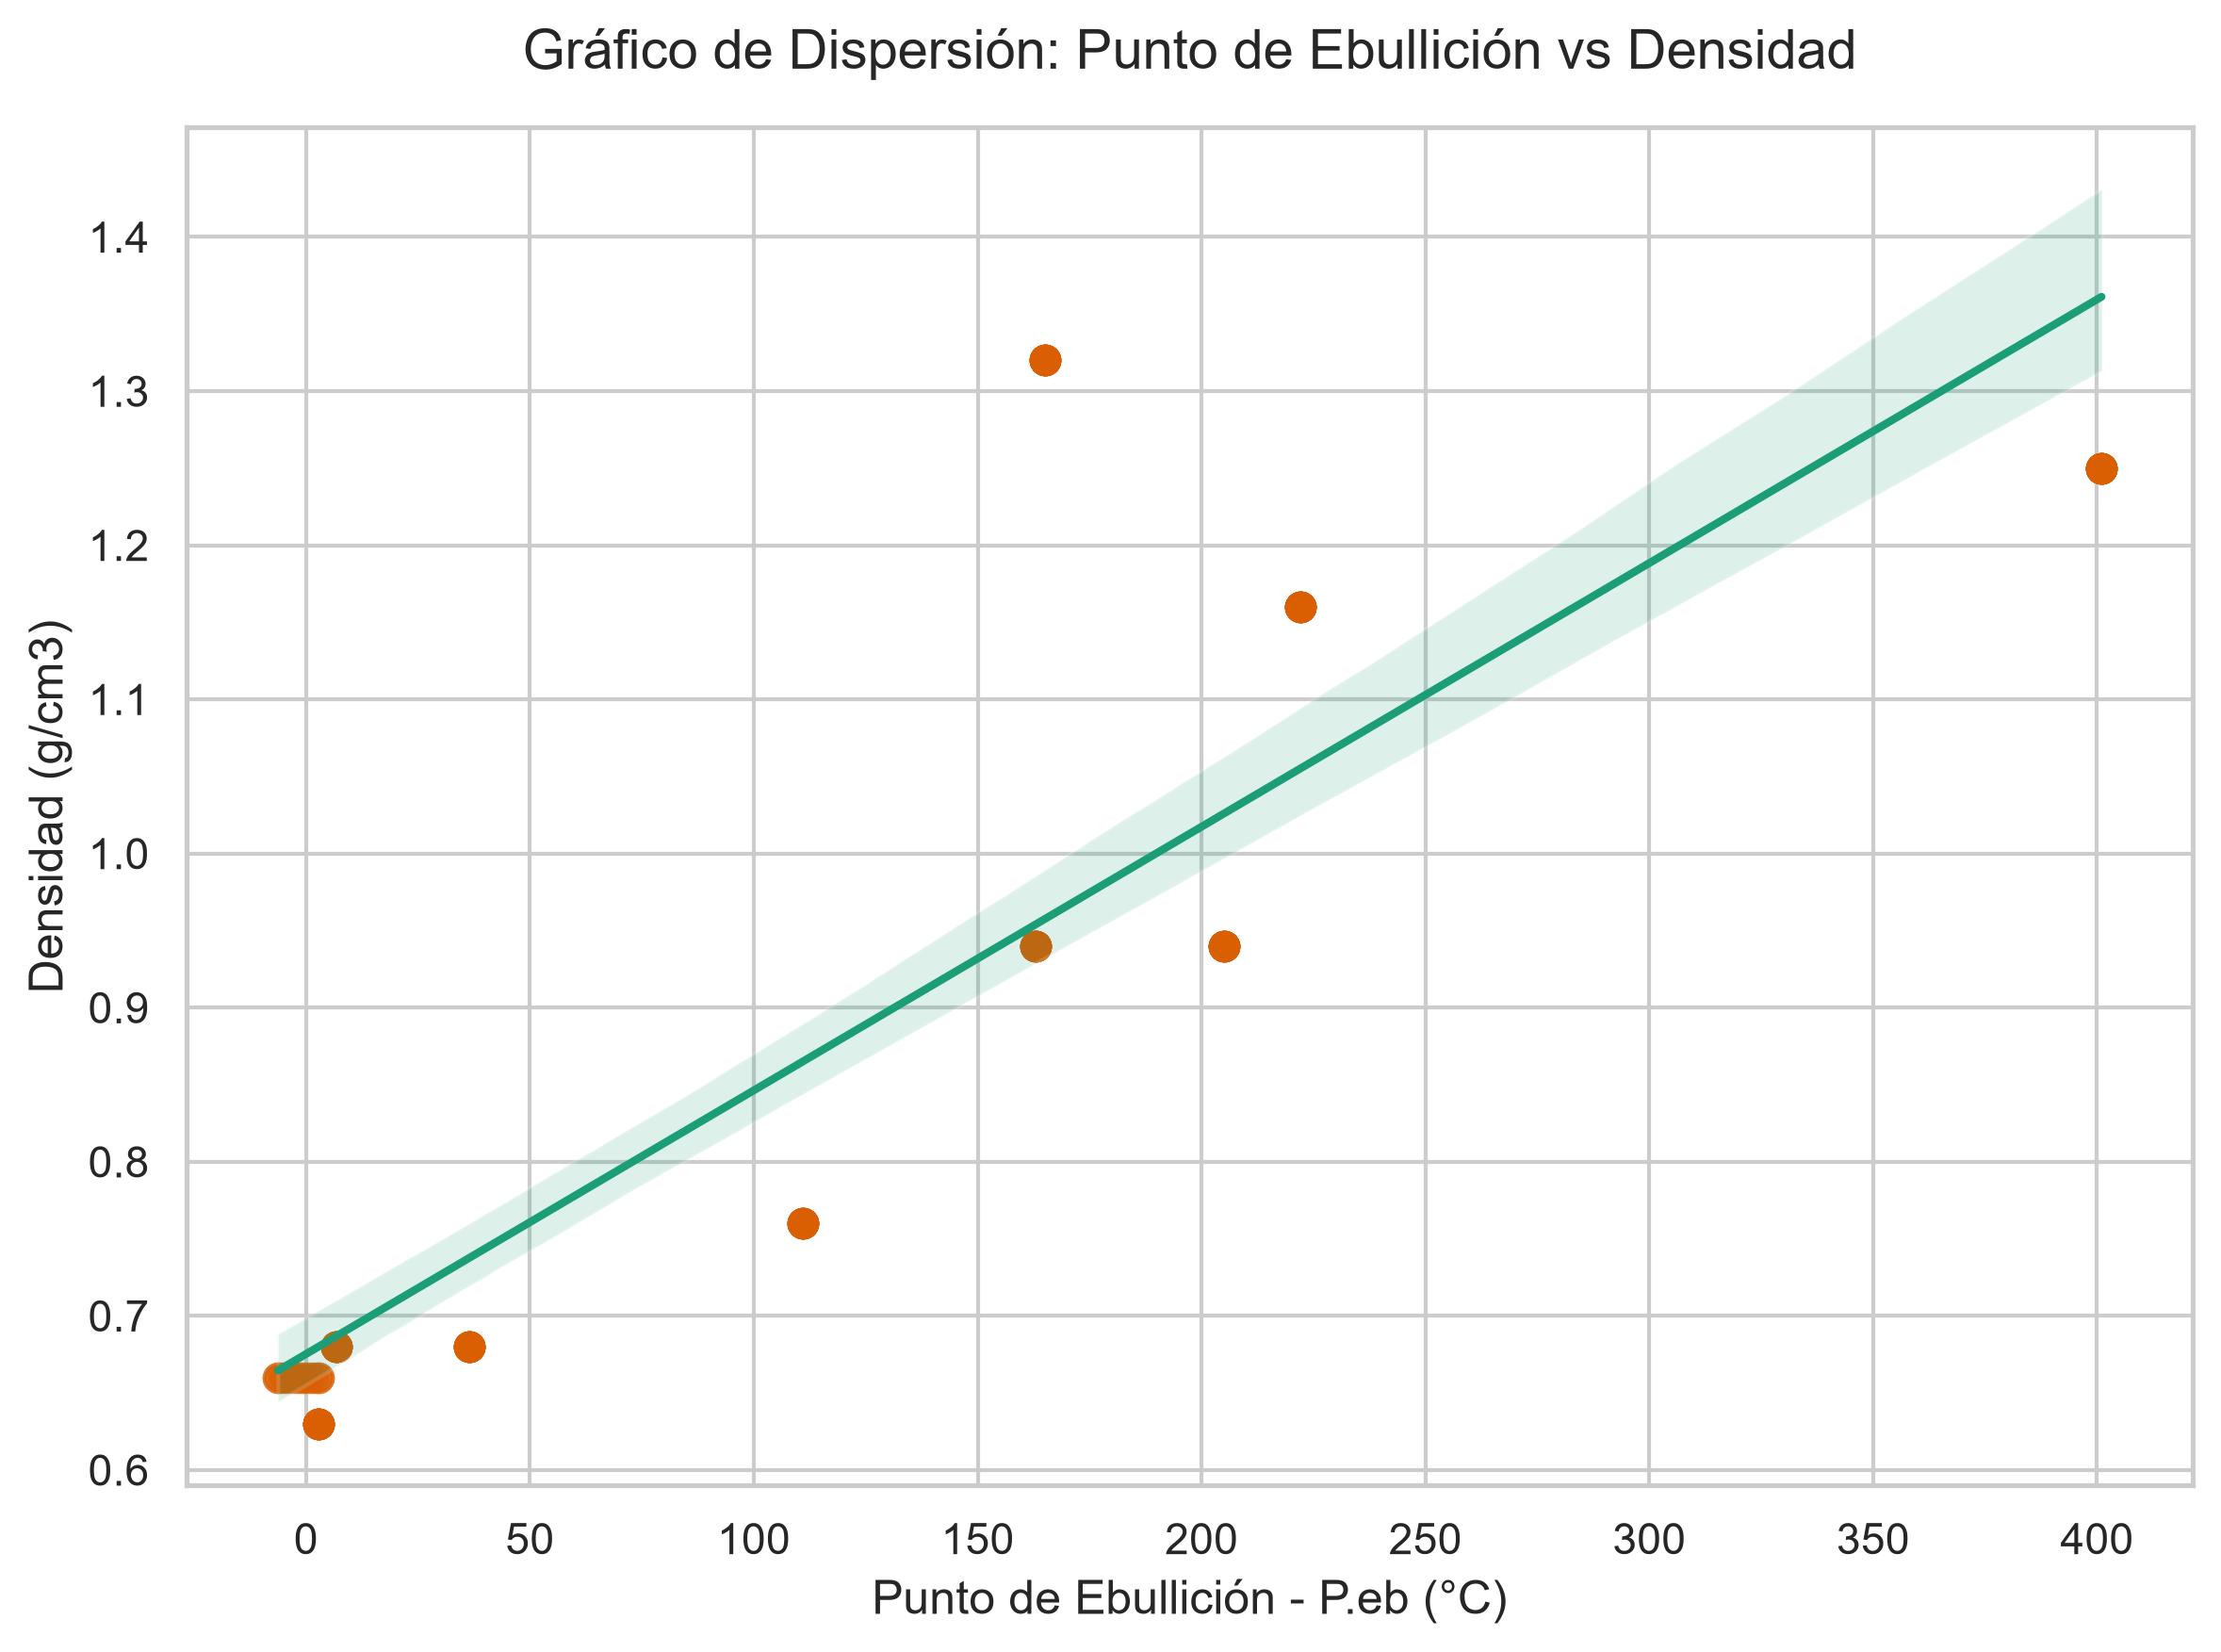
\includegraphics[width=\columnwidth]{04_reg_peb_vs_densidad.png}
	\caption{Punto de ebullición frente a densidad.}
	\label{fig:peb-dens}
\end{figure}

\begin{figure}[htbp]
	\centering
	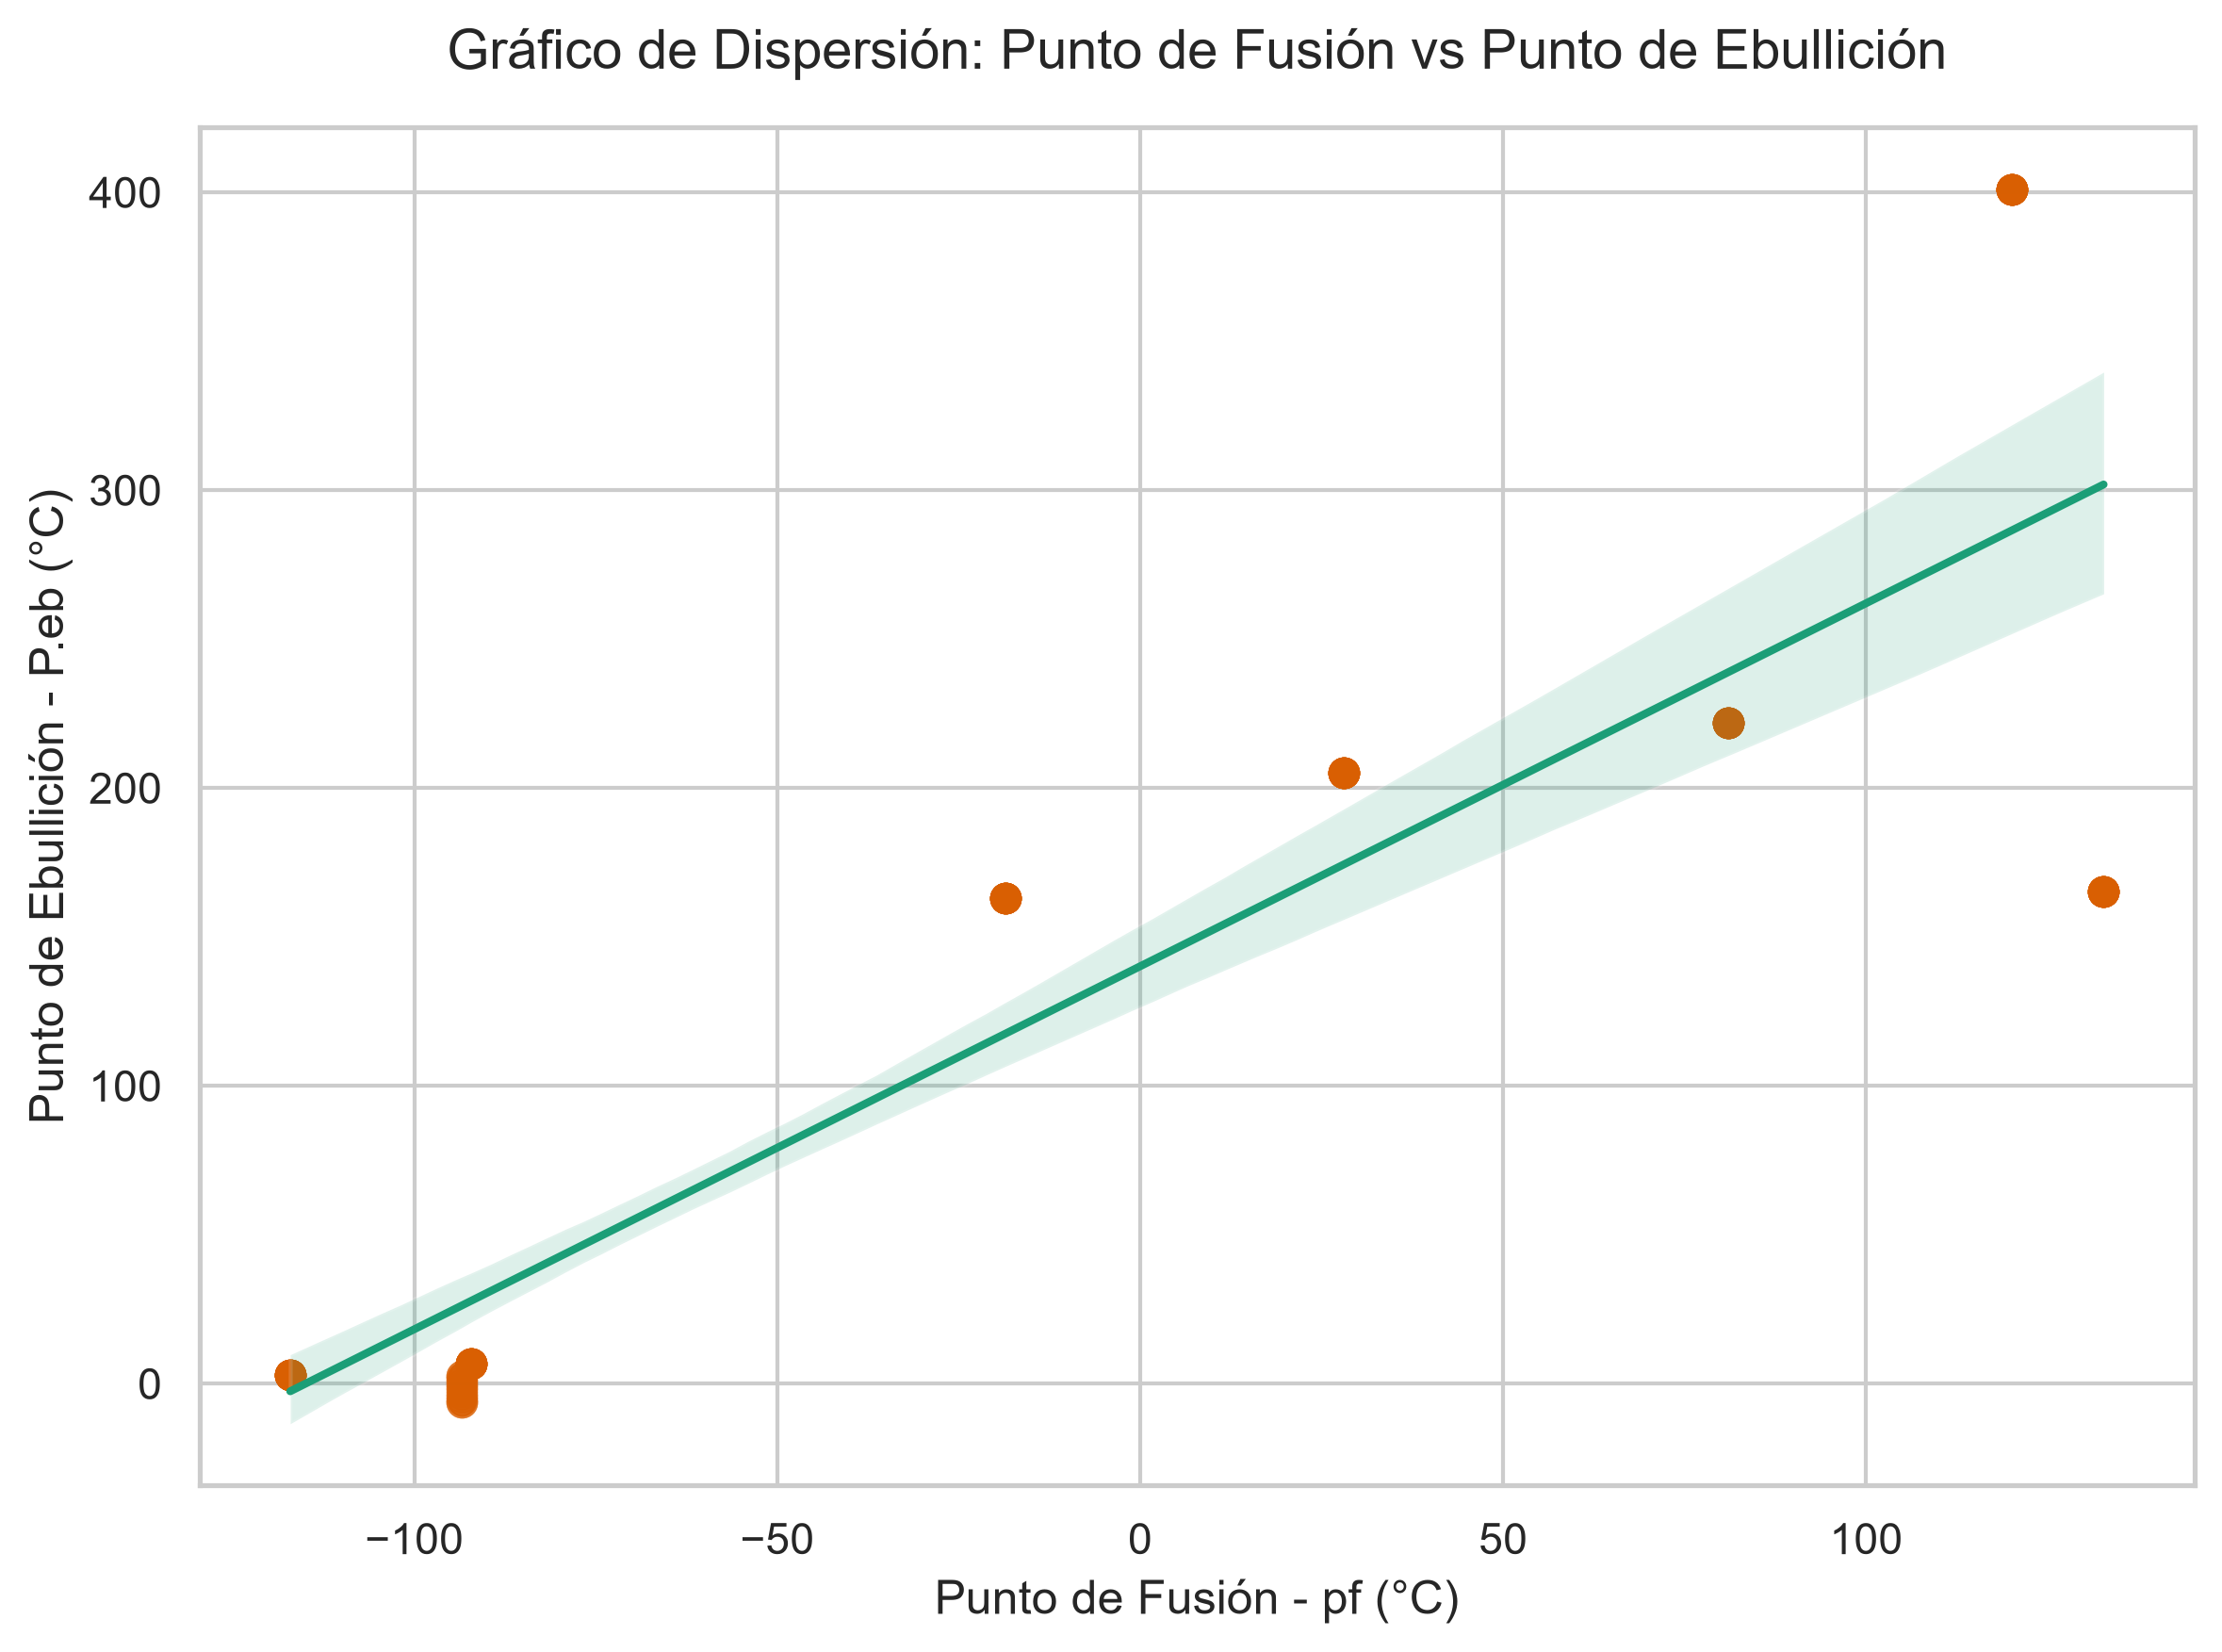
\includegraphics[width=\columnwidth]{05_reg_pf_vs_peb.png}
	\caption{Punto de fusión frente a punto de ebullición.}
	\label{fig:pf-peb}
\end{figure}

\begin{figure}[htbp]
	\centering
	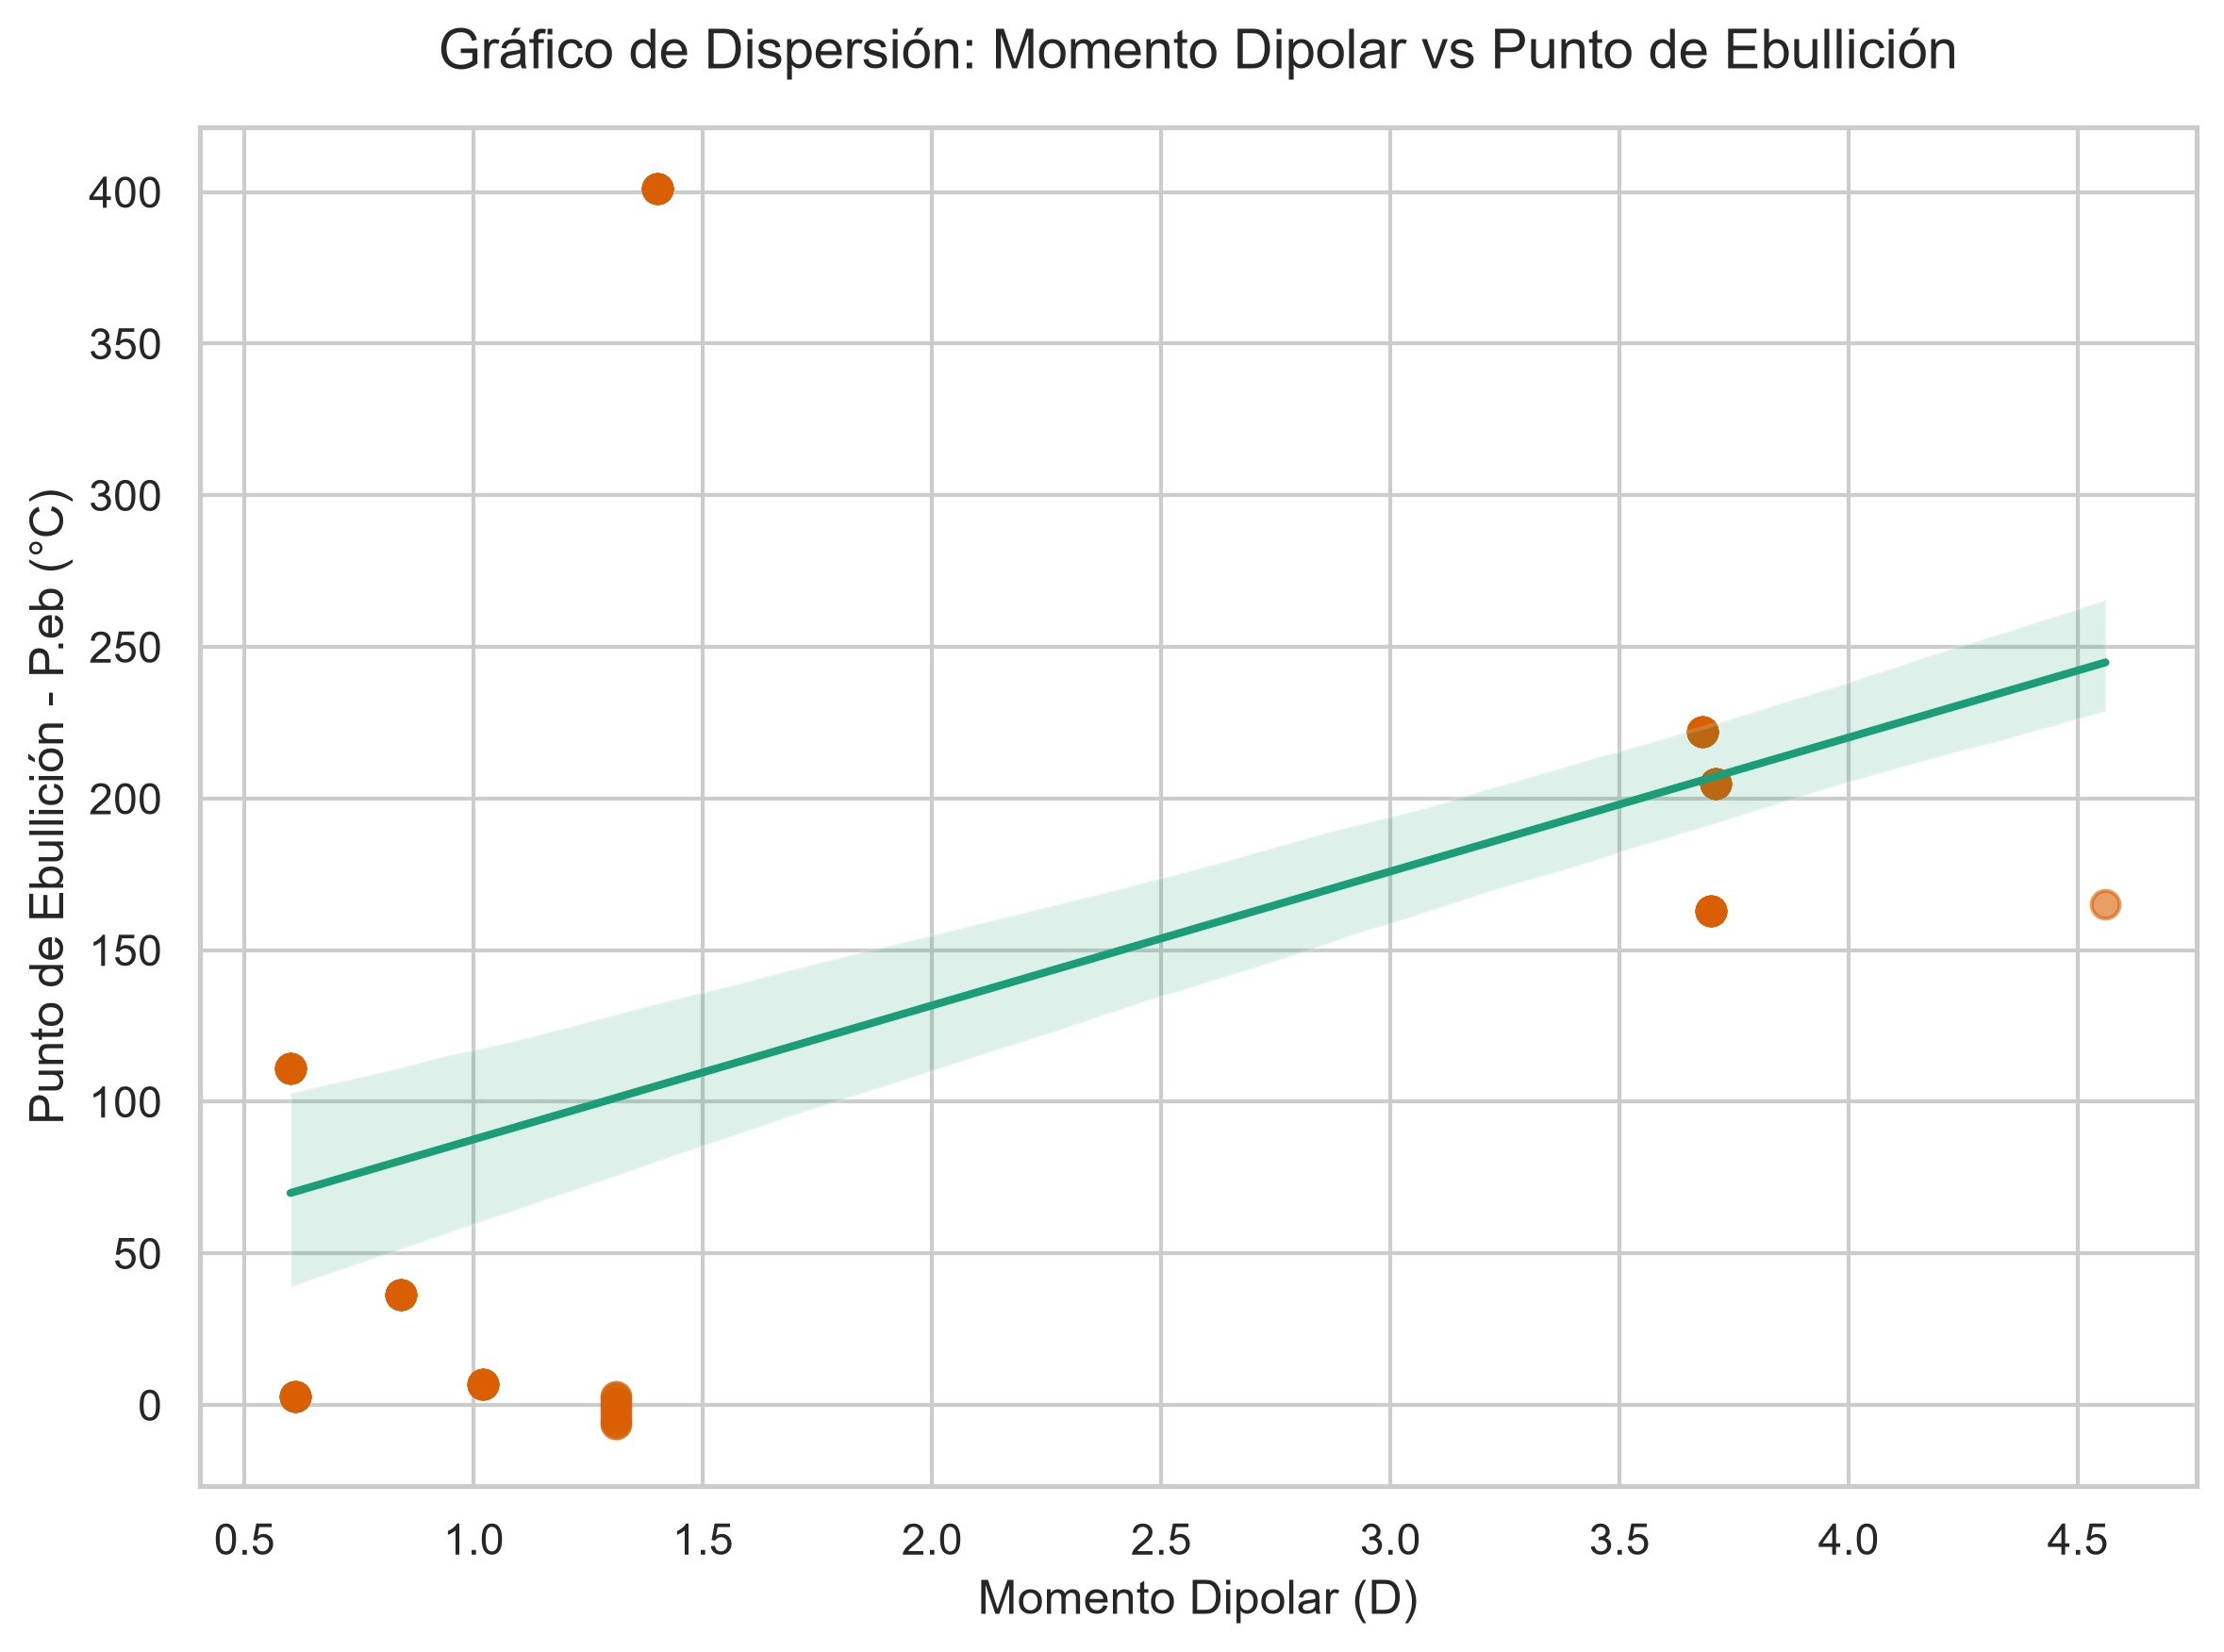
\includegraphics[width=\columnwidth]{06_reg_dipolo_vs_peb.png}
	\caption{Momento dipolar frente a punto de ebullición.}
	\label{fig:dip-peb}
\end{figure}

\subsection{Exploración interactiva con Plotly}
% TODO (Valentina): interpretar; idea central: a igual PM, los compuestos con
% enlace N--H (donadores de puente de H) hierven mucho más alto.
Las Figuras~\ref{fig:burbujas}--\ref{fig:dens-sol} se generaron con Plotly,
una fila por compuesto; sus versiones HTML permiten inspeccionar cada molécula
con el cursor. En la Figura~\ref{fig:burbujas}, trimetilamina
(\SI{2.8}{\degreeCelsius}) y N-metiletanamina (\SI{36.5}{\degreeCelsius}) tienen
el mismo peso molecular (\SI{59.11}{\gram\per\mole}): la diferencia se debe a que
sólo la segunda posee enlace N--H y forma puentes de hidrógeno.
\textit{[Interpretación pendiente.]}

\begin{figure}[htbp]
	\centering
	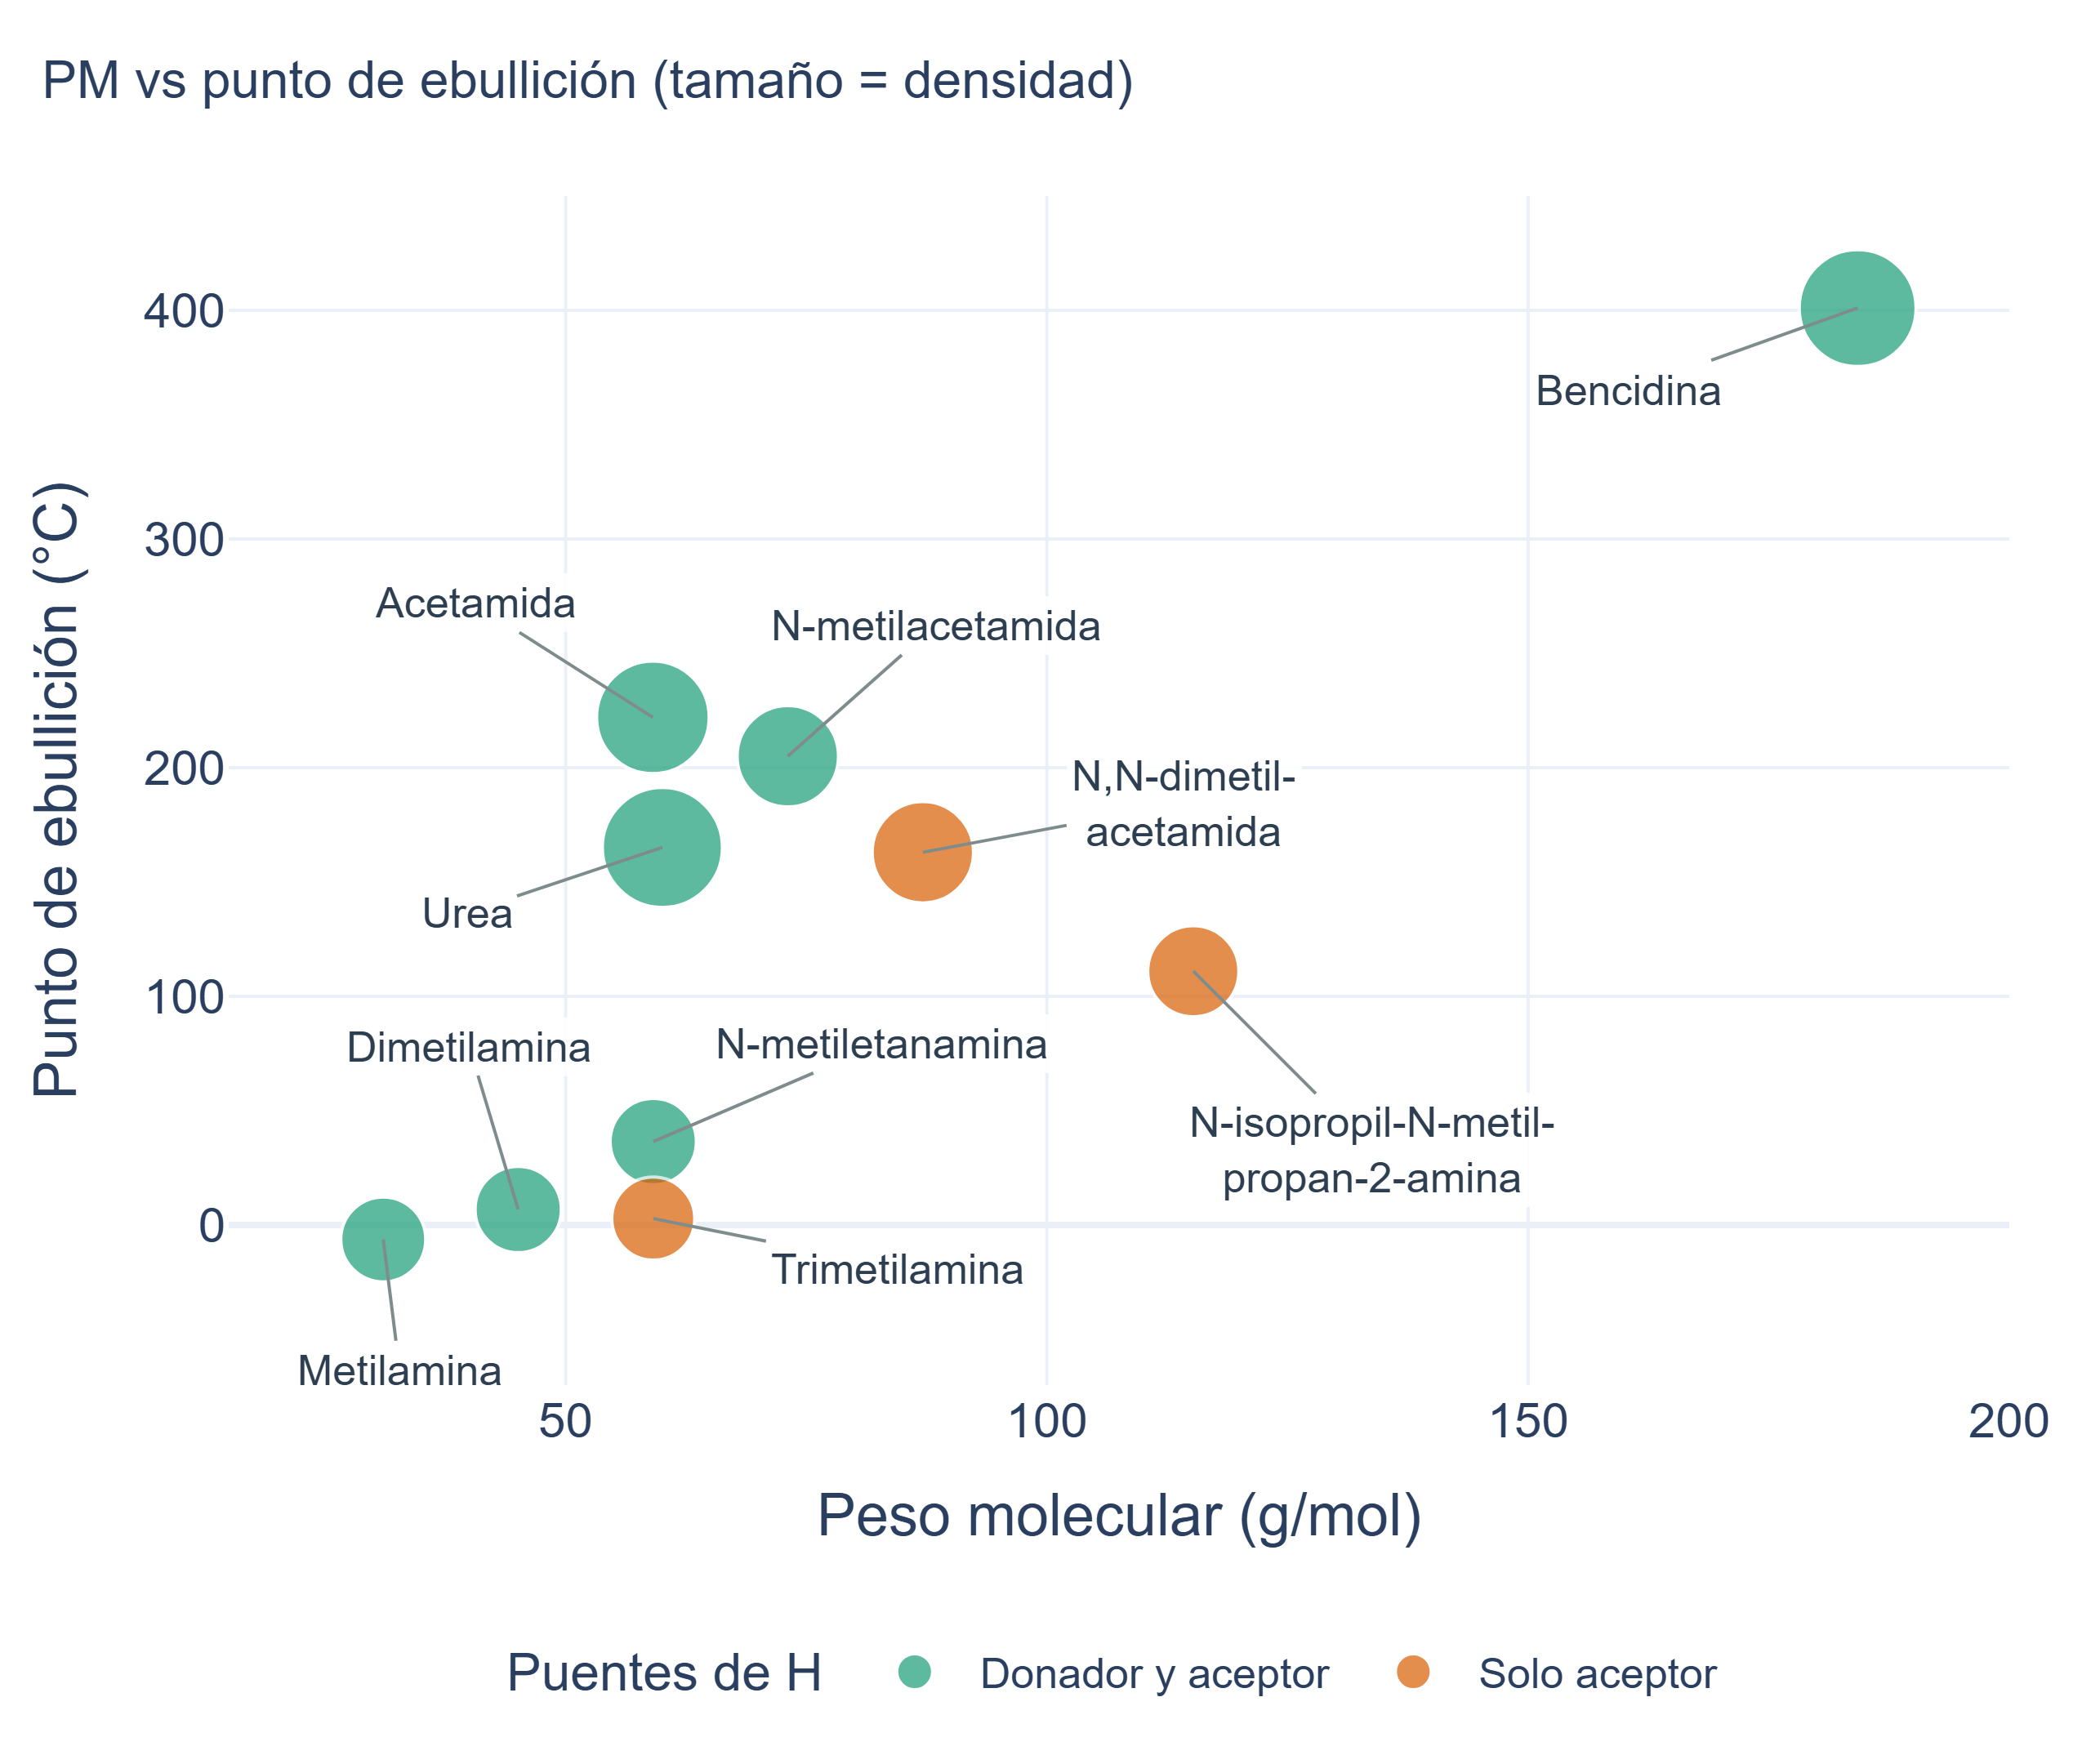
\includegraphics[width=\columnwidth]{11_plotly_burbujas_pm_peb.png}
	\caption{Peso molecular frente a punto de ebullición; el tamaño representa la densidad y el color la capacidad de formar puentes de hidrógeno.}
	\label{fig:burbujas}
\end{figure}

\begin{figure}[htbp]
	\centering
	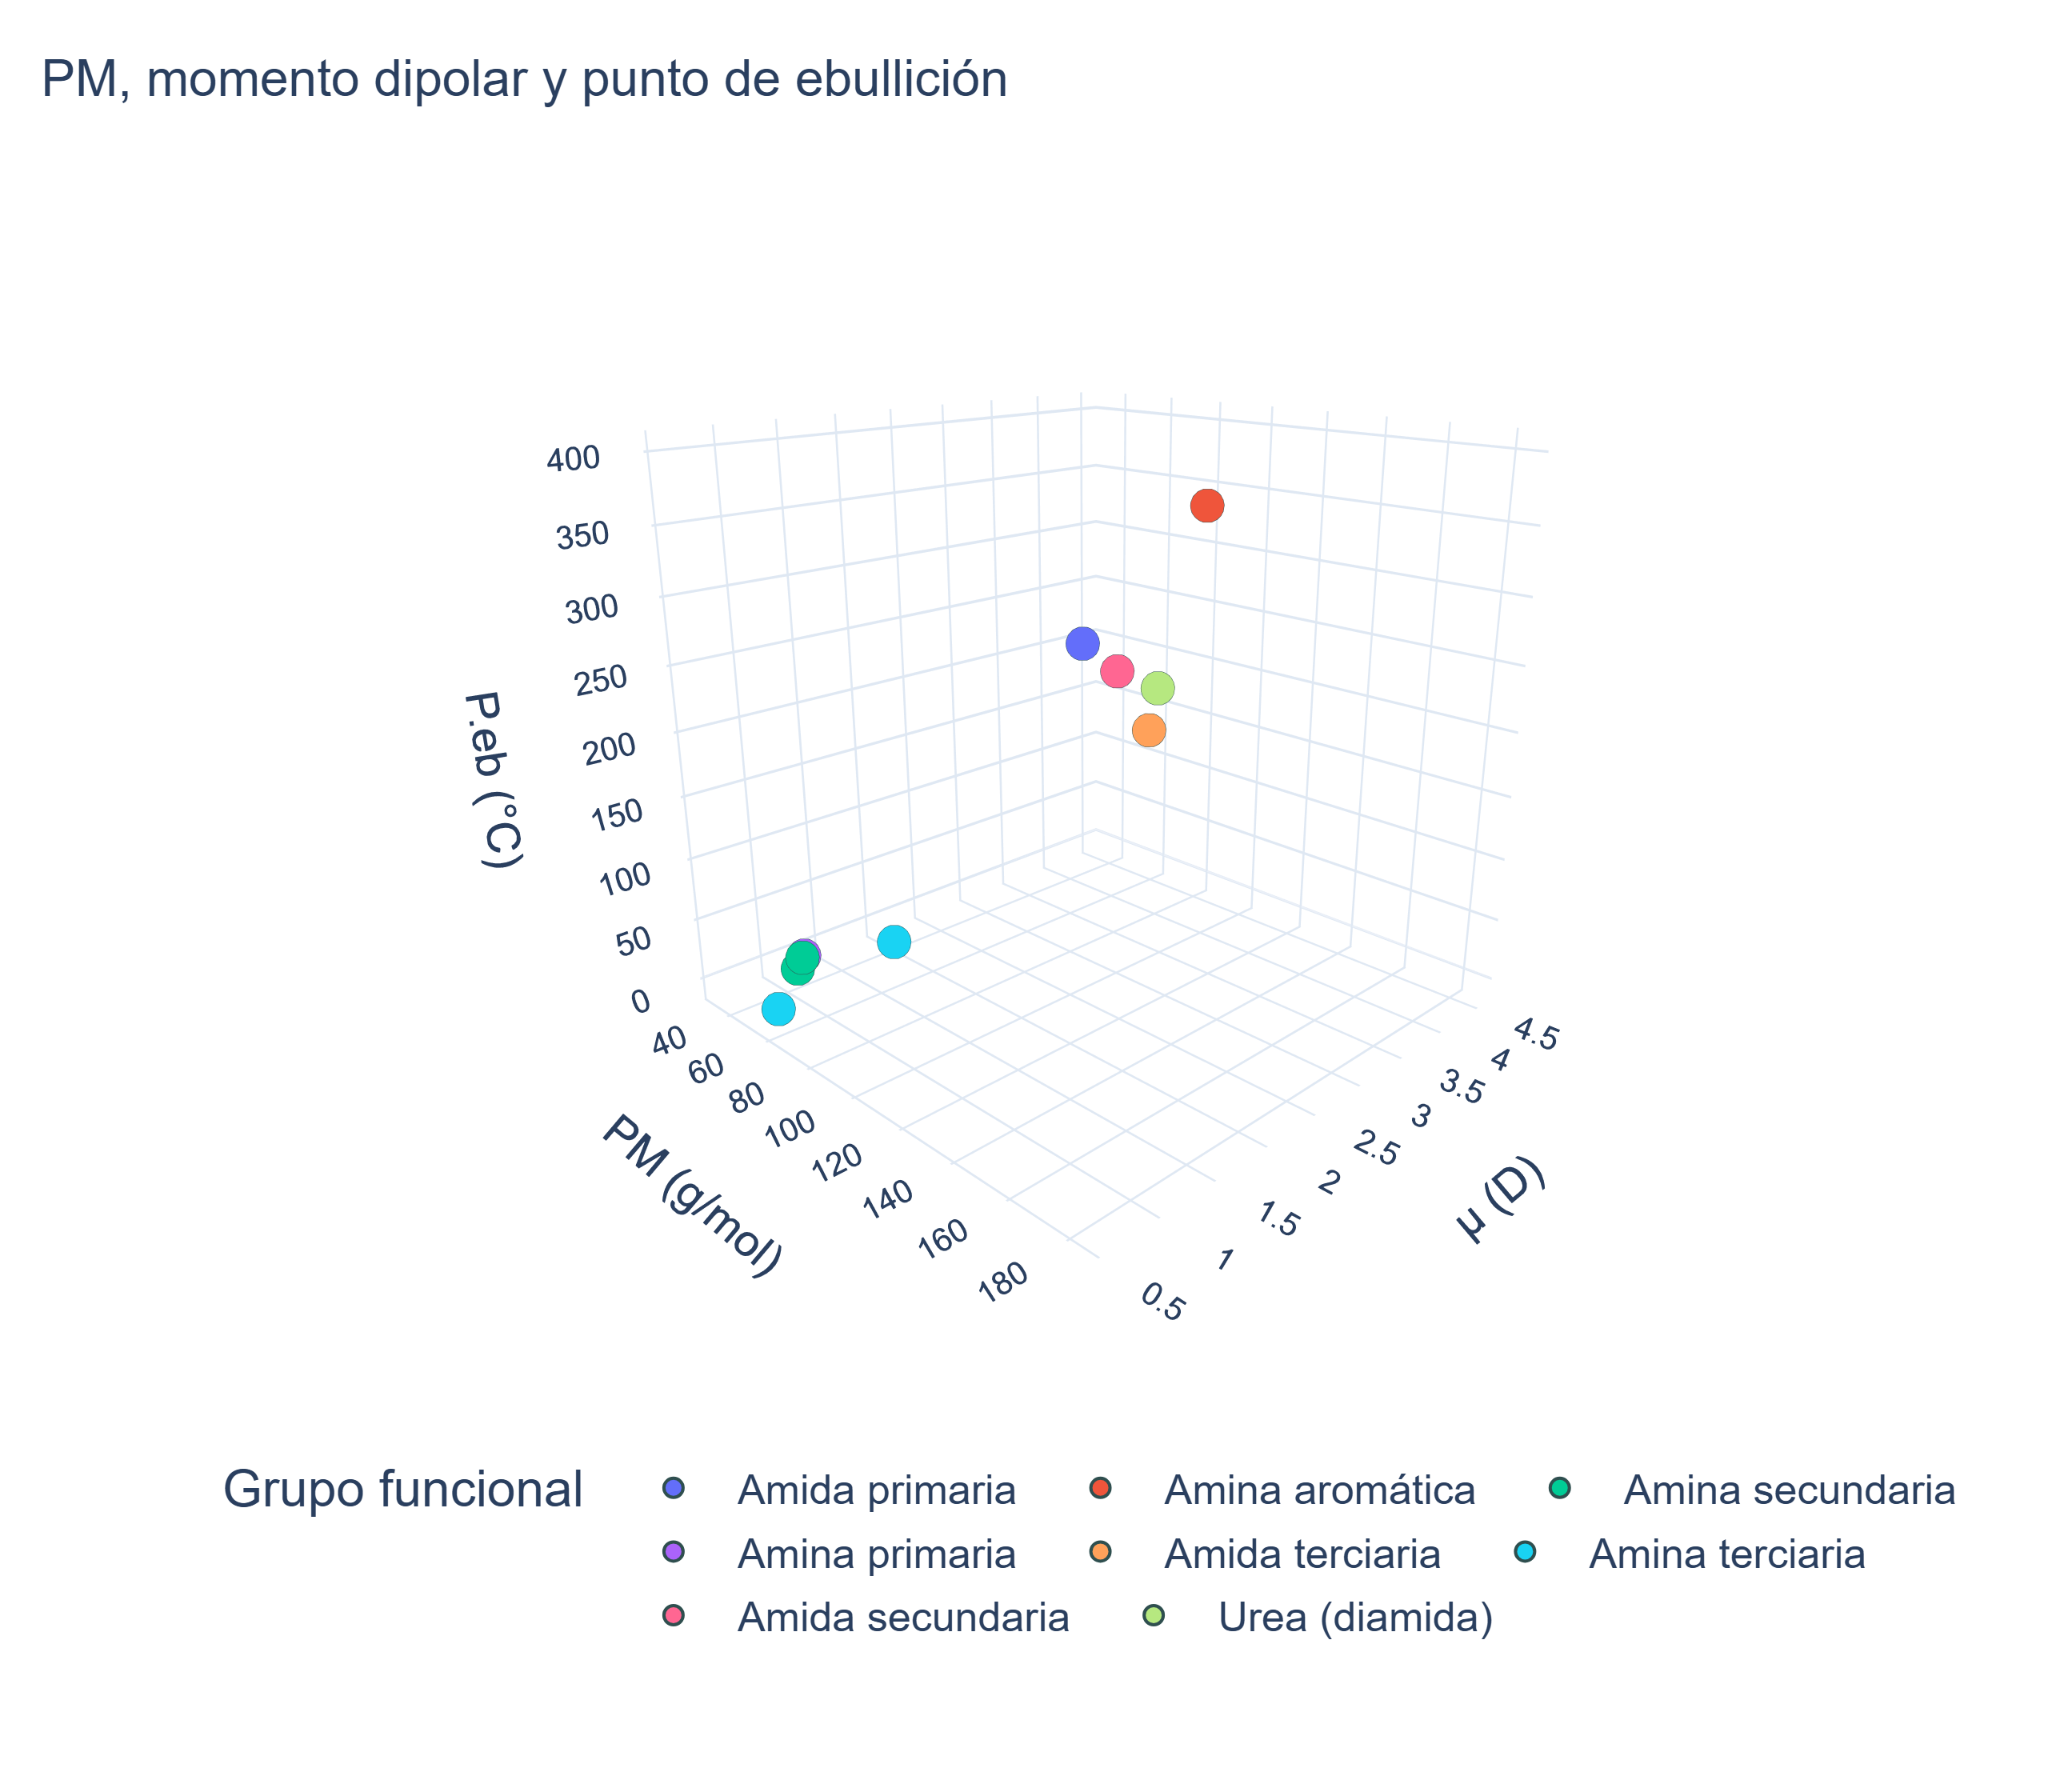
\includegraphics[width=\columnwidth]{12_plotly_3d_pm_dipolo_peb.png}
	\caption{Espacio tridimensional de peso molecular, momento dipolar y punto de ebullición por grupo funcional.}
	\label{fig:3d}
\end{figure}

\begin{figure}[htbp]
	\centering
	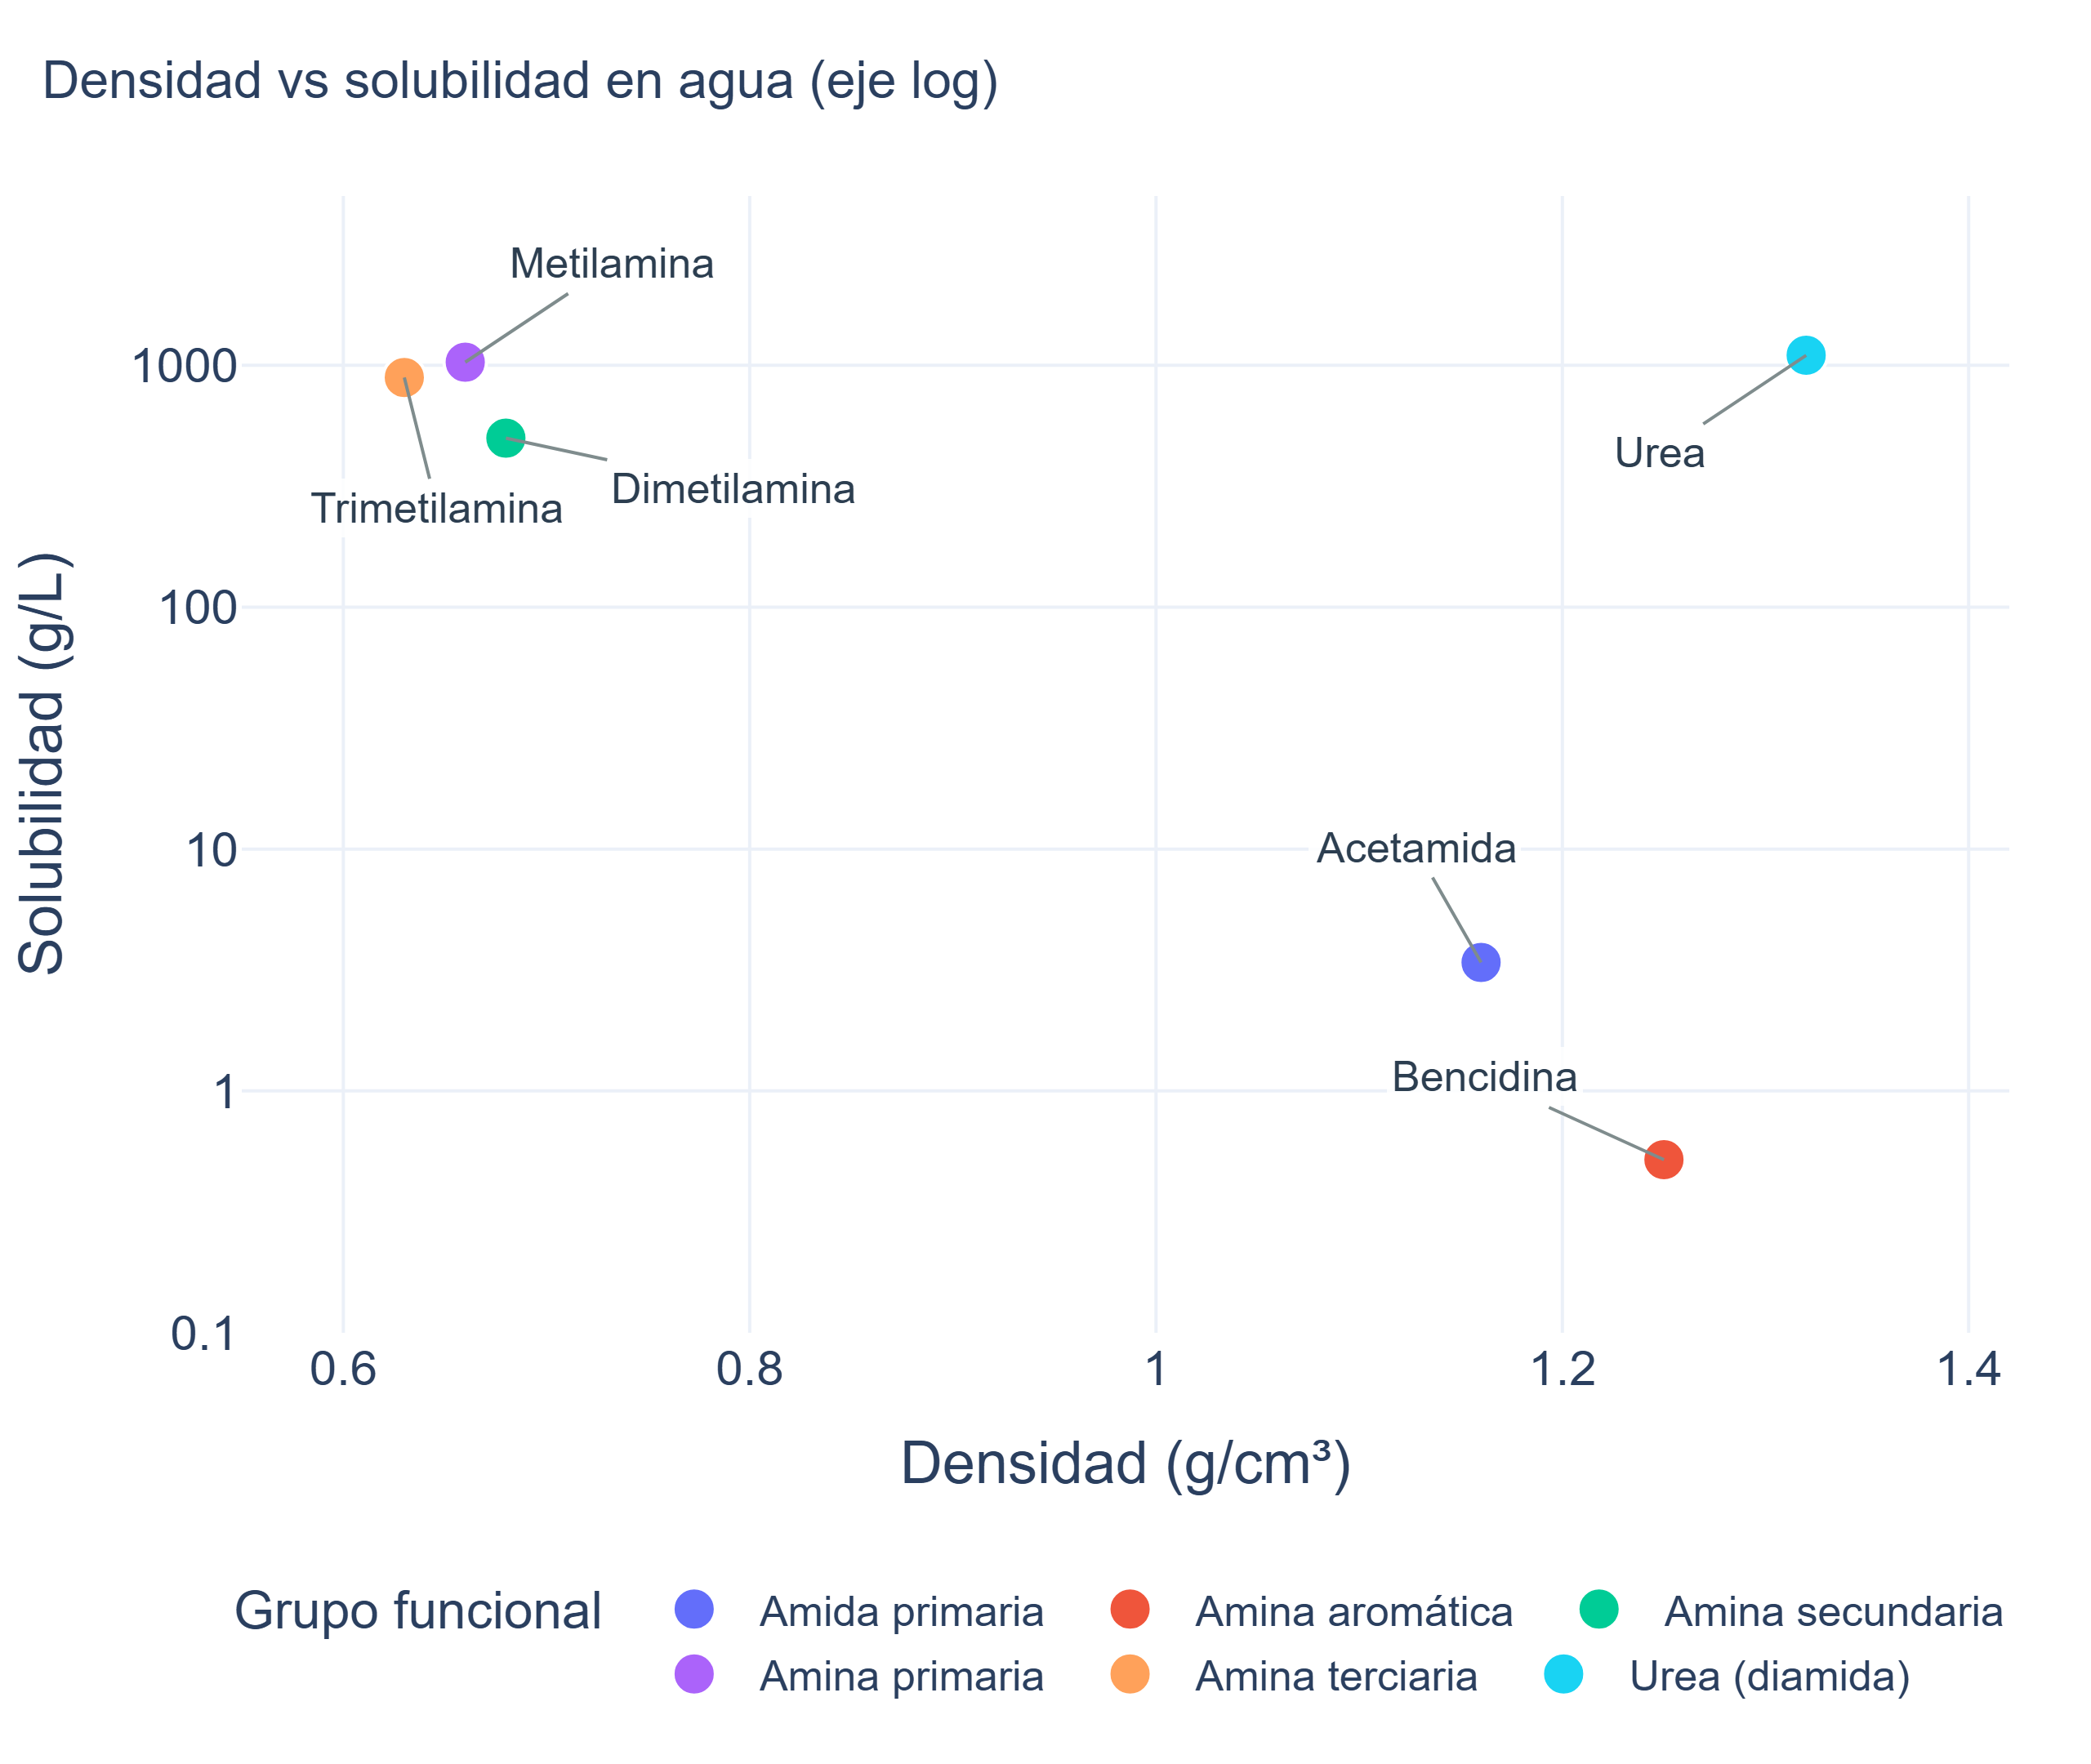
\includegraphics[width=\columnwidth]{13_plotly_densidad_solubilidad.png}
	\caption{Densidad frente a solubilidad en agua (eje logarítmico).}
	\label{fig:dens-sol}
\end{figure}

\subsection{Distribución por tipo de reacción y medio}
% TODO (Valentina): explicar qué representa TR y comparar medianas/dispersiones.
La Figura~\ref{fig:frecuencias} compara la frecuencia de cada mecanismo de
reacción y de cada medio; la sustitución nucleofílica (SN) domina, coherente con
el carácter nucleófilo del par libre del nitrógeno. Las
Figuras~\ref{fig:violin}--\ref{fig:dona} describen la distribución de
probabilidad de TR según el tipo de reacción y el medio.
\textit{[Interpretación pendiente.]}

\begin{figure}[htbp]
	\centering
	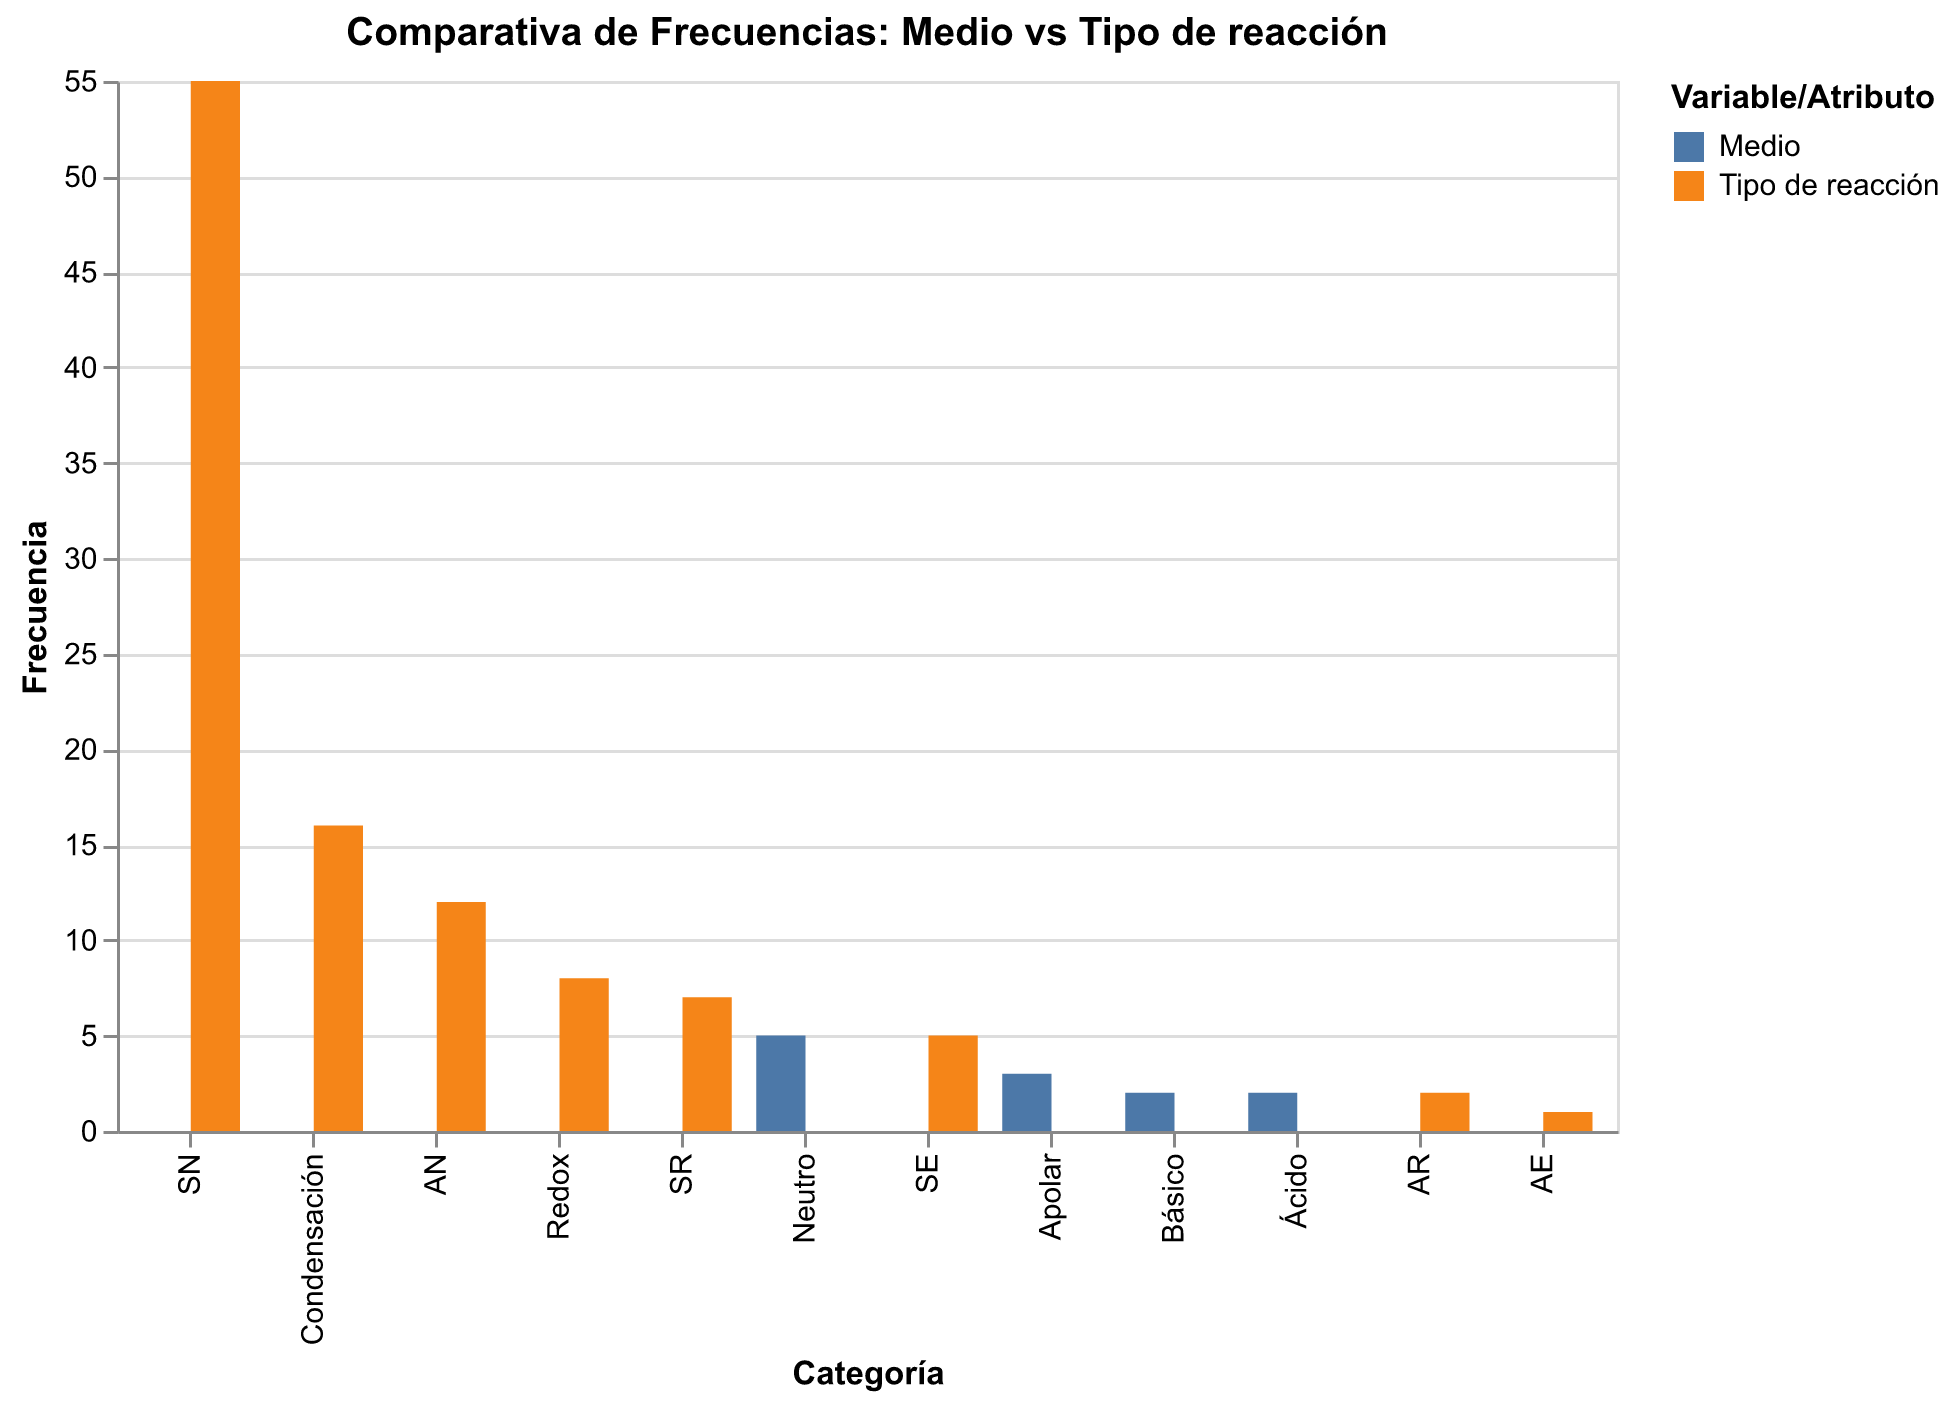
\includegraphics[width=\columnwidth]{09_frecuencias_medio_tipo.png}
	\caption{Frecuencia de los tipos de reacción y de los medios reportados.}
	\label{fig:frecuencias}
\end{figure}

\begin{figure}[htbp]
	\centering
	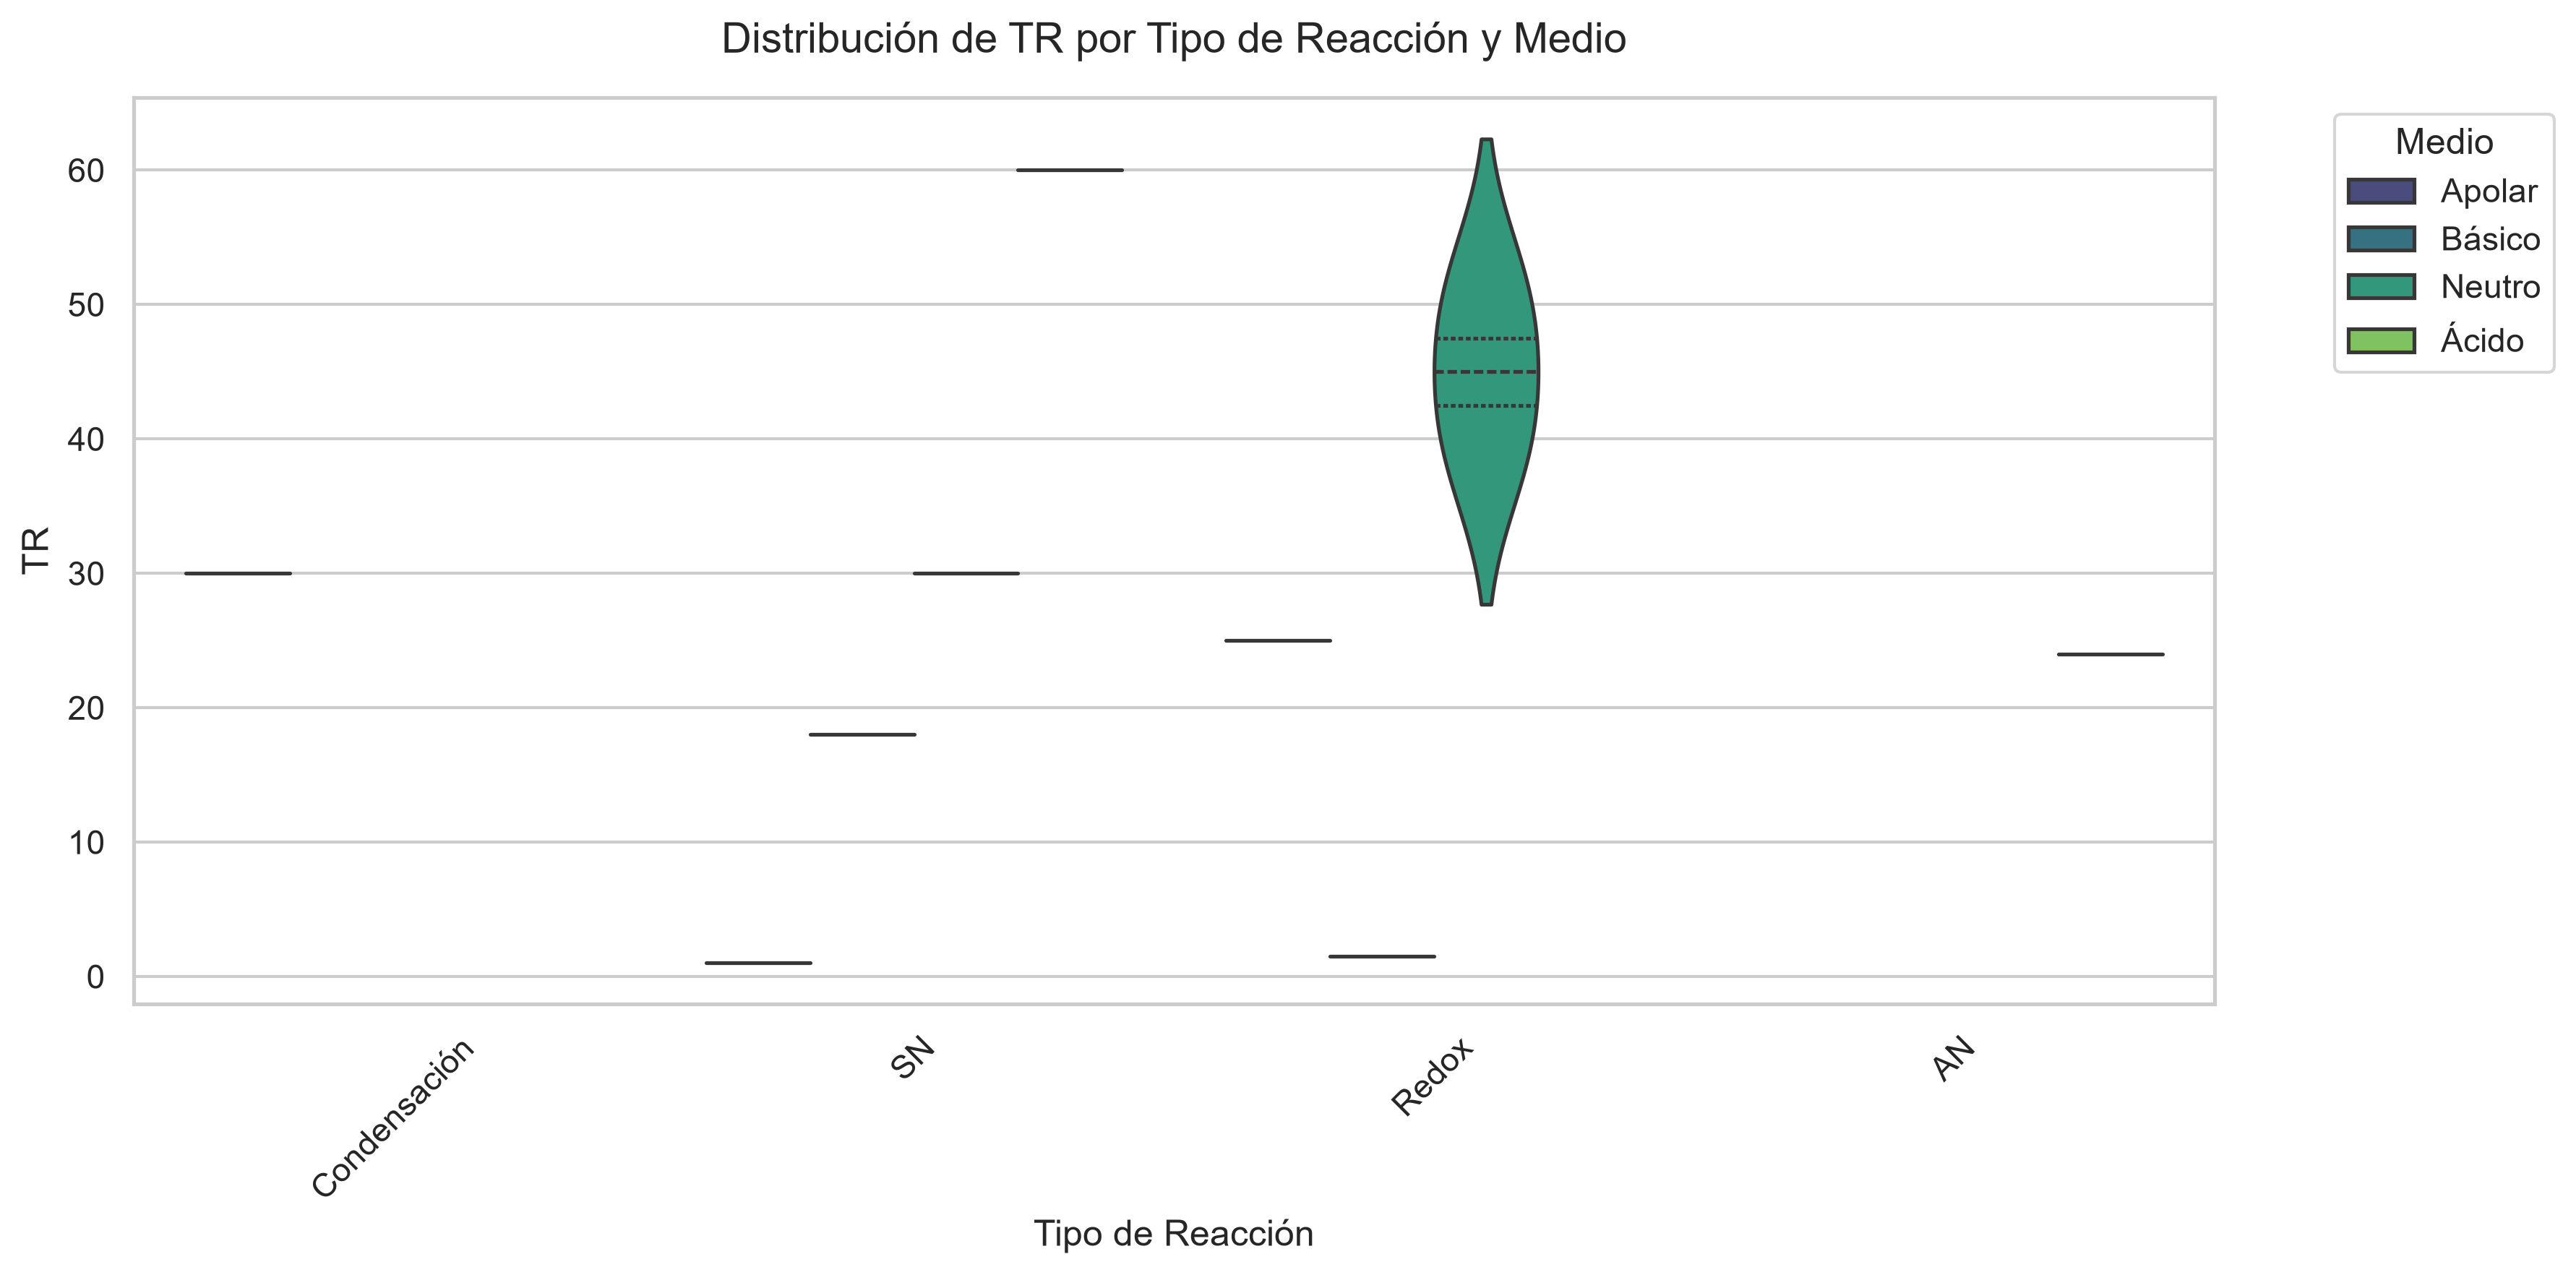
\includegraphics[width=\columnwidth]{07_violin_TR_tipo_medio.png}
	\caption{Distribución (violín) de TR por tipo de reacción y medio.}
	\label{fig:violin}
\end{figure}

\begin{figure}[htbp]
	\centering
	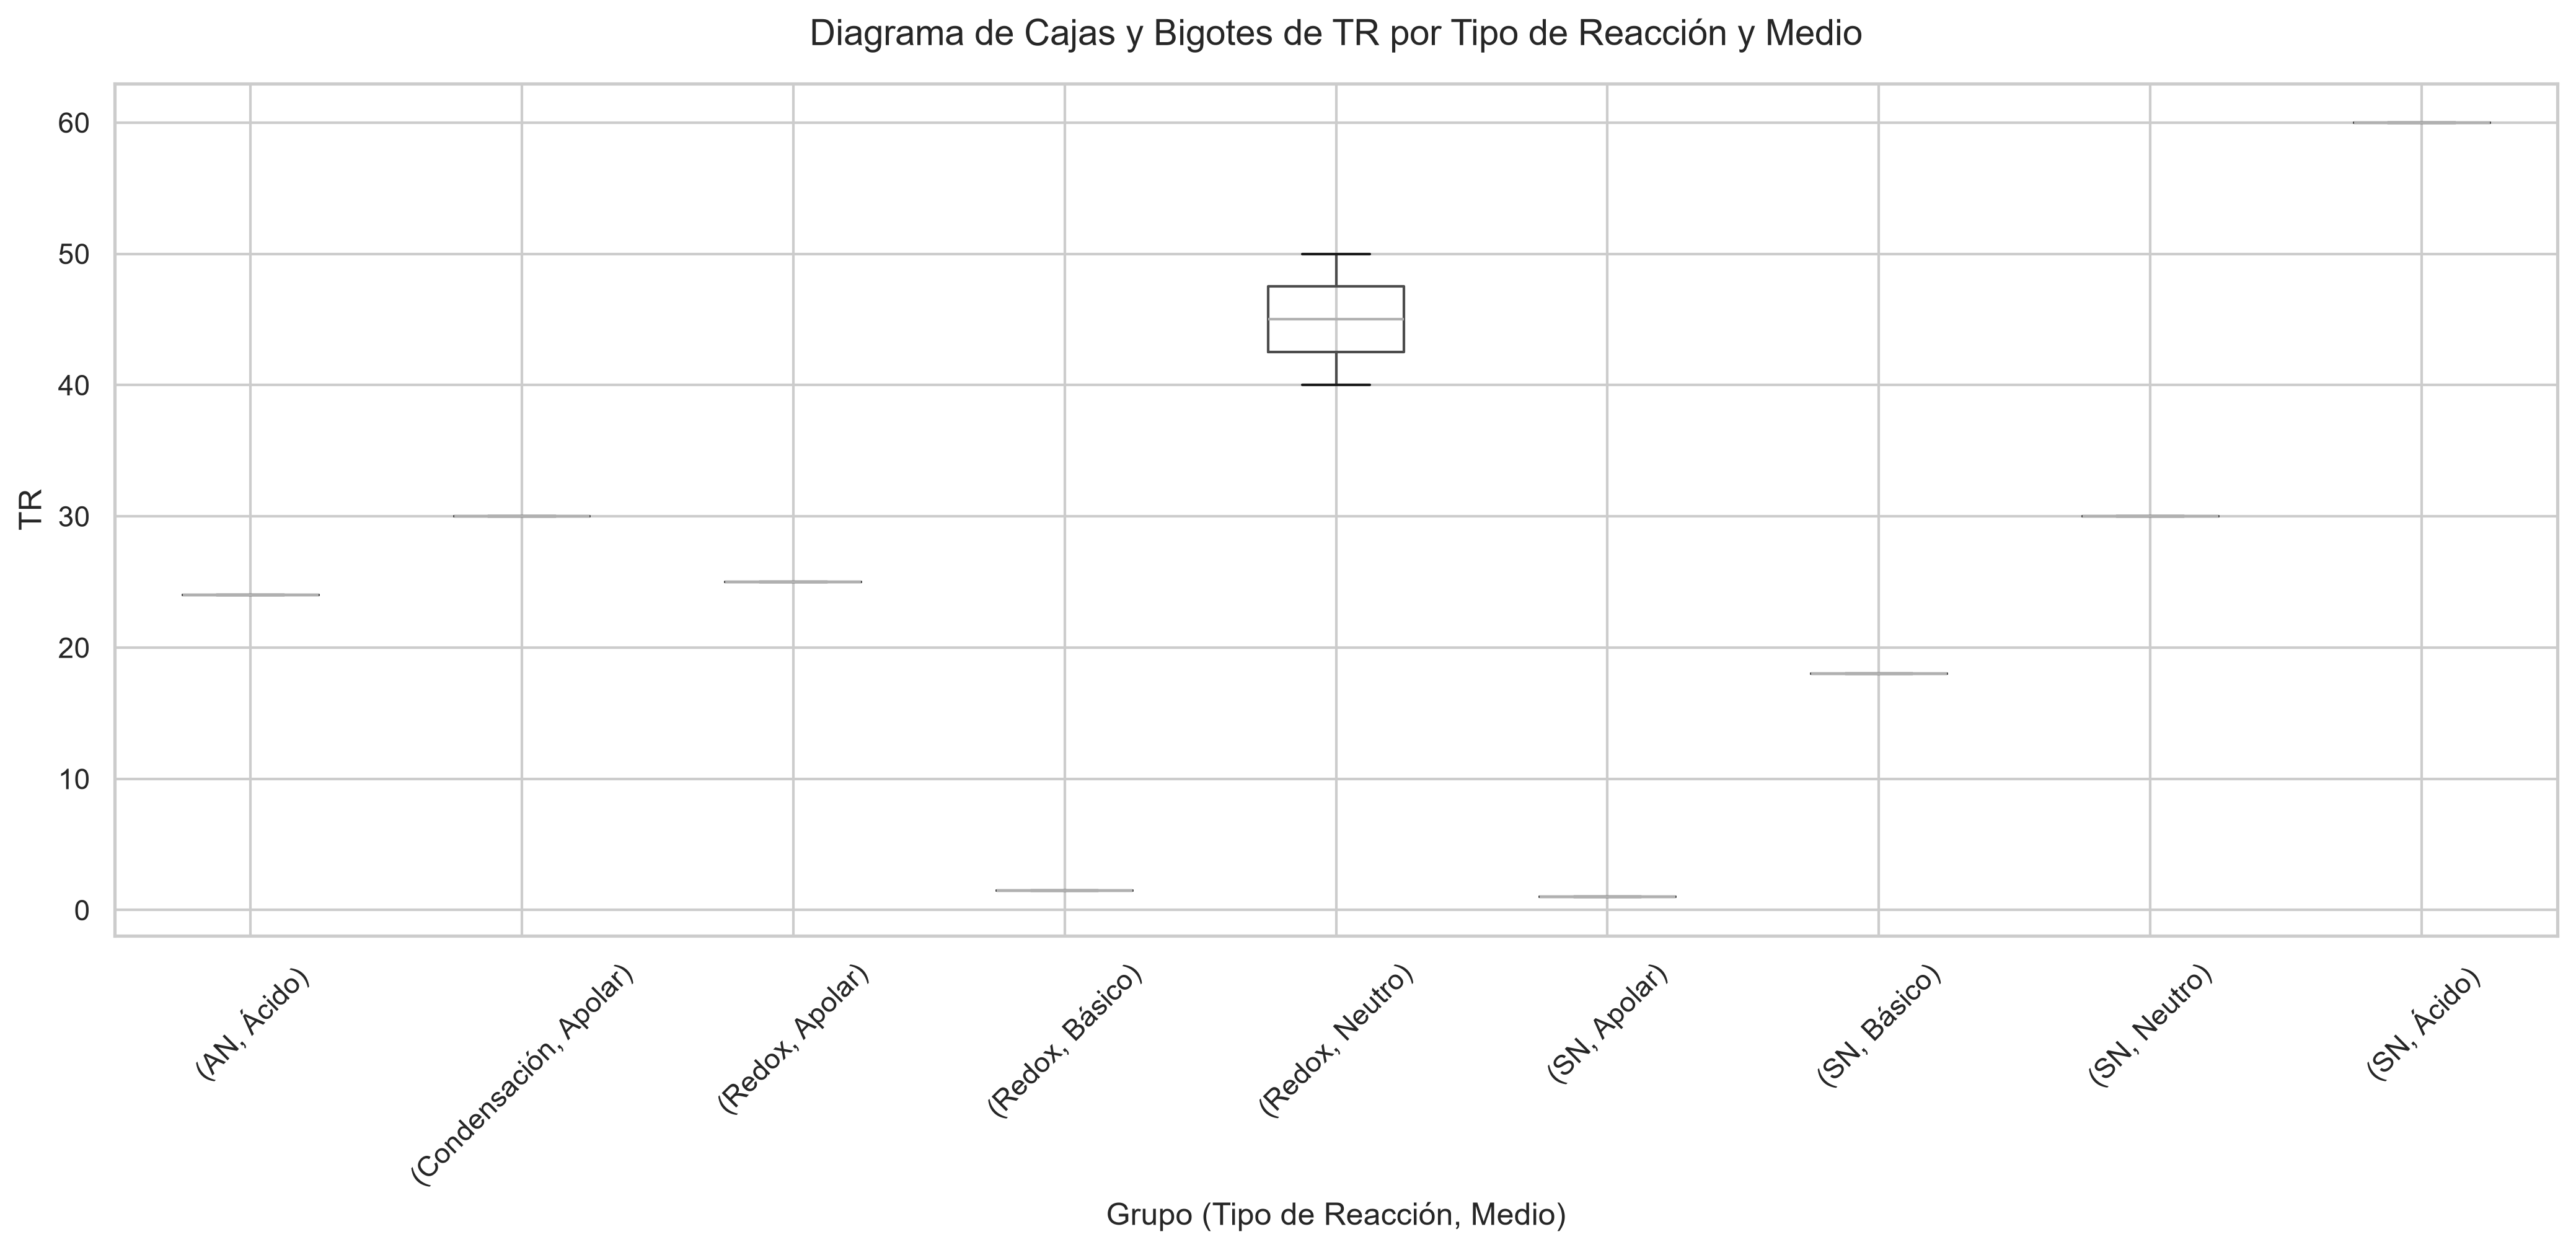
\includegraphics[width=\columnwidth]{08_boxplot_TR_tipo_medio.png}
	\caption{Diagrama de cajas y bigotes de TR por tipo de reacción y medio.}
	\label{fig:boxplot}
\end{figure}

\begin{figure}[htbp]
	\centering
	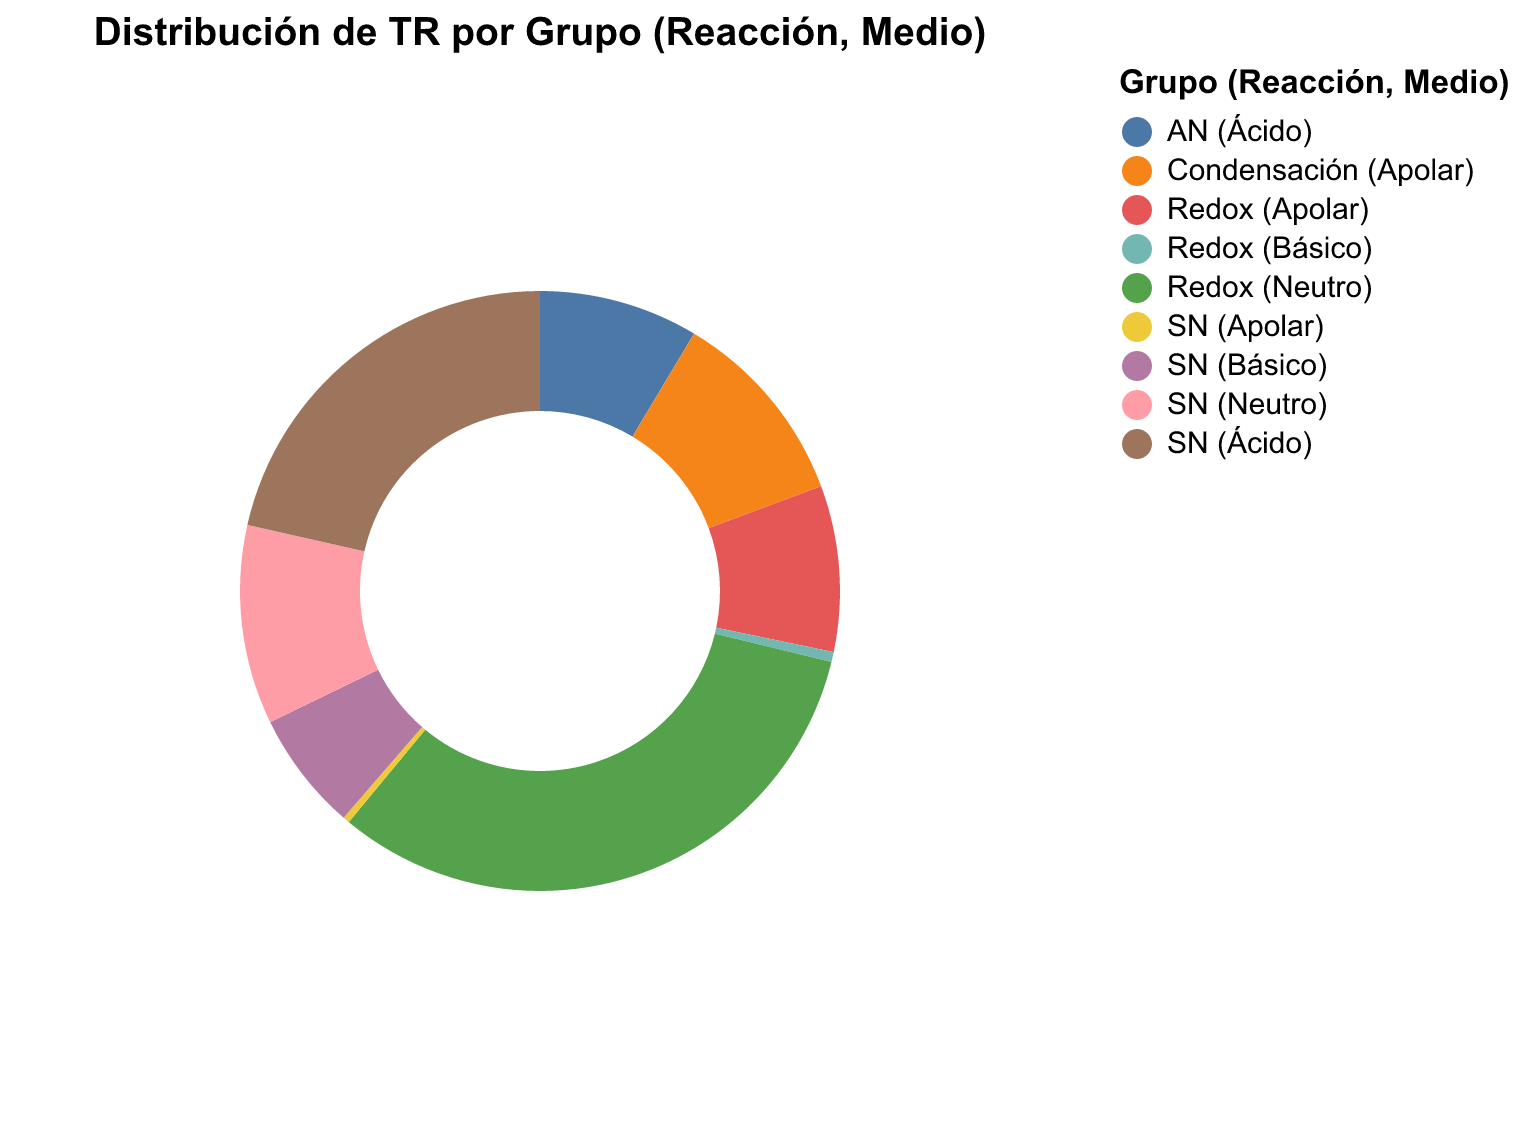
\includegraphics[width=0.9\columnwidth]{10_dona_TR_grupo.png}
	\caption{Participación de TR por grupo (tipo de reacción, medio).}
	\label{fig:dona}
\end{figure}

\section{Conclusiones y Perspectiva}
\fontsize{12}{14}\selectfont
% TODO (Valentina): 3--5 conclusiones que respondan al objetivo de la introducción,
% cada una sustentada en una figura o en la Tabla~\ref{tab:propiedades}.
\textit{[Redacción pendiente.]}

%  Contenido: Metodología, Análisis Gráfico (Colab/Conda) y Conclusiones
%
%  Reglas para editar sin romper la compilación:
%   * NO escribir \documentclass, \begin{document} ni \end{document} aquí.
%   * Las figuras están en ../imagenes/ y se llaman sólo por su nombre
%     (main.tex ya define \graphicspath{{imagenes/}}).
%   * Referenciar figuras con Figura~\ref{fig:...}, nunca "la figura de abajo".
% =====================================================================

\section{Metodología}
\fontsize{12}{14}\selectfont
% TODO (Valentina): pegar aquí la redacción de la metodología.

\subsection{Recolección de datos}
\textit{[Redacción pendiente: búsqueda en CAS-SciFinder, compuestos e indicadores asignados, consolidación en Excel con formato Tabla.]}

\subsection{Limpieza y procesamiento en Python}
\textit{[Redacción pendiente: Google Colab con Pandas, NumPy, Matplotlib, Seaborn y Plotly; filtrado de los compuestos de interés, conversión de comas decimales, tratamiento de valores nulos y atípicos.]}

\subsection{Análisis estadístico}
\textit{[Redacción pendiente: correlación de Spearman (no paramétrica, robusta a valores atípicos y relaciones monótonas no lineales), regresiones lineales con intervalo de confianza del 95\,\% y distribuciones por tipo de reacción y medio.]}

\section{Resultados y Discusión}
\fontsize{12}{14}\selectfont

\subsection{Correlación entre propiedades}
% TODO (Valentina): interpretar los coeficientes más fuertes (positivos y negativos).
La Figura~\ref{fig:heatmap} presenta la matriz de correlación de Spearman entre
las propiedades fisicoquímicas, y la Figura~\ref{fig:clustermap} agrupa
jerárquicamente las variables con comportamiento similar.
\textit{[Interpretación pendiente.]}

\begin{figure}[htbp]
	\centering
	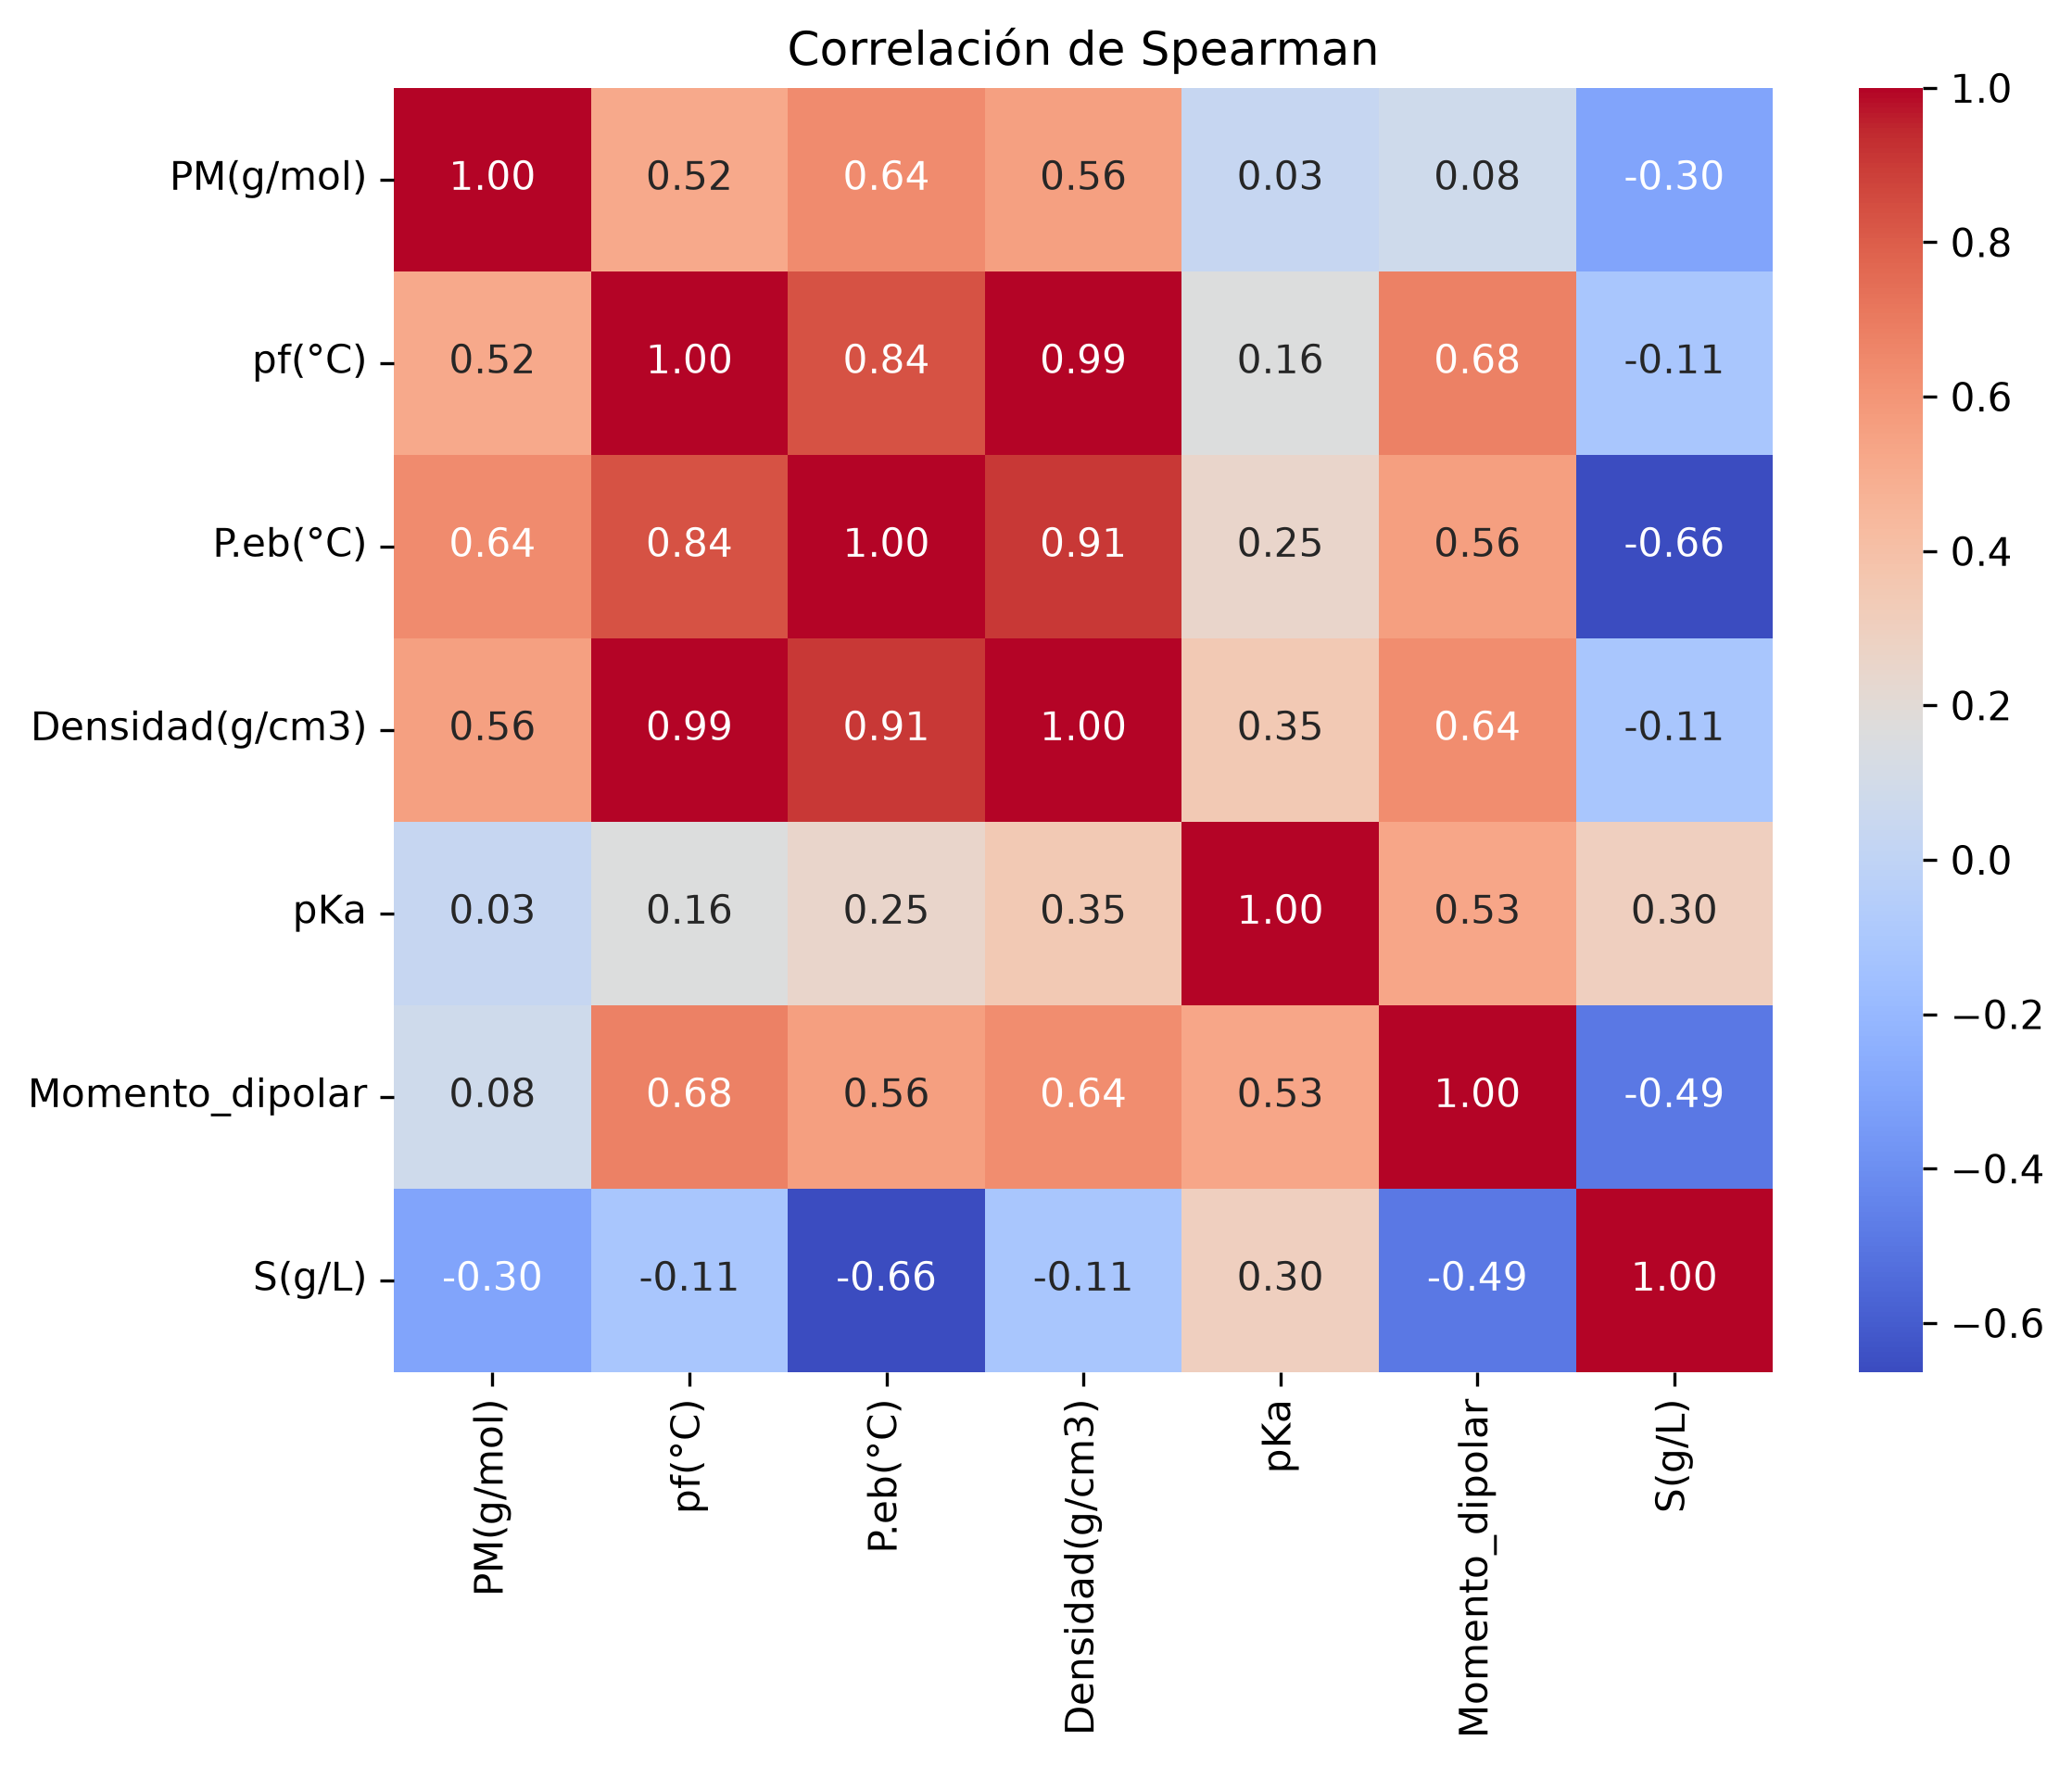
\includegraphics[width=\columnwidth]{01_heatmap_spearman.png}
	\caption{Matriz de correlación de Spearman entre las propiedades fisicoquímicas.}
	\label{fig:heatmap}
\end{figure}

\begin{figure}[htbp]
	\centering
	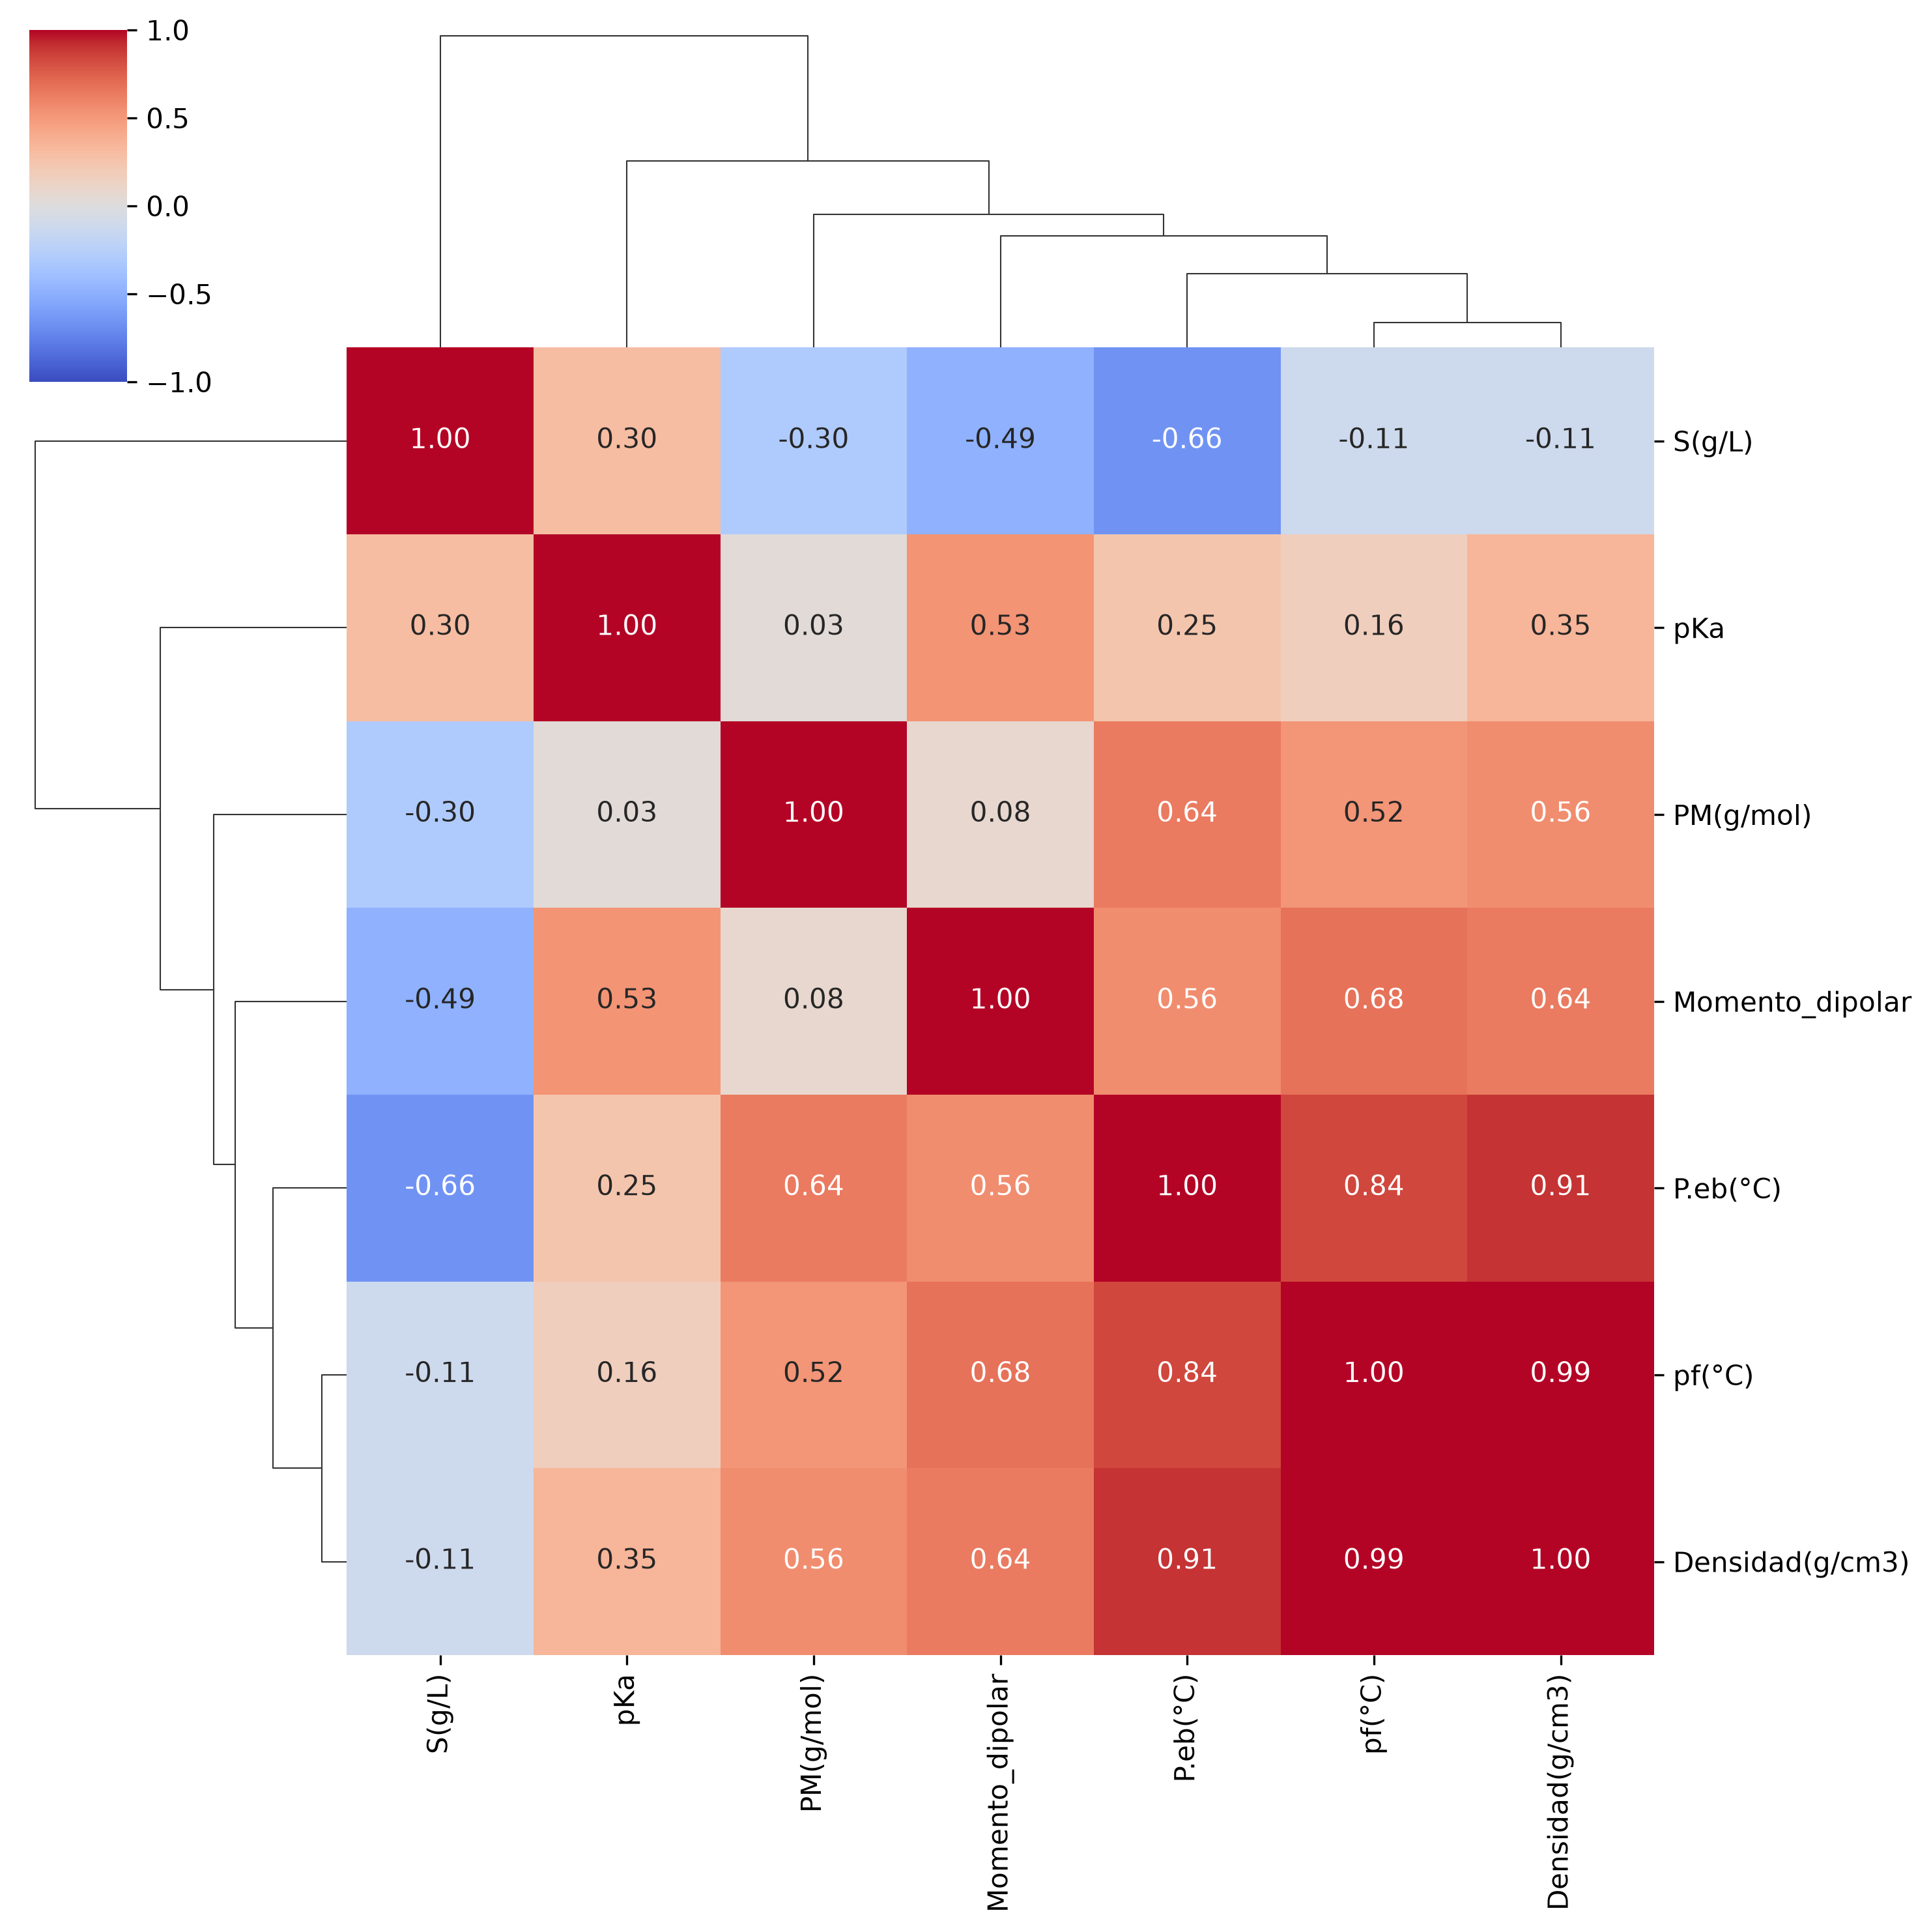
\includegraphics[width=\columnwidth]{02_clustermap_spearman.png}
	\caption{Mapa de agrupamiento jerárquico de la correlación de Spearman.}
	\label{fig:clustermap}
\end{figure}

\subsection{Tendencias entre propiedades}
% TODO (Valentina): discutir cada regresión en términos de fuerzas intermoleculares.
Las Figuras~\ref{fig:pf-dens}--\ref{fig:dip-peb} muestran las regresiones
lineales entre pares de propiedades, con su intervalo de confianza.
\textit{[Interpretación pendiente.]}

\begin{figure}[htbp]
	\centering
	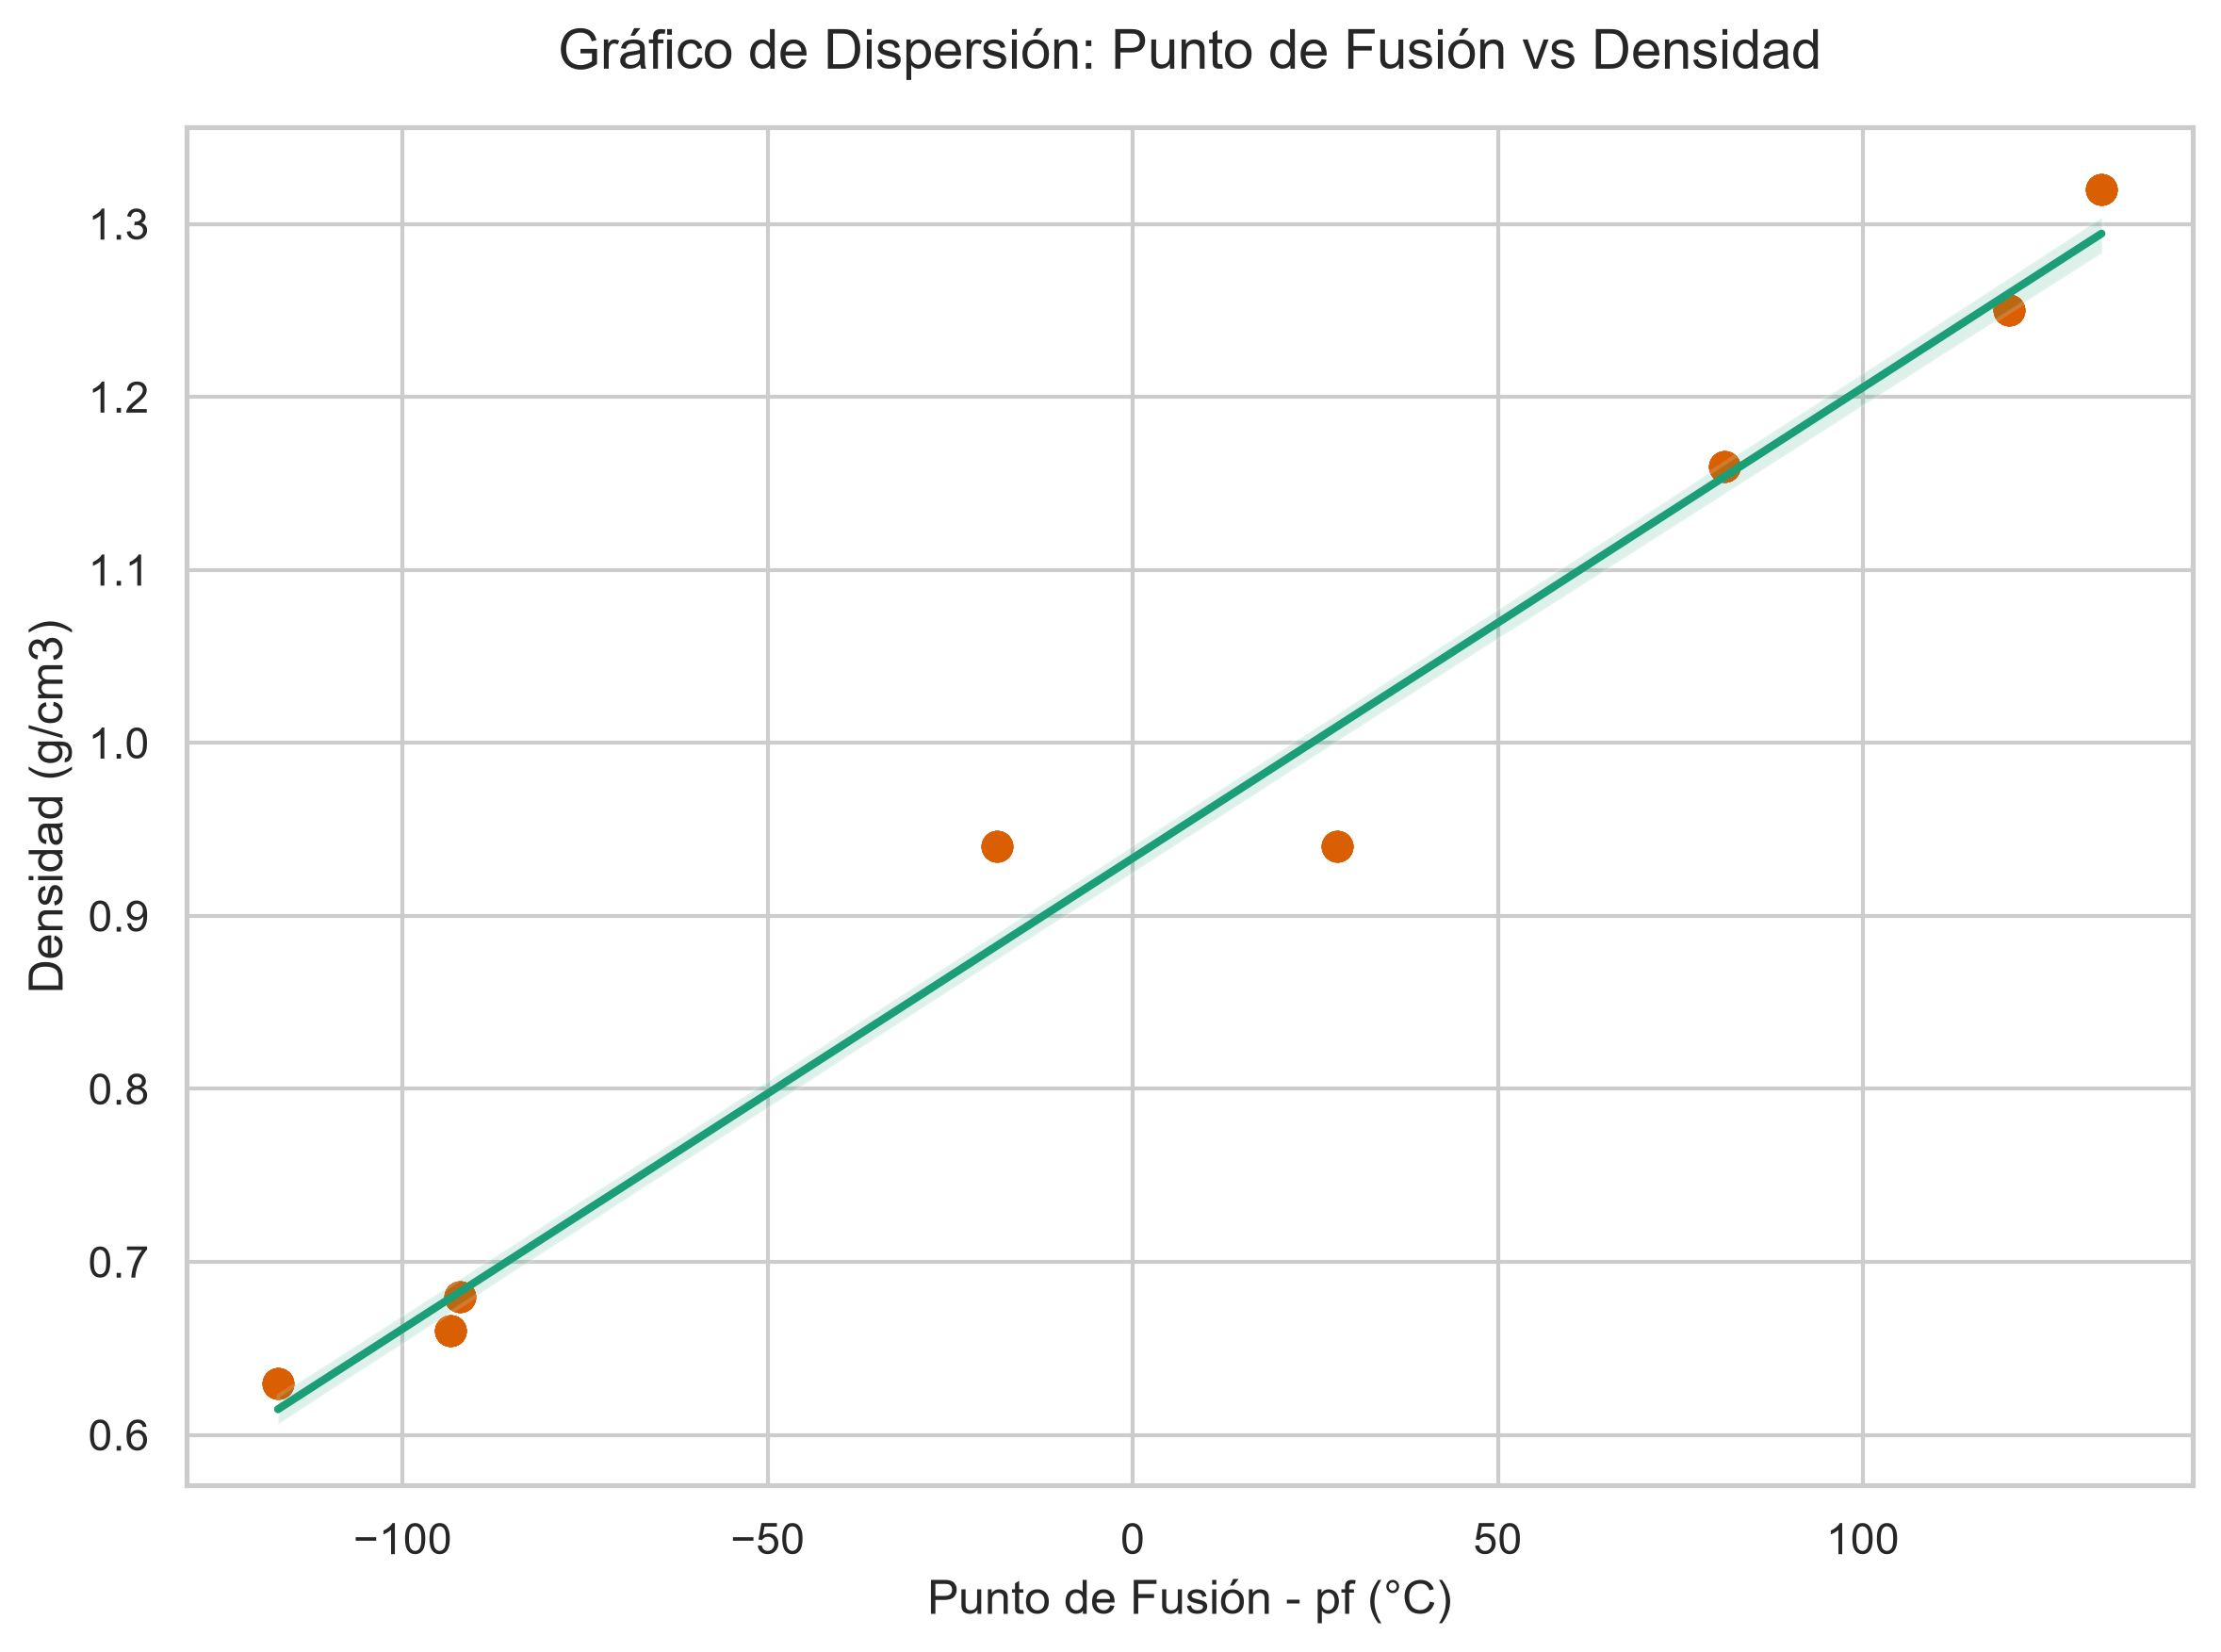
\includegraphics[width=\columnwidth]{03_reg_pf_vs_densidad.png}
	\caption{Punto de fusión frente a densidad.}
	\label{fig:pf-dens}
\end{figure}

\begin{figure}[htbp]
	\centering
	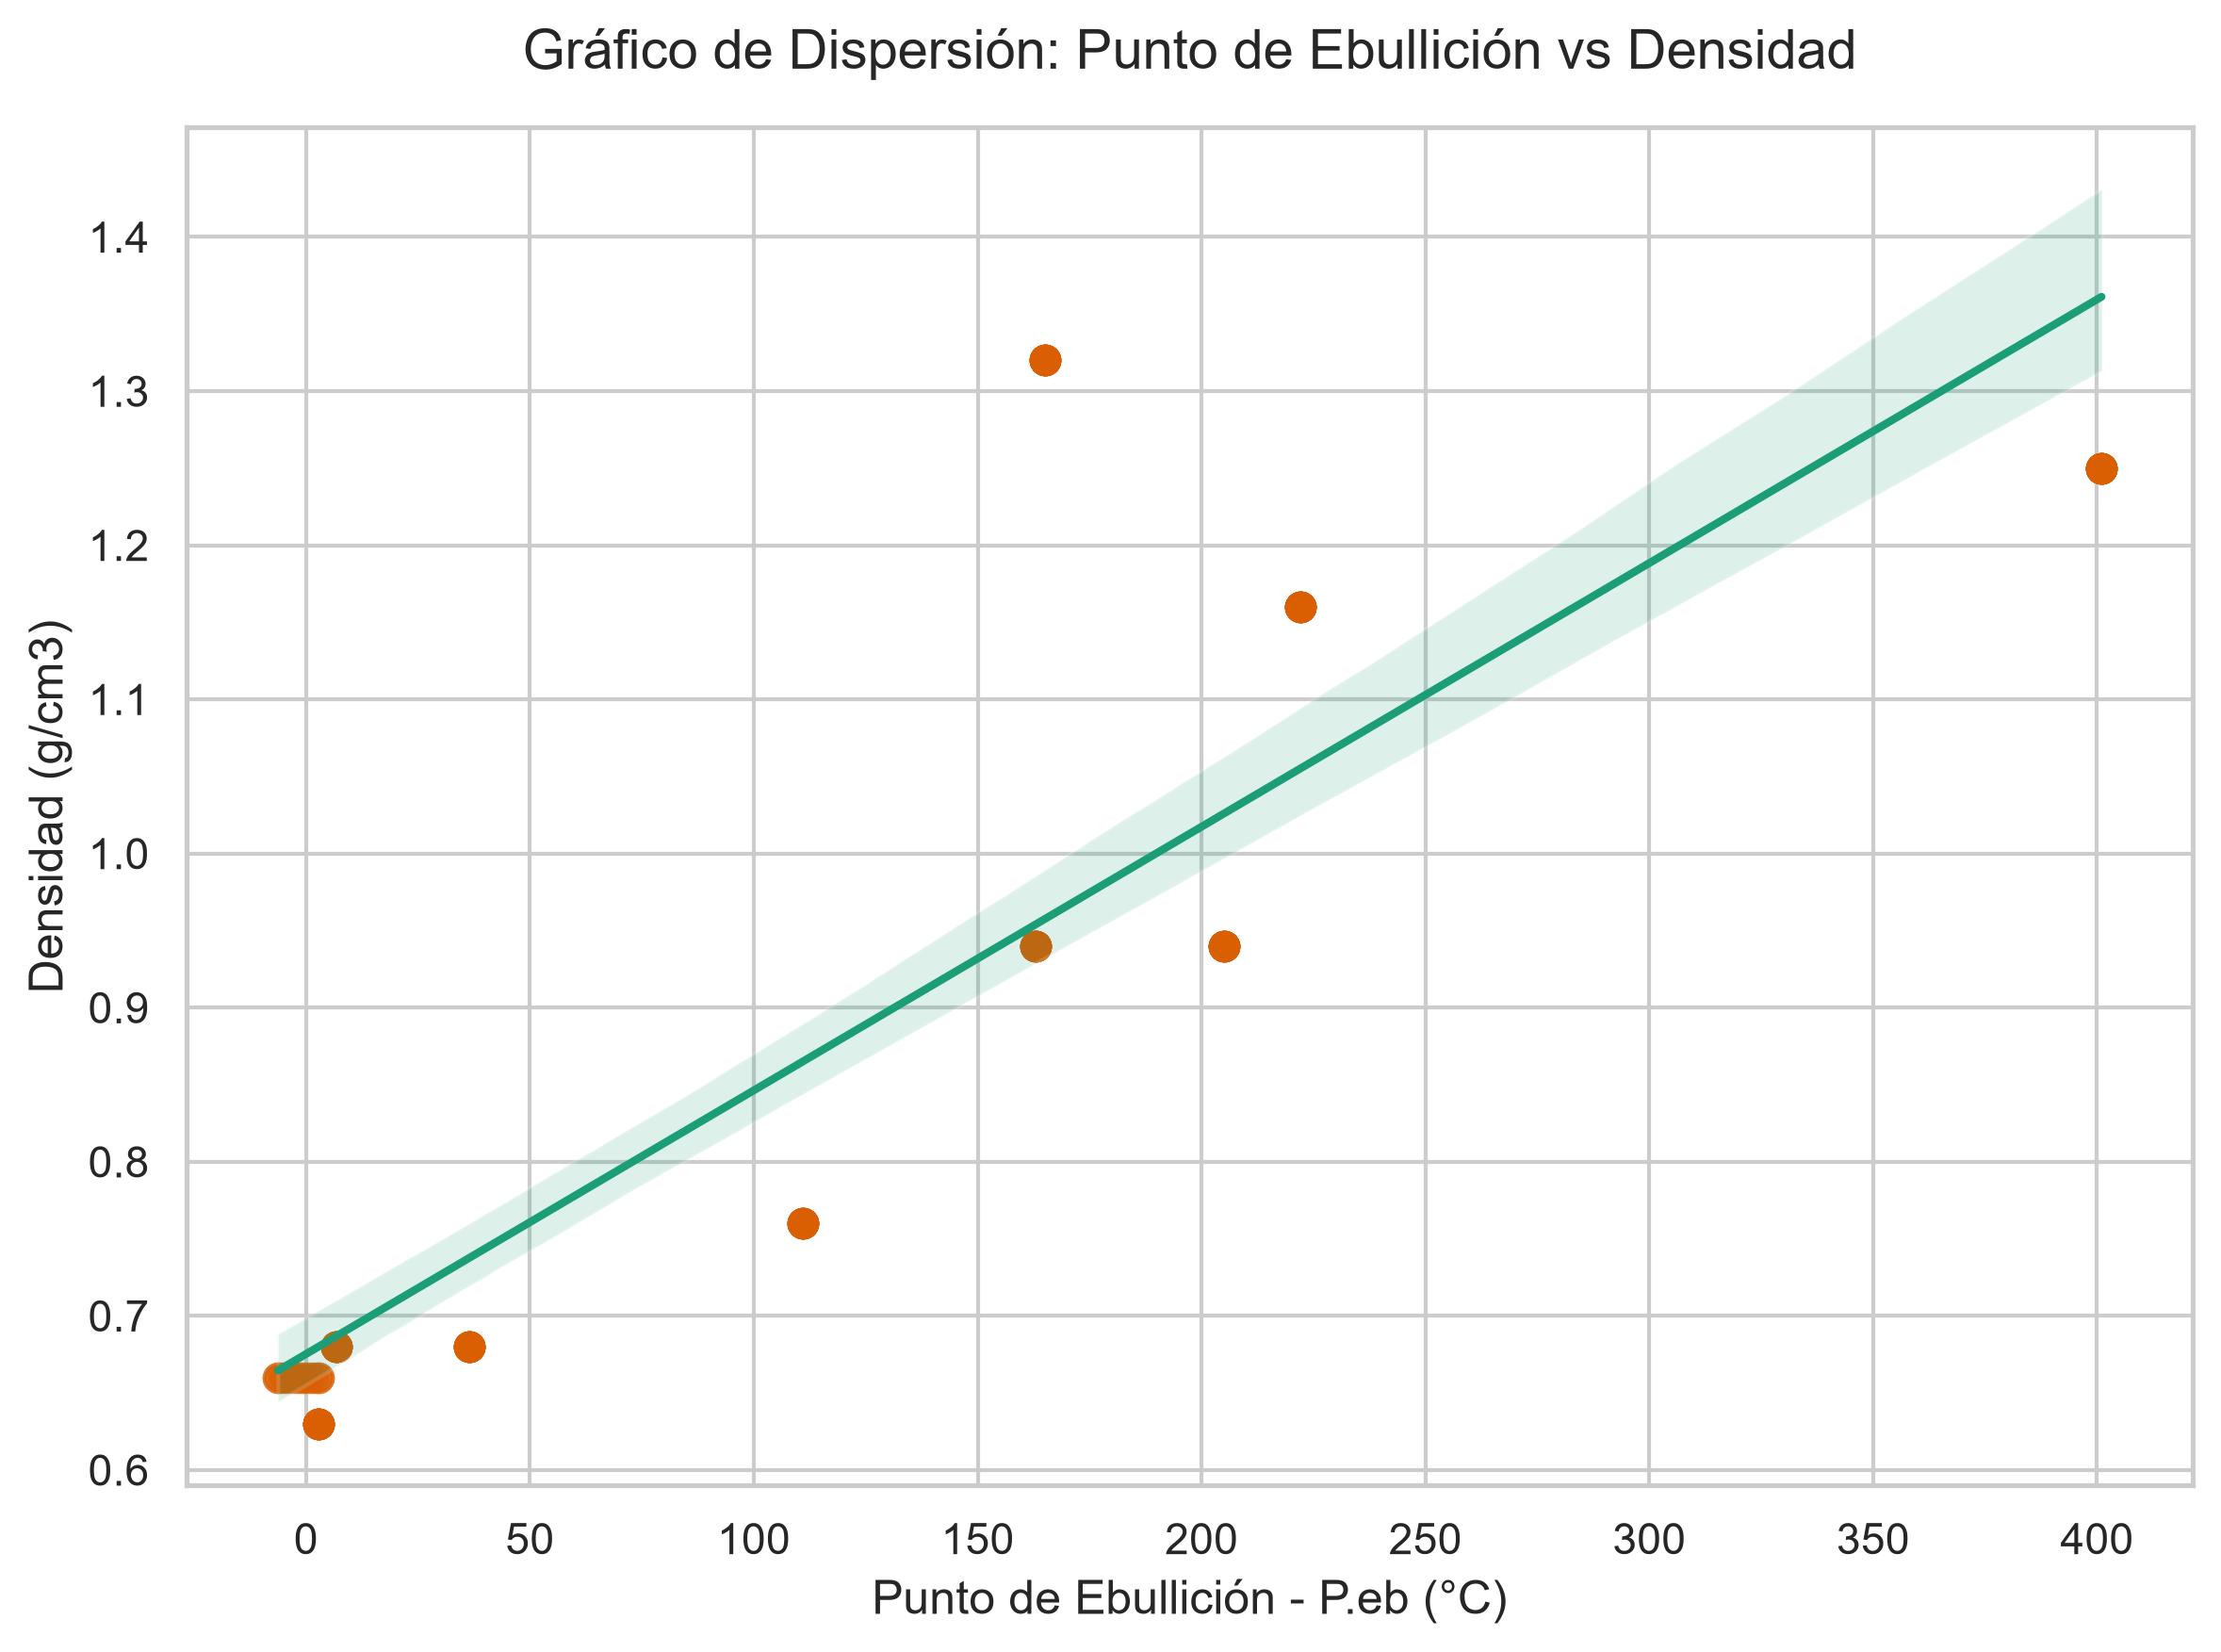
\includegraphics[width=\columnwidth]{04_reg_peb_vs_densidad.png}
	\caption{Punto de ebullición frente a densidad.}
	\label{fig:peb-dens}
\end{figure}

\begin{figure}[htbp]
	\centering
	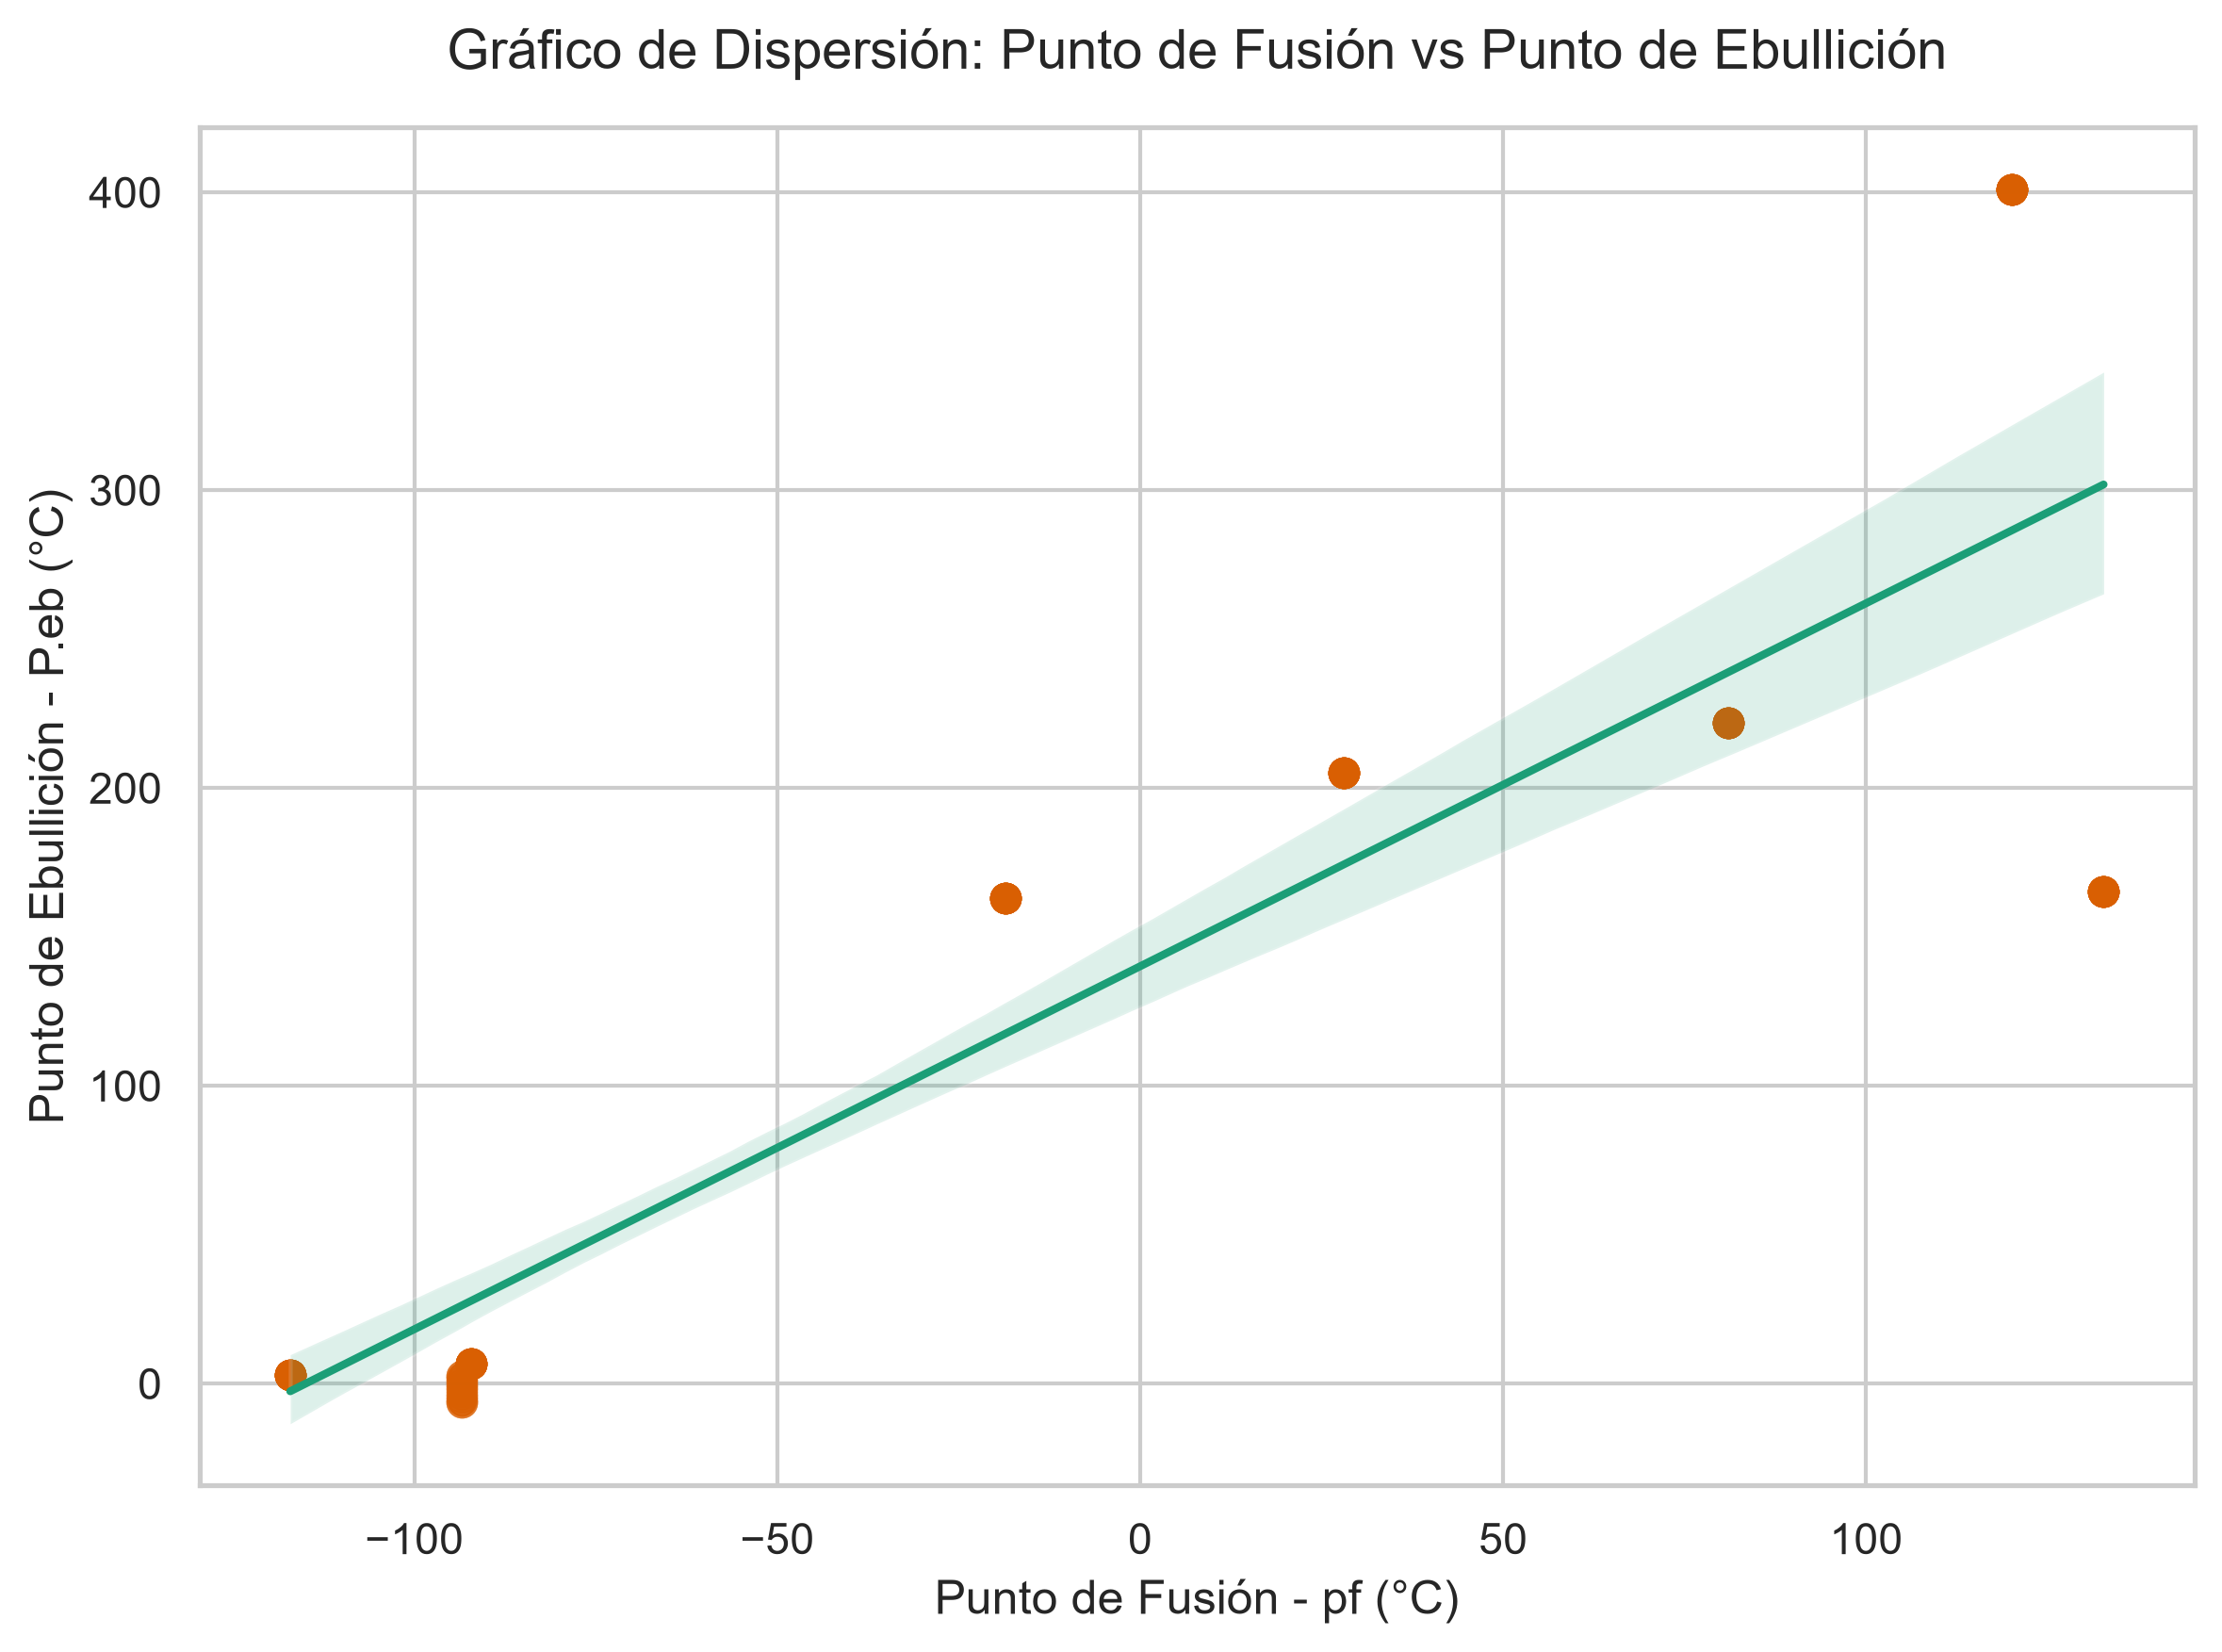
\includegraphics[width=\columnwidth]{05_reg_pf_vs_peb.png}
	\caption{Punto de fusión frente a punto de ebullición.}
	\label{fig:pf-peb}
\end{figure}

\begin{figure}[htbp]
	\centering
	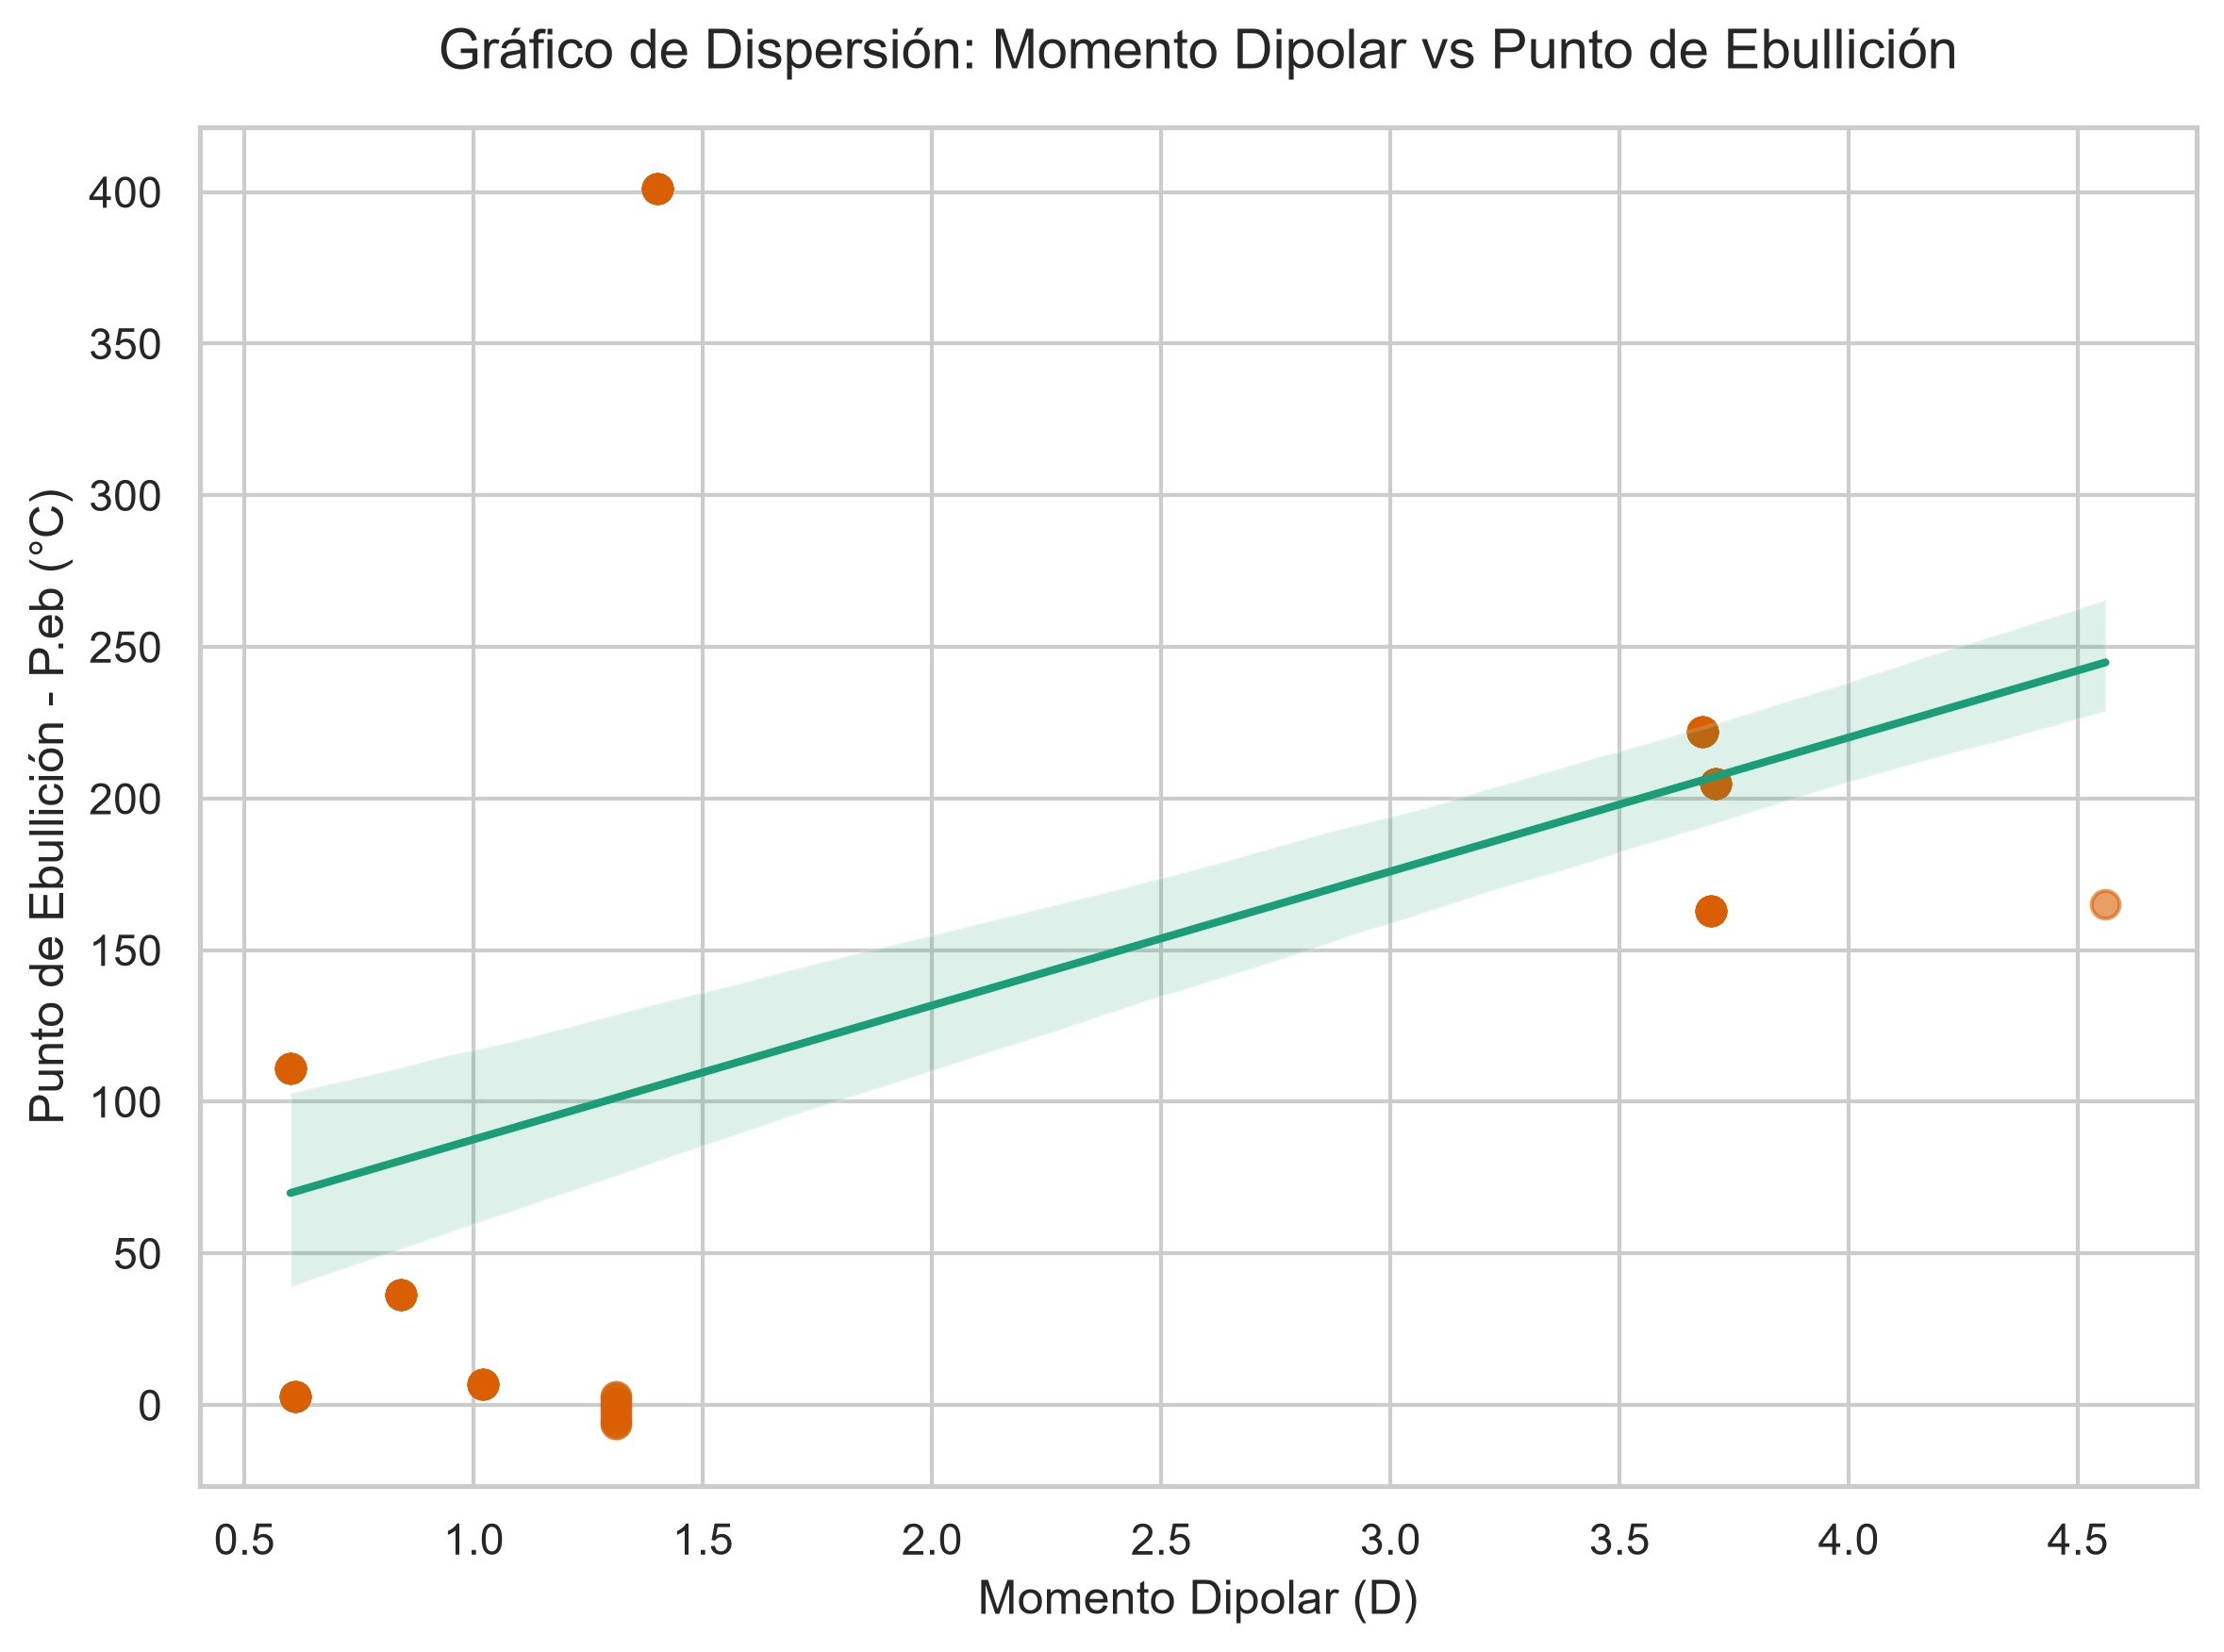
\includegraphics[width=\columnwidth]{06_reg_dipolo_vs_peb.png}
	\caption{Momento dipolar frente a punto de ebullición.}
	\label{fig:dip-peb}
\end{figure}

\subsection{Exploración interactiva con Plotly}
% TODO (Valentina): interpretar; idea central: a igual PM, los compuestos con
% enlace N--H (donadores de puente de H) hierven mucho más alto.
Las Figuras~\ref{fig:burbujas}--\ref{fig:dens-sol} se generaron con Plotly,
una fila por compuesto; sus versiones HTML permiten inspeccionar cada molécula
con el cursor. En la Figura~\ref{fig:burbujas}, trimetilamina
(\SI{2.8}{\degreeCelsius}) y N-metiletanamina (\SI{36.5}{\degreeCelsius}) tienen
el mismo peso molecular (\SI{59.11}{\gram\per\mole}): la diferencia se debe a que
sólo la segunda posee enlace N--H y forma puentes de hidrógeno.
\textit{[Interpretación pendiente.]}

\begin{figure}[htbp]
	\centering
	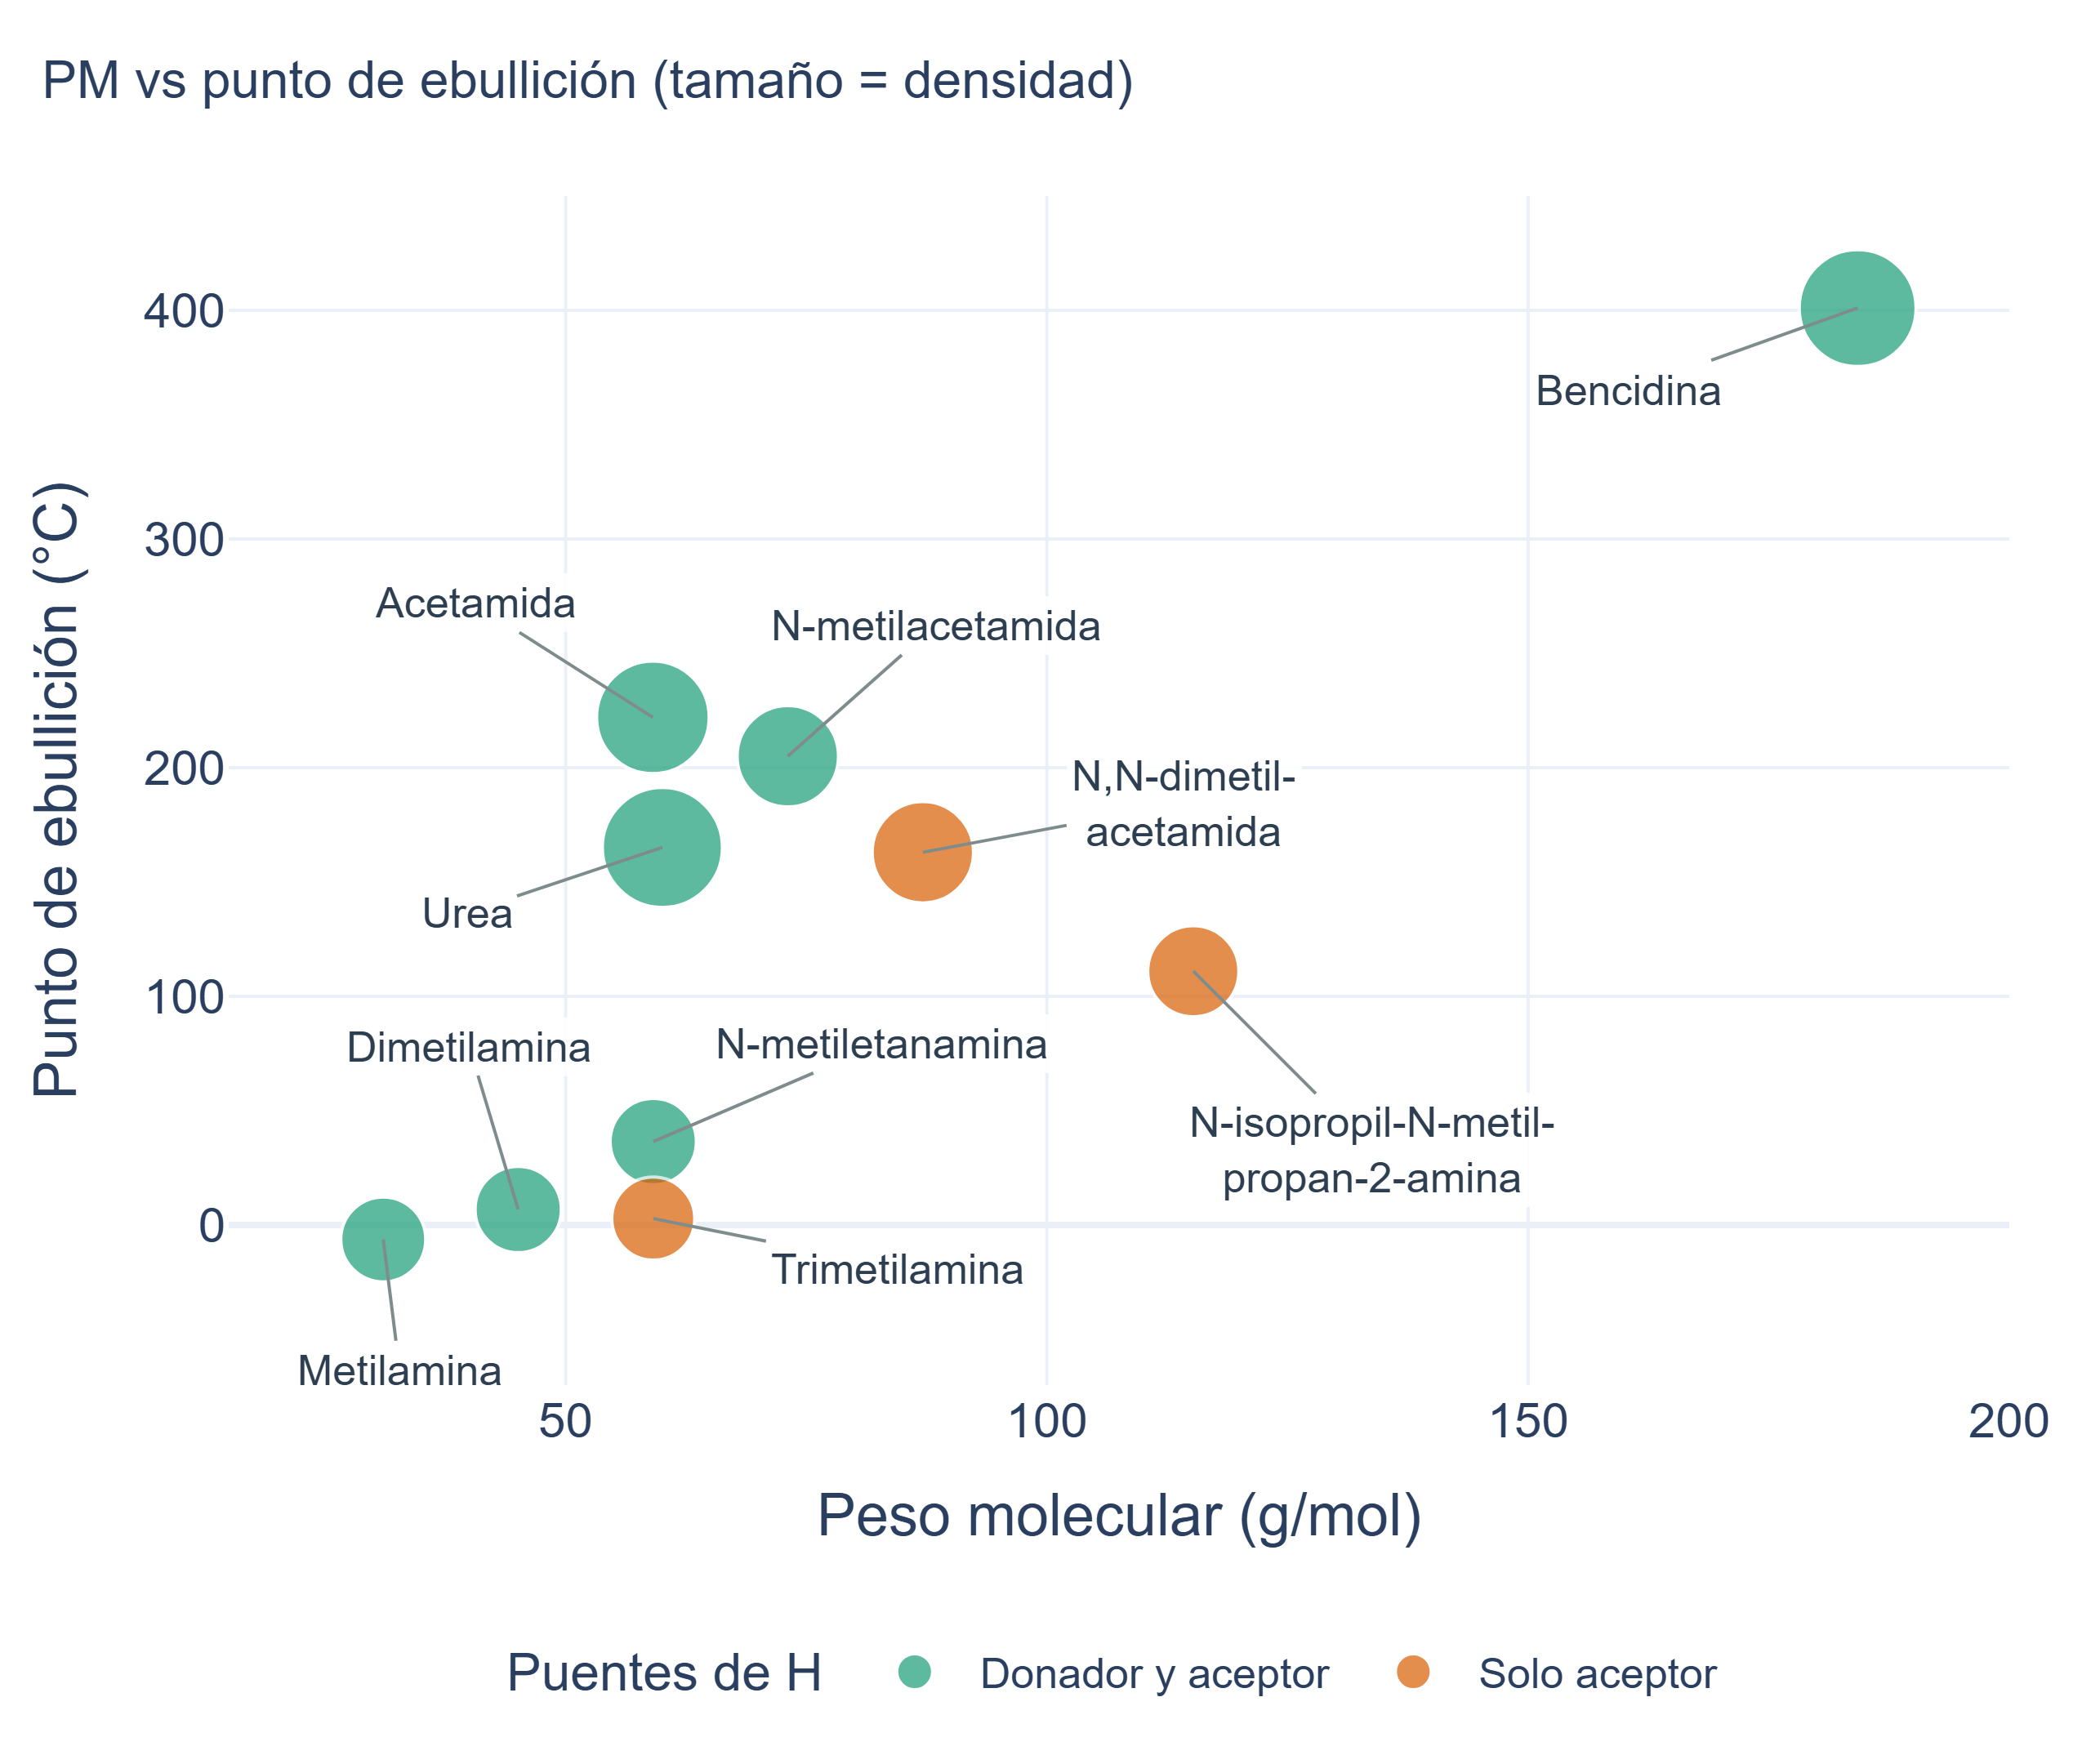
\includegraphics[width=\columnwidth]{11_plotly_burbujas_pm_peb.png}
	\caption{Peso molecular frente a punto de ebullición; el tamaño representa la densidad y el color la capacidad de formar puentes de hidrógeno.}
	\label{fig:burbujas}
\end{figure}

\begin{figure}[htbp]
	\centering
	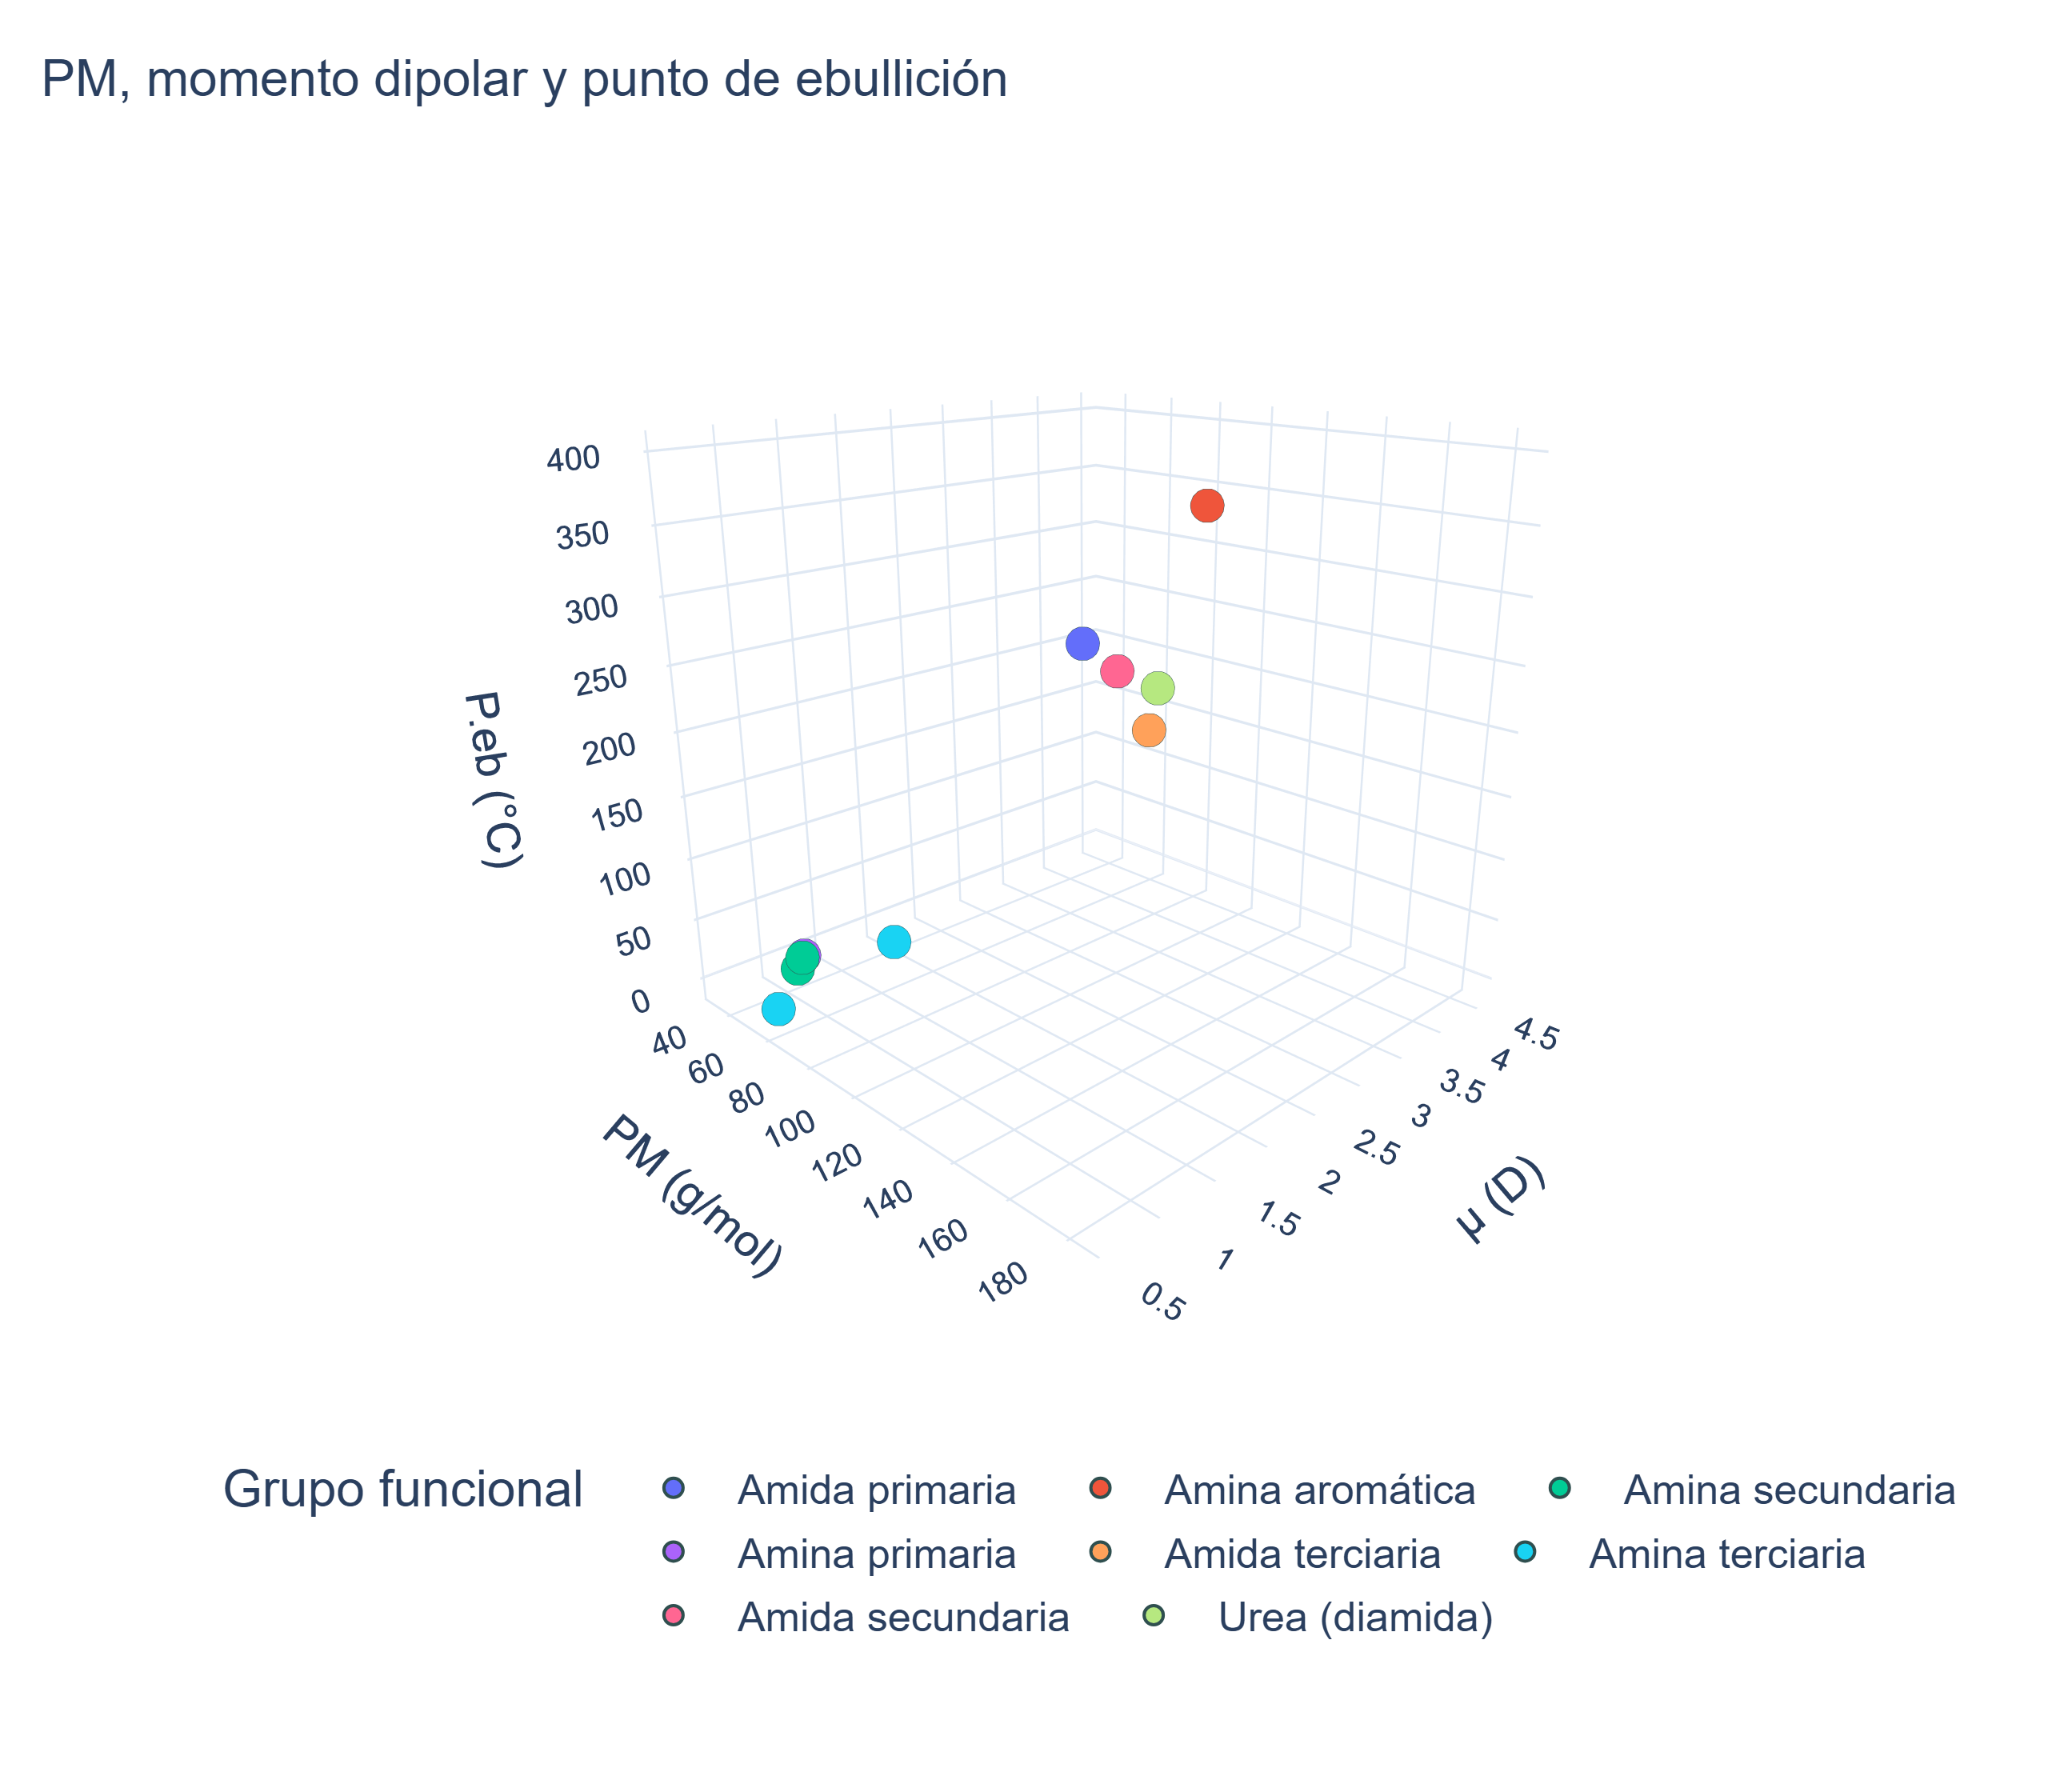
\includegraphics[width=\columnwidth]{12_plotly_3d_pm_dipolo_peb.png}
	\caption{Espacio tridimensional de peso molecular, momento dipolar y punto de ebullición por grupo funcional.}
	\label{fig:3d}
\end{figure}

\begin{figure}[htbp]
	\centering
	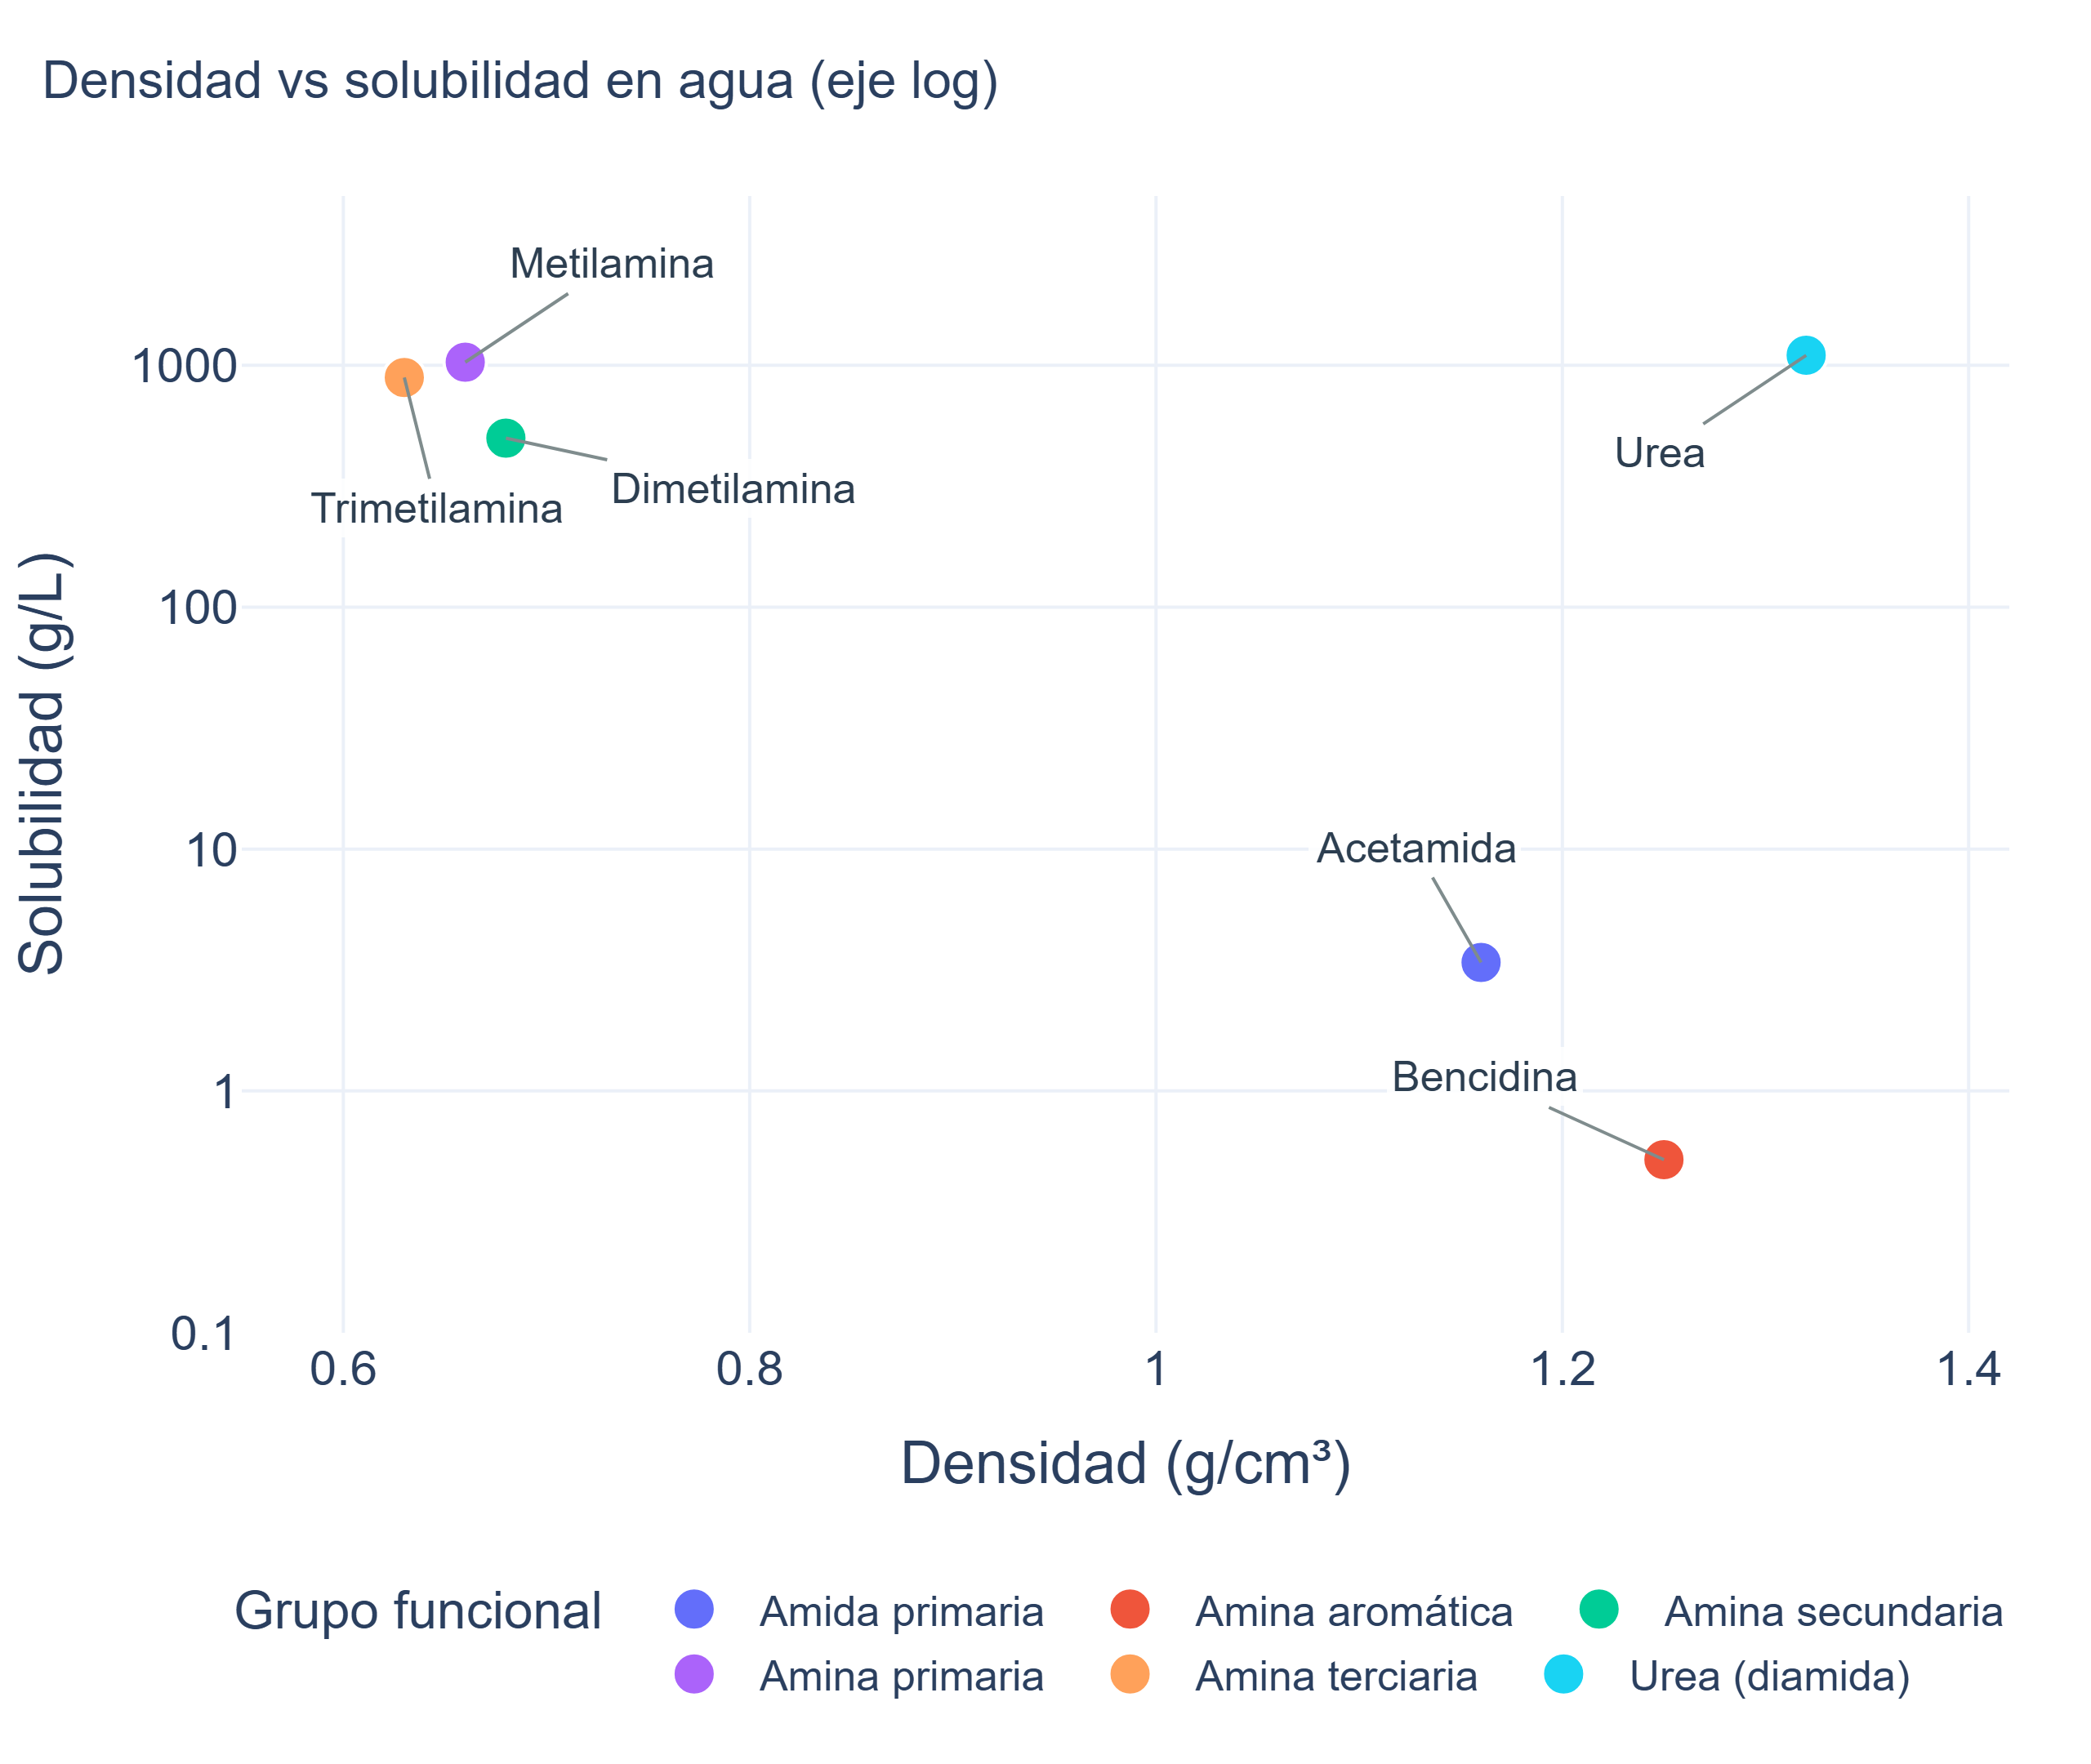
\includegraphics[width=\columnwidth]{13_plotly_densidad_solubilidad.png}
	\caption{Densidad frente a solubilidad en agua (eje logarítmico).}
	\label{fig:dens-sol}
\end{figure}

\subsection{Distribución por tipo de reacción y medio}
% TODO (Valentina): explicar qué representa TR y comparar medianas/dispersiones.
La Figura~\ref{fig:frecuencias} compara la frecuencia de cada mecanismo de
reacción y de cada medio; la sustitución nucleofílica (SN) domina, coherente con
el carácter nucleófilo del par libre del nitrógeno. Las
Figuras~\ref{fig:violin}--\ref{fig:dona} describen la distribución de
probabilidad de TR según el tipo de reacción y el medio.
\textit{[Interpretación pendiente.]}

\begin{figure}[htbp]
	\centering
	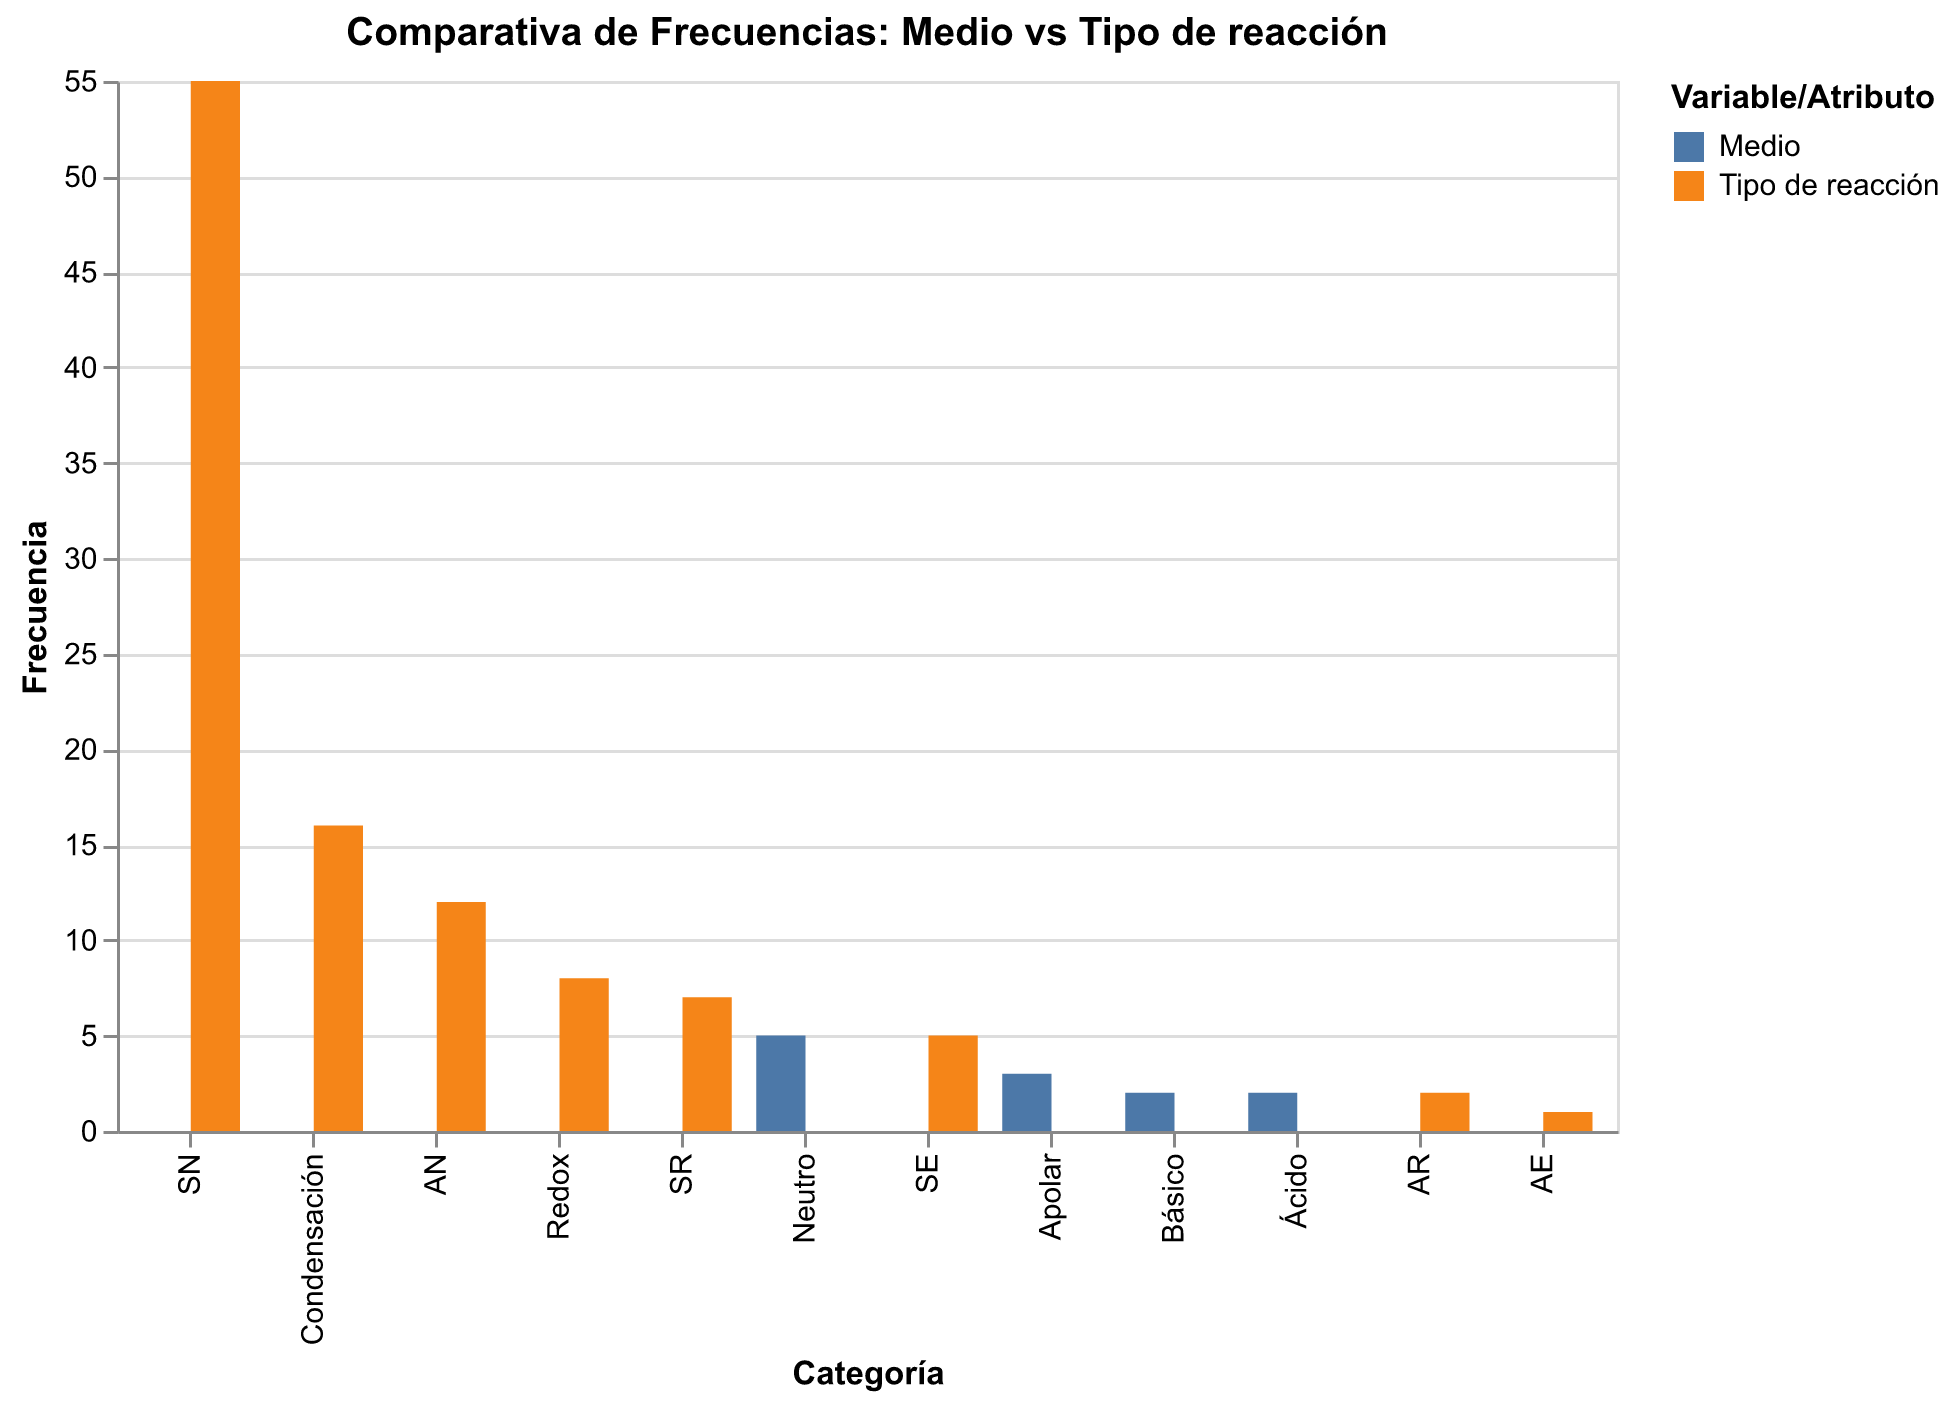
\includegraphics[width=\columnwidth]{09_frecuencias_medio_tipo.png}
	\caption{Frecuencia de los tipos de reacción y de los medios reportados.}
	\label{fig:frecuencias}
\end{figure}

\begin{figure}[htbp]
	\centering
	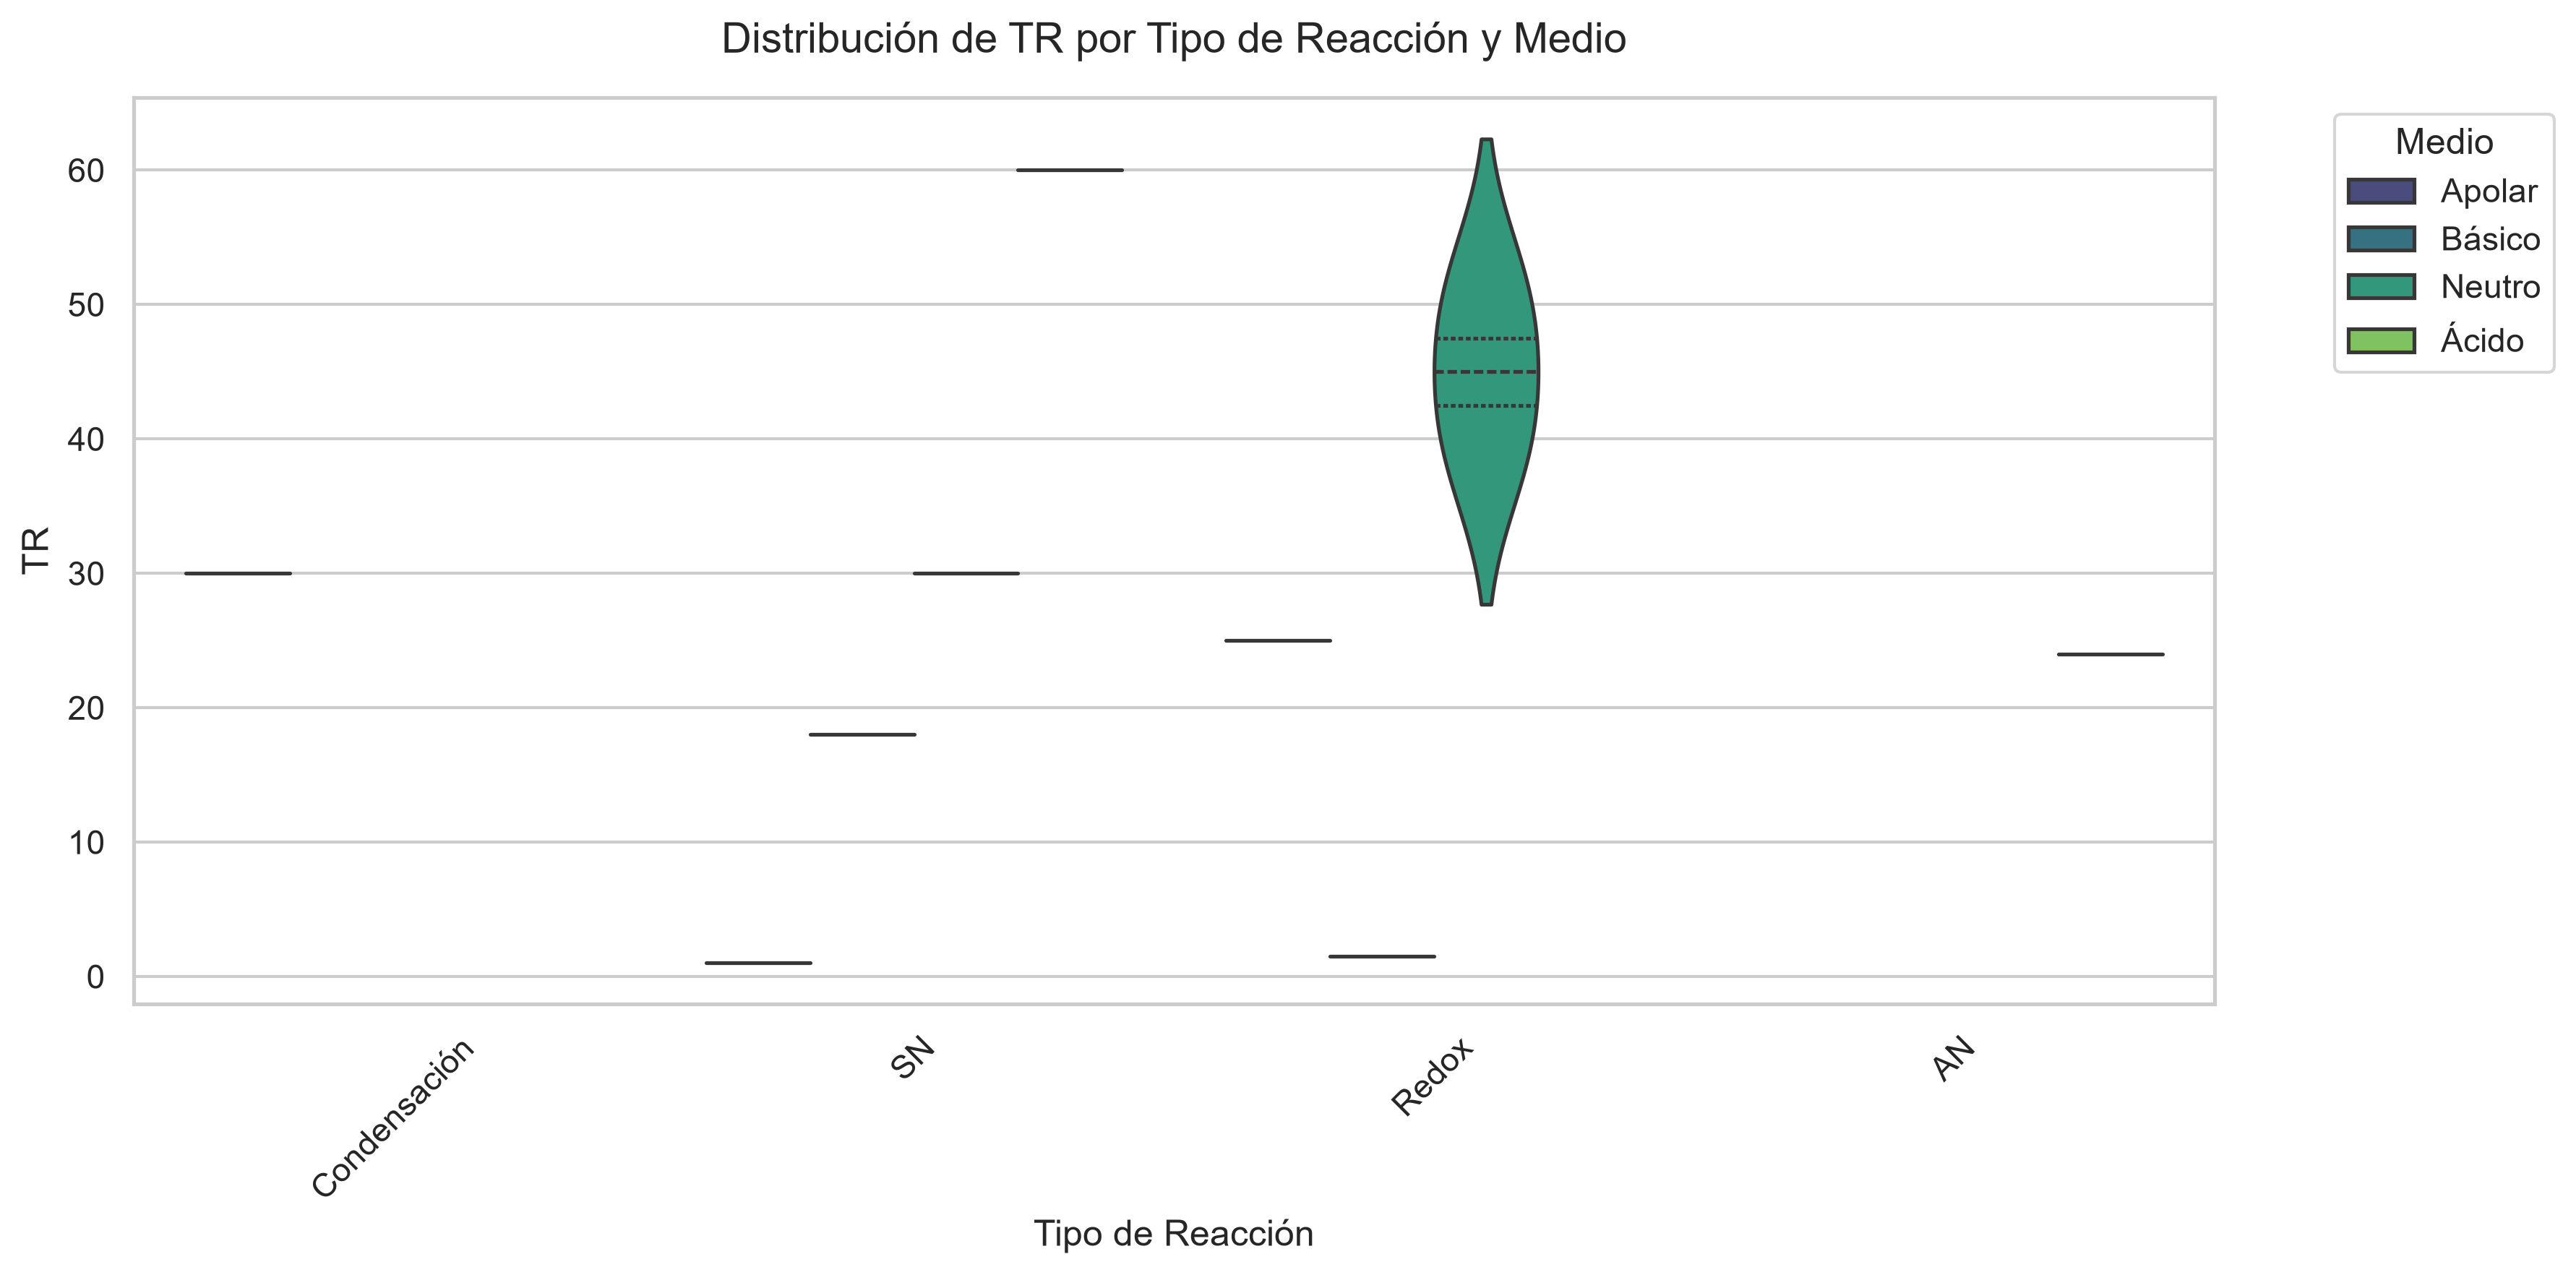
\includegraphics[width=\columnwidth]{07_violin_TR_tipo_medio.png}
	\caption{Distribución (violín) de TR por tipo de reacción y medio.}
	\label{fig:violin}
\end{figure}

\begin{figure}[htbp]
	\centering
	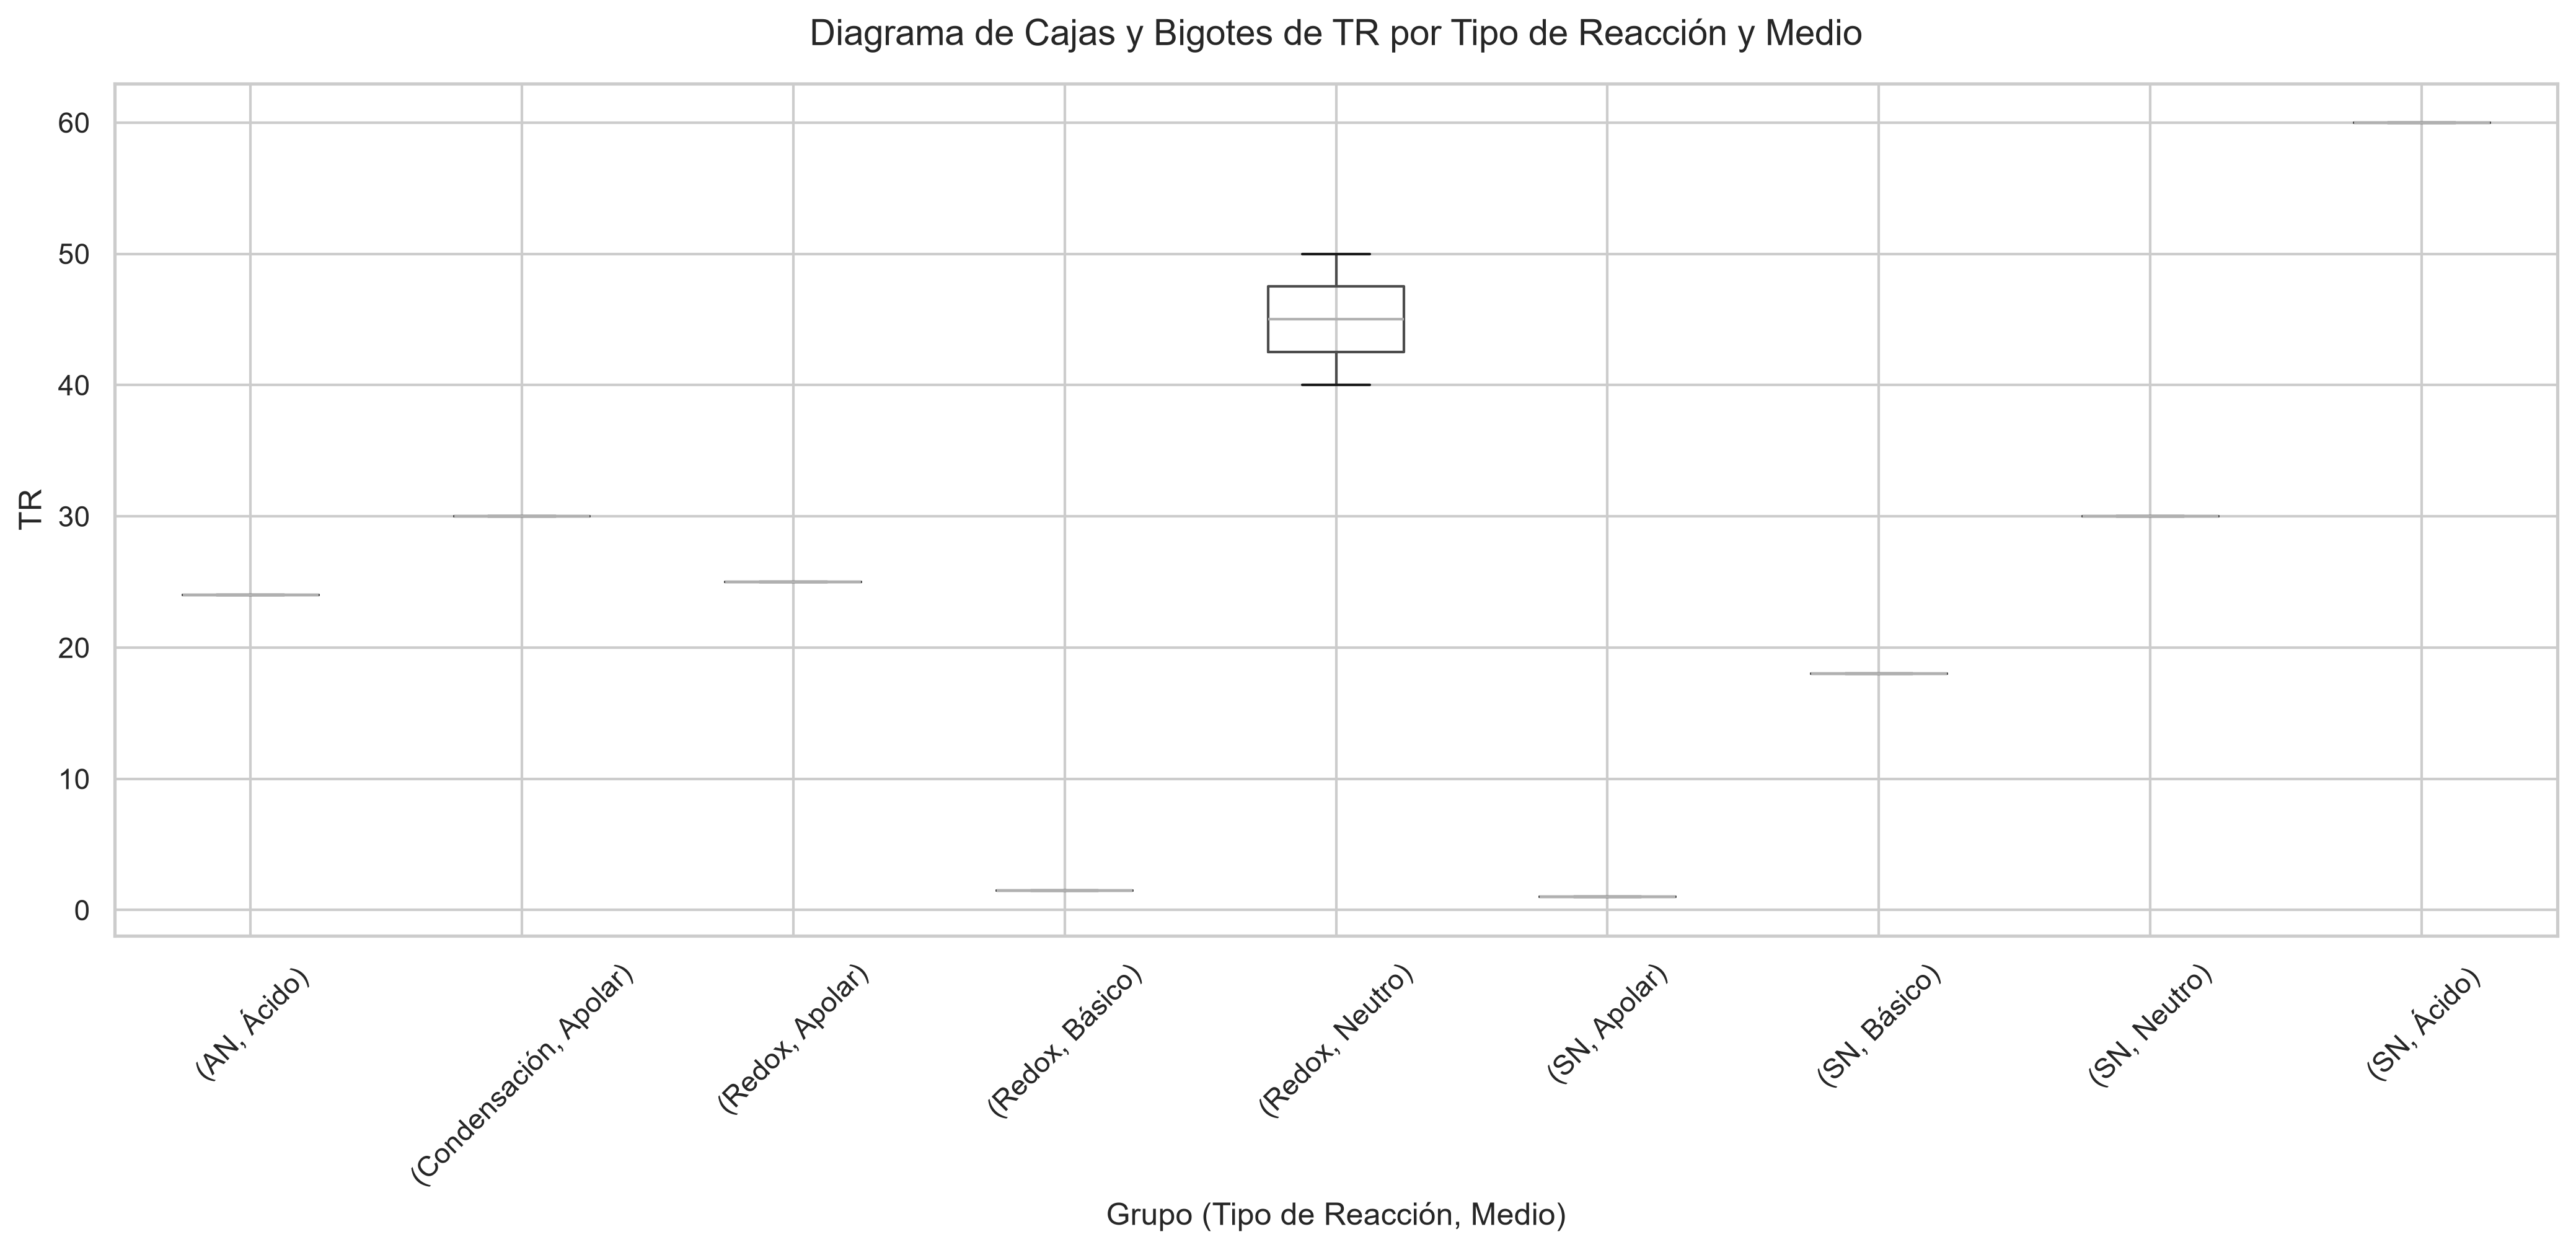
\includegraphics[width=\columnwidth]{08_boxplot_TR_tipo_medio.png}
	\caption{Diagrama de cajas y bigotes de TR por tipo de reacción y medio.}
	\label{fig:boxplot}
\end{figure}

\begin{figure}[htbp]
	\centering
	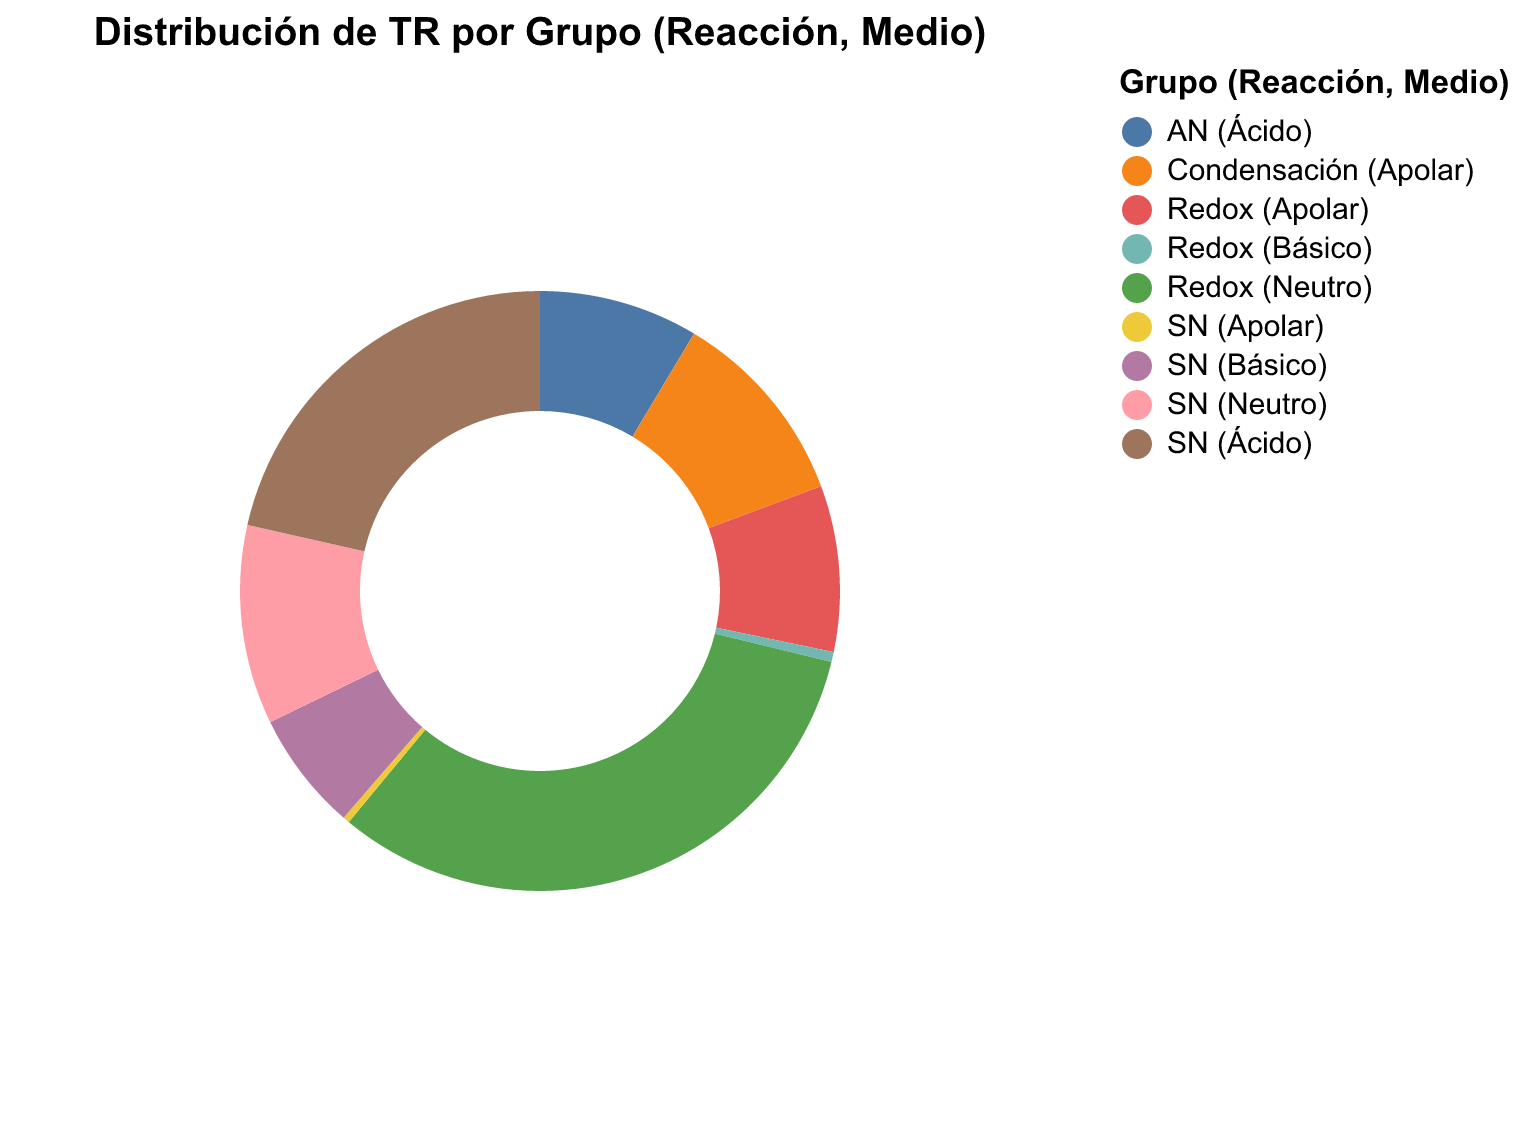
\includegraphics[width=0.9\columnwidth]{10_dona_TR_grupo.png}
	\caption{Participación de TR por grupo (tipo de reacción, medio).}
	\label{fig:dona}
\end{figure}

\section{Conclusiones y Perspectiva}
\fontsize{12}{14}\selectfont
% TODO (Valentina): 3--5 conclusiones que respondan al objetivo de la introducción,
% cada una sustentada en una figura o en la Tabla~\ref{tab:propiedades}.
\textit{[Redacción pendiente.]}


% ---------------------------------------------------------------------
%  DECLARACIÓN Y BIBLIOGRAFÍA (compartidas)
% ---------------------------------------------------------------------
\section{Declaración}
\fontsize{11}{13}\selectfont

\textbf{Conflicto de intereses:} Los autores declaran no tener conflictos de intereses.

\textbf{Contribución de los autores:}
Sara [Apellido]: introducción, marco teórico y tabla de datos.
Valentina [Apellido]: metodología, análisis gráfico y conclusiones.
[Tercer integrante]: recolección en CAS-SciFinder, dashboard de Power BI y repositorio GitHub.

\printbibliography[title={Referencias}]

\end{document}
